\documentclass[11pt]{article}
\usepackage{debulletin,times,epsfig,subfigure,wrapfig,color,boxedminipage,graphicx,url}

\usepackage{tabu}
\usepackage{multirow}
\usepackage{ulem}
\usepackage[utf8]{inputenc}

\usepackage{amsmath, amssymb, amsfonts}

\usepackage{hyperref}
\usepackage{enumitem}
\usepackage{xspace}
%\usepackage{xcolor}
\usepackage{tikz}
\usepackage[T1]{fontenc}
\usepackage{beramono}
\usepackage{listings}
\usepackage{xcolor}
\usepackage{wrapfig}
\usepackage{graphics}
\usepackage{pifont}
\usepackage[numbers]{natbib}
\usepackage{microtype}
\usepackage{graphicx}
\usepackage{subfigure}
\usepackage{booktabs} % for professional tables
\usepackage{epsfig}
\usepackage{pgfplotstable}
\usepackage{pgfplots}
\usepgfplotslibrary{groupplots}
\usepackage{bbm}
\usepackage{booktabs}
\usepackage{verbatim}
\usepackage[T1]{fontenc}
\usepackage{caption}
\usepackage{siunitx}
\usepackage{xspace}
\usepackage[autostyle, english=american]{csquotes}
\usepackage{breakurl}
%\usepackage{algorithm}
%\usepackage{algorithmic}
%\usepackage[algo2e]{algorithm2e}

\usepackage{makecell}
\usepackage{changepage}
\usepackage{diagbox}




\usepackage{times,graphicx}
\usepackage{multirow}
\usepackage{booktabs}
\usepackage{caption}
\usepackage{enumitem}
\usepackage[T1]{fontenc}    % use 8-bit T1 fonts
\usepackage{url}            % simple URL typesetting
\usepackage{nicefrac}       % compact symbols for 1/2, etc.
\usepackage{microtype}      % microtypography
\usepackage{xcolor}         % colors
\usepackage{bm}
\usepackage{amsmath,amssymb}
\usepackage{algorithm}
\usepackage[noend]{algpseudocode}
\usepackage{soul}
\usepackage{xspace}
\usepackage{makecell}
\usepackage{ulem}
\DeclareMathOperator{\round}{round}
\DeclareMathOperator{\clamp}{clamp}

\usepackage{times,graphicx}
\usepackage[utf8]{inputenc} % allow utf-8 input
\usepackage[T1]{fontenc}    % use 8-bit T1 fonts
\usepackage{url}            % simple URL typesetting
\usepackage{booktabs}       % professional-quality tables
\usepackage{amsfonts}       % blackboard math symbols
\usepackage{nicefrac}       % compact symbols for 1/2, etc.
\usepackage{microtype}      % microtypography
\usepackage{xcolor}         % colors
\usepackage{graphicx}
\usepackage{caption}
\usepackage{enumitem}
\usepackage{caption}
%\usepackage{subcaption}
%\usepackage[margins=normal,leading=normal]{savetrees} % conservatively saving space

\usepackage{grffile}

\usepackage{tablefootnote}

\usepackage{amsmath, amsfonts, amssymb}
\usepackage{cleveref}
\usepackage{nicefrac}       % compact symbols for 1/2, etc.
\usepackage{microtype}      % microtypography
\usepackage{xcolor}         % colors
\usepackage{bbm}
% %\usepackage{algpseudocode, algorithmicx}
% %\renewcommand{\algorithmicrequire}{\textbf{Input:}}
\usepackage{placeins}
\usepackage{tabularx}
\usepackage{makecell}
\usepackage{threeparttable}



\begin{document}


% please enter real date, vol no, issue no
\bulletindate{March 2021}
\bulletinvolume{44}
\bulletinnumber{1}
\bulletinyear{2021}

% these are files that I have- but your part of the issue can be done without
% them
\IEEElogo{cs.pdf}
\insidefrontcover{incvA19.pdf}
%\insidebackcover[ICDE Conference]{./calls/icde-new-a.ps}

\begin{bulletin}

% the above samples assume the issue is generated from a directory structure of the following sort
% major directory name is month and year of issue
% there are sub-directorys for
% letters: directory name is "letters"
% technical articles: a directory per paper, named for an "author"
% news articles: directory name is "news"
% calls: directory name is "calls

%
%  Editor letters section.  Use the lettersection environment.
%  Each letter is contained in a letter environment, where the two required
%  options to \begin{letter} are the author and the address of the author.
%

\begin{lettersection}

% there will be other letters- and a blank page will appear in your document
% but the special issue part will be fine

\begin{letter}{Letter from the Editor-in-Chief}
{Haixun Wang}{Instacart}
\documentclass[11pt]{article} 

\usepackage{deauthor,times,graphicx}
%\usepackage{url}
\usepackage{hyperref}

\begin{document}
Around the time we published our last issue in March, the nation went
into a lockdown. Life in the last 3 months has been unprecedented in
many ways. As governments around the world scrambled to fight
coronavirus, people in the scientific community, especially those on
the frontline -- doctors, healthcare professionals, medical staff and
researchers -- made heroic efforts and sacrifices to curb the pandemic
and save lives. The data management and data science communities also
sprang to action immediately. Globally, it is the first time that data
driven approaches are being used at such a large scale toward solving
a common problem. Under this backdrop, in this special issue of the
Data Engineering Bulletin edited by Joseph Gonzalez, we feature 8
papers on the topic of {\it digital contact tracing}, a technique that
may prove crucial in the fight against Covid-19.

This issue also features two opinion pieces. Divyakant Agrawal and Amr
El Abbadi's wake-up call on managing data in an untrusted environment
takes us to the fascinating world of cryptocurrencies and
blockchains. It shows what the database community, which was
responsible for creating and perfecting transaction management and
distributed systems, can learn from the blockchain approach when it
comes to handling untrusted behaviours from the underlying
infrastructure. The second opinion piece, written by Jeffrey
D. Ullman, addresses a question on the mind of every data management
person: What is our role in the machine learning and AI revolution?
Have we missed the boat again and become irrelevant? Ullman's
perspective, illustrated by his remake of the well known Conway Venn
Diagram that illustrates the relationship between computer science,
mathematics \& statistics, and domain knowledge is incisive,
thought-provoking, and entertaining at the same time.
\end{document}


\end{letter}
%
\newpage
%
%% your introductory letter goes here
%
%\begin{letter}{Letter from the Special Issue Editor}
\begin{letter}{Letter from the Special Issue Editor} %JF: made it editors, plural
{Yangqiu Song}{The Hong Kong University of Science and Technology}
\documentclass[11pt]{article}

\usepackage{deauthor,times,graphicx}
%\usepackage{url}

\begin{document}
Similarity search in high-dimensional data spaces was a relevant and challenging data management problem in the early 1970s, when the first solutions to this problem were proposed. 
Today, fifty years later, we can safely say that the exact same problem is more relevant and challenging than ever. 
This is true, not because the research community has been idle; on the contrary, the literature on this topic is very large and diverse, demonstrating both the interest in this problem, as well as the wide range of ideas that have been applied to it and led to impressive advances. 
This is true, rather because very large amounts of high-dimensional data are now omnipresent (ranging from traditional multidimensional data to time series and deep embeddings), and the performance requirements (in terms of both response-time and accuracy) of a variety of applications that need to process and analyze these data have become very stringent and demanding.

In these past fifty years, high-dimensional similarity search has been studied in its many flavors. Similarity search algorithms for exact and approximate, one-off and progressive query answering. 
Approximate algorithms with and without (deterministic or probabilistic) quality guarantees.
Solutions for on-disk and in-memory data, static and streaming data.
Approaches based on multidimensional space-partitioning and metric trees, random projections and locality-sensitive hashing (LSH), product quantization (PQ) and inverted files, k-nearest neighbor graphs and optimized linear scans.

Another interesting aspect of the work in high-dimensional similarity search is that research on this problem has been conducted by different (sub-)communities in a somewhat independent fashion, that is, with not much interaction among them.
A notable example is the work on data-series (and time-series) similarity search, which was recently shown to achieve the state-of-the-art performance for several variations of the problem, on both time-series and general high-dimensional vector data.
It is only very recently that a conscious effort is being made in order to gather the state-of-the-art methods from these different communities, and thus, enable the comparison of the various approaches, the extraction of useful insights, and the development of improved solutions.
This special issue contributes to this effort by including a selection of papers that represent the research activity in several of these communities, highlighting similarities and differences, and revealing open research directions.

In the first paper, Wang et al. summarize and discuss state-of-the-art solutions for approximate similarity search based on k-nearest neighbor graphs and data-series tree indexes, and point to promising research directions.
In the second paper, Zhang et al. list the similarity search requirements of modern applications, and present novel algorithms based on k-nearest neighbor graphs that exploit multi-core architectures and NVMe memory.
In the third paper, Tian et al. summarize and discuss state-of-the-art solutions, as well as future research directions, for approximate similarity search based on locality-sensitive hashing, product quantization and k-nearest neighbor graphs.
In the fourth paper, Dong et al. propose the use of neural networks in order to learn effective space partitions, and develop a novel solution based on locality-sensitive hashing for approximate similarity search.
In the fifth paper, Paparrizos et al. compare many distance measures proposed for time-series similarity search, comment on the lower bounds that speedup some of these measures, and discuss the open research problems that their findings point to. 
Finally, in the sixth paper, Aum\"{u}ller and Ceccarello study the very important problem of creating appropriate benchmarks for approximate similarity search; they review recent benchmarks, and offer guidelines for future efforts in this area.

Overall, we believe that the above papers represent an interesting sample of the ongoing work on high-dimensional similarity search. 
We hope that this special issue will further help and inspire the research community in its quest to solve this challenging problem.

We would like to thank all the authors for their valuable contributions, as well as Haixun Wang for giving us the opportunity to put together this special issue, and Nurendra Choudhary for his help in its publication.

Themis Palpanas

Universit{\'e} Paris Cit{\'e}
\end{document}


\end{letter}

\end{lettersection}



\begin{articlesection}{Learning and Reasoning on Knowledge Graphs and Applications}
%
%  Contributed articles section.  Use the articlesection environment.
%  Each article is contained in an article environment, where the two required
%  options to \begin{article} are the title and author of the article
%

%\makeatletter
%\renewcommand{\AB@affillist}{}
%\renewcommand{\AB@authlist}{}
%\setcounter{authors}{0}
%\makeatother

% \begin{article}
% {Transforming the Culture: Internet Research at the Crossroads}
% {Safiya Umoja Noble and Sarah T. Roberts}
% \graphicspath{{submissions/NobleRoberts_final/}}
% %\documentclass[11pt,dvipdfm]{article}
\documentclass[11pt]{article}
\usepackage{deauthor,times,graphicx,hyperref} 

\usepackage{amsmath, amssymb, amsfonts}  

%\usepackage{algorithmic}
%\usepackage{graphicx}
%\usepackage{textcomp}
%\usepackage{xcolor}
\def\BibTeX{{\rm B\kern-.05em{\sc i\kern-.025em b}\kern-.08em
    T\kern-.1667em\lower.7ex\hbox{E}\kern-.125emX}}

%\usepackage{graphicx}
%\usepackage{subfigure}
%\usepackage{hyperref}
%\usepackage{enumitem}
%\usepackage{multirow}
%\usepackage{dsfont}
%\usepackage{algorithm2e}
%\usepackage[table,xcdraw]{xcolor}
%\usepackage{booktabs}

%\usepackage{tikz}
%\usetikzlibrary{bayesnet}

\usepackage{breakcites} %Fixes citations exceeding the margin!!

% \newtheorem{example}{Example} 
% \newtheorem{theorem}{Theorem}
% \newtheorem{lemma}[theorem]{Lemma} 
% \newtheorem{proposition}[theorem]{Proposition} 
 %\newtheorem{remark}[theorem]{Remark}
% \newtheorem{corollary}[theorem]{Corollary}
% \newtheorem{definition}[theorem]{Definition}
% \newtheorem{conjecture}[theorem]{Conjecture}
% \newtheorem{axiom}[theorem]{Axiom}
%%%
%\newtheorem{dfn}[theorem]{Definition}

%\usepackage{todonotes}
%\newcommand{\jf}[1]{{\bf \color{orange}{jf: #1}}}
%\newcommand{\shimei}[1]{{\bf \color{blue}{shimei: #1}}}
\setcounter{topnumber}{2}
\setcounter{bottomnumber}{2}
\setcounter{totalnumber}{4}
\renewcommand{\topfraction}{0.85}
\renewcommand{\bottomfraction}{0.85}
\renewcommand{\textfraction}{0.15}
\renewcommand{\floatpagefraction}{0.7}

% Definitions of handy macros can go here

\newcommand{\dataset}{{\cal D}}
\newcommand{\fracpartial}[2]{\frac{\partial #1}{\partial  #2}}

\begin{document}
\title{Transforming the Culture: Internet Research at the Crossroads}
\author{Safiya Umoja Noble \\
University of California, Los Angeles \\
snoble@g.ucla.edu
\and
Sarah T. Roberts\\ 
University of California, Los Angeles \\ 
sarah.roberts@ucla.edu}


\maketitle
\begin{abstract}
The topic of justice, fairness, bias, labor and their relation the products and practices of technology and internet companies has been a subject of our concern for nearly a decade. We see these challenges--from the organizing logics of the technology sector with respect to algorithmic discrimination, to labor practices in commercial content moderation, as key pathways into better understanding the creation and maintenance of problems made by the technology sector that cannot be solved with techno-solutionism. While our work has been closely aligned to research and advocacy broadly construed in the domain of ethics and AI, we seek to expand the conversations about sociotechnical systems beyond individual, moral and ethical concerns to those of structures, practices, policies which would allow for interdisciplinary frameworks from the fields of critical information studies, sociology, and the social sciences, and the humanities. To make legible the paradigm-shifting work we think could be taken up by scholars at colleges and universities, we will outline the contours and specifics of institutionalizing these approaches through a research center, the UCLA Center for Critical Internet Inquiry (C2i2) and its activities, By making visible the need for such a space, and our experiences and values, our hope is that it will make transparent the process and possibilities for centering justice and fairness in the world, rather than the prevailing technosolutionism we see emerging within conversations and initiatives focused on ethics and technology.
\end{abstract}

\section{Introduction}
In the summer of 2018, we received approval for the establishment of a new UCLA Center for Critical Internet Inquiry (C2i2). The proposed Center would be based within the Department of Information Studies, in the Graduate School of Education \& Information Studies, but would be campus-wide in scope, The effort was designed to address the societal impact of internet platforms, the social construction and effects of data they generate and disseminate, and their various drivers with a keen focus on issues of racial justice and gender equity. At the time of our founding, UCLA did not have any organized research unit that exclusively focused on this extraordinarily important and pervasive area of twenty-first century life, culture and economy. 

Our effort to develop and centralize a robust, visible institutional infrastructure at UCLA and beyond that provides researchers and instructors with a locus from which to inform internet development and policy, has not been without challenges. This work, by its very nature, challenges received notions of the internet and other digital technologies as primarily liberatory, beneficent or, at the least, value-neutral. Efforts to address the potentials and pitfalls of the internet for people and communities who are marginalized and underrepresented with respect to the digital is happening at a moment of austerity, when universities are increasingly reliant upon corporate and private donations to stay afloat in the wake of shrinking allocations from the legislators in Sacramento to its robust California Community Colleges, its world-class California State University system, and its flagship research campuses across the University of California.

\section{The State of Internet Research}
The public is increasingly eager to develop its own understanding and ability to actively participate in the steering of the digital technologies, social media platforms, and internet usage that now characterize much of everyday life, yet there are few mechanisms that afford such intervention. Those who should act in their stead, such as legislators and policy makers, legal professionals, educators, and others in gatekeeping capacities often lack a full picture of these technologies, their processes, and their social implications--even when they are sympathetic and energized to the public’s desire to wrest back control. For much of their existence, Silicon Valley’s social media firms have enjoyed close -- even cozy -- relationships with legislators in Washington. Even as the tide of general sentiment has turned over the past few years, the grilling that Senate subcommittees have intended to give the executives of those firms has often fallen flat simply due to a lack of precision or understanding on the part of the questioners. In both cases, the public has stood to lose.

Meanwhile, there has been an effort by these same firms, often along with university partners that have been heretofore largely uncritical of them, to get out ahead of any potential lawmaker curtailing their activities by appearing to self-regulate. The most common iteration of this attempt has come in the nascent development of a variety of “ethics” initiatives, boards and research teams popping up inside of and adjacent to the major corporations. Those initiatives, too, are not without significant flaws.  We are fundamentally concerned with the industry regulating itself in lieu of responding to public policy and providing accountability. While self-reflection is important, as are increasing efforts to broaden frameworks of responsibility, we largely see that self-regulation is insufficient as the industry leaders are the subjects of antitrust lawsuits, EEOC violations, and investigations into consumer harm.

We are indebted to a number of scholars who are influencing our thinking about the politics and power embedded in the digital, and whose work we are in dialog with on a continual basis ~\cite{benjamin2019race,chun2008control,daniels2009cyber,eubanks2018automating,hoffmann2019fairness,noble2018algorithms,pasquale2016black,roberts2019behind,vaidhyanathan2006afterword,vaidhyanathan2018antisocial}. There are of course, so many important social scientists and humanists whose work has been the opening for scholars in computing to take the systemic issues of fairness and equity. What we often find is that scholars in computer science and related engineering fields do not cite the work of the scholars who have framed the debate, thus making the need for epicenters of interdisciplinary critical scholarship even more crucial. Indeed, the ability to invoke issues of fairness has been made legible and plausible because humanists and social scientists have provided the evidence that has forced these issues into view. 


For instance, \cite{binns2018fairness}'s  review of ethics and fairness in the fields of machine learning and artificial intelligence is an important overview of how our colleagues in computing fields are increasingly limited by the origins of Western philosophy as they cultivate “ethical AI.” We will not repeat here the work done to trace the histories of liberalism and its limitations as applied to computing and digital technologies\footnote{See \cite{BuiNoble}.} , but we note that this previous careful study of the origins of liberal philosophy that bolsters the field of ethics deeply informs our own disposition toward the limits of this emerging field. In particular, we believe that the field of “ethical AI” must contend with how it affects and is affected by power structures that encode systems of sexism, racism, and class. Instead of depoliticizing these systems, we embrace a sociological orientation, in the tradition of scholars like \cite{daniels2009cyber}, who has adeptly framed and helped us better understand more powerful analytics like oppression and discrimination in lieu of words like bias and ethics, which obfuscate the power analyses and interventions so desperately needed. 


In our research, we use structural and systems-level analyses that can properly account for the impact of the socio-technical assemblages that make up digital  ecosystems and infrastructures. Through our studies of the digital, we uncover opportunities for accountability from harms that extend beyond individual moral and ethical choices to public policy, labor and employment practices, supply-chain business practices, environmental interactions, and a variety of approaches that can have tremendous impact at scale. Without these approaches, the work of ethical AI is greatly reduced to individual, technical, and organizational-level  failings against some imagined “fair” standard that, itself, is dislocated from fairness as a matter of civil, human, or sovereign rights tied to political, economic, and social struggles. Because of these analytical  framings, we are able to examine the material dimensions of internet-enabled digital infrastructures and practices that involve many factors that extend beyond algorithms and AI to include workers, legal and financial practices, and consolidations of power.   
\cite{BuiNoble} wrote about the way in which technology corporations, in an effort to minimize risk from the damages associated with their discriminatory and faulty products, are performing reputation management through claims to be more accountable, fair, transparent, and ethical. Several in-house ethical AI teams, corporate-sponsored research think tanks, and non-profits aligned with industry are producing myriad conferences, white papers, research publications and campaigns that seek to define the landscape of ethical AI. They note:
\begin{quote}
Moreover, data trusts and research partnerships between universities, policy think tanks, and technology corporations have been established and revamped as a go-to strategy for effecting a more democratic and inclusive mediated society, again calling for fairness, accountability, and transparency (FAT) as key ideals within the future of AI, yet often leaving and ignoring notions of intersectional power relations out of their ethical imaginaries and frameworks. As a point of departure, many are invested in linking conversations about ethics to the moral genesis and failures caused by structural racism, sexism, capitalism, and the fostering of inequality, with an eye toward understanding how the digital is implicated in social, political, and economic systems that buttress systemic failures. Complicating these conversations are concerns about neo-colonial technology supply chains and the total integration of the digital into global economic systems \cite{BuiNoble}.
\end{quote}

We are equally influenced in the making of space for feminist and critical interrogations of fairness models by the work of \cite{hoffmann2019fairness}, whose work we see at the forefront of design-thinking that accounts for systemic oppression rather than technosolutions that are rooted in ideologies of colorblindness, genderblindness, and disavowals of their politics. We are heartened to see in the last proceedings of the ACM Fairness, Accountability and Transparency conference the model of \cite{abebe2020roles} in thinking about the complexities and role of computing in social change, and see this as a powerful possibility for reimagining how we do interdisciplinary work that makes for new normativities around social justice in the fields of computing.


As we think about the work before us in 2021, the limits of the ethical AI-academic-industrial complex, with respect to true interventions that need to be made in the business models that promulgate unfairness and discrimination were on powerful display with the unexpected and headline-grabbing December 2020 firing of one of the most prominent AI ethicists in the world, Dr. Timnit Gebru of Google. Indeed, as 2020 drew to a close, it was with daily news stories and tweets about a range of problems Gebru had faced, from the hostile work environment she experienced as a Black woman to attempts to silence and suppress the evidence she found of algorithmic discrimination in Google’s natural language processing (NLP) models \cite{Hao2020}. Indeed, her work referenced many well-known and broadly understood negative impacts of AI, from discrimination to environmental impact \cite{crawford2019ai}, while in this case, specifically linking these flaws to Google’s products. Gebru’s scholarship in the area of discriminatory and unfair technologies is deep and unparalleled \cite{gebru2019oxford,gebru2018datasheets,buolamwini2018gender}. What this case demonstrates in practice is that doing the hard work of tracing discrimination and harm cannot withstand the profit imperative that technology companies prioritize at all cost -- even at the expense of their own claims to prioritizing ethics. 

We believe this necessitates, more than ever, independent spaces for the study of these problems, without exertion and pressure from the interests of shareholders, and without impinging upon academic freedom and the need for researchers to speak truth to power through their analyses and discoveries. 

Moreover, the firing of Gebru is not unlike the firing and intimidation of workers in a variety of technology companies who, when confronting their employers with evidence of the harms of their products or labor conditions, have been summarily dismissed \cite{campbell2018tech,Kan2019,Solon2018}. Therein lies a profound contradiction at the claims to fairness and ethics in product development while evidence of unfairness, discrimination, wage disparity, misrepresentation, hostile and damaging workplaces, harassment, and so forth are standard operating procedures across the major internet companies. We need spaces for research and a variety of interventions – at social, political, and technical dimensions –  that are not controlled by the interests of the very actors that benefit from these types of corporate practices.

We see the limits of possibility for intervention in industrial-academic ethics labs, and we recognize the roster of university- and industry-based centers engaging at the intersection of internet and society is long, but few are specifically and directly concerned with articulating the critical issues of asymmetrical power with respect to digital technologies. Simply put, we believe the time to do so is now and we are attempting to do so at UCLA. Even fewer centers of internet inquiry are institutionalized at public research universities: some of the most visible centers have been the University of Oxford’s Oxford Internet Institute (OII), Harvard University’s Berkman Klein Center, Yale’s Internet Society Project and Stanford University’s Center for Internet \& Society and Stanford Center for Human-Centered Artificial Intelligence, which are often industry focused and not without associated challenges. As industry and commercial projects are increasingly moving to the foreground in the public sphere, and having significant impact on shaping the activities and nature of public institutions--including public K-12 education and libraries, higher education, and public media, inquiry into these projects and their trajectories is well-suited to UCLA as the leading public research university in the United States. In our case, we are interested in research and policy interventions that center the most vulnerable. We believe that this type of research, expressly embedded in public universities, strengthens the democratic, public-interest counterweights that are so clearly needed to foster broader interdisciplinary research efforts that prioritize various publics.

\section{An Effort to Transform the Culture of Internet Studies}
The UCLA Center for Critical Internet Inquiry (C2i2) is an interdisciplinary center that promotes the technological, historical, social and humanistic study of the internet and digital life with respect to the values of fairness, justice, equity, and sustainability in the digital world. C2i2’s innovation and orientation to its study of the internet is not simply based on the objects of investigation with which we engage, but, rather, our theoretical orientation to this work. We are humanities-informed social scientists who are also technologists. As such, we are concerned with the social implications and impact of technology. Our disciplinary and theoretical orientation reflects what we describe as the broad, and still somewhat nascent, subfield of critical information studies \cite{vaidhyanathan2006afterword}. In our intellectual practice, critical information studies itself, by its nature, necessitates interdisciplinary contact and intellectual influence bridged between and among it and the fields of library \& information science, internet studies, media studies, communication, African American studies, gender studies, labor studies, sociology, science and technology studies, and other key and relevant points of scholarly contact. 

The conceptual basis for an expressly critical information studies, in particular, is a stipulation that information is fundamentally and inherently a matter to be regarded as existing along axes of social, political and cultural production, import, values and impact. It therefore follows that power analyses of information along these axes, as they are undertaken in a critical information studies theoretical practice, can be used to apprehend, describe, critique and intervene upon the medium as well as the meanings of texts, images, and ideas and the ways they are produced, displayed, systematized, circulated, consumed, stored and/or discarded within and among digital systems and along those same axes of power. This analytic process fundamentally and inherently relies upon political economic critiques to examine how information is controlled, owned, and distributed. 

Under a critical information studies framework, the political economic analysis is then engaged in a further, intersectional power analysis that recognizes that these informational phenomena occur in relation to, and at varying uneven degrees, based on historical distributions of power along multiple additional axes: those of race, ethnicity, and gender, to name but a few. Herein, the focus is a dedication to studying the ways in which race and gender function in/are deployed by the digital technology practices and products of multinational digital internet media corporations. In this way, we both broaden and sharpen the kinds of analytical tools that can be used to understand technology and/as power and its impacts on the world.

For us, the making of C2I2 is an effort to promote investigations into the politics, economics, and impacts of technological systems, with the goal of understanding the relationships between digital technologies and the internet as a site to enhance the public good. In practical terms, the Center supports both undergraduate and graduate research and education through collaborations with a variety of academic units as well as through the programs within UCLA’s Department of Information Studies and the School of Education \& Information Studies. Our research and teaching emphasize internet and information scholarship and practice as relevant to a variety of disciplines and domains. 


\section{Our Guiding Principles}
Our guiding principles have been an effort to make visible a set of priorities that we hope can be taken up, strengthened and added to by a robust network of multiple internet and society centers and initiatives. We start from statements of our fundamental principles and core values:
\begin{itemize}
\item	We believe our research should have community impact and foster racial justice and social improvement
\item	We promote outreach, inclusion, and translation of research to the public for greater impact and positive social change
\item	We invite funders to support the work of C2i2 with an understanding that support for high-quality research is best realized with total independence from funder control over the research agenda, operations, communications, etc. of C2i2
\item	We recognize that transparency of sources of funding is an important ethical dimension of the work we do, and we seek to make our funders visible while clearly articulating the boundaries and firewalls we place between donations and research outcomes
\item	We believe in and support global networked relationships with other sites of research and advocacy, worldwide, and we employ a “big umbrella” approach to supporting people and projects that are interested in critical inquiries of the internet and society
\item	We aspire to relationships and operational practices of “mutual respect, care, pluralism and the duty of repair,”\footnote{In this quote, we draw upon recent efforts in the UCLA Department of Information Studies to crystallize and clearly articulate its own commitments.}  consistent with the strategic mission and vision of the UCLA Department of Information Studies
\item	We value difficult conversations and debates
\item	We engage in cyclical review of the research and initiatives of C2i2 to ensure that we are creating a sustainable research environment where faculty, students, staff and community members can develop robust programs of research and action
\item	We foster an environment of challenge and professional development for our affiliates at all stages in their careers and professional lives
\item	We believe in a holistic approach to scholarship that puts physical and mental health and wellness of our colleagues and ourselves at the fore and underscores the importance of a healthy, supportive working environment
\item	We value learning and dissemination of the research of C2i2 for the benefit of all of our communities and for the larger public good 
\item	We use multiple modalities to transfer our findings in legible, accessible ways for a variety of audiences
\end{itemize}

\section{Critical Internet Studies on the Rise}

As of this writing, a series of public circumstances have shaken confidence in internet technologies and platforms. We see these points of failure as having the potential for a profound moment of reconfiguration and repair, as they have opened up new possibilities for reimagining the possibilities of digital networks and their effects. We recognize both the positive affordances, and possible consequences of under-developed or asymmetrical technologies, and seek to study these more robustly. The public is increasingly eager to develop its own understanding and ability to actively participate in the steering of the digital technologies, social media platforms, and internet usage that now characterize much of everyday life, yet there are few mechanisms that afford such intervention. Those who should act in their stead, such as legislators and policy makers, legal professionals, educators, and others in gatekeeping capacities often lack a full picture of these technologies, their processes, and their implications--even when they are sympathetic and energized to the public’s desire to wrest back control. Building upon existing faculty research strengths, C2i2 is attempting to serve as a vital bridge to close this gap in knowledge for academics, policy makers, engaged industry personnel and the public at large by providing both original insights derived from empirical research, as well as the expert analysis and interpretation of those data to positively impact and reimagine digital technologies’ influence in society.

The making of a campus-wide interdisciplinary center that promotes the study of the internet with respect to the values of fairness, justice, equity, and sustainability in the digital world has been difficult in the wake of COVID-19 and the austerity measures now facing higher education.  Private foundations have been the lifeblood of our ability to pursue agenda-setting and proactive research, teaching and service while maintaining our intellectual independence, as we seek the bridging of academia, industry, and policy to effect positive change within and among these domains. We engage with scholars, activists, advocates, technologists, policy makers and others who are interested in the ways in which digital technologies are shaping and transforming humanity through initiatives that reflect a broad range of social and ethical concerns that require sustained, open and multi-stakeholder debate and exploration.
Developing a center that openly values justice, equity, diversity, community building, environmental sustainability, labor and worker health and well-being, and public trust in democratic institutions with respect to the role of the internet and its constituent platforms and technologies in maximizing or eroding these possibilities has also been less popular than one might believe. We note that our many internet and society counterparts around the world who have been better resourced and supported over the past decade have often enjoyed a more remunerative and expedient direct relationship to the industries they seek to study and critique, whereas our nascent work in centering social justice in information and internet studies has been slowly waxing. It is now firmly on the rise.

We see our work furthering joint curriculum development by the Departments of Information Studies and Education to respond to calls by the State of California for increased digital and media literacy in K-12 schools (SB 830), and see our presence as faculty members within the School of Education \& Information Studies as an inherent strength.  Likewise, we also value collaboration with centers for the study of the internet and society at other leading universities in the US and elsewhere. As such, we value public intellectual work and  public programming. Our plans for public engagement also include outreach to public libraries and archives, educational institutions and community organizations,  as well as collaboration with other UCLA campus centers such as Bunche Center, the Institute for Research on Labor and Employment, the Center for Global Digital Cultures, the Center for Information as Evidence, the UCLA Law Promise Institute, the UCLA Community Archives Lab, and the UCLA Game Lab.


The possibility for our work has been launched through our inaugural Minderoo Initiative on Technology and Power, established through a \$3M gift over 5 years that began on July 1, 2020. C2i2 is one of the North American nodes of Minderoo Foundation's global tech impact network, employing an expert team to develop model frameworks for laws that protect the public from the harms of predatory big data and digital platforms. In our work, we will identify the existing compliance issues of AI use, provide an independent source of public-facing evaluation and knowledge for people seeking greater information, protection and redress, and deliver a model legislative package that upholds dignity, equality, and transparency in government's use of algorithmic and human moderated digital and data-reliant systems.

We anticipate outputs of interest not only to the greater scholarly community but also with direct and meaningful application in the areas of policy development, advocacy, industry and to an interested and engaged public. 


\section{Conclusion: Strengthening Research Agendas at the Intersection of Society \& Big Data}
Currently, there are only a handful of Internet Studies departments that endeavor to cover these topics holistically in the way we propose. We believe this is therefore a tremendous opportunity not just for UCLA, but for many public universities to make an investment in robust collaboration with extant partners across campuses to cultivate a graduates prepared to enter a variety of professions where they can have direct impact in areas of algorithmic discrimination, trust \& safety, internet policy, social media and content development, and public-advocacy and community organizing. We believe the time is now to create new paradigms for the public to understand the costs of tech platforms, predictive technologies, advertising-driven algorithmic content, and the work of digital laborers. Of course, central to the harms caused by dis- and mis-information is the work of Commercial Content Moderators \cite{roberts2019behind}. We have already been at the helm of strengthening global research networks for the study of commercial content moderation of social media platforms at scale. 

Of course, we also think there are important roles computer scientists and engineers can play in this effort given their expertise. We believe strongly in interdisciplinary approaches and through C2i2  seek opportunities to collaborate, teach, and undertake  research between data scientists, computer scientists, information professionals, social scientists and humanists. In the most forward-thinking of ways, we imagine the social and technical given equal footing and resources to solve the most pressing issues facing humanity, the planet, and to address pervasive global inequality and injustice. Our research demonstrates conclusively that internet, social media and tech companies can no longer deny, downplay or ignore their own culpability in some of these crises; those that will thrive beyond regulation and public pushback will see such critique not simply as unfounded criticism for its own sake, but as a tremendous opportunity for real restoration and repair.


There is an important and timely need for both research and public policy development -- with civil, human and sovereign rights organizations and stakeholders at the table with technologists, social scientists and humanists -- around the importance of restoration and reparations to democracy. For this reason, we see our work, a decade on as collaborators and a year into the existence of C2i2, as having only just begun, and our Center as an ideal place from which to advocate for change. It is nothing less than the agenda of our lifetimes.


\vspace{-.1cm}
%\bibliographystyle{ACM-Reference-Format}
%\bibliographystyle{apalike}
%\bibliography{references}


%%%%% Example bibliography using bibitems
\begin{thebibliography}{10}
%\begin{small}
\itemsep=-.5pt
 
\bibitem[Abebe et~al., 2020]{abebe2020roles}
Abebe, R., Barocas, S., Kleinberg, J., Levy, K., Raghavan, M., and Robinson,
  D.~G. (2020).
\newblock Roles for computing in social change.
\newblock In {\em Proceedings of the 2020 Conference on Fairness,
  Accountability, and Transparency}, pages 252--260.

\bibitem[Benjamin, 2019]{benjamin2019race}
Benjamin, R. (2019).
\newblock Race after technology: Abolitionist tools for the {New Jim Code}.
\newblock {\em Social Forces}.

\bibitem[Binns, 2018]{binns2018fairness}
Binns, R. (2018).
\newblock Fairness in {M}achine {L}earning: Lessons from political philosophy.
\newblock In {\em Conference on Fairness, Accountability and Transparency},
  pages 149--159. PMLR.

\bibitem[Bui and Noble, 2020]{BuiNoble}
Bui, M.~L. and Noble, S.~U. (2020).
\newblock We?re missing a moral framework of justice in {A}rtificial
  {I}ntelligence: On the limits, failings, and ethics of fairness.
\newblock In Dubber, M., Pasquale, F., and Das, S., editors, {\em The Oxford
  Handbook of Ethics of AI}. Oxford University Press.

\bibitem[Buolamwini and Gebru, 2018]{buolamwini2018gender}
Buolamwini, J. and Gebru, T. (2018).
\newblock Gender shades: Intersectional accuracy disparities in commercial
  gender classification.
\newblock In {\em Conference on fairness, accountability and transparency},
  pages 77--91.

\bibitem[Campbell, 2018]{campbell2018tech}
Campbell, A. (2018).
\newblock How tech employees are pushing {S}ilicon {V}alley to put ethics
  before profit.
\newblock {\em Vox}.

\bibitem[Chun, 2008]{chun2008control}
Chun, W. H.~K. (2008).
\newblock {\em Control and Freedom: Power and Paranoia in the Age of Fiber
  Optics}.
\newblock MIT Press.

\bibitem[Crawford et~al., 2019]{crawford2019ai}
Crawford, K., Dobbe, R., Dryer, T., Fried, G., Green, B., Kaziunas, E., Kak,
  A., Mathur, V., McElroy, E., S{\'a}nchez, A.~N., et~al. (2019).
\newblock {AI} {N}ow 2019 report.
\newblock {\em New York, NY: AI Now Institute}.

\bibitem[Daniels, 2009]{daniels2009cyber}
Daniels, J. (2009).
\newblock {\em Cyber racism: White supremacy online and the new attack on civil
  rights}.
\newblock Rowman \& Littlefield Publishers.

\bibitem[Eubanks, 2018]{eubanks2018automating}
Eubanks, V. (2018).
\newblock {\em Automating inequality: How high-tech tools profile, police, and
  punish the poor}.
\newblock St. Martin's Press.

\bibitem[Gebru, 2019]{gebru2019oxford}
Gebru, T. (2019).
\newblock Oxford handbook on {AI} ethics book chapter on race and gender.
\newblock {\em arXiv preprint arXiv:1908.06165}.

\bibitem[Gebru et~al., 2018]{gebru2018datasheets}
Gebru, T., Morgenstern, J., Vecchione, B., Vaughan, J.~W., Wallach, H.,
  Daum{\'e}~III, H., and Crawford, K. (2018).
\newblock Datasheets for datasets.
\newblock {\em arXiv preprint arXiv:1803.09010}.

\bibitem[Hao, 2020]{Hao2020}
Hao, K. (2020).
\newblock We read the paper that forced {T}imnit {G}ebru out of {G}oogle.
  here?s what it says.
\newblock {\em MIT Technology Review}.

\bibitem[Hoffmann, 2019]{hoffmann2019fairness}
Hoffmann, A.~L. (2019).
\newblock Where fairness fails: data, algorithms, and the limits of
  antidiscrimination discourse.
\newblock {\em Information, Communication \& Society}, 22(7):900--915.

\bibitem[Kan, 2019]{Kan2019}
Kan, M. (2019).
\newblock {G}oogle workers protest conservative thinker on {AI} board.
\newblock {\em PCMAG}.

\bibitem[Noble, 2018]{noble2018algorithms}
Noble, S. (2018).
\newblock {\em Algorithms of Oppression: How Search Engines Reinforce Racism}.
\newblock NYU Press.

\bibitem[Pasquale, 2016]{pasquale2016black}
Pasquale, F. (2016).
\newblock {\em The Black Box Society: The Secret Algorithms behind Money and
  Information}.
\newblock Harvard University Press.

\bibitem[Roberts, 2019]{roberts2019behind}
Roberts, S.~T. (2019).
\newblock {\em Behind the screen: Content moderation in the shadows of social
  media}.
\newblock Yale University Press.

\bibitem[Solon, 2018]{Solon2018}
Solon, O. (2018).
\newblock When should a tech company refuse to build tools for the government?
\newblock {\em The Guardian}.

\bibitem[Vaidhyanathan, 2006]{vaidhyanathan2006afterword}
Vaidhyanathan, S. (2006).
\newblock Afterword: Critical information studies: A bibliographic manifesto.
\newblock {\em Cultural Studies}, 20(2-3):292--315.

\bibitem[Vaidhyanathan, 2018]{vaidhyanathan2018antisocial}
Vaidhyanathan, S. (2018).
\newblock {\em Antisocial media: How {F}acebook disconnects us and undermines
  democracy}.
\newblock Oxford University Press.

\end{thebibliography}

\end{document}

% \end{article}


\begin{article}
{Reconciling Security and Communication Efficiency in Federated Learning}
{Karthik Prasad, Sayan Ghosh, Graham Cormode, Ilya Mironov, Ashkan Yousefpour, and Pierre Stock}
\documentclass[11pt]{article}


%\newcommand{\citep}[1]{\cite{Graham-#1}}
%\newcommand{\citet}[1]{\cite{Graham-#1}}

\newcommand{\R}{\mathbf R}
\newcommand{\Z}{\mathbf Z}
\newcommand{\cin}{C_{\text{in}}}
\newcommand{\cout}{C_{\text{out}}}
\newcommand{\wb}{\mathbf W}
\newcommand{\xb}{\mathbf x}
\newcommand{\yb}{\mathbf y}
\newcommand{\calA}{\mathcal{A}}
\newcommand{\bz}{\mathbf{z}}
\newcommand{\bv}{\mathbf{v}}
\newcommand{\bx}{\mathbf{x}}
\newcommand{\ba}{\mathbf{a}}
\newcommand{\calZ}{\mathcaL{Z}}
\newcommand{\SecInd}{{\sc SecInd}\xspace}
\newcommand{\SecAgg}{{\sc SecAgg}\xspace}
\newcommand{\FedAvg}{{\sc FedAvg}\xspace}
\newcommand{\SGD}{{\sc SGD}\xspace}

\def\ie{\textit{i.e.,}\@\xspace}
\def\eg{\textit{e.g.,}\@\xspace}

\newcommand{\pierre}[1]{{\color{purple}Pierre: #1}}
\newcommand{\sayan}[1]{{\color{red}Sayan: #1}}
\newcommand{\karthik}[1]{{\color{blue}Karthik: #1}}
\newcommand{\graham}[1]{{\color{green}Graham: #1}}
\newcommand{\ilya}[1]{{\color{red}Ilya: #1}}
\newcommand{\ashkan}[1]{{\color{blue}Ashkan: #1}}
\newcommand{\dzmitry}[1]{{\color{purple}Dzmitry: #1}}
\newcommand{\modif}[1]{{\color{black}#1}}

\title{Reconciling Security and Communication Efficiency in Federated Learning}
% Communication Efficient and Secure Federated Learning
% Unifying Secure Federated Learning and Communication Efficiency
% The Missing Bit for Practical Efficient Communication in Federated Learning
% Enabling Federated Learning with Communication Efficiency


% The \author macro works with any number of authors. There are two commands
% used to separate the names and addresses of multiple authors: \And and \AND.
%
% Using \And between authors leaves it to LaTeX to determine where to break the
% lines. Using \AND forces a line break at that point. So, if LaTeX puts 3 of 4
% authors names on the first line, and the last on the second line, try using
% \AND instead of \And before the third author name.


\author{
Karthik Prasad\thanks{Equal contribution. Correspondence to \texttt{pstock@fb.com}.} $^{~\dagger}$~~ Sayan Ghosh\footnotemark[1]$^{~~\dagger}$~~ Graham Cormode$^\dagger$~~ \\ {Ilya Mironov$^\dagger$~~ Ashkan Yousefpour$^\dagger$~~ Pierre Stock$^\dagger$} \\ $^\dagger$Meta AI
%   David S.~Hippocampus\thanks{Use footnote for providing further information
%     about author (webpage, alternative address)---\emph{not} for acknowledging
%     funding agencies.} \\
%   Department of Computer Science\\
%   Cranberry-Lemon University\\
%   Pittsburgh, PA 15213 \\
%   \texttt{hippo@cs.cranberry-lemon.edu} \\
  % examples of more authors
  % \And
  % Coauthor \\
  % Affiliation \\
  % Address \\
  % \texttt{email} \\
  % \AND
  % Coauthor \\
  % Affiliation \\
  % Address \\
  % \texttt{email} \\
  % \And
  % Coauthor \\
  % Affiliation \\
  % Address \\
  % \texttt{email} \\
  % \And
  % Coauthor \\
  % Affiliation \\
  % Address \\
  % \texttt{email} \\
}

\begin{document}
\maketitle
\begin{abstract}
Cross-device Federated Learning is an increasingly popular machine learning setting to train a model by leveraging
a large population of client devices with high privacy and security guarantees.
However,
communication efficiency remains a major bottleneck when scaling federated learning to production environments, particularly due to bandwidth constraints during uplink communication.
In this paper, we formalize and address the problem of compressing client-to-server model updates
under the Secure Aggregation primitive, a core component of Federated Learning pipelines that allows the server to aggregate the client updates without accessing them individually.
In particular, we adapt standard scalar quantization and pruning methods
to Secure Aggregation and propose Secure Indexing, a variant of Secure Aggregation that supports quantization for extreme compression.
We establish state-of-the-art results on LEAF benchmarks in a secure Federated Learning setup with up to 40$\times$ compression in uplink communication
with no meaningful loss in utility compared to uncompressed baselines.
% compared to a.
% \karthik{\st{with less than one bit per weight on the LEAF benchmark and no significant loss in utility.}}
% \karthik{I have edited the abstract a bit, please check history to review my changes}
\end{abstract}

% this must go after the closing bracket ] following \twocolumn[ ...
% This command actually creates the footnote in the first column
% listing the affiliations and the copyright notice.
% The command takes one argument, which is text to display at the start of the footnote.
% The \mlsysEqualContribution command is standard text for equal contribution.
% Remove it (just {}) if you do not need this facility.

\section{Introduction}
\label{sec:intro}

Federated Learning (FL) is a distributed machine learning (ML) paradigm that trains a model across a number of participating entities holding local data samples.
% , without exchanging them.
In this work, we focus on \emph{cross-device} FL that harnesses a large number (up to hundreds of millions) of edge devices with disparate characteristics such as availability, compute, memory, or connectivity
resources~\cite{Graham-kairouz2019advances}. %that harnesses potential
% Current applications of FL are designed to scale up to client populations of hundreds of millions or even billions.
Two challenges to the success of cross-device FL are privacy and scalability.
FL was originally motivated for improving privacy since data points remain on client devices.
% and only small model updates were shared to a co-ordinating server.
However, as with other forms of ML, information about training data can be extracted via membership inference or reconstruction attacks on a trained model \cite{Graham-carlini2021membership,Graham-carlini2020extracting}, or leaked through local updates~\cite{Graham-MelisSCS19,Graham-geiping2020inverting}.
Consequently, Secure Aggregation (\SecAgg) protocols were introduced to prevent the server from directly observing individual client updates, which is a major vector for information leakage~\cite{Graham-bonavitz2019federated,Graham-huba2021papaya}.
Additional mitigations such as  Differential Privacy (DP) may be required to offer further protection
against attacks~\cite{Graham-dwork2006calibrating,Graham-abadi2016deep}, as discussed in Section~\ref{sec:discussion}.
% , as discussed in Section~\ref{sec:discussion}.
%As an additional layer of protection against statistical inference attacks, SecAgg is usually paired with Differential Privacy (DP) \cite{Graham-dwork2006calibrating}. To realize the full promise of FL as a privacy-enhancing technology, we need both SecAgg and Differential Privacy.

Ensuring scalability to populations of heterogeneous clients is the second challenge for FL.
% There are many aspects for FL scalability, such as ensuring that model updates can be calculated efficiently
% by devices with various capabilities and intermittent availability~\cite{Graham-bonavitz2019federated}.
% Here, we focus on the communication bottleneck as the primary concern.
Indeed, wall-clock training times are highly correlated with increasing model and batch sizes~\cite{Graham-huba2021papaya}, even with recent efforts such as FedBuff~\cite{Graham-nguyen2021federated},
% With increasing model and batch sizes, the wall-clock training time increases accordingly~\cite{Graham-huba2021papaya}.
% Despite efforts such as buffered asynchronous aggregation~\cite{Graham-nguyen2021federated},
and communication overhead between the server and clients dominates model convergence time.
% cross-device FL remains bottlenecked by communication latency between the server and the clients.
% \karthik{should we mention this paper in a different way? Fedbuff paper doesn't explicitly call out latency as an issue, nor do we run experiments to on async fl ourselves}  \ashkan{I also think the transition can be smoother: first we focus on scalability and billions. Then we say communication is the bottleneck}
Consequently, compression techniques were used to reduce the communication bandwidth while maintaining model accuracy.
However, a fundamental problem has been largely overlooked in the literature: in their native form, standard compression methods such as scalar quantization and pruning are not compatible with \SecAgg.
This makes it challenging to ensure both security and communication efficiency.
% at the same time.
% the default method to provide security for client update,
% presenting an unpleasant dichotomy between security or efficiency.


% Second, this is the most restricted direction, since upload bandwidth remains more restricted than download.
% In the US, fixed-line broadband speeds typically achieve a ratio of $3\times$ to $20\times$ more download bandwidth than upload
% bottlenecks remain, and so we seek to reduce the message size of clients by \textit{compression}.
% Compression has been widely proposed in various ML scenarios, in the form of pruning (removing model parameters) and quantization (reducing fidelity of parameter representation).
% Indeed, these techniques have been successfully used in FL settings with appreciable improvements in communication while maintaining model accuracy.
% However, there is a fundamental problem which has been largely overlooked in the literature: in their native form, these compression methods are not compatible with SecAgg, the default method to provide security for client updates.
% This presents an unpleasant dichotomy: we can have security or efficiency, but not both.
%
%
% In this paper, we resolve this gap by showing how to modify FL compression techniques to make them security-friendly. We focus on compressing \emph{uplink} updates from clients to the server for two reasons.
% First, uplink communications are subject to Secure Aggregation protocols to ensure a high security bar, while downlink updates broadcasted by the server are deemed public.
% Second, upload bandwidth is generally more restricted than download. For instance, according to the most recent FCC report, the ratio of download to upload speeds for DSL/cable providers\footnote{Fixed-line broadband is most relevant since FL is typically restricted to using unmetered connections, usually over Wi-Fi~\cite{Graham-huba2021papaya}.} in the US ranges between 3$\times$ to 20$\times$~\cite{Graham-fcc-broadband}.
% % This requires some meticulous changes to coordinate clients to use the same global (non-private) hyperparameters, and show that this coordination does not damage model quality.
% % For the strongest compression methods, we step outside of the SecAgg primitive and propose a new secure primitive, Secure Indexing, which enables the best compression ratios without sacrificing utility.
% Finally, efficient and secure uplink communication brings several benefits beyond speeding up convergence:
% lowering communication cost reduces selection bias due to undersampling clients with limited connectivity, improving fairness and inclusivity metrics.
% It also shrinks the carbon footprint of FL, whose fraction attributable to communication can reach 95\%~\cite{Graham-qiu2021first}.
%
%In this paper, w
We address this gap by adapting compression techniques to make them compatible with \SecAgg. We focus on compressing \emph{uplink} updates from clients to the server for three reasons.
First, uplink communication is more sensitive and so is subject to a high security bar, whereas downlink updates broadcast by the server are deemed public.
Second, upload bandwidth is generally more restricted than download bandwidth. For instance, according to
a recent FCC report,
%the most recent \modif{FCC\footnote{\modif{US Federal Communications Commission.}} report},
the ratio of download to upload speeds for DSL and cable providers\footnote{FL is typically restricted to using unmetered connections, usually over Wi-Fi~\cite{Graham-huba2021papaya}.} in the US ranges between 3$\times$ to~20$\times$~\cite{Graham-fcc-broadband}.
% Fixed-line broadband is most relevant since
% This requires some meticulous changes to coordinate clients to use the same global (non-private) hyperparameters, and show that this coordination does not damage model quality.
% For the strongest compression methods, we step outside of the SecAgg primitive and propose a new secure primitive, Secure Indexing, which enables the best compression ratios without sacrificing utility.
Efficient uplink communication brings several benefits beyond speeding up convergence:
lowering communication cost reduces selection bias due to under-sampling clients with limited connectivity, improving fairness and inclusiveness.
It shrinks the carbon footprint of FL, the fraction of which attributable to communication can reach 95\%~\cite{Graham-qiu2021first}.
In summary, we present the following contributions:
\begin{itemize}
    \item We highlight the fundamental mismatch between two critical components of the FL stack: \SecAgg protocols and uplink compression mechanisms.

    \item We formulate solutions by imposing a linearity constraint on the decompression operator, as illustrated in Figure~\ref{fig:secagg_summary} in the case of TEE-based \SecAgg.

    \item We adapt the popular scalar quantization and (random) pruning compression methods for compatibility with the FL stack that require no changes to the \SecAgg protocol.

    \item For extreme uplink compression without compromising security, we propose Secure Indexing (\SecInd), a variant of \SecAgg that supports product quantization. %and admits a secure implementation.
\end{itemize}

\begin{figure*}[t]
    \centering
    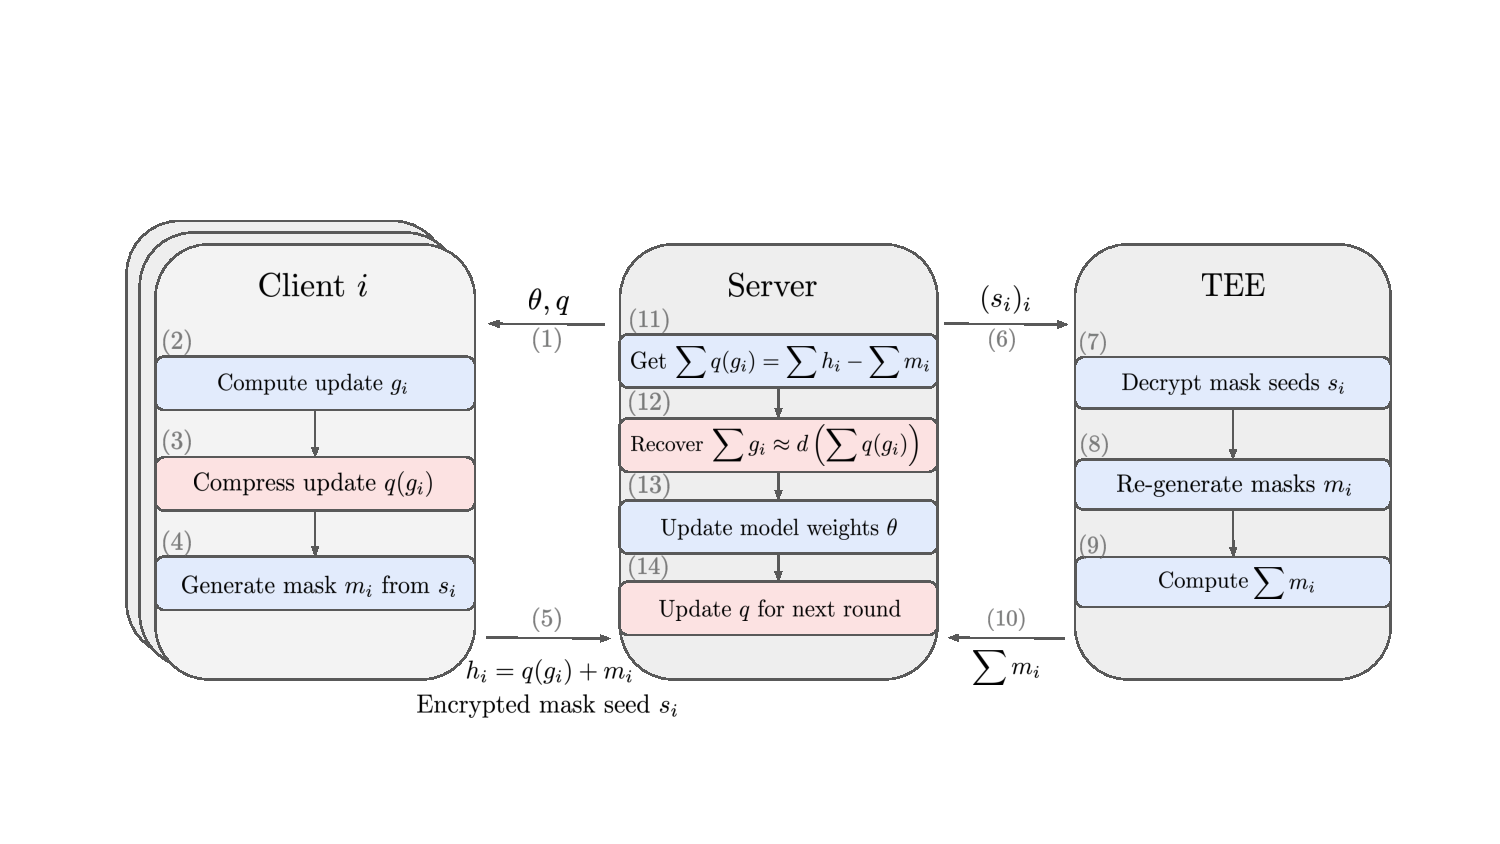
\includegraphics[width=0.9\textwidth]{submissions/GrahamCormode/figs/secagg_summary_new.pdf}
    %\vspace{-5mm}
    \caption{\label{fig:secagg_summary}
    Summary of the proposed approach for one FL round, where we omit the round dependency and \modif{Differential Privacy (DP)} for clarity. Blue boxes denote standard steps and red boxes denote additional steps for uplink compression. Client $i$ computes local model update $g_i$, compresses it with the compression operator $q$, and encrypts it by adding a random mask $m_i$ in the compressed domain, hence reducing the uplink bandwidth (steps 2--4). The server recovers the aggregate in the compressed domain by leveraging any \SecAgg protocol \modif{(steps 7--13, with a TEE-based \SecAgg, see Section~\ref{subsec:secagg})}. Since the decompression operator $d$ is linear, the server can convert the aggregate back to the non-compressed domain, up to compression error (step 12). As with the model weights $\theta$, the compression operator $q$ are also periodically updated and broadcast by the server (step 14).
    In Section~\ref{sec:method}, we apply the proposed method to scalar quantization and pruning without impacting \SecAgg and propose Secure Indexing, a variant of \SecAgg for extreme uplink compression with product quantization. See Section~\ref{subsec:secagg} for details about \SecAgg and Section~\ref{sec:discussion} for a discussion on~DP.
    }
    \vspace{-3mm}
\end{figure*}



% Our focus in this paper is on

%Second, scaling cross-device (synchronous) FL to millions of clients with various capabilities and intermittent availability \cite{Graham-bonavitz2019federated} suffers from diminishing returns: the wall-clock training time plateaus as the number of clients keeps increasing~\cite{Graham-huba2021papaya}. Even though this challenge can be addressed by leveraging the buffered asynchronous aggregation technique proposed by \cite{Graham-nguyen2021federated}, compatible with DP and SecAgg, the asynchronous protocol remains bottlenecked by communication latency between the server and the clients.


%Considering the above privacy and scalability goals, we focus on enabling efficient FL communications while keeping a high privacy bar. In addition to the primary objective of speeding up convergence, reducing communication costs brings other significant benefits. Lowering communication requirements addresses selection bias due to undersampling clients with limited connectivity, improving fairness and inclusivity metrics. Better communication efficiency shrinks the carbon footprint of FL, whose fraction attributable to communication can reach 95\%~\cite{Graham-qiu2021first}. %Finally, training larger model in FL would be a possibility, when the communication cost is reduced, because local memory or compute requirements can be addressed by modifying the local training loop, for instance with gradient checkpointing \cite{Graham-chen2016training}. However, some form of compression would be required to enable efficient communication.


%First, compressing model updates from the client to the server presents several challenges due to compatibility with SecAgg and is an area suitable for further research.
%Second, upload bandwidth is generally more restricted than download. For instance, according to the most recent FCC report, the ratio of download to upload speeds for DSL/cable providers in the US ranges between 3$\times$ to 20$\times$~\cite{Graham-fcc-broadband}. We consider broadband speeds here because devices participate in the FL training while connected to fixed broadband, usually through Wi-Fi~\cite{Graham-huba2021papaya}.




% Hence, FL provides the ability to leverage data from massive client populations while ensuring the security and privacy of the client data.
% Go further: compatibility with DP / compression as a mitigation techniques of attacks
% Model and gradient compression intrinsically different.
%  Why not having the secure enclave perform the aggregation?


\newcommand{\para}[1]{\noindent \textbf{#1}}

\section{Related Work}
\label{sec:related}

Communication is identified as a primary efficiency bottleneck in FL, especially in the cross-device FL setting~\cite{Graham-kairouz2019advances}.
This has led to significant interest in reducing FL's communication requirements. In what follows, we refer to a local model update in distributed training as a \emph{gradient}, including updates from multiple local training steps.

\para{Efficient Distributed Optimization.} There is a large body of literature on reducing the communication cost for distributed training. \cite{Graham-seide2014bit} proposes quantizing gradients to one bit while carrying the quantization error forward across mini-batches with error feedback. Similarly, \cite{Graham-wen2017terngrad} proposes layer-wise ternary gradients and \cite{Graham-bernstein2018signsgd} suggests using only the sign of the gradients. Gradient sparsity is another related area that is extensively studied \cite{Graham-wangni2017gradient,Graham-aji2017sparse,Graham-lin2017deep,Graham-renggli2018sparcml,Graham-parcollet2022zerofl}.
For instance, \cite{Graham-chen2017adacomp} and \cite{Graham-han2020adaptive} explore adapting the degree of sparsity to the distribution of local client data. Another method, QSGD, tunes the quantization level to trade possibly higher variance gradients for reduced communication bandwidth~\cite{Graham-alistarh2016qsgd}. Researchers also studied structured and sketched model updates \cite{Graham-konen2016federated}.
For example, \cite{Graham-wang2018atomo} proposes expressing gradients as a linear combination of basis vectors common to all workers and \cite{Graham-wang2022fedlite} propose to cluster the gradients and to implement error correction on the client side. Besides gradient compression, other methods such as~\cite{Graham-vepakomma2018split,Graham-hu2019dynamic} reduce the communication cost by partitioning the model such that each client learns a portion of it, while \cite{Graham-he2020group} proposes training small models and periodically distilling them to a larger central model. However, as detailed in Section~\ref{sec:background} and below, most of the proposed methods are not readily compatible with \SecAgg and cannot be used in secure FL.

\para{Bi-directional Compression.} In addition to uplink gradient compression, a line of work also focuses on downlink model compression. In a non-distributed setup, \cite{Graham-zhou2016dorefanet, Graham-courbariaux2015binaryconnect} demonstrates that it is possible to meaningfully train with low bit-width models and gradients. In FL, \cite{Graham-jiang2019model} proposes adapting the model size to the device to reduce both communication and computation overhead. Since the local models are perturbed due to compression, researchers propose adapting the optimization algorithm for better convergence \cite{Graham-liu2019double,Graham-sattler2019robust,Graham-tang2019doublesqueeze,Graham-zheng2019communicationefficient,Graham-amiri2020federated,Graham-philippenko2021preserved}.
Finally, pre-conditioning models during FL training can allow for quantized on-device inference, as demonstrated for non-distributed training by \cite{Graham-gupta2015deep, Graham-krishnamoorthi2018quantizing}. As stated in Section~\ref{sec:intro}, we do not focus on downlink model compression since uplink bandwidth is the main communication bottleneck and since \SecAgg only involves uplink communication.

\para{Aggregation in the Compressed Domain.} In the distributed setting, \cite{Graham-yu2018gradiveq} propose to leverage both gradient compression and parallel aggregation by performing the \emph{ring all-reduce} operation in the compressed domain and decompressing the aggregate. To do so, the authors exploit temporal correlations of the gradients to design a linear compression operator.
% Hence, the server receives the individual compressed gradients and is able to recover the sum of the non-compressed gradients:
% \[\sum_i q(g_i) = q\left(\sum g_i\right).\]
Another method, PowerSGD~\cite{Graham-vogels2019powersgd}, leverages a fast low-rank gradient compressor. However, both aforementioned methods are not evaluated in the FL setup and do not mention \SecAgg.
Indeed, the proposed methods focus on decentralized communication between the workers by leveraging the all-reduce operation.
Moreover, PowerSGD uses (stateful) error feedback on all distributed nodes, which is not readily adaptable to cross-device FL when clients generally participate in a few (not necessarily consecutive) rounds.
% not amenable to FL with SecAgg since the all-reduce operations requires communication between all distributed nodes and not solely through a central server.
Finally, \cite{Graham-rothchild2020fetchsgd} proposes FetchSGD, a compression method using sketching, which is compatible with \SecAgg.

% \ilya{Should we say that our methods are also variants of sketching?}
% \ilya{delete?}\st{In this paper, we focus on adapting standard compression methods to SecAgg (namely, scalar quantization and pruning) and propose Secure Indexing, a variant of SecAgg that is provably secure, to obtain extremely small model updates with product quantization.}





\newcommand{\parai}[1]{\noindent\textit{#1}}

\section{Background}
\label{sec:background}

In this section, we recall the \SecAgg protocol first, then the compression methods that we wish to adapt to \SecAgg, namely, scalar quantization, pruning, and product quantization.

\subsection{Secure Aggregation}
\label{subsec:secagg}

\SecAgg refers to a class of protocols that allow the server to aggregate client updates without accessing them individually. While \SecAgg alone does not entirely prevent client data leakage, it is a powerful and widely-used component of current at-scale cross-device FL implementations~\cite{Graham-kairouz2019advances}. Two main approaches exist in practice: software-based protocols relying on Multiparty Computation (MPC)~\cite{Graham-bonavitz2019federated,Graham-bell2020secure,Graham-LightSecAgg}, and those that leverage hardware implementations of Trusted Execution Environments (TEEs)~\cite{Graham-huba2021papaya}.
% While these approaches have substantial differences, they impose similar constraints on compatible update compression techniques: operating over finite fields and assuming that aggregation commutes with decompression.


\SecAgg relies on additive masking, where clients protect their model updates $g_i$ by adding a uniform random mask $m_i$ to it, guaranteeing that each client’s masked update is statistically indistinguishable from any other value.
% Masks are generated so that when all the masked client updates are aggregated by the server (typically through addition), the server obtains the exact aggregate (e.g., the sum of updates).
At aggregation time, the protocol ensures that all the masks are canceled out. For instance, in an MPC-based \SecAgg, the pairwise masks cancel out within the aggregation itself, since for every pair of users $i$ and $j$, after they agree on a matched pair of input perturbations, the masks $m_{i,j}$ and $m_{j,i}$ are constructed so that $m_{i,j}=-m_{j,i}$.
Similarly and as illustrated in Fig.~\ref{fig:secagg_summary}, in a TEE-based \SecAgg, the server receives $h_i = g_i + m_i$ from each client as well as the sum of the masks $\sum_i m_i$ from the TEE and recovers the sum of the updates as
% by unmasking the aggregated updates as
%\begin{equation*}
$
      \sum_i g_i = \sum_i h_i - \sum_i m_i.
$
%\end{equation*}
We defer the discussion of DP noise addition by \SecAgg protocols to Section~\ref{sec:discussion}.

\para{Finite Group.}
\SecAgg requires that the plaintexts---client model updates---be elements of a finite group, while the inputs are real-valued vectors represented with floating-point types.
This requirement is usually addressed by converting client updates to fixed-point integers and operating in a finite domain (modulo~$2^p$) where $p$ is typically set in prior literature to 32 bits. The choice of \SecAgg bit-width~$p$ must balance communication costs with the accuracy loss due to rounding and overflows.

% The other constraint is due to the fact that SecAgg is designed so that the server sees only the aggregate (the sum or the weighted sum) of individual gradients, plus some noise injected by a differentially private mechanism. A drop-in decompression operator $D$ must commute with SecAgg, or be close to being one:
% \[
% D\left(\sum_i g_i+\mathrm{noise}\right) \approx \sum_i D(g_i)+\mathrm{noise}.
% \]
\para{Minimal Complexity.}
\looseness=-1
TEE-based protocols offer greater flexibility in how individual client updates can be processed; however, the code executed inside TEE is part of the trusted computing base (TCB) for all clients. In particular, it means that this code must be stable, auditable, defects- and side-channel-free, which severely limits its complexity. Hence, in practice, we prefer compression techniques that are either oblivious to \SecAgg's implementation or require minimal changes to the TCB.

% In the remainder of the paper, we focus on the TEE-based approach for its simplicity, scalability and compatibility with asynchronous FL. relies on random masking to encrypt the local model updates. The server then incrementally aggregates the encrypted updates and unmasks the aggregate using the sum of the random masks transmitted by the Trusted Secure Aggregator (TSA) that sits within the TEE. More formally, let us denote $??$ a local client update, represented in floating-point precision, generally \texttt{fp32}. First, the client converts $??$ to a fixed point representation. Then, the client generates a random mask $m \in \Z^d$ and computes the sum modulo a number. \ashkan{TODO}

% SecAgg protocols prevent the server from accessing individual client updates by aggregating them and transmitting only the aggregate to the server. While such mechanisms alone do not entirely prevent data leakage, they constitute a vital component of cross-device FL implementations~\cite{Graham-kairouz2019advances}. SecAgg relies either on Secure Multiparty Computation \cite{Graham-bonavitz2019federated,so2021secure} or on a Trusted Executed Environment or TEE~\cite{Graham-huba2021papaya}. In the remainder of the paper, we focus on the TEE-based approach for its simplicity, scalability and compatibility with asynchronous FL.

% TEE-based SecAgg relies on random masking to encrypt the local model updates. The server then incrementally aggregates the encrypted updates and unmasks the aggregate using the sum of the random masks transmitted by the Trusted Secure Aggregator (TSA) that sits within the TEE. More formally, let us denote $??$ a local client update, represented in floating-point precision, generally \texttt{fp32}. First, the client converts $??$ to a fixed point representation. Then, the client generates a random mask $m \in \Z^d$ and computes the sum modulo a number.

% Since the server, by design, never observes

\subsection{Compression Methods}
\label{subsec:comp_methods}
In this subsection, we consider a matrix $W \in \mathbb{R}^{\cin\times \cout}$ representing the weights of a linear layer to discuss three major compression methods with distinct compression/accuracy tradeoffs and identify the challenges \SecAgg faces to be readily amenable to these popular quantization algorithms.

\subsubsection{Scalar Quantization}
\label{subsec:sq}

\looseness=-1 Uniform scalar quantization maps floating-point weight $w$ to $2^b$ evenly spaced bins, where $b$ is the number of bits. Given a floating-point scale $s > 0$ and an integer shift parameter $z$ called the zero-point, we map any floating-point parameter $w$ to its nearest bin indexed by $\{0,\dots, 2^b-1\}$:

\centerline{$w \mapsto \clamp(\round(w /s) + z, [0, 2^b - 1] ).$}

%
The tuple $(s, z)$ is often referred to as the quantization parameters (\texttt{qparams}).
With $b=8$, we recover the popular \texttt{int8} quantization scheme \cite{Graham-jacob2017quantization}, while setting $b = 1$ yields the extreme case of binarization \cite{Graham-courbariaux2015binaryconnect}.
The quantization parameters $s$ and $z$ are usually calibrated after training a model with floating-point weights using the minimum and maximum values of each layer.
% The accuracy drop due to this post-training quantization can be mitigated by pre-conditioning the network during training with techniques such as Quantization-Aware Training or QAT~\cite{Graham-krishnamoorthi2018quantizing}.
% The quantization parameters can also be defined per-channel instead of per-layer to diminish the quantization error at the cost of a small memory overhead.
The compressed representation of weights $W$ consists of the \texttt{qparams} and the integer representation matrix $W_q$ where each entry is stored in~$b$~bits.
Decompressing any integer entry $w_q$ of~$W_q$ back to floating point is performed by applying  the (linear) operator $w_q \mapsto s\times(w_q - z)$.

\para{Challenge.}
The discrete domain of quantized values and the finite group required by \SecAgg are not natively compatible because of the overflows that may occur at aggregation time. For instance, consider the extreme case of binary quantization, where each value is replaced by a bit.
We can represent these bits in \SecAgg with $p=1$, but the aggregation will inevitably result in overflows.

\subsubsection{Pruning}
\label{subsec:rp}

Pruning is a class of methods that remove parts of a model such as connections or neurons according to some pruning criterion, such as weight magnitude~(\cite{Graham-lecun1990optimal,Graham-hassabi1992second}; see \cite{Graham-Blalock20} for a survey). \cite{Graham-konen2016federated} demonstrate client update compression with random sparsity for federated learning. Motivated by previous work and the fact that random masks do not leak information about the data on client devices, we will leverage random pruning of client updates in the remainder of this paper.
% as it is easiest to combine with SecAgg.
% Let $\texttt{rand}$ be a function generating random entries in interval $[0, 1)$.
% For a sparsity level $0\leq\rho\leq 1$, where $\rho=1$ yields a zero matrix, a client prunes entries~$w$ of~$W$ as:
% % \karthik{TODO: decide on notation for rand}
% \[w \mapsto \begin{cases}
% 0 & \text{if } \texttt{rand()} < \rho \\
% w & \text{otherwise}.
% \end{cases}
% \]
% \sayan{should we number the equations ?}
A standard method to store a sparse matrix is the coordinate list (COO) format\footnote{See the  {torch.sparse documentation}, \url{https://pytorch.org/docs/stable/sparse.html}.}, where only the non-zero entries are stored (in floating point or lower precision), along with their integer coordinates in the matrix.
This format is compact, but only for a large enough compression ratio, as we store additional values for each non-zero entry.
Decompression is performed by re-instantiating the uncompressed matrix with both sparse and non-sparse entries.

\para{Challenge.}
\modif{Pruning model updates on the client side is an effective compression approach} as investigated in previous work. However, the underlying assumption is that clients have different masks, either due to their seeds or dependency on client update parameters (\eg weight magnitudes). This is a challenge for \SecAgg as aggregation assumes a dense compressed tensor, which is not possible to construct when the coordinates of non-zero entries are not the same for all clients.

\subsubsection{Product Quantization}
\label{subsec:pq}


Product quantization (PQ) is a compression technique developed for nearest-neighbor search \cite{Graham-jegou2011product} that can be applied for model compression \cite{Graham-stock2019bit}.
Here, we show how we can re-formulate PQ to represent model updates.
We focus on linear layers and refer the reader to~\cite{Graham-stock2019bit} for adaptation to convolutions.
Let the \emph{block size} be $d$ (say, 8), the number of \emph{codewords} be $k$ (say, 256) and assume that the number of input channels, $\cin$, is a multiple of $d$.
To compress $W$ with PQ, we evenly split its columns into subvectors or blocks of size $d \times 1$ and learn a \emph{codebook} via $k$-means to select the $k$ codewords used to represent the $\cin\times\cout/d$ blocks of $W$. PQ with block size $d=1$ amounts to non-uniform scalar quantization with $\log_2 k$ bits per weight.
% More formally, we first reshape $ W$ into a matrix of size $d \times \cin \cout / d$ and with a slight abuse of notation, we will also use  $W$ to denote the reshaped matrix and work only in the reshaped space.
% Note that the reshaping approach applies to convolutional weights as well: e.g., for a 2D convolution with a kernel of size of $k_s$, we need to change the reshaping part to get matrix of size $d \times \cin\cout k_s^2/d$.

The PQ-compressed matrix $W$ is represented with the tuple $(C, A)$, where $C$ is the codebook of size $k \times d$ and $A$ gives the assignments of size $\cin \times\cout / d$.
% \begin{align*}
% C & \text{    the codebook of size } k \times d,  \\
% A & \text{    the assignments of size }\cin \cdot\cout / d.
% \end{align*}
Assignments are integers in $[0, k-1]$ and denote which codebook a subvector was assigned~to.
To decompress the matrix (up to reshaping), we index the codebook with the assignments, written in PyTorch-like notation as
%\begin{equation*}
$
    \widehat {W} = C[A].
$
%\end{equation*}
% (appropriating a PyTorch-like notation) and perform a reshaping operation. PQ is naturally extensible to convolutional layers~\cite{Graham-stock2019bit}.

\para{Challenge.}
There are several obstacles to making PQ compatible with \SecAgg.
First, each client may have a different codebook, and direct access to these codebooks is needed to decode each client's message.
Even if all clients share a (public) codebook, the operation to take assignments to produce an (aggregated) update is not linear, and so cannot be directly wrapped inside \SecAgg.
%In theory PQ is a linear operation, since we can encode each client's choice of codeword for a block with a 1-hot vector of length $k$, and com



\section{Method}
\label{sec:method}

In this section, we propose solutions to
% the challenges identified in Section~\ref{subsec:comp_methods} to
reconcile security (\SecAgg) and communication efficiency.
Our approach is to modify compression techniques to share some hyperparameters globally across all clients so that aggregation can be done by uniformly combining each client's response, while still ensuring that there is scope to achieve accurate compressed representations.
\modif{As detailed below, each of the proposed methods offers the same level of security as standard \SecAgg without compression.}

\subsection{Secure Aggregation and Compression}
\label{subsec:secagg_comp}
We propose to compress the uplink model updates through a compression operator $q$, whose parameters are round-dependent but the same for all clients participating in the same round.
Then, we will add a random mask $m_i$ to each quantized client update $q(g_i)$ in the compressed domain, thus effectively reducing uplink bandwidth while ensuring that $h_i = q(g_i) + m_i$ is statistically indistinguishable from any other representable value in the finite group (see Section~\ref{subsec:secagg}).
In this setting, \SecAgg allows the server to recover the aggregate of the client model updates in the compressed domain: $\sum_i q(g_i)$.
% \begin{equation*}
%     \sum_i q(g_i) = \sum_i h_i- \sum_i m_i
% \end{equation*}
If the decompression operator $d$ is linear, the server is able to recover the aggregate in the non-compressed domain, up to quantization error, as illustrated in Figure~\ref{fig:secagg_summary}:
\begin{equation*}\textstyle
    d\left(\sum_i h_i - \sum_i m_i\right) = d\left(\sum_i q(g_i)\right) =\sum_i d(q(g_i)) \approx \sum_i g_i.
\end{equation*}
% \ashkan{according to the top equation in page 4, $\sum h_i$ minus $\sum m_i$ is exactly $\sum g_i$ and not $\sum q(g_i)$. I understand here we are talking about compression. But a reviewer might complain here that this is not consistent. Should we add $q(.)$ around the first part too?}
The server periodically updates the quantization and decompression operator parameters, either from the aggregated model update, which is deemed public, or by emulating a client update on some similarly distributed public data. Once these parameters are updated, the server broadcasts them to the clients for the next round. \modif{This adds overhead to the downlink communication payload, however, this is negligible compared to the downlink model size to transmit}. For instance, for scalar quantization, $q$ is entirely characterized by one \texttt{fp32} scale and one \texttt{int32} zero-point per layer, the latter of which is unnecessary in the case of a symmetric quantization scheme. Finally, this approach is compatible with both synchronous FL methods such as FedAvg~\cite{Graham-mcmahan2016communicationefficient} and asynchronous methods such as FedBuff~\cite{Graham-nguyen2021federated} as long as \SecAgg maintains the mapping between the successive versions of quantization parameters and the corresponding client updates.

\subsection{Application}
Next, we show how we adapt scalar quantization and random pruning with no changes required to \SecAgg. We illustrate our point with TEE-based \SecAgg while these adapted uplink compression mechanisms are agnostic of the \SecAgg mechanism. Finally, we show how to obtain extreme uplink compression by proposing a variant of \SecAgg, which we call \SecInd. This variant supports product quantization and is provably secure.

\subsubsection{Scalar Quantization and Secure Aggregation}
\label{subsubsec:sq_sa}

As detailed in Section~\ref{subsec:sq}, a model update matrix $g_i$ compressed with scalar quantization is given by an integer representation in the range $[0, 2^{b}-1]$ and by the quantization parameters \emph{scale} ($s$) and \emph{zero-point} ($z$). A sufficient condition for the decompression operator to be linear is to broadcast common quantization parameters per layer for each client. Denote $q(g_i)$ as the integer representation of quantized client model update $g_i$ corresponding to a particular layer for client $1\leq i \leq N$.
%Let us assume that the server's aggregation method is the sum.
Set the scale of the decompression operator to $s$ and its zero-point to $z/N$.
Then, the server is able to decompress as follows (where the decompression operator is defined in Section~\ref{subsec:sq}):
\begin{equation*}\textstyle
    % (s\sum_i  q(g_i)) - \frac{sz}{n} = \sum_i s(q(g_i) - z) \simeq \sum_i g_i.
    d\left(\sum_i q(g_i)\right) = s\sum_i  q(g_i) -  \frac{z}{N}  = \sum_i \left( s(q(g_i)) - z \right) \approx \sum_i g_i
\end{equation*}
Recall that all operations are performed in a finite group. Therefore, to avoid overflows at aggregation time, we quantize with a bit-width $b$ but take \SecAgg bit-width $p > b$, thus creating a margin for potential overflows (see Section~\ref{subsec:ablations}).
%\ilya{Do we really? (Make SecAgg bitwidth larger than b.) Masked updates are defined only modulo $2^b$, adding them in larger group makes little sense.}.
%
This approach is related to the fixed-point aggregation described in \cite{Graham-bonavitz2019federated,Graham-huba2021papaya}, but we calibrate the quantization parameters and perform the calibration per layer and periodically, unlike the related approaches.
% whereas the scale parameter used in fixed-point conversion does not change during the training and is common to the whole network.\ilya{I am confused - does the scale change periodically or it doesn't?}

\modif{\para{Privacy, Security and Bandwidth.}} Scales and zero points are determined from public data on the server. Downlink overhead is negligible: the server broadcasts the per-layer quantization parameters. The upload bandwidth is $p$ bits per weight, where $p$ is the \SecAgg finite group size (Section~\ref{subsec:secagg}). \modif{Since the masks $m_i$ are chosen in the integer range $[0, 2^p-1]$, any masked integer representation taken modulo $2^p$ is statistically indistinguishable from any other vector.}
% The maximum ``price of security'' is thus the overflow buffer of $p-b = \lceil\log_2 N\rceil$ bits per weight.

\subsubsection{Pruning and Secure Aggregation}

To enable linear decompression with random pruning, all clients will share a common pruning mask for each round.
This can be communicated compactly before each round as a seed for a pseudo-random function.
%the server broadcasts one common pruning mask seed before each round.
This pruning mask seed is different from the \SecAgg mask seed introduced in Section~\ref{subsec:secagg} and has a distinct role.
Each client uses the pruning seed to reconstruct a pruning mask, prunes their model update $g_i$, and only needs to encrypt and transmit the unpruned parameters.
The trade-off here is that some parameters are completely unobserved in a given round, as opposed to traditional pruning.
%we obtain no signal about some parameters in a given round, in contrast to traditional pruning.
\SecAgg operates as usual and the server receives the sum of the tensor of unpruned parameters computed by participating clients in the round, which it can expand using the mask seed.
We denote the pruning operator as $\phi$ applied to the original model update $g_i$, and the decompression operator as $d$ applied to a compressed tensor $\phi(g_i)$. Decompression is an expansion operation equivalent to multiplication with a sparse permutation matrix $P_i$ whose entries are dependent on the $i$'th client's mask seed.
Crucially, when all clients share the same mask seed within each round, we have $P_i = P$ for all $i$ and linearity of decompression is maintained:
\begin{equation*} \textstyle
    d \left(\sum_i \phi(g_i) \right) = P \left( \sum_i \phi(g_i) \right) = \sum_i P_i\phi(g_i) = \sum_i d(\phi(g_i)) \approx \sum_i g_i.
\end{equation*}
%
\modif{\para{Privacy, Security and Bandwidth.}} Since the mask is random, no information leaks from the pruning mask. The downlink overhead (the server broadcasts one integer mask seed) is negligible. The upload bandwidth is simply the size of the sparse client model updates. \modif{Finally, there is no loss in security since each client uses standard \SecAgg mechanism on the non-pruned entries.}

\subsubsection{Product Quantization and Secure Indexing}

\begin{algorithm}[t]
\caption{Secure Indexing (\SecInd)}
\label{alg:sec_indexing}
\begin{algorithmic}[1]

% \Procedure{On client}{C}      \Comment{Client-side logic}
%     \State Receive common codebook $C$
%     \State Compute assignment matrix $A^i$  \Comment{$i$ is the client index}
%     \State Encrypt assigment matrix \Comment{For instance with additive masking}
% \EndProcedure

\Procedure{SecureIndexing}{C}      \Comment{This happens inside the TEE}
    \State Receive common codebook $C$ from server \Comment{$C$ is periodically updated by the server}
    \State Initialize histograms $H_{m,n}$ to $0$ \Comment{Each histogram for block $(m, n)$ has size $k$}
    \For{each client $i$}
    \State Receive and decrypt assignment matrix $A^i$ %\Comment{For instance with additive masking}
        \For{each block index $(m, n)$}
            \State $r \leftarrow A^i_{m, n}$ \Comment{Recover assignment of client $i$ for block $(m, m)$}
            \State $H_{m, n}[r] \leftarrow H_{m, n}[r] + 1$ \Comment{Update global count for codeword index $r$}
        \EndFor
    \EndFor
    \State Send back histograms $H_{m, n}$ to the server
\EndProcedure
\end{algorithmic}
\end{algorithm}



% \ashkan{question on notatin: sometimes we have () around A, sometimes we do not, e.g. in the equation below. Sometimes the superscript $i$ is outside () and sometimes inside. Do these have different meaning?}
% We first express product quantization in terms of a linear decompression operator.
%We describe the novel Secure Indexing protocol


We next describe the Secure Indexing (\SecInd) primitive, and discuss how to instantiate it.
Recall that with PQ, each layer has its own codebook $C$ as explained in Section~\ref{sec:method}.
Let us fix one particular layer compressed with codebook $C$, containing $k$ codewords.
We assume that $C$ is common to all clients participating in the round.
Consider the assignment matrix of a given layer $(A^i)_{m,n}$ for client~$i$.
From these, we seek to build the \emph{assignment histograms} $H_{m,n} \in \mathbb R^k$ that satisfy
%\begin{equation*}
$H_{m,n}[r] = \sum_i \mathbf 1\left(A^i_{m,n} = r\right),$
%\end{equation*}
where the indicator function $\mathbf 1$ satisfies $\mathbf 1\left(A^i_{m,n} = r\right) = 1$ if $A^i_{m,n} = r$ and $0$ otherwise.
A \emph{Secure Indexing} primitive will produce~$H_{m,n}$ while ensuring that no other information about client assignments or partial aggregations is revealed.
The server receives assignment histograms from \SecInd and is able to recover the aggregated update for each block indexed by $(m, n)$ as
%\begin{equation*}
$
        \sum_r  H_{m,n}[r] \cdot C[r].
$
%\end{equation*}
%
We describe how \SecInd can be implemented with a TEE in Algorithm~\ref{alg:sec_indexing}.
Each client encrypts the assignment matrix, for instance with additive masking as described in Section~\ref{subsec:secagg}, and sends it to the TEE via the server.
Hence, the server does not have access to the plaintexts client-specific assignments.
TEE decrypts each assignment matrix and for each block indexed by $(m, n)$ produces the assignment histogram.
%\ilya{sentence fragment. I don't know where it is heading.}
% where
% \begin{equation*}
%     \mathbf 1\left(A^i_{m,n} = r\right) =
%     \begin{cases}
%         1 & \text{if } A^i_{m,n} = r  \\
%         0  & \text{otherwise}.
%     \end{cases}
% \end{equation*}
%\ilya{Delete:}\st{Since the enclave decrypts the individual assignment matrices, the proposed method is orthogonal to the encryption process.}
Compared to \SecAgg, where the TEE receives an encrypted seed per client (a few bytes per client) and sends back the sum of the masks $m_i$ (same size as the considered model), \SecInd receives the (masked) assignment matrices and sends back histograms for each round.
%\SecInd implementation feasibility is briefly discussed in Appendix~\ref{appendix:secind}.
\SecInd can be implemented in other models, offering different trust paradigms,
such as the multi-party computation setting (using two or more servers to operate on shares of the input).
Encoding inputs as shares of one-hot vectors would lose the advantages of compression.
Instead, each client can send evaluations of \emph{distributed point functions} to encode each assignment~\cite{Graham-boyle16}.
These are represented compactly, but may require longer codewords to overcome the overheads.

%An advantage of working with multiple servers is that we can compute the final output (\ie the update) without exposing any intermediate representation in terms of the histogram of codewords.
%That is, we could obtain shares of the histogram in the MPC model, and then use these in conjunction with the (public) codebook to build shares of the update, before finally combining these to reveal the update.
%This could also be combined with the introduction of DP noise to ensure privacy as well as security.
% expands it to $(\widetilde A^i)_{m,n,r}$ by replacing each assignment index by a one-hot vector of size $k$:
% \[  \widetilde A^i_{m,n,r} =
%     \begin{cases}
%         1 & \text{if } A^i_{m,n} = r  \\
%         0  & \text{otherwise}.
%     \end{cases}
% \]
% Let us assume further that the codebook $C$ is common to all clients participating in the round.
% % $C$ is computed by the server
% % %on a mock client
% % using public data or from the aggregated (public) model update.
% Then, the server is able to recover the aggregated update for each block indexed by $(m, n)$:
% \[ \ashkan{?=}\sum_r \left(\sum_{i} \widetilde A^i_{m,n,r} \right)\cdot C_r
% \]
% However, in practice we do not wish to instantiate the sparse matrix $(\widetilde A^i)_{m,n,r}$ due to its size.
% Instead, we propose Secure Indexing\karthik{where exactly do we propose this?}, a variant of SecAgg that receives the (non-expanded) assignment matrices $(A)^i_{m,n}$ and sends the aggregate back to the server in a compact form.



\modif{\para{Privacy, Security and Bandwidth.}}
Codebooks are computed from public data while individual assignments are never revealed to the server.
The downlink overhead of sending the codebooks is negligible as demonstrated in Section~\ref{sec:experiments}.
The upload bandwidth in the TEE implementation is the assignment size, represented in $k$ bits (the number of codewords).
For instance, with a block size $d=8$ and $k=32$ codewords, assignment storage costs are 5 bits per 8 weights, which converts to 0.625 bits per weight.
The tradeoff compared to non-secure PQ is the restriction to a global codebook for all clients (instead of one tailored to each client), and the need to instantiate \SecInd instead of \SecAgg. \modif{Since the assignments are encrypted before being sent to the TEE, there is no loss in security. Here, any encryption mechanism (not necessarily relying on additive masking) would work.}


\section{Experiments}
\label{sec:experiments}

\begin{figure*}[t]
    \centering
    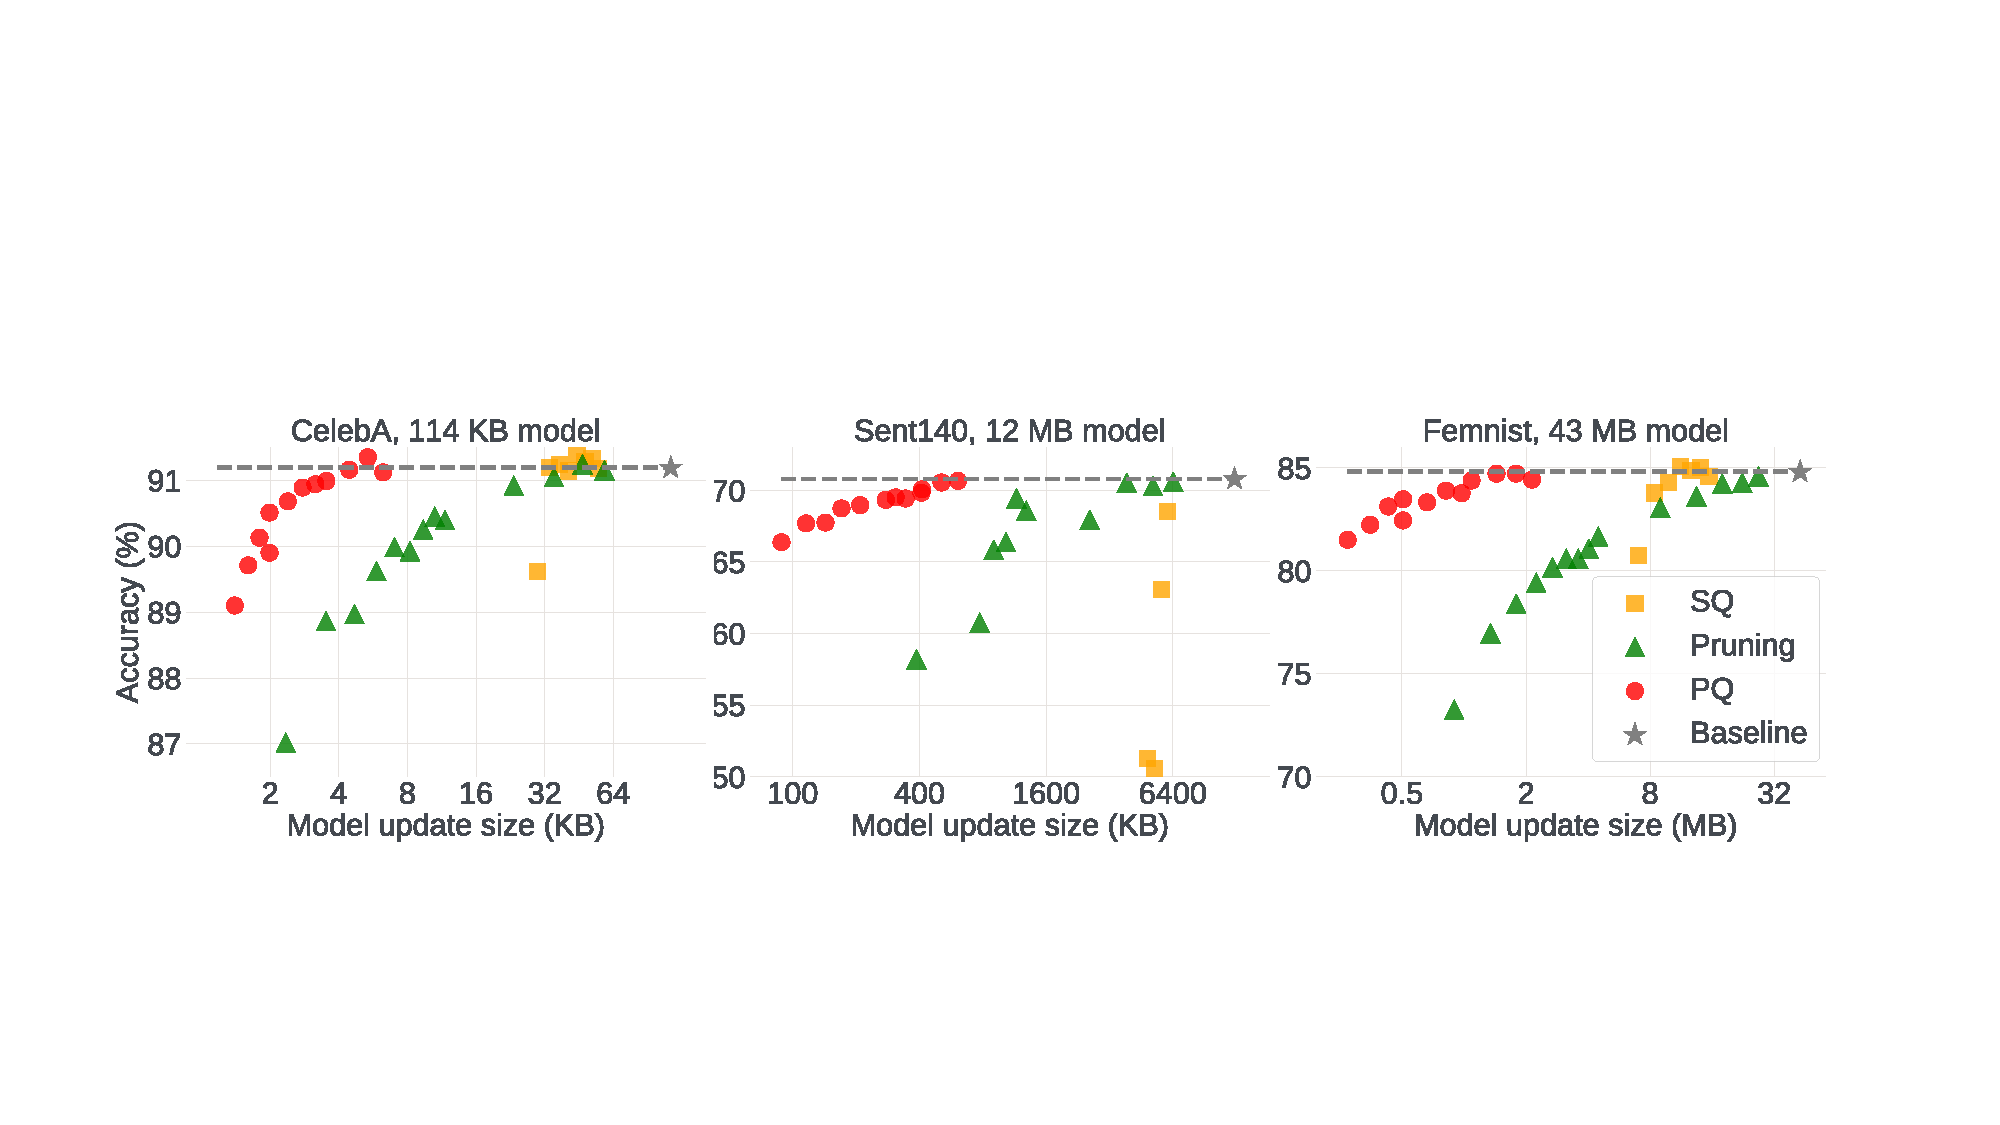
\includegraphics[width=\textwidth]{submissions/GrahamCormode/figs/results_summary.pdf}
    \vspace{-5mm}
    \caption{\label{fig:results_summary}
    We adapt scalar quantization (SQ) and pruning to the \SecAgg protocol to enable efficient and secure uplink communications. We also present results for product quantization (PQ) under the proposed novel \SecInd protocol. \modif{\emph{The $x$ axis is log-scale} and represents the uplink message size}. Baseline refers to \SecAgg FL run without any uplink compression, shown as a horizontal line for easier comparison. Model size is indicated in plot titles. Uncompressed client updates are as large as the models when $p=32$ (see Sec~\ref{subsec:secagg}, shown as stars).
    %We refer to the Appendix~\ref{appendix:table} for the matching tables where we additionally report the standard deviation of each data point.
    }
\end{figure*}

% \pierre{TODO: Table/graph for SQ overflows}
% \pierre{Convergence curves baseline vs compression?}
%In this section, w
We evaluate the performance of the proposed approaches when adapted to \SecAgg protocols.
We study the relationship between uplink compression and model accuracy for the LEAF benchmark tasks.
For scalar and product quantization we also analyze the impact of refresh rate for compression parameters on  model performance.

\subsection{Experimental Setup}
\label{subsec:setup}
We follow the setup of~\cite{Graham-nguyen2021federated} and use the {FLSim library}
% \footnote{Available at \href{https://github.com/facebookresearch/FLSim}{https://github.com/facebookresearch/FLSim}}
for our experiments
% \footnote{Code available at \texttt{github.com/facebookresearch/SecureFLCompression}.}
.
All experiments are run on a single V100 GPU 16 GB (except for Sent140 where we use one V100 32 GB) and typically take a few hours to run.
%More experiment details can be found in Appendix \ref{appendix:exp_details}.

\para{Tasks.} We run experiments on three datasets from the LEAF benchmark~\cite{Graham-caldas2018leaf}: CelebA~\cite{Graham-liu2015faceattributes}, Sent140~\cite{Graham-Go_Bhayani_Huang_2009} and FEMNIST~\cite{Graham-lecun2010mnist}. For CelebA, we train the same convolutional classifier as ~\cite{Graham-nguyen2021federated} with BatchNorm layers replaced by GroupNorm layers and 9,343 clients. For Sent140, we train an LSTM classifier for binary sentiment analysis with $59,400$ clients.
For FEMNIST, we train a GroupNorm version of the ResNet18~\cite{Graham-he2015deep} for digit classification with 3,550 clients.
We do not compress biases and norm layers due to their small overhead.

\para{Baselines.}  We focus here on the (synchronous) FedAvg approach although, as explained in Section~\ref{sec:method}, the proposed compression methods can be readily adapted to asynchronous FL aggregation protocols. \modif{As in prior work, we keep the number of clients per round to at most $100$,
%(see Appendix~\ref{appendix:exp_details}),
a small fraction of the total considered population size~\cite{Graham-chen2019federated,Graham-charles2021largecohort}.}
We report the average and standard deviation of accuracy over three independent runs for all tasks at different uplink byte sizes corresponding to various configurations of the compression operator.
% \sayan{important point : why do we use gradient and client update interchangeably ? they're not the same and for FedAvg it should be client update deltas ?} \karthik {I belieev I have changed gradients to client updates everywhere, except in related works section where we warn we might use graidents to mean updates}

% \subsection{Secure and Efficient Uplink Communications}

\para{Implementation Details.} We refer the reader to \cite{Graham-techreport} for full experiment details.
The downlink overhead of sending the per-layer codebooks for product quantization is negligible.
%as shown in Appendix~\ref{appendix:codebook_size}.
The convergence time in terms of rounds is similar for PQ runs and the non-compressed baseline/
%, as illustrated in Appendix~\ref{appendix:convergence}.
Note that outside a simulated environment, the wall-clock time convergence for PQ runs would be \emph{lower} than the baseline since uplink communication would be more efficient, hence faster.

\subsection{Results and Comparison with Prior Work}

Results for efficient and secure uplink communications are displayed in Figure~\ref{fig:results_summary}.
%Note that each method is either design to be adapted to S\SecAgg
We observe that PQ yields a consistently better trade-off curve between model update size and accuracy. For instance, on CelebA, PQ achieves $\times 30$ compression with respect to the non-compressed baseline at iso-accuracy. The iso-accuracy compression rate is $\times 32$ on Sent140 and $\times 40$ on FEMNIST (see~\cite{Graham-techreport} for detailed tables).
Scalar quantization accuracy degrades significantly for larger compression rates due to the overflows at aggregation.
%as detailed in Appendix~\ref{appendix:overflow}.
Pruning gives intermediate tradeoffs between scalar quantization and product quantization.

The line of work that develops FL compression techniques is exemplified by FetchSGD~\cite{Graham-rothchild2020fetchsgd} as detailed in Section~\ref{sec:related}, where the authors do not address \SecAgg.
Their results are not directly comparable to ours due to incomparable experimental setups (e.g., datasets and architectures).
However, Figure 6~\cite{Graham-techreport} mentions upload compression rates at iso-accuracy that are weaker than those obtained here with product quantization.

\subsection{Ablation Studies}
\label{subsec:ablations}

\begin{figure*}[t]
    \label{mask-refresh}
    \centering
    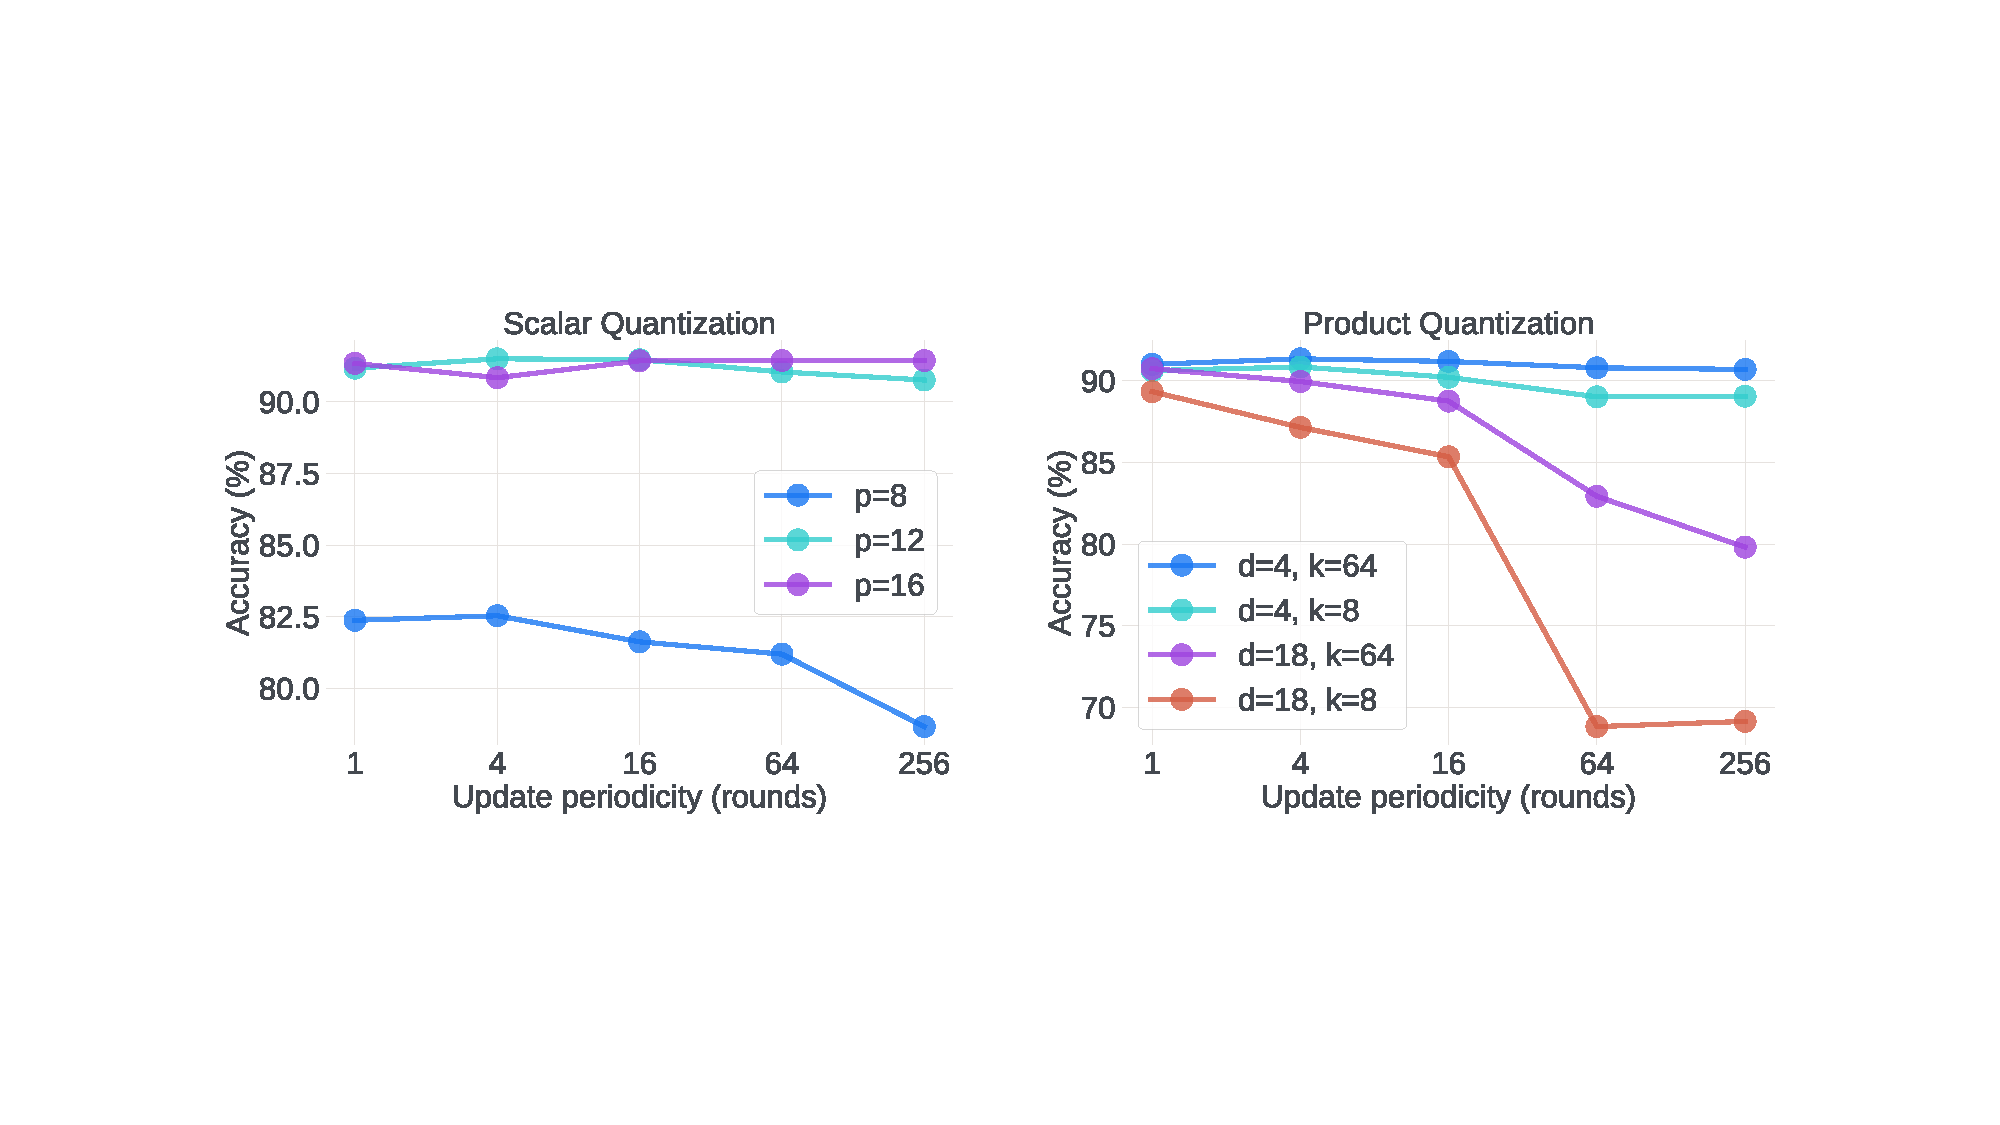
\includegraphics[width=0.9\textwidth]{submissions/GrahamCormode/figs/refresh.pdf}
    \caption{\label{fig:refresh}
    Impact of the refresh rate of the compression operator by the server on the CelebA dataset. \textbf{Left}:  scalar quantization (quantization parameters), fixing the quantization bit-width $b=8$ ($p$ denotes the \SecAgg bit-width). \textbf{Right}: for product quantization (codebooks), where $k$ denotes the number of codewords and $d$ the block size.}
    \vspace{-3mm}
\end{figure*}


We investigate the influence of the frequency of updates of the compression operator $q$ for scalar quantization and pruning, and study the influence of the \SecAgg bit-width $p$ on the number of overflows for scalar quantization.

\para{Update frequency of the compression operators.} In Figure~\ref{fig:refresh}, we show that for scalar quantization, the update periodicity only plays a role with low \SecAgg bit-width values $p$ compared to the quantization bit-width $b$. For product quantization, the update periodicity plays an important role for aggressive compression setups corresponding to large block sizes $d$ or to a smaller number of codewords $k$. For pruning, we measure the impact of masks that are refreshed periodically.
We observed that if we refresh the compression operator more frequently, staleness is reduced, leading to accuracy improvements.
%We present our findings in Appendix~\ref{sparse_refresh}.

\para{Overflows for scalar quantization.}
As discussed in Section~\ref{subsubsec:sq_sa}, we choose the \SecAgg bit-width~$p$ to be greater than quantization bit-width~$b$ in order to avoid aggregation overflows. While it suffices to set $p$ to be $\lceil\log_2 n_c\rceil$ more than $b$, where $n_c$ is the number of clients participating in the round, reducing $p$ is desirable to reduce uplink size.
We studied the impact of  $p$ on the percentage of parameters that suffer overflows, and
observed that there is a benefit to having some non-zero overflow margin size, but no clear correlation between margin size and accuracy.
%present our findings in Appendix~\ref{appendix:overflow}.

% \para{Update frequency of pruning operator $\varrho$.}

% \begin{table*}[t]
%     \small
%     \centering
%     % \vspace{3pt}
%     \begin{tabular}{l@{\hspace{20pt}} c ccc cl@{\hspace{20pt}} ccc}
%     \toprule
%  \bf Compression Method &~~& \multicolumn{3}{c}{\bf CelebA} &~~& \multicolumn{3}{c}{\bf Sent140}\\
%  && \multicolumn{3}{c}{\small ResNet18} &~~& \multicolumn{3}{c}{\small LSTM}\\
% %  && \multicolumn{3}{c}{\small Wikitext-103} &~~& \multicolumn{3}{c}{\small ImageNet-1k}\\
% \cmidrule{3-5}
% \cmidrule{7-9}
% && Gradient size & Compression & Top-1 && Gradient Size & Compression & PPL \\
%     \midrule
%     Baseline & &  $-$ & $\times\ \ 1$ & $-$ & &  $-$ & $\times\ \ 1$ & $-$   \\
%     % \midrule
%     % Binarization & & \\
%     % + \method & & \\
%     \midrule
%     SQ (8 bits) & &  $-$ & $\times\ \ -$ & $-$ & &  $-$ & $\times\ \ -$ & $-$   \\
%     SQ (4 bits) & &  $-$ & $\times\ \ -$ & $-$ & &  $-$ & $\times\ \ -$ & $-$   \\
%     \midrule
%     Pruning ($s=90\%$) & &  $-$ & $\times\ \ -$ & $-$ & &  $-$ & $\times\ \ -$ & $-$   \\
%     Pruning ($s=50\%$) & &  $-$ & $\times\ \ -$ & $-$ & &  $-$ & $\times\ \ -$ & $-$   \\
%     Pruning ($s=10\%$) & &  $-$ & $\times\ \ -$ & $-$ & &  $-$ & $\times\ \ -$ & $-$   \\
%     \midrule
%     PQ ($k=256$, $d=4$) & &  $-$ & $\times\ \ -$ & $-$ & &  $-$ & $\times\ \ -$ & $-$   \\
%     PQ ($k=256$, $d=8$) & &  $-$ & $\times\ \ -$ & $-$ & & $-$ &  $\times\ \ -$ &  $-$  \\
%     \bottomrule
%     \end{tabular}
%  \caption{\small \textbf{Comparison of different quantization schemes with Secure Aggregation}. Blabla.}
%     \label{tab:quantization_comparison}
% \end{table*}


% \subsection{Combination of Compression Techniques}

% \pierre{Song Han Deep Compression for combination}

% \subsubsection{Sparsity \& Scalar Quantization}
% Say/demonstrate that its better to perform pruning first and then SQ than the opposite.

% \subsubsection{Sparsity \& Product Quantization}
% Block sparsity and PQ.

% \subsection{FL Finetuning}

% Maybe also talk about the realistic scenario of FL finetuning (in practice, start from pretrained model on public data to bootstrap learning, in which case gradients may be smaller/sparser hence easier to compress?).
% Partial finetuning.

% \subsection{Heterogeneous Hardware}

% Experiment describing various bit-widths/sparsity level/codebook size per client depending on available bandwidth.

% \pierre{delta with respect to baseline}
% \pierre{discussion about privacy of shared parameters}
% \pierre{DP noise in the enclave until the very end. Privacy vs security = secure FL focus}
% \pierre{Secure Coding}


\section{Concluding Remarks}
\label{sec:discussion}
In this paper, we reconcile efficiency and security for uplink communication in Federated Learning.
We propose to adapt existing compression mechanisms such as scalar quantization and pruning to the secure aggregation protocol by imposing a linearity constraint on the decompression operator.
Our experiments demonstrate that we can adapt both quantization and pruning mechanisms to obtain a high degree of uplink compression with minimal degradation in performance and higher security guarantees. For achieving the highest rates of compression, we introduce \SecInd, a variant of \SecAgg well-suited for TEE-based implementation that supports product quantization while maintaining a high security bar.
%We plan to extend our work to other federated learning scenarios, such as asynchronous FL, and further investigate the interaction of compression and privacy.
%\section{Extensions}
As mentioned in Section~\ref{sec:intro}, we {may want } both \SecAgg and Differential Privacy~\cite{Graham-abadi2016deep} to realize the full promise of FL as a privacy-enhancing technology.
While our primary focus is on enabling efficient and secure uplink communication, we emphasize that the proposed approaches are compatible with user-level DP.
For instance, {at the cost of increasing the complexity of the trusted computing base}, DP noise can be added natively by the TEE with our modified random pruning or scalar quantization approaches.
For PQ  and \SecInd, {we can have the TEE to add noise in the assignment space (\ie outputting a noisy histogram), or to map the histogram to the codeword space and add noise there.
Each option offers a different tradeoff between privacy, trust, and accuracy; we leave detailed evaluation to future work.}




%\modif{\textbf{Compatibility with DP.}
%\sout{it would require, however, to transfer the aggregation to TEE or to design a DP mechanism in the assignment space, since DP noise must be added by the TEE and not by the server.}}

%\modif{\textbf{Efficiency and Privacy.}} A separate line of work {aims} to combine communication efficiency and privacy.
%For instance, \cite{Graham-triastcyn2021dprec} develop a method that unifies compressed communication and DP (where integration with \SecAgg is left as an open problem), while \cite{Graham-chaudhuri2022privacyaware} design a privacy-aware scalar compression mechanism within the \emph{local} differential privacy model.

%\graham{\sout{
%\modif{\textbf{Broader Social Impact. }} In this work, we propose to enhance the privacy of individuals who may contribute to training ML models and simultaneously enable more individuals to participate in private training, who might otherwise have been excluded due to resource constraints. }}
% Indeed, Federated Learning could enable a malicious server to access individual model updates that can leak personal information. Hence, we propose a secure way to communicate the individual model updates.

% - Generic and less data-dependent codebook
% - Model compression
% - Compression and DP
% - Error correction

% There are multiple extensions of PQ, such as having multiple codebooks per matrix  (which increases the cost of storing the codebooks) or performing the assignments with other norms than the $L_2$ norm.



% As a side note, \cite{Graham-jia2022federated} propose to perform domain adaptation by fine-tuning a small fraction of the model parameters, which is naturally compatible with Secure Aggregation, but requires to start from a pretrained model.




% and global and local differential privacy,
% and investigate strategies to select optimal compression parameters
% (quantization scales, centroids and pruning masks)
% for better performance in these scenarios.

% % This
% % - Generic and less data-dependent codebook
% % - Model compression
% % - Compression and DP
% % - Error correction

% % \section*{Acknowledgements}

%\bibliography{bibliography}\bibliographystyle{abbrv}\end{document}

\begin{thebibliography}{10}
\setlength{\itemsep}{1pt}
\begin{small}
\bibitem{Graham-abadi2016deep}
M.~Abadi, A.~Chu, I.~Goodfellow, H.~B. McMahan, I.~Mironov, K.~Talwar, and
  L.~Zhang.
\newblock Deep learning with differential privacy.
\newblock In {\em ACM CCS}, 2016.

\bibitem{Graham-aji2017sparse}
A.~F. Aji and K.~Heafield.
\newblock Sparse communication for distributed gradient descent.
\newblock In {\em EMNLP}, 2017.

\bibitem{Graham-alistarh2016qsgd}
D.~Alistarh, D.~Grubic, J.~Li, R.~Tomioka, and M.~Vojnovic.
\newblock {QSGD}: {C}ommunication-efficient {SGD} via gradient quantization and
  encoding.
\newblock In {\em NeurIPS}, 2017.

\bibitem{Graham-amiri2020federated}
M.~M. Amiri, D.~Gunduz, S.~R. Kulkarni, and H.~V. Poor.
\newblock Federated learning with quantized global model updates.
\newblock {\em CoRR}, 2006.10672, 2020.

\bibitem{Graham-bell2020secure}
J.~H. Bell, K.~A. Bonawitz, A.~Gasc{\'o}n, T.~Lepoint, and M.~Raykova.
\newblock Secure single-server aggregation with (poly) logarithmic overhead.
\newblock In {\em ACM CCS}, 2020.

\bibitem{Graham-bernstein2018signsgd}
J.~Bernstein, Y.-X. Wang, K.~Azizzadenesheli, and A.~Anandkumar.
\newblock sign{SGD}: {C}ompressed optimisation for non-convex problems.
\newblock In {\em ICML}, PMLR, 2018.

\bibitem{Graham-Blalock20}
D.~Blalock, J.~J. Gonzalez~Ortiz, J.~Frankle, and J.~Guttag.
\newblock What is the state of neural network pruning?
\newblock In {\em MLSys}, 2020.

\bibitem{Graham-bonavitz2019federated}
K.~A. Bonawitz, F.~Salehi, J.~Kone{\v{c}}n{\'y}, B.~McMahan, and M.~Gruteser.
\newblock Federated learning with autotuned communication-efficient secure
  aggregation.
\newblock In {\em ACSCC}. {IEEE}, 2019.

\bibitem{Graham-boyle16}
E.~Boyle, N.~Gilboa, and Y.~Ishai.
\newblock Function secret sharing: Improvements and extensions.
\newblock In {\em ACM CCS}, 2016.

\bibitem{Graham-caldas2018leaf}
S.~Caldas, P.~Wu, T.~Li, J.~Kone{\v{c}}n{\'y}, H.~B. McMahan, V.~Smith, and
  A.~Talwalkar.
\newblock {LEAF:} {A} benchmark for federated settings.
\newblock {\em CoRR}, abs/1812.01097, 2018.

\bibitem{Graham-carlini2021membership}
N.~Carlini, S.~Chien, M.~Nasr, S.~Song, A.~Terzis, and F.~Tram{\`{e}}r.
\newblock Membership inference attacks from first principles.
\newblock {\em CoRR}, abs/2112.03570, 2021.

\bibitem{Graham-carlini2020extracting}
N.~Carlini, F.~Tram{\`{e}}r, E.~Wallace, M.~Jagielski, A.~Herbert{-}Voss,
  K.~Lee, A.~Roberts, T.~B. Brown, D.~Song, {\'{U}}.~Erlingsson, A.~Oprea, and
  C.~Raffel.
\newblock Extracting training data from large language models.
\newblock In {\em {USENIX} Security Symposium}, 2021.

\bibitem{Graham-charles2021largecohort}
Z.~Charles, Z.~Garrett, Z.~Huo, S.~Shmulyian, and V.~Smith.
\newblock On large-cohort training for federated learning.
\newblock {\em CoRR}, 2106.07820, 2021.

\bibitem{Graham-chen2017adacomp}
C.~Chen, J.~Choi, D.~Brand, A.~Agrawal, W.~Zhang, and K.~Gopalakrishnan.
\newblock {AdaComp}: Adaptive residual gradient compression for data-parallel
  distributed training.
\newblock In {\em AAAI}, 2018.

\bibitem{Graham-chen2019federated}
M.~Chen, R.~Mathews, T.~Ouyang, and F.~Beaufays.
\newblock Federated learning of out-of-vocabulary words.
\newblock {\em CoRR}, 1903.10635, 2019.

\bibitem{Graham-courbariaux2015binaryconnect}
M.~Courbariaux, Y.~Bengio, and J.-P. David.
\newblock {BinaryConnect}: Training deep neural networks with binary weights
  during propagations.
\newblock {\em CoRR}, 1511.00363, 2015.

\bibitem{Graham-dwork2006calibrating}
C.~Dwork, F.~McSherry, K.~Nissim, and A.~Smith.
\newblock Calibrating noise to sensitivity in private data analysis.
\newblock In {\em Proceedings of the Third Conference on Theory of
  Cryptography}, 2006.

\bibitem{Graham-fcc-broadband}
FCC.
\newblock The eleventh {Measuring Broadband America} fixed broadband report,
  2021.

\bibitem{Graham-geiping2020inverting}
J.~Geiping, H.~Bauermeister, H.~Dr\"{o}ge, and M.~Moeller.
\newblock Inverting gradients---{H}ow easy is it to break privacy in federated
  learning?
\newblock In {\em NeurIPS}, 2020.

\bibitem{Graham-Go_Bhayani_Huang_2009}
A.~Go, R.~Bhayani, and L.~Huang.
\newblock Twitter sentiment classification using distant supervision.
\newblock CS224N Project Report, Stanford, 2009.

\bibitem{Graham-gupta2015deep}
S.~Gupta, A.~Agrawal, K.~Gopalakrishnan, and P.~Narayanan.
\newblock Deep learning with limited numerical precision.
\newblock In {\em ICML}, 2015.

\bibitem{Graham-han2020adaptive}
P.~Han, S.~Wang, and K.~K. Leung.
\newblock Adaptive gradient sparsification for efficient federated learning: An
  online learning approach.
\newblock In {\em ICDCS}, 2020.

\bibitem{Graham-hassabi1992second}
B.~Hassibi and D.~G. Stork.
\newblock Second order derivatives for network pruning: {O}ptimal {B}rain
  {S}urgeon.
\newblock In {\em NeurIPS}, 1992.

\bibitem{Graham-he2020group}
C.~He, M.~Annavaram, and S.~Avestimehr.
\newblock Group knowledge transfer: Federated learning of large {CNN}s at the
  edge.
\newblock In {\em NeurIPS}, 2020.

\bibitem{Graham-he2015deep}
K.~He, X.~Zhang, S.~Ren, and J.~Sun.
\newblock Deep residual learning for image recognition.
\newblock In {\em {IEEE} CVPR}, 2016.

\bibitem{Graham-hu2019dynamic}
C.~Hu, W.~Bao, D.~Wang, and F.~Liu.
\newblock Dynamic adaptive {DNN} surgery for inference acceleration on the
  edge.
\newblock {\em IEEE INFOCOM}, 2019.

\bibitem{Graham-huba2021papaya}
D.~Huba, J.~Nguyen, K.~Malik, R.~Zhu, M.~Rabbat, A.~Yousefpour, C.-J. Wu,
  H.~Zhan, P.~Ustinov, H.~Srinivas, K.~Wang, A.~Shoumikhin, J.~Min, and
  M.~Malek.
\newblock Papaya: Practical, private, and scalable federated learning.
\newblock In {\em MLSys}, 2022.

\bibitem{Graham-jacob2017quantization}
B.~Jacob, S.~Kligys, B.~Chen, M.~Zhu, M.~Tang, A.~Howard, H.~Adam, and
  D.~Kalenichenko.
\newblock Quantization and training of neural networks for efficient
  integer-arithmetic-only inference.
\newblock In {\em IEEE CVPR}, June 2018.

\bibitem{Graham-jegou2011product}
H.~J{\'{e}}gou, M.~Douze, and C.~Schmid.
\newblock Product quantization for nearest neighbor search.
\newblock {\em {IEEE} Trans. Pattern Anal. Mach. Intell.}, 33(1):117--128,
  2011.

\bibitem{Graham-jiang2019model}
Y.~Jiang, S.~Wang, B.~J. Ko, W.~Lee, and L.~Tassiulas.
\newblock Model pruning enables efficient federated learning on edge devices.
\newblock {\em CoRR}, abs/1909.12326, 2019.

\bibitem{Graham-kairouz2019advances}
P.~{Kairouz et al.}
\newblock Advances and open problems in federated learning.
\newblock {\em Found. Trends Mach. Learn.}, 14(1–2), 2021.

\bibitem{Graham-konen2016federated}
J.~Konečný, H.~B. McMahan, F.~X. Yu, P.~Richtarik, A.~T. Suresh, and
  D.~Bacon.
\newblock Federated learning: Strategies for improving communication
  efficiency.
\newblock In {\em NIPS Workshop on Private Multi-Party Machine Learning}, 2016.

\bibitem{Graham-krishnamoorthi2018quantizing}
R.~Krishnamoorthi.
\newblock Quantizing deep convolutional networks for efficient inference.
\newblock {\em CoRR}, 1806.08342, 2018.

\bibitem{Graham-lecun1990optimal}
Y.~Le~Cun, J.~S. Denker, and S.~A. Solla.
\newblock Optimal brain damage.
\newblock In {\em NeurIPS}, 1989.

\bibitem{Graham-lecun2010mnist}
Y.~LeCun and C.~Cortes.
\newblock {MNIST} handwritten digit database.
\newblock http://yann.lecun.com/exdb/mnist/, 2010.

\bibitem{Graham-lin2017deep}
Y.~Lin, S.~Han, H.~Mao, Y.~Wang, and W.~Dally.
\newblock Deep gradient compression: Reducing the communication bandwidth for
  distributed training.
\newblock In {\em ICLR}, 2018.

\bibitem{Graham-liu2019double}
X.~Liu, Y.~Li, J.~Tang, and M.~Yan.
\newblock A double residual compression algorithm for efficient distributed
  learning.
\newblock In {\em AISTATS}, 2020.

\bibitem{Graham-liu2015faceattributes}
Z.~Liu, P.~Luo, X.~Wang, and X.~Tang.
\newblock Deep learning face attributes in the wild.
\newblock In {\em {IEEE} ICCV}, 2015.

\bibitem{Graham-mcmahan2016communicationefficient}
B.~McMahan, E.~Moore, D.~Ramage, S.~Hampson, and B.~A. y~Arcas.
\newblock Communication-efficient learning of deep networks from decentralized
  data.
\newblock In {\em AISTATS}, 2017.

\bibitem{Graham-MelisSCS19}
L.~Melis, C.~Song, E.~D. Cristofaro, and V.~Shmatikov.
\newblock Exploiting unintended feature leakage in collaborative learning.
\newblock In {\em {IEEE} S\&P}, 2019.

\bibitem{Graham-nguyen2021federated}
J.~Nguyen, K.~Malik, H.~Zhan, A.~Yousefpour, M.~Rabbat, M.~Malek, and D.~Huba.
\newblock Federated learning with buffered asynchronous aggregation.
\newblock In {\em AISTATS}, 2022.

\bibitem{Graham-parcollet2022zerofl}
T.~Parcollet, J.~Fernandez-Marques, P.~PB~Gusmao, Y.~Gao, and N.~D. Lane.
\newblock {ZeroFL}: Efficient on-device training for federated learning with
  local sparsity.
\newblock In {\em ICLR}, 2022.

\bibitem{Graham-philippenko2021preserved}
C.~Philippenko and A.~Dieuleveut.
\newblock Preserved central model for faster bidirectional compression in
  distributed settings.
\newblock In {\em NeurIPS}, 2021.

\bibitem{Graham-techreport}
K.~Prasad, S.~Ghosh, G.~Cormode, I.~Mironov, A.~Yousefpour, and P.~Stock.
\newblock Reconciling security and communication efficiency in federated
  learning.
\newblock {\em CoRR}, 2207.12779, 2022.

\bibitem{Graham-qiu2021first}
X.~Qiu, T.~Parcollet, J.~Fernandez-Marques, P.~P.~B. de~Gusmao, D.~J. Beutel,
  T.~Topal, A.~Mathur, and N.~D. Lane.
\newblock A first look into the carbon footprint of federated learning.
\newblock {\em arXiv}, 2102.07627, 2021.

\bibitem{Graham-renggli2018sparcml}
C.~Renggli, S.~Ashkboos, M.~Aghagolzadeh, D.~Alistarh, and T.~Hoefler.
\newblock {SparCML}: High-performance sparse communication for machine
  learning.
\newblock In {\em SC}, 2019.

\bibitem{Graham-rothchild2020fetchsgd}
D.~Rothchild, A.~Panda, E.~Ullah, N.~Ivkin, I.~Stoica, V.~Braverman,
  J.~Gonzalez, and R.~Arora.
\newblock {F}etch{SGD}: Communication-efficient federated learning with
  sketching.
\newblock In {\em ICML}, 2020.

\bibitem{Graham-sattler2019robust}
F.~Sattler, S.~Wiedemann, K.-R. M{\"u}ller, and W.~Samek.
\newblock Robust and communication-efficient federated learning from
  non-{i.i.d.} data.
\newblock {\em IEEE Transactions on Neural Networks and Learning Systems},
  31:3400--3413, 2020.

\bibitem{Graham-seide2014bit}
F.~Seide, H.~Fu, J.~Droppo, G.~Li, and D.~Yu.
\newblock 1-bit stochastic gradient descent and its application to
  data-parallel distributed training of speech {DNNs}.
\newblock In {\em {INTERSPEECH}}, 2014.

\bibitem{Graham-stock2019bit}
P.~Stock, A.~Joulin, R.~Gribonval, B.~Graham, and H.~Jégou.
\newblock And the bit goes down: Revisiting the quantization of neural
  networks.
\newblock In {\em ICLR}, 2020.

\bibitem{Graham-tang2019doublesqueeze}
H.~Tang, C.~Yu, X.~Lian, T.~Zhang, and J.~Liu.
\newblock \textsc{DoubleSqueeze}: Parallel stochastic gradient descent with
  double-pass error-compensated compression.
\newblock In {\em ICML}, 2019.

\bibitem{Graham-vepakomma2018split}
P.~Vepakomma, O.~Gupta, T.~Swedish, and R.~Raskar.
\newblock Split learning for health: Distributed deep learning without sharing
  raw patient data, 2018.

\bibitem{Graham-vogels2019powersgd}
T.~Vogels, S.~P. Karimireddy, and M.~Jaggi.
\newblock {PowerSGD}: Practical low-rank gradient compression for distributed
  optimization.
\newblock In {\em NeurIPS}, 2019.

\bibitem{Graham-wang2018atomo}
H.~Wang, S.~Sievert, S.~Liu, Z.~Charles, D.~Papailiopoulos, and S.~Wright.
\newblock {ATOMO}: Communication-efficient learning via atomic sparsification.
\newblock In {\em NeurIPS}, 2018.

\bibitem{Graham-wang2022fedlite}
J.~Wang, H.~Qi, A.~S. Rawat, S.~Reddi, S.~Waghmare, F.~X. Yu, and G.~Joshi.
\newblock Fedlite: A scalable approach for federated learning on
  resource-constrained clients.
\newblock {\em CoRR}, 2201.11865, 2022.

\bibitem{Graham-wangni2017gradient}
J.~Wangni, J.~Wang, J.~Liu, and T.~Zhang.
\newblock Gradient sparsification for communication-efficient distributed
  optimization.
\newblock In {\em NeurIPS}, 2018.

\bibitem{Graham-wen2017terngrad}
W.~Wen, C.~Xu, F.~Yan, C.~Wu, Y.~Wang, Y.~Chen, and H.~Li.
\newblock {TernGrad}: Ternary gradients to reduce communication in distributed
  deep learning.
\newblock In {\em NeurIPS}, 2017.

\bibitem{Graham-LightSecAgg}
C.~Yang, J.~So, C.~He, S.~Li, Q.~Yu, and S.~Avestimehr.
\newblock {LightSecAgg}: Rethinking secure aggregation in federated learning.
\newblock In {\em MLSys}, 2022.

\bibitem{Graham-yu2018gradiveq}
M.~Yu, Z.~Lin, K.~Narra, S.~Li, Y.~Li, N.~S. Kim, A.~Schwing, M.~Annavaram, and
  S.~Avestimehr.
\newblock {GradiVeQ}: Vector quantization for bandwidth-efficient gradient
  aggregation in distributed {CNN} training.
\newblock In {\em NeurIPS}, 2018.

\bibitem{Graham-zheng2019communicationefficient}
S.~Zheng, Z.~Huang, and J.~T. Kwok.
\newblock Communication-efficient distributed blockwise momentum {SGD} with
  error-feedback.
\newblock In {\em NeurIPS}, 2019.

\bibitem{Graham-zhou2016dorefanet}
S.~Zhou, Z.~Ni, X.~Zhou, H.~Wen, Y.~Wu, and Y.~Zou.
\newblock {DoReFa-Net}: Training low bitwidth convolutional neural networks
  with low bitwidth gradients.
\newblock {\em CoRR}, abs/1606.06160, 2016.
\end{small}
\end{thebibliography}
% \pagebreak
%\graham{\sout{Checklist}}
%\section*{Checklist}

% %%% BEGIN INSTRUCTIONS %%%
% The checklist follows the references.  Please
% read the checklist guidelines carefully for information on how to answer these
% questions.  For each question, change the default \answerTODO{} to \answerYes{},
% \answerNo{}, or \answerNA{}.  You are strongly encouraged to include a {\bf
% justification to your answer}, either by referencing the appropriate section of
% your paper or providing a brief inline description.  For example:
% \begin{itemize}
%   \item Did you include the license to the code and datasets? \answerYes{See Section~\ref{gen_inst}.}
%   \item Did you include the license to the code and datasets? \answerNo{The code and the data are proprietary.}
%   \item Did you include the license to the code and datasets? \answerNA{}
% \end{itemize}
% Please do not modify the questions and only use the provided macros for your
% answers.  Note that the Checklist section does not count towards the page
% limit.  In your paper, please delete this instructions block and only keep the
% Checklist section heading above along with the questions/answers below.
% %%% END INSTRUCTIONS %%%

\begin{enumerate}
\item For all authors...
\begin{enumerate}
  \item Do the main claims made in the abstract and introduction accurately reflect the paper's contributions and scope?
    \answerYes{See the claim list in Section~\ref{sec:intro}}
  \item Did you describe the limitations of your work?
    \answerYes{See in particular Section~\ref{sec:discussion}}
  \item Did you discuss any potential negative societal impacts of your work?
    \answerYes{See in particular Section~\ref{sec:discussion}}
  \item Have you read the ethics review guidelines and ensured that your paper conforms to them?
    \answerYes{}
\end{enumerate}


\item If you are including theoretical results...
\begin{enumerate}
  \item Did you state the full set of assumptions of all theoretical results?
    \answerNA{}
        \item Did you include complete proofs of all theoretical results?
    \answerNA{}
\end{enumerate}


\item If you ran experiments...
\begin{enumerate}
  \item Did you include the code, data, and instructions needed to reproduce the main experimental results (either in the supplemental material or as a URL)?
    \answerYes{We provide detailed instructions in Section~\ref{sec:experiments} and in the Appendix}  \answerNo{We did not provide the code in the supplementary but will provide it when publishing the paper} 
  \item Did you specify all the training details (e.g., data splits, hyperparameters, how they were chosen)?
    \answerYes{See Section~\ref{sec:experiments} and in the Appendix}
        \item Did you report error bars (e.g., with respect to the random seed after running experiments multiple times)?
    \answerYes{See Section~\ref{sec:experiments} in the setup description and Appendix for the detailed error bars over 3 independent runs. Note that we do not report bars for ablation results.}
        \item Did you include the total amount of compute and the type of resources used (e.g., type of GPUs, internal cluster, or cloud provider)?
    \answerYes{See Section~\ref{sec:experiments} in the setup description.}
\end{enumerate}


\item If you are using existing assets (e.g., code, data, models) or curating/releasing new assets...
\begin{enumerate}
  \item If your work uses existing assets, did you cite the creators?
    \answerYes{See Section~\ref{sec:experiments}}
  \item Did you mention the license of the assets?
    \answerYes{See Appendix}
  \item Did you include any new assets either in the supplemental material or as a URL?
    \answerNo{}
  \item Did you discuss whether and how consent was obtained from people whose data you're using/curating?
    \answerNA{}
  \item Did you discuss whether the data you are using/curating contains personally identifiable information or offensive content?
    \answerNA{}
\end{enumerate}


\item If you used crowdsourcing or conducted research with human subjects...
\begin{enumerate}
  \item Did you include the full text of instructions given to participants and screenshots, if applicable?
    \answerNA{}
  \item Did you describe any potential participant risks, with links to Institutional Review Board (IRB) approvals, if applicable?
    \answerNA{}
  \item Did you include the estimated hourly wage paid to participants and the total amount spent on participant compensation?
    \answerNA{}
\end{enumerate}


\end{enumerate}}


% %%%%%%%%%%%%%%%%%%%%%%%%%%%%%%%%%%%%%%%%%%%%%%%%%%%%%%%%%%%%%%%%%%%%%%%%%%%%%%%
% %%%%%%%%%%%%%%%%%%%%%%%%%%%%%%%%%%%%%%%%%%%%%%%%%%%%%%%%%%%%%%%%%%%%%%%%%%%%%%%
% % SUPPLEMENTAL CONTENT AS APPENDIX AFTER REFERENCES
% %%%%%%%%%%%%%%%%%%%%%%%%%%%%%%%%%%%%%%%%%%%%%%%%%%%%%%%%%%%%%%%%%%%%%%%%%%%%%%%
% %%%%%%%%%%%%%%%%%%%%%%%%%%%%%%%%%%%%%%%%%%%%%%%%%%%%%%%%%%%%%%%%%%%%%%%%%%%%%%%
%\appendix
%\appendix

\section{Datasets for FEL}
\label{sec:datasets}
In this section we would like to provide more details about our experiments. We first provide details about each dataset that was used. We then provide details about the model architectures that we used for each dataset.  


\subsection{Production Dataset}
Production dataset is an internal dataset that captures whether a user installs a mobile application after being shown a relevant advertisement item. A few hundred features are used as an input (the exact number cannot be disclosed) to predict a binary label (install/not-install). All the input features are public. For training, we use advertisement data from a random sample of 35 million users over a period of one month. Randomly selected 15 million users from the following week were used for testing.  

%\subsection{Open-Source Datasets}

\subsection{Taobao CTR Dataset}
The Taobao dataset contains 26 million interactions (click/non-click when an Ad was shown) between 1.14 million users and 847 thousand items across an 8-day period. 
The dataset uses 9 user features (e.g., gender or occupation), 6 item features (e.g., price or brand), and two contextual features (e.g., the day of week), which we assume to be all public to the service provider. 

In the Taobao CTR dataset, 16 out of the 17 features are sparse, with a categorical value encoding instead of a continuous, floating point value.
%
While server-based recommendation models use large embedding tables to convert these sparse features into a floating point embedding~\cite{din, dlrm, wideanddeep}, training such embedding tables on device is complicated because of the large memory capacity requirement (e.g., in the order of GB to TB~\cite{zhao2020distributed,acun:2021:understandingtraining,wilkening:2021:recssd,lui:2021:capacity}) and can leak private information more easily through gradients~\cite{alibaba_fl}. %significantly~\cite{zhang2021wide}.
Thus, we assume an architecture where embedding tables are pre-trained with opt-in users and are hosted on the server, while the rest of the model is trained with FEL using sparse features translated through the pre-trained tables. We randomly selected 10\% of the users as opt-in.

Note that our setup cannot achieve the accuracy that can be reached when we fully train the embedding tables, as we pre-train the embedding table and fix their weight during FL.
However, our setup represents a practical FL setup where training embedding tables on-device is prohibitive, due to client resource limitations~\cite{nguyen2021federated} and privacy concerns~\cite{alibaba_fl}.




\subsection{CelebA Smile Prediction Dataset}
While FEL is originally designed for recommendation and ranking tasks, we study its generality to non-recommendation models with CelebFaces Attributes Dataset (CelebA)~\cite{liu2015deep}. CelebA consists of $200,288$ images belonging to $9,343$ unique celebrities. Each image has 40 binary facial attribute annotations (e.g., bald, long hair, attractive, etc) and covers large pose variations and backgrounds.
We defined distinguishing between smiling/non-smiling images as our target task.

The Taobao dataset contains 26 million interactions (click/non-click when an Ad was shown) between 1.14 million users and 847 thousand items across an 8-day period. 
The dataset uses 9 user features (e.g., gender or occupation), 6 item features (e.g., price or brand), and two contextual features (e.g., the day of week), which we assume to be all public to the service provider. The details on how we preprocess the  dataset can be found in the appendix. 




\subsection{Model Architectures}
{\bf Production/Taobao Dataset:}
For recommendation datasets (production/Taobao CTR), we use a model that consists of 3 fully-connected hidden layers. The number of units at each hidden layer is decreasing exponentially with a parameter K. For instance, if $K=4$ and the input layer has 512 features, our neural network would have  $[512, 128, 32, 8, 1]$ neurons. For each dataset, we tune K to obtain a resulting model of approximately $10$MB. By doing so, it allows us to train a neural network even on older, low-tier devices with more limited memory capacity. ReLu is used as an activation function after each layer apart from the last one, where Sigmoid and binary cross-entropy was used.

For both datasets, we use synchronous FL with FedAvg~\cite{mcmahan2017learning}. We used the following hyperparameters for the Taobao dataset from an extensive hyperparameter search: client batch size of 32, 5 local epochs, 4096 clients per round, and a learning rate of 0.579 with SGD. Clients are selected at random and each only participates once (1 global epoch). The production dataset used similar hyperparameters.

For Taobao dataset's server-side pre-trained embedding table, we use an embedding dimension of 32, and train it with the 10\% opt-in users for 1 epoch using AdaGrad optimizer with learning rate of 0.01.

{\bf CelebA Dataset:}
For CelebA, we follow the setup of prior work~\cite{nguyen2021federated} and use a four layer CNN with dropout rate of 0.1, stride of 1, and padding of 2. We preprocess all images in train/validation/test sets; each image is resized and cropped to 32$\times$32 pixels, then normalized by 0.5 mean and 0.5 standard deviation. We use asynchronous FL with a client batch size of 32 samples, 1 local epoch, 30 global epochs, and a learning rate of 0.899 with SGD.

\section{Evaluation Methodology}
\label{sec:appendix-b}
Our evaluation aims to answer the following questions:

\begin{itemize}
    \item Can FEL improve the model prediction quality over vanilla FL? [Section~\ref{sec:prediction-quality}]
    \item How do different ensemble aggregation methods affect the model accuracy? [Section~\ref{sec:prediction-quality}]
    \item How do different clustering methods affect the model accuracy? [Section~\ref{sec:prediction-quality-clustering}]
    \item How does FEL affect privacy compared to vanilla FL? [Section~\ref{sec:privacy-eval}]
\end{itemize}

To answer these questions we used the three datasets presented in Section~\ref{sec:datasets}. To study recommendation and ranking tasks, we used a production dataset and an open-source, Taobao's Click-Through-Rate (CTR) prediction dataset~\cite{li2021novel}.
To study the effect of FEL on non-recommendation use-cases, we additionally studied the LEAF CelebA Smile Prediction dataset~\cite{liu2015deep}. More details about these datasets and their associated model architecture can be found in Section~\ref{sec:datasets}.


Both the FL baseline and the FEL leaf models used the same set of hyperparameters. 
The FL baseline is trained using all the available client data. In FEL, the client data is clustered, and one leaf model is trained for each cluster. We vary the number of clusters from 3--10 and evaluate different clustering methods.
When training the over-arch NN layer, a small subset of opt-in users is used.


\begin{table}
\small
\centering
\caption{\label{tab:clusterconfig} Explanation of different cluster methods in Figure~\ref{fig:eval0} (right).}
\begin{tabular}{|l||l|l|c|}
\hline
Dataset & Config & Feature & \# clusters \\ \hline\hline
\multirow{4}{*}{Production} & Clustering 1 & Age & 5\\
 & Clustering 2 & App & 5\\
 & Clustering 3 & Location & 4\\
 & Clustering 4 & Click ratio & 10\\\hline
\multirow{3}{*}{Taobao~\cite{taobao}} & Clustering 1 & Age & 7\\
 & Clustering 2 & Consumption & 4\\
 & Clustering 3 & City level & 5\\\hline
\multirow{3}{*}{CelebA~\cite{liu2015deep}} & Clustering 1 & \# Attributes & 3\\
 & Clustering 2 & K-means & 3\\
 & Clustering 3 & K-means & 5\\\hline
\end{tabular}\\
\end{table}

% %


%%%%%%%%%%%%%%%%%%%%%%%%%%%%%%%%%%%%%%%%%%%%%%%%%%%%%%%%%%%%%%%%%%%%%%%%%%%%%%%
%%%%%%%%%%%%%%%%%%%%%%%%%%%%%%%%%%%%%%%%%%%%%%%%%%%%%%%%%%%%%%%%%%%%%%%%%%%%%%%


\end{document}


% This document was modified from the file originally made available by
% Pat Langley and Andrea Danyluk for ICML-2K. This version was created
% by Iain Murray in 2018. It was modified from a version from Dan Roy in
% 2017, which was based on a version from Lise Getoor and Tobias
% Scheffer, which was slightly modified from the 2010 version by
% Thorsten Joachims & Johannes Fuernkranz, slightly modified from the
% 2009 version by Kiri Wagstaff and Sam Roweis's 2008 version, which is
% slightly modified from Prasad Tadepalli's 2007 version which is a
% lightly changed version of the previous year's version by Andrew
% Moore, which was in turn edited from those of Kristian Kersting and
% Codrina Lauth. Alex Smola contributed to the algorithmic style files.

\end{article}

\begin{article}
{NVIDIA FLARE: Federated Learning from Simulation to Real-World}
{Holger R. Roth,
Yan Cheng,
Yuhong Wen,
Isaac Yang,
Ziyue Xu,
Yuan-Ting Hsieh,
Kristopher Kersten,
Ahmed Harouni,
Can Zhao,
Kevin Lu,
Zhihong Zhang,
Wenqi Li,
Andriy Myronenko,
Dong Yang,
Sean Yang,
Nicola Rieke,
Abood Quraini,
Chester Chen,
Daguang Xu,
Nic Ma,
Prerna Dogra,
Mona Flores, and
Andrew Feng}
\pdfminorversion=5
\documentclass[11pt]{article}
\usepackage{deauthor,times,graphicx,caption,microtype}
\usepackage{hyperref}
\usepackage{listings}
\usepackage{booktabs}

\begin{document}

\title{Optimistic Lock Coupling: A Scalable and Efficient General-Purpose Synchronization Method}

\author{Viktor Leis, Michael Haubenschild\raisebox{0.9ex}{$\ast$}, Thomas Neumann\\ Technische Universit{\"a}t M{\"u}nchen \hspace{0.7cm} Tableau Software\raisebox{0.9ex}{$\ast$} \\ {\{leis,neumann\}{@}in.tum.de} \hspace{0.7cm} {mhaubenschild{@}tableau.com\raisebox{0.9ex}{$\ast$}}}

\maketitle

\begin{abstract}
As the number of cores on commodity processors continues to increase, scalability becomes more and more crucial for overall performance.
Scalable and efficient concurrent data structures are particularly important, as these are often the building blocks of parallel algorithms.
Unfortunately, traditional synchronization techniques based on fine-grained locking have been shown to be unscalable on modern multi-core CPUs.
Lock-free data structures, on the other hand, are extremely difficult to design and often incur significant overhead.

In this work, we make the case for Optimistic Lock Coupling as a practical alternative to both traditional locking and the lock-free approach.
We show that Optimistic Lock Coupling is highly scalable and almost as simple to implement as traditional lock coupling.
Another important advantage is that it is easily applicable to most tree-like data structures.
We therefore argue that Optimistic Lock Coupling, rather than a complex and error-prone custom synchronization protocol, should be the default choice for performance-critical data structures.
\end{abstract}

\section{Introduction}

% more and more cores
Today, Intel's commodity server processors have up to 28 cores and its upcoming microarchitecture will have up to 48 cores per socket~\cite{intel}.
Similarly, AMD currently stands at 32 cores and this number is expected to double in the next generation~\cite{amd}.
Since both platforms support simultaneous multithreading (also known as hyperthreading), affordable commodity servers (with up to two sockets) will soon routinely have between 100 and 200 hardware threads.

% data structure scalability is important
With such a high degree of hardware parallelism, efficient data processing crucially depends on how well concurrent data structures scale.
Internally, database systems use a plethora of data structures like table heaps, internal work queues, and, most importantly, index structures.
Any of these can easily become a scalability (and therefore overall performance) bottleneck on many-core CPUs.

% traditional synchronization: fine-grained locks, slow, cache invalidation
Traditionally, database systems synchronize internal data structures using fine-grained reader/writer locks\footnote{In this work, we focus on data structure synchronization rather than high-level transaction semantics and therefore use the term {\em lock} for what would typically be called {\em latch} in the database literature. We thus follow common computer science (rather than database) terminology.}.
Unfortunately, while fine-grained locking makes lock contention unlikely, it still results in bad scalability because lock acquisition and release require writing to shared memory.
Due to the way cache coherency is implemented on modern multi-core CPUs, these writes cause additional cache misses\footnote{The cache coherency protocol ensures that all copies of a cache line on other cores are invalidated before the write can proceed.} and the cache line containing the lock's internal data becomes a point of physical contention.
As a result, any frequently-accessed lock (e.g., the lock of the root node of a B-tree) severely limits scalability.

% lock-free bw-tree: no more latches, but indirections, extremely complex
Lock-free data structures like the Bw-tree~\cite{DBLP:conf/icde/LevandoskiLS13a} (a lock-free B-tree variant) or the Split-Ordered List~\cite{DBLP:journals/jacm/ShalevS06} (a lock-free hash table) do not acquire any locks and therefore generally scale much better than locking-based approaches (in particular for read-mostly workloads).
However, lock-free synchronization has other downsides:
First, it is very difficult and results in extremely complex and error-prone code (when compared to locking).
Second, because the functionality of atomic primitives provided by the hardware (e.g., atomically compare-and-swap 8 bytes) is limited, complex operations require additional indirections within the data structure.
For example, the Bw-tree requires an indirection table and the Split-Ordered List requires ``dummy nodes'', resulting in overhead due to additional cache misses.

% OLC for the win
In this paper we make the case for {\em Optimistic Lock Coupling (OLC)}, a synchronization method that combines some of the best properties of lock-based and lock-free synchronization.
OLC utilizes a special lock type that can be used in two modes:
The first mode is similar to a traditional mutex and excludes other threads by physically acquiring the underlying lock.
In the second mode, reads can proceed optimistically by validating a version counter that is embedded in the lock (similar to optimistic concurrency control).
The first mode is typically used by writers and the second mode by readers.
Besides this special lock type, OLC is based on the observation that optimistic lock validations can be interleaved/coupled---similar to the pair-wise interleaved lock acquisition of traditional lock coupling.
Hence, the name Optimistic Lock Coupling.

OLC has a number of desirable features:
\begin{itemize}
\item By reducing the number of writes to shared memory locations and thereby avoiding cache invalidations, it {\bf scales well} for most workloads.
\item In comparison to unsynchronized code, it requires few additional CPU instructions making it {\bf efficient}.
\item OLC is {\bf widely applicable} to different data structures. It has already been successfully used for synchronizing binary search trees~\cite{DBLP:conf/ppopp/BronsonCCO10}, tries~\cite{artsync}, trie/B-tree hybrids~\cite{DBLP:dblp_conf/eurosys/MaoKM12}, and B-trees~\cite{buzzword}.
\item In comparison to the lock-free paradigm, it is also {\bf easy to use} and requires few modifications to existing, single-threaded data structures.
\end{itemize}
Despite these positive features and its simplicity, OLC is not yet widely known.
The goal of this paper is therefore to popularize this simple idea and to make a case for it.
We argue that OLC deserves to be widely known.
It is a good default synchronization paradigm---more complex, data structure-specific protocols are seldom beneficial.

The rest of the paper is organized as follows.
Section~\ref{sec:related} discusses related work, tracing the history of OLC and its underlying ideas in the literature.
The core of the paper is Section~\ref{sec:olc}, which describes the ideas behind OLC and how it can be used to synchronize complex data structures.
In Section~\ref{sec:evaluation} we experimentally show that OLC has low overhead and scales well when used to synchronize an in-memory B-tree.
We summarize the paper in Section~\ref{sec:conc}.

\newpage
\section{Related Work}\label{sec:related}

Lock coupling has been proposed as a method for allowing concurrent operations on B-trees in 1977~\cite{DBLP:journals/acta/BayerS77}.
This traditional and still widely-used method, described in detail in Graefe's B-tree survey~\cite{DBLP:journals/ftdb/Graefe11}, is also called ``latch coupling'', ``hand-over-hand locking'', and ``crabbing''.
Because at most two locks are held at-a-time during tree traversal, this technique seemingly allows for a high degree of parallelism---in particular if read/write locks are used to enable inner nodes to be locked in shared mode.
However, as we show in Section~\ref{sec:evaluation}, on modern hardware lock acquisition (even in shared mode) results in suboptimal scalability.

An early alternative from 1981 is a B-tree variant called B-link tree~\cite{DBLP:journals/tods/LehmanY81}, which only holds a single lock at a time.
It is based on the observation that between the release of the parent lock and the acquisition of the child lock, the only ``dangerous'' thing that could have happened is the split of a child node (assuming one does not implement merge operations).
Thus, when a split happens, the key being searched might end up on a neighboring node to the right of the current child node.
A B-link tree traversal therefore detects this condition and, if needed, transparently proceeds to the neighboring node.
Releasing the parent lock early is highly beneficial when the child node needs to be fetched from disk.
For in-memory workloads, however, the B-link tree has the same scalability issues as lock coupling (it acquires just as many locks).

The next major advance, Optimistic Latch-Free Index Traversal (OLFIT)~\cite{DBLP:conf/vldb/ChaHKK01}, was proposed in 2001.
OLFIT introduced the idea of a combined lock/update counter, which we call {\em optimistic lock}. % , for lack of a better name,
Based on these per-node optimistic locks and the synchronization protocol of the B-link tree, OLFIT finally achieves good scalability on parallel processors.
The OLFIT protocol is fairly complex, as it requires both the non-trivial B-link protocol and optimistic locks.
Furthermore, like the B-link tree protocol, it does not support merging nodes, and is specific to B-trees (cannot easily be applied to other data structures).

In the following two decades, the growth of main-memory capacity led to much research into other data structures besides the venerable B-tree.
Particularly relevant for our discussion is Bronson et al.'s~\cite{DBLP:conf/ppopp/BronsonCCO10} concurrent binary search tree, which is based on optimistic version validation and has a sophisticated, data structure-specific synchronization protocol.
To the best of our knowledge, this 2010 paper is the first that, as part of its protocol, interleaves version validation across nodes---rather than validating each node separately like OLFIT.
In that paper, this idea is called ``hand-over-hand, optimistic validation'', while we prefer the term Optimistic Lock Coupling to highlight the close resemblance to traditional lock coupling.
Similarly, Mao et al.'s~\cite{DBLP:dblp_conf/eurosys/MaoKM12} Masstree (a concurrent hybrid trie/B-tree) is also based on the same ideas, but again uses them as part of a more complex protocol.

The Adaptive Radix Tree (ART)~\cite{art} is another recent in-memory data structure, which we proposed in 2013.
In contrast to the two data structures just mentioned, it was originally designed with single-threaded performance in mind without supporting concurrency.
To add support for concurrency, we initially started designing a custom protocol called Read-Optimized Write Exclusion (ROWEX)~\cite{artsync}, which turned out to be non-trivial and requires modifications of the underlying data structure\footnote{Note that ROWEX is already easier to apply to existing data structures than the lock-free approach. The difficulty depends on the data structure. Applying ROWEX is hard for B-trees with sorted keys and fairly easy for copy-on-write data structures like the Height Optimized Trie~\cite{hot}---with ART being somewhere in the middle.}.
However, fairly late in the project, we also realized, that OLC {\em alone} (rather than as part of a more complex protocol) is sufficient to synchronize ART.
No other changes to the data structure were necessary.
Both approaches were published and experimentally evaluated in a followup paper~\cite{artsync}, which shows that, despite its simplicity, OLC is efficient, scalable, and generally outperforms ROWEX.

Similar results were recently published regarding B-trees~\cite{buzzword}.
In this experimental study a simple OLC-based synchronization outperformed the Bw-tree~\cite{DBLP:conf/icde/LevandoskiLS13a}, a complex lock-free synchronization approach.
Another recent paper shows that for write-intensive workloads, locking often performs better than lock-free synchronization~\cite{DBLP:conf/cidr/FaleiroA17}.
These experiences indicate that OLC is a general-purpose synchronization paradigm and motivate the current paper.

%foster b-tree\cite{DBLP:journals/tods/GraefeKK12}
%Shasha theory~\cite{DBLP:journals/tods/ShashaG88}

\section{Optimistic Lock Coupling}\label{sec:olc}

% locks suck
The standard technique for inter-thread synchronization is mutual exclusion using fine-grained locks.
In a B-tree, for example, every node usually has its own associated lock, which is acquired before accessing that node.
The problem of locking on modern multi- and many-core processors is that lock acquisition and release require writing to the shared memory location that implements the lock.
This write causes exclusive ownership of the underlying cache line and invalidates copies of it on all other processor cores.
For hierarchical, tree-like data structures, the lock of the root node becomes a point of physical contention---even in read-only workloads and even when read/write locks are used.
Depending on the specific data structure, number of cores, cache coherency protocol implementation, cache topology, whether Non-Uniform Memory Access (NUMA) is used, locking can even result in multi-threaded performance that is worse than single-threaded execution.

% in b-trees this happens very much
The inherent pessimism of locking is particularly unfortunate for B-trees:
Despite the fact that logical modifications of the root node are very infrequent, every B-tree operation must lock the root node during tree traversal\footnote{To a lesser extent this obviously applies to all inner nodes, not just the root.}.
Even the vast majority of update operations (with the exception of splits and merges), only modify a single leaf node.
These observations indicate that a more optimistic approach, which does not require locking inner nodes, would be very beneficial for B-trees.

\subsection{Optimistic Locks}

% optimism to the rescue
As the name indicates, optimistic locks try to solve the scalability issues of traditional locks using an optimistic approach.
Instead of always physically acquiring locks, even for nodes that are unlikely to be modified simultaneously, after-the-fact validation is used to detect conflicts.
This is done by augmenting each lock with a version/update counter that is incremented on every modification.
Using this version counter, readers can optimistically proceed before validating that the version did not change to ensure that the read was safe.
If validation fails, the operation is restarted.

% details on opt locks
Using optimistic locks, a read-only node access (i.e., the majority of all operations in a B-tree) does not acquire the lock and does not increment the version counter.
Instead, it performs the following steps:
\begin{enumerate}
\item read lock version (restart if lock is not free)
\item access node
\item read the version again and validate that it has not changed in the meantime
\end{enumerate}
If the last step (the validation) fails, the operation has to be restarted.
Write operations, on the other hand, are more similar to traditional locking:
\begin{enumerate}
\item acquire lock (wait if necessary)
\item access/write to node
\item increment version and unlock node
\end{enumerate}
Writes can therefore protect a node from other writes.

% similar to locks
As we observed in an earlier paper~\cite{artsync}, because of similar semantics, optimistic locks can be hidden behind an API very similar to traditional read/write locks.
Both approaches have an exclusive lock mode, and acquiring a traditional lock in shared mode is analogous to optimistic version validation.
Furthermore, like with some implementations of traditional read/write locks, optimistic locks allow upgrading a shared lock to an exclusive lock.
Lock upgrades are, for example, used to avoid most B-tree update operations from having to lock inner nodes.
In our experience, the close resemblance of optimistic and traditional locks simplifies the reasoning about optimistic locks;
one can apply similar thinking as in traditional lock-based protocols.

\subsection{Lock Coupling with Optimistic Locks}

\begin{figure}
  \centering
  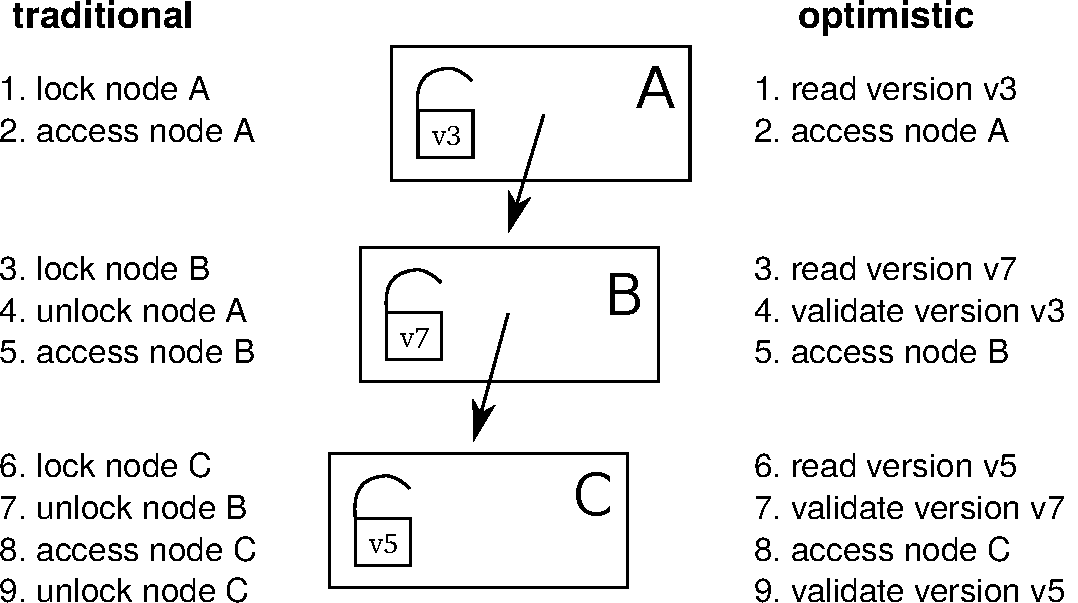
\includegraphics[width=0.65\linewidth]{olcall.pdf}
  \vspace{0.2cm}
  \caption{Comparison of a lookup operation in a 3-level tree using traditional lock coupling (left-hand side) vs.~optimistic lock coupling (right-hand side).}
  \label{fig:olc}
\end{figure}

The traditional and most common lock-based synchronization protocol for B-trees is lock coupling, which interleaves lock acquisitions while holding at most two locks at a time.
If, as we observed earlier, optimistic locks have similar semantics as traditional locks, it is natural to ask whether lock coupling can be combined with optimistic locks.
And indeed the answer is yes: One can almost mechanically translate traditional lock coupling code to optimistic lock coupling code.
This is illustrated in Figure~\ref{fig:olc}, which compares the traversal in a tree of height 3 using traditional and optimistic locks.
As the figure shows, the main difference is that locking is translated to reading the version and that unlocking becomes validation of the previously read version.
This simple change provides efficient lock-free tree traversal without the need to design a complex synchronization protocol.

It is important to emphasize the conceptual simplicity of OLC in comparison to data structures that use custom protocols like the Bw-tree~\cite{DBLP:conf/icde/LevandoskiLS13a}.
To implement lock-free access, the Bw-tree requires an indirection table, delta nodes, complex splitting and merging logic, retry logic, etc.
OLC, on the other hand, can directly be applied to B-trees mostly by adding the appropriate optimistic locking code and without modifying the node layout itself.
Therefore, OpenBw-Tree, an open source implementation of the Bw-tree, requires an order of magnitude more code than a B-tree based on OLC\footnote{Both implementations are available on GitHub: \url{https://github.com/wangziqi2016/index-microbench}}.
Given how difficult it is to develop, validate, and debug lock-free code, simplicity is obviously a major advantage.

\subsection{Correctness Aspects}

\begin{figure}
  % \centering
  %[basicstyle=\normalsize\ttfamily,showstringspaces=false,columns=fullflexible,breaklines=false,breakatwhitespace=true,numbers=none,numberstyle=\small,style=C,keepspaces=true]
\begin{lstlisting}[basicstyle=\ttfamily,language=C++,numbers=left,numberstyle=\small]
std::atomic<BTreeNode*> root;

// search for key in B+tree, returns payload in resultOut
bool lookup(Key key, Value& resultOut) {
   BTreeNode* node = root.load();
   uint64_t nodeVersion = node->readLockOrRestart();
   if (node != root.load()) // make sure the root is still the root
      restart();

   BTreeInner<Key>* parent = nullptr;
   uint64_t parentVersion = 0;

   while (node->isInner()) {
      auto inner = (BTreeInner*)node;

      // unlock parent and make current node the parent
      if (parent)
         parent->readUnlockOrRestart(parentVersion);
      parent = inner;
      parentVersion = nodeVersion;

      // search for next node
      node = inner->findChild(key);
      // validate 'inner' to ensure that 'node' pointer is valid
      inner->checkOrRestart(nodeVersion);
      // now it safe to dereference 'node' pointer (read its version)
      nodeVersion = node->readLockOrRestart();
   }

   // search in leaf and retrieve payload
   auto leaf = (BTreeLeaf*)node;
   bool success = leaf->findValue(key, resultOut);

   // unlock everything
   if (parent)
      parent->readUnlockOrRestart(parentVersion);
   node->readUnlockOrRestart(nodeVersion);

   return success;
}
\end{lstlisting}
  \vspace{0.2cm}
  \caption{B-tree lookup code using OLC. For simplicity, the restart logic is not shown.}
  \label{fig:lookup}
\end{figure}

So far, we have introduced the high-level ideas behind OLC and have stressed its similarity to traditional lock coupling.
Let us now discuss some cases where the close similarity between lock coupling and OLC breaks down.
To make this more concrete, we show the B-tree lookup code in Figure~\ref{fig:lookup}.
In the code, \texttt{readLockOrRestart} reads the lock version and \texttt{readUnlockOrRestart} validates that the read was correct.

One issue with OLC is that any pointer speculatively read from a node may point to invalid memory (if that node is modified concurrently).
Dereferencing such a pointer (e.g., to read its optimistic lock), may cause a segmentation fault or undefined behavior.
In the code shown in Figure~\ref{fig:lookup}, this problem is prevented by the extra check in line 25, which ensures that the read from the node containing the pointer was correct.
Without this additional validation, the code would in line 27 dereference the pointer speculatively read in line 23.
Note that the implementation of \texttt{checkOrRestart} is actually identical to \texttt{readUnlockOrRestart}.
We chose to give it a different name to highlight the fact that this extra check would not be necessary with read/write locks.

Another potential issue with optimistic locks is code that does not terminate.
Code that speculatively accesses a node, like an intra-node binary search, should be written in a way such that it always terminates---even in the presence of concurrent writes.
Otherwise, the validation code that detects the concurrent write will never run.
The binary search of a B-tree, for example, needs to be written in such a way that each comparison makes progress.
For some data structures that do not require loops in the traversal code (like ART) termination is trivially true.

\subsection{Implementation Details}

% implementation, efficiency
To implement an optimistic lock, one can combine the lock and the version counter into a single 64-bit\footnote{Even after subtracting one bit for the lock status, a back-of-the-envelope calculation can show that 63 bits are large enough to never overflow in practice.} word~\cite{artsync}.
A typical read operation will therefore merely consist of reading this version counter atomically.
In C++11 this can be implemented using the \texttt{std::atomic} type.

On x86, atomic reads are cheap because of x86's strong memory order guarantees.
No memory fences are required for sequentially-consistent loads, which are translated (by both GCC and clang) into standard \texttt{MOV} instructions.
Hence, the only effect of \texttt{std::atomic} for loads is preventing instruction re-ordering.
This makes version access and validation cheap.
Acquiring and releasing an optimistic lock in exclusive mode has comparable cost to a traditional lock:
A fairly expensive sequentially-consistent store is needed for acquiring a lock, while a standard \texttt{MOV} suffices for releasing it.
A simple sinlock-based implementation of optimistic locks can be found in the appendix of an earlier paper~\cite{artsync}.

OLC code must be able to handle restarts since validation or lock upgrade can fail due to concurrent writers.
Restarts can easily be implemented by wrapping the data structure operation in a loop (for simplicity not shown in Figure~\ref{fig:lookup}).
Such a loop also enables limiting the number of optimistic retry operations and falling back to pessimistic locking in cases of very heavy contention.
The ability to fall back to traditional locking is a major advantage of OLC in terms of robustness over lock-free approaches, which do not have this option.

In addition to the optimistic shared mode and the exclusive mode, optimistic locks also support a ``shared pessimistic'' mode, which physically acquires the lock in shared mode (allowing multiple concurrent readers but no writers).
This mode is useful for table (or range) scans that touch many tuples on a leaf page (which would otherwise easily abort).
Finally, let us mention that large range scans and table scans, should be broken up into several per-node traversals as is done in the LeanStore~\cite{leanstore} system.

Like all lock-free data structures, but unlike traditional locking and Hardware Transactional Memory~\cite{DBLP:conf/hpca/KarnagelDRLLSL14,DBLP:journals/pvldb/MakreshanskiLS15,htmtkde}, OLC requires care when deleting (and reusing) nodes.
The reason is that a deleting thread can never be sure that a node can be reclaimed because other threads might still be optimistically reading from that node.
Therefore, standard solutions like epoch-based reclamation~\cite{DBLP:conf/sosp/TuZKLM13}, hazard pointers~\cite{DBLP:journals/tpds/Michael04}, or optimized hazard pointers~\cite{DBLP:conf/spaa/BalmauGHZ16} need to be used.
These memory reclamation techniques are, however, largely orthogonal to the synchronization protocol itself.

%-lock-free is not a strong guarantee

\newpage
\section{Evaluation}\label{sec:evaluation}

Let us now experimentally evaluate the overhead and scalability of OLC.
For the experiments, we use an in-memory B+tree implemented in C++11 using templates, which is configured to use nodes of 4096 bytes, random 8 byte keys, and 8 byte payloads.
Based on this B-tree, we compare the following synchronization approaches:
\begin{itemize}
\item an OLC implementation\footnote{An almost identical OLC implementation is available on github: \url{https://github.com/wangziqi2016/index-microbench/tree/master/BTreeOLC}}
\item a variant based on traditional lock coupling and read/write locks
\item the unsynchronized B-tree, which obviously is only correct for read-only workloads but allows measuring the overhead of synchronization
\end{itemize}
Note that earlier work has compared the OLC implementation with a Bw-tree implementation~\cite{buzzword} and other state-of-the-art in-memory index structures.

We use a Haswell EP system with an Intel Xeon E5-2687W v3 CPU, which has 10 cores (20 ``Hyper-Threads'') and 25~MB of L3 cache.
The system is running Ubuntu 18.10 and we use GCC 8.2.0 to compile our code.
The CPU counters are obtained using the Linux perf API\footnote{We use the following convenience wrapper: \url{https://github.com/viktorleis/perfevent}}.

\begin{table}
  \caption{Performance and CPU counters for lookup and insert operations in a B-tree with 100M keys. We perform 100M operations and normalize the CPU counters by that number.}
  \label{tab:overhead}
  \centering
  \begin{tabular}{lrrrrrrr}\toprule
                    &         &        &        & instruc-  & L1     & L3     & branch \\
                    & threads & M op/s & cycles & tions & misses & misses & misses \\\midrule
lookup (no sync.)   & 1       & 1.72   & 2028   & 283     & 39.1   & 14.9   & 16.1   \\
lookup (OLC)        & 1       & 1.65   & 2107   & 370     & 43.9   & 15.1   & 16.7   \\
lookup (lock coup.) & 1       & 1.72   & 2078   & 365     & 42.3   & 16.9   & 15.7   \\\midrule
insert (no sync.)   & 1       & 1.51   & 2286   & 530     & 59.8   & 31.1   & 17.3   \\
insert (OLC)        & 1       & 1.50   & 2303   & 629     & 61.2   & 31.1   & 16.5   \\
insert (lock coup.) & 1       & 1.41   & 2473   & 644     & 61.0   & 31.0   & 17.2   \\\midrule
lookup (no sync.)   & 10      & 15.48  & 2058   & 283     & 38.6   & 15.5   & 16.0   \\
lookup (OLC)        & 10      & 14.60  & 2187   & 370     & 43.8   & 15.8   & 16.8   \\
lookup (lock coup.) & 10      & 5.71   & 5591   & 379     & 54.2   & 17.0   & 14.8   \\\midrule
insert (no sync.)   & 10      & -      & -      & -       & -      & -      & -      \\
insert (OLC)        & 10      & 10.46  & 2940   & 656     & 62.0   & 32.5   & 16.8   \\
insert (lock coup.) & 10      & 7.55   & 4161   & 667     & 75.0   & 28.6   & 16.2   \\
    \bottomrule
\end{tabular}
\end{table}

Table~\ref{tab:overhead} compares the performance and CPU counters for lookup and insert operations in a B-tree with 100M keys.
With {\em single-threaded} execution, we observe that all three approaches have very similar performance.
Adding traditional or optimistic locks to unsynchronized B-tree code results in up to 30\% of additional instructions without affecting single-threaded performance much.

\begin{figure}
  \centering
  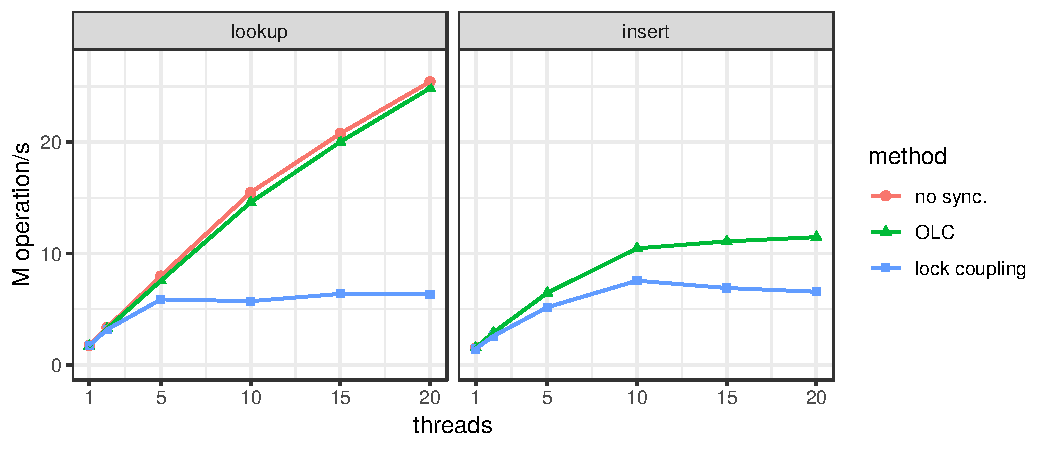
\includegraphics[width=\linewidth]{scale.pdf}
  \vspace{0.2cm}
  \caption{Scalability on 10-core system for B-tree operations (100M values).}
  \label{fig:scale}
\end{figure}

As Figure~\ref{fig:scale} shows, the results change dramatically once we use multiple threads.
For lookup, the scalability of OLC is near-linear up to 20 threads, even though the system has only 10 ``real cores''.
The OLC scalability for insert is also respectable (though not quite as linear because multi-threaded insertion approaches the memory bandwidth of our processor).
The figure also shows that the results of traditional lock coupling with read/write locks are significantly worse than OLC.
With 20 threads, lookup with OLC is 3.9$\times$ faster than traditional lock coupling.

\section{Summary}\label{sec:conc}

Optimistic Lock Coupling (OLC) is an effective synchronization method that combines the simplicity of traditional lock coupling with the superior scalability of lock-free approaches.
OLC is widely applicable and has already been successfully used to synchronize several data structures, including B-trees, binary search trees, and different trie variants.
These features make it highly attractive for modern database systems as well as performance-critical systems software in general.

\begin{thebibliography}{10}

\bibitem{DBLP:conf/spaa/BalmauGHZ16}
O.~Balmau, R.~Guerraoui, M.~Herlihy, and I.~Zablotchi.
\newblock Fast and robust memory reclamation for concurrent data structures.
\newblock In {\em SPAA}, 2016.

\bibitem{DBLP:journals/acta/BayerS77}
R.~Bayer and M.~Schkolnick.
\newblock Concurrency of operations on {B}-trees.
\newblock {\em Acta Informatica}, 9, 1977.

\bibitem{hot}
R.~Binna, E.~Zangerle, M.~Pichl, G.~Specht, and V.~Leis.
\newblock {HOT}: A height optimized trie index for main-memory database
  systems.
\newblock In {\em SIGMOD}, 2018.

\bibitem{DBLP:conf/ppopp/BronsonCCO10}
N.~G. Bronson, J.~Casper, H.~Chafi, and K.~Olukotun.
\newblock A practical concurrent binary search tree.
\newblock In {\em PPOPP}, 2010.

\bibitem{DBLP:conf/vldb/ChaHKK01}
S.~K. Cha, S.~Hwang, K.~Kim, and K.~Kwon.
\newblock Cache-conscious concurrency control of main-memory indexes on
  shared-memory multiprocessor systems.
\newblock In {\em VLDB}, 2001.

\bibitem{intel}
I.~Cutress.
\newblock {Intel} goes for 48-cores: {Cascade-AP} with multi-chip package
  coming soon.
\newblock
  \url{https://www.anandtech.com/show/13535/intel-goes-for-48cores-cascade-ap},
  2018 (accessed January, 2019).

\bibitem{DBLP:conf/cidr/FaleiroA17}
J.~M. Faleiro and D.~J. Abadi.
\newblock Latch-free synchronization in database systems: Silver bullet or
  fool's gold?
\newblock In {\em CIDR}, 2017.

\bibitem{DBLP:journals/ftdb/Graefe11}
G.~Graefe.
\newblock Modern {B}-tree techniques.
\newblock {\em Foundations and Trends in Databases}, 3(4), 2011.

\bibitem{DBLP:conf/hpca/KarnagelDRLLSL14}
T.~Karnagel, R.~Dementiev, R.~Rajwar, K.~Lai, T.~Legler, B.~Schlegel, and
  W.~Lehner.
\newblock Improving in-memory database index performance with
  {Intel}\({}^{\mbox{{\textregistered}}}\) transactional synchronization
  extensions.
\newblock In {\em HPCA}, 2014.

\bibitem{DBLP:journals/tods/LehmanY81}
P.~L. Lehman and S.~B. Yao.
\newblock Efficient locking for concurrent operations on {B}-trees.
\newblock {\em {ACM} Trans. Database Syst.}, 6(4), 1981.

\bibitem{leanstore}
V.~Leis, M.~Haubenschild, A.~Kemper, and T.~Neumann.
\newblock Leanstore: In-memory data management beyond main memory.
\newblock In {\em ICDE}, 2018.

\bibitem{art}
V.~Leis, A.~Kemper, and T.~Neumann.
\newblock The adaptive radix tree: {ARTful} indexing for main-memory databases.
\newblock In {\em ICDE}, 2013.

\bibitem{htmtkde}
V.~Leis, A.~Kemper, and T.~Neumann.
\newblock Scaling {HTM}-supported database transactions to many cores.
\newblock {\em {IEEE} Trans. Knowl. Data Eng.}, 28(2), 2016.

\bibitem{artsync}
V.~Leis, F.~Scheibner, A.~Kemper, and T.~Neumann.
\newblock The {ART} of practical synchronization.
\newblock In {\em DaMoN}, 2016.

\bibitem{DBLP:conf/icde/LevandoskiLS13a}
J.~J. Levandoski, D.~B. Lomet, and S.~Sengupta.
\newblock The {Bw}-tree: A {B}-tree for new hardware platforms.
\newblock In {\em ICDE}, 2013.

\bibitem{DBLP:journals/pvldb/MakreshanskiLS15}
D.~Makreshanski, J.~J. Levandoski, and R.~Stutsman.
\newblock To lock, swap, or elide: On the interplay of hardware transactional
  memory and lock-free indexing.
\newblock {\em {PVLDB}}, 8(11), 2015.

\bibitem{DBLP:dblp_conf/eurosys/MaoKM12}
Y.~Mao, E.~Kohler, and R.~T. Morris.
\newblock Cache craftiness for fast multicore key-value storage.
\newblock In {\em EuroSys}, 2012.

\bibitem{DBLP:journals/tpds/Michael04}
M.~M. Michael.
\newblock Hazard pointers: Safe memory reclamation for lock-free objects.
\newblock {\em {IEEE} Trans. Parallel Distrib. Syst.}, 15(6), 2004.

\bibitem{DBLP:journals/jacm/ShalevS06}
O.~Shalev and N.~Shavit.
\newblock Split-ordered lists: Lock-free extensible hash tables.
\newblock {\em J. {ACM}}, 53(3), 2006.

\bibitem{amd}
A.~Shilov.
\newblock {AMD} previews {EPYC} ‘{Rome}’ processor: Up to 64 {Zen} 2 cores.
\newblock
  \url{https://www.anandtech.com/show/13561/amd-previews-epyc-rome-processor-up-to-64-zen-2-cores},
  2018 (accessed January, 2019).

\bibitem{DBLP:conf/sosp/TuZKLM13}
S.~Tu, W.~Zheng, E.~Kohler, B.~Liskov, and S.~Madden.
\newblock Speedy transactions in multicore in-memory databases.
\newblock In {\em SOSP}, 2013.

\bibitem{buzzword}
Z.~Wang, A.~Pavlo, H.~Lim, V.~Leis, H.~Zhang, M.~Kaminsky, and D.~Andersen.
\newblock Building a {Bw}-tree takes more than just buzz words.
\newblock In {\em SIGMOD}, 2018.

\end{thebibliography}


%\bibliographystyle{abbrv}
%\bibliography{main}

\end{document}

\end{article}


\begin{article}
{FedCLIP: Fast Generalization and Personalization for CLIP in Federated Learning}
{Wang Lu, Xixu Hu, Jindong Wang, and Xing Xie}
\pdfminorversion=5
\documentclass[11pt]{article}
\usepackage{deauthor,times,graphicx,caption,microtype}
\usepackage{hyperref}
\usepackage{listings}
\usepackage{booktabs}

\begin{document}

\title{Optimistic Lock Coupling: A Scalable and Efficient General-Purpose Synchronization Method}

\author{Viktor Leis, Michael Haubenschild\raisebox{0.9ex}{$\ast$}, Thomas Neumann\\ Technische Universit{\"a}t M{\"u}nchen \hspace{0.7cm} Tableau Software\raisebox{0.9ex}{$\ast$} \\ {\{leis,neumann\}{@}in.tum.de} \hspace{0.7cm} {mhaubenschild{@}tableau.com\raisebox{0.9ex}{$\ast$}}}

\maketitle

\begin{abstract}
As the number of cores on commodity processors continues to increase, scalability becomes more and more crucial for overall performance.
Scalable and efficient concurrent data structures are particularly important, as these are often the building blocks of parallel algorithms.
Unfortunately, traditional synchronization techniques based on fine-grained locking have been shown to be unscalable on modern multi-core CPUs.
Lock-free data structures, on the other hand, are extremely difficult to design and often incur significant overhead.

In this work, we make the case for Optimistic Lock Coupling as a practical alternative to both traditional locking and the lock-free approach.
We show that Optimistic Lock Coupling is highly scalable and almost as simple to implement as traditional lock coupling.
Another important advantage is that it is easily applicable to most tree-like data structures.
We therefore argue that Optimistic Lock Coupling, rather than a complex and error-prone custom synchronization protocol, should be the default choice for performance-critical data structures.
\end{abstract}

\section{Introduction}

% more and more cores
Today, Intel's commodity server processors have up to 28 cores and its upcoming microarchitecture will have up to 48 cores per socket~\cite{intel}.
Similarly, AMD currently stands at 32 cores and this number is expected to double in the next generation~\cite{amd}.
Since both platforms support simultaneous multithreading (also known as hyperthreading), affordable commodity servers (with up to two sockets) will soon routinely have between 100 and 200 hardware threads.

% data structure scalability is important
With such a high degree of hardware parallelism, efficient data processing crucially depends on how well concurrent data structures scale.
Internally, database systems use a plethora of data structures like table heaps, internal work queues, and, most importantly, index structures.
Any of these can easily become a scalability (and therefore overall performance) bottleneck on many-core CPUs.

% traditional synchronization: fine-grained locks, slow, cache invalidation
Traditionally, database systems synchronize internal data structures using fine-grained reader/writer locks\footnote{In this work, we focus on data structure synchronization rather than high-level transaction semantics and therefore use the term {\em lock} for what would typically be called {\em latch} in the database literature. We thus follow common computer science (rather than database) terminology.}.
Unfortunately, while fine-grained locking makes lock contention unlikely, it still results in bad scalability because lock acquisition and release require writing to shared memory.
Due to the way cache coherency is implemented on modern multi-core CPUs, these writes cause additional cache misses\footnote{The cache coherency protocol ensures that all copies of a cache line on other cores are invalidated before the write can proceed.} and the cache line containing the lock's internal data becomes a point of physical contention.
As a result, any frequently-accessed lock (e.g., the lock of the root node of a B-tree) severely limits scalability.

% lock-free bw-tree: no more latches, but indirections, extremely complex
Lock-free data structures like the Bw-tree~\cite{DBLP:conf/icde/LevandoskiLS13a} (a lock-free B-tree variant) or the Split-Ordered List~\cite{DBLP:journals/jacm/ShalevS06} (a lock-free hash table) do not acquire any locks and therefore generally scale much better than locking-based approaches (in particular for read-mostly workloads).
However, lock-free synchronization has other downsides:
First, it is very difficult and results in extremely complex and error-prone code (when compared to locking).
Second, because the functionality of atomic primitives provided by the hardware (e.g., atomically compare-and-swap 8 bytes) is limited, complex operations require additional indirections within the data structure.
For example, the Bw-tree requires an indirection table and the Split-Ordered List requires ``dummy nodes'', resulting in overhead due to additional cache misses.

% OLC for the win
In this paper we make the case for {\em Optimistic Lock Coupling (OLC)}, a synchronization method that combines some of the best properties of lock-based and lock-free synchronization.
OLC utilizes a special lock type that can be used in two modes:
The first mode is similar to a traditional mutex and excludes other threads by physically acquiring the underlying lock.
In the second mode, reads can proceed optimistically by validating a version counter that is embedded in the lock (similar to optimistic concurrency control).
The first mode is typically used by writers and the second mode by readers.
Besides this special lock type, OLC is based on the observation that optimistic lock validations can be interleaved/coupled---similar to the pair-wise interleaved lock acquisition of traditional lock coupling.
Hence, the name Optimistic Lock Coupling.

OLC has a number of desirable features:
\begin{itemize}
\item By reducing the number of writes to shared memory locations and thereby avoiding cache invalidations, it {\bf scales well} for most workloads.
\item In comparison to unsynchronized code, it requires few additional CPU instructions making it {\bf efficient}.
\item OLC is {\bf widely applicable} to different data structures. It has already been successfully used for synchronizing binary search trees~\cite{DBLP:conf/ppopp/BronsonCCO10}, tries~\cite{artsync}, trie/B-tree hybrids~\cite{DBLP:dblp_conf/eurosys/MaoKM12}, and B-trees~\cite{buzzword}.
\item In comparison to the lock-free paradigm, it is also {\bf easy to use} and requires few modifications to existing, single-threaded data structures.
\end{itemize}
Despite these positive features and its simplicity, OLC is not yet widely known.
The goal of this paper is therefore to popularize this simple idea and to make a case for it.
We argue that OLC deserves to be widely known.
It is a good default synchronization paradigm---more complex, data structure-specific protocols are seldom beneficial.

The rest of the paper is organized as follows.
Section~\ref{sec:related} discusses related work, tracing the history of OLC and its underlying ideas in the literature.
The core of the paper is Section~\ref{sec:olc}, which describes the ideas behind OLC and how it can be used to synchronize complex data structures.
In Section~\ref{sec:evaluation} we experimentally show that OLC has low overhead and scales well when used to synchronize an in-memory B-tree.
We summarize the paper in Section~\ref{sec:conc}.

\newpage
\section{Related Work}\label{sec:related}

Lock coupling has been proposed as a method for allowing concurrent operations on B-trees in 1977~\cite{DBLP:journals/acta/BayerS77}.
This traditional and still widely-used method, described in detail in Graefe's B-tree survey~\cite{DBLP:journals/ftdb/Graefe11}, is also called ``latch coupling'', ``hand-over-hand locking'', and ``crabbing''.
Because at most two locks are held at-a-time during tree traversal, this technique seemingly allows for a high degree of parallelism---in particular if read/write locks are used to enable inner nodes to be locked in shared mode.
However, as we show in Section~\ref{sec:evaluation}, on modern hardware lock acquisition (even in shared mode) results in suboptimal scalability.

An early alternative from 1981 is a B-tree variant called B-link tree~\cite{DBLP:journals/tods/LehmanY81}, which only holds a single lock at a time.
It is based on the observation that between the release of the parent lock and the acquisition of the child lock, the only ``dangerous'' thing that could have happened is the split of a child node (assuming one does not implement merge operations).
Thus, when a split happens, the key being searched might end up on a neighboring node to the right of the current child node.
A B-link tree traversal therefore detects this condition and, if needed, transparently proceeds to the neighboring node.
Releasing the parent lock early is highly beneficial when the child node needs to be fetched from disk.
For in-memory workloads, however, the B-link tree has the same scalability issues as lock coupling (it acquires just as many locks).

The next major advance, Optimistic Latch-Free Index Traversal (OLFIT)~\cite{DBLP:conf/vldb/ChaHKK01}, was proposed in 2001.
OLFIT introduced the idea of a combined lock/update counter, which we call {\em optimistic lock}. % , for lack of a better name,
Based on these per-node optimistic locks and the synchronization protocol of the B-link tree, OLFIT finally achieves good scalability on parallel processors.
The OLFIT protocol is fairly complex, as it requires both the non-trivial B-link protocol and optimistic locks.
Furthermore, like the B-link tree protocol, it does not support merging nodes, and is specific to B-trees (cannot easily be applied to other data structures).

In the following two decades, the growth of main-memory capacity led to much research into other data structures besides the venerable B-tree.
Particularly relevant for our discussion is Bronson et al.'s~\cite{DBLP:conf/ppopp/BronsonCCO10} concurrent binary search tree, which is based on optimistic version validation and has a sophisticated, data structure-specific synchronization protocol.
To the best of our knowledge, this 2010 paper is the first that, as part of its protocol, interleaves version validation across nodes---rather than validating each node separately like OLFIT.
In that paper, this idea is called ``hand-over-hand, optimistic validation'', while we prefer the term Optimistic Lock Coupling to highlight the close resemblance to traditional lock coupling.
Similarly, Mao et al.'s~\cite{DBLP:dblp_conf/eurosys/MaoKM12} Masstree (a concurrent hybrid trie/B-tree) is also based on the same ideas, but again uses them as part of a more complex protocol.

The Adaptive Radix Tree (ART)~\cite{art} is another recent in-memory data structure, which we proposed in 2013.
In contrast to the two data structures just mentioned, it was originally designed with single-threaded performance in mind without supporting concurrency.
To add support for concurrency, we initially started designing a custom protocol called Read-Optimized Write Exclusion (ROWEX)~\cite{artsync}, which turned out to be non-trivial and requires modifications of the underlying data structure\footnote{Note that ROWEX is already easier to apply to existing data structures than the lock-free approach. The difficulty depends on the data structure. Applying ROWEX is hard for B-trees with sorted keys and fairly easy for copy-on-write data structures like the Height Optimized Trie~\cite{hot}---with ART being somewhere in the middle.}.
However, fairly late in the project, we also realized, that OLC {\em alone} (rather than as part of a more complex protocol) is sufficient to synchronize ART.
No other changes to the data structure were necessary.
Both approaches were published and experimentally evaluated in a followup paper~\cite{artsync}, which shows that, despite its simplicity, OLC is efficient, scalable, and generally outperforms ROWEX.

Similar results were recently published regarding B-trees~\cite{buzzword}.
In this experimental study a simple OLC-based synchronization outperformed the Bw-tree~\cite{DBLP:conf/icde/LevandoskiLS13a}, a complex lock-free synchronization approach.
Another recent paper shows that for write-intensive workloads, locking often performs better than lock-free synchronization~\cite{DBLP:conf/cidr/FaleiroA17}.
These experiences indicate that OLC is a general-purpose synchronization paradigm and motivate the current paper.

%foster b-tree\cite{DBLP:journals/tods/GraefeKK12}
%Shasha theory~\cite{DBLP:journals/tods/ShashaG88}

\section{Optimistic Lock Coupling}\label{sec:olc}

% locks suck
The standard technique for inter-thread synchronization is mutual exclusion using fine-grained locks.
In a B-tree, for example, every node usually has its own associated lock, which is acquired before accessing that node.
The problem of locking on modern multi- and many-core processors is that lock acquisition and release require writing to the shared memory location that implements the lock.
This write causes exclusive ownership of the underlying cache line and invalidates copies of it on all other processor cores.
For hierarchical, tree-like data structures, the lock of the root node becomes a point of physical contention---even in read-only workloads and even when read/write locks are used.
Depending on the specific data structure, number of cores, cache coherency protocol implementation, cache topology, whether Non-Uniform Memory Access (NUMA) is used, locking can even result in multi-threaded performance that is worse than single-threaded execution.

% in b-trees this happens very much
The inherent pessimism of locking is particularly unfortunate for B-trees:
Despite the fact that logical modifications of the root node are very infrequent, every B-tree operation must lock the root node during tree traversal\footnote{To a lesser extent this obviously applies to all inner nodes, not just the root.}.
Even the vast majority of update operations (with the exception of splits and merges), only modify a single leaf node.
These observations indicate that a more optimistic approach, which does not require locking inner nodes, would be very beneficial for B-trees.

\subsection{Optimistic Locks}

% optimism to the rescue
As the name indicates, optimistic locks try to solve the scalability issues of traditional locks using an optimistic approach.
Instead of always physically acquiring locks, even for nodes that are unlikely to be modified simultaneously, after-the-fact validation is used to detect conflicts.
This is done by augmenting each lock with a version/update counter that is incremented on every modification.
Using this version counter, readers can optimistically proceed before validating that the version did not change to ensure that the read was safe.
If validation fails, the operation is restarted.

% details on opt locks
Using optimistic locks, a read-only node access (i.e., the majority of all operations in a B-tree) does not acquire the lock and does not increment the version counter.
Instead, it performs the following steps:
\begin{enumerate}
\item read lock version (restart if lock is not free)
\item access node
\item read the version again and validate that it has not changed in the meantime
\end{enumerate}
If the last step (the validation) fails, the operation has to be restarted.
Write operations, on the other hand, are more similar to traditional locking:
\begin{enumerate}
\item acquire lock (wait if necessary)
\item access/write to node
\item increment version and unlock node
\end{enumerate}
Writes can therefore protect a node from other writes.

% similar to locks
As we observed in an earlier paper~\cite{artsync}, because of similar semantics, optimistic locks can be hidden behind an API very similar to traditional read/write locks.
Both approaches have an exclusive lock mode, and acquiring a traditional lock in shared mode is analogous to optimistic version validation.
Furthermore, like with some implementations of traditional read/write locks, optimistic locks allow upgrading a shared lock to an exclusive lock.
Lock upgrades are, for example, used to avoid most B-tree update operations from having to lock inner nodes.
In our experience, the close resemblance of optimistic and traditional locks simplifies the reasoning about optimistic locks;
one can apply similar thinking as in traditional lock-based protocols.

\subsection{Lock Coupling with Optimistic Locks}

\begin{figure}
  \centering
  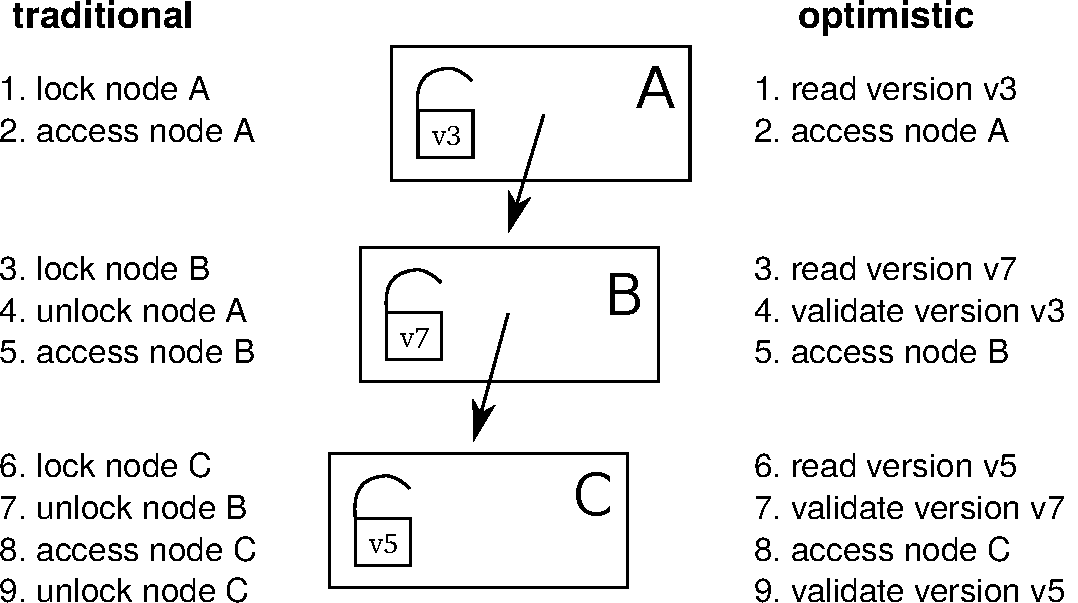
\includegraphics[width=0.65\linewidth]{olcall.pdf}
  \vspace{0.2cm}
  \caption{Comparison of a lookup operation in a 3-level tree using traditional lock coupling (left-hand side) vs.~optimistic lock coupling (right-hand side).}
  \label{fig:olc}
\end{figure}

The traditional and most common lock-based synchronization protocol for B-trees is lock coupling, which interleaves lock acquisitions while holding at most two locks at a time.
If, as we observed earlier, optimistic locks have similar semantics as traditional locks, it is natural to ask whether lock coupling can be combined with optimistic locks.
And indeed the answer is yes: One can almost mechanically translate traditional lock coupling code to optimistic lock coupling code.
This is illustrated in Figure~\ref{fig:olc}, which compares the traversal in a tree of height 3 using traditional and optimistic locks.
As the figure shows, the main difference is that locking is translated to reading the version and that unlocking becomes validation of the previously read version.
This simple change provides efficient lock-free tree traversal without the need to design a complex synchronization protocol.

It is important to emphasize the conceptual simplicity of OLC in comparison to data structures that use custom protocols like the Bw-tree~\cite{DBLP:conf/icde/LevandoskiLS13a}.
To implement lock-free access, the Bw-tree requires an indirection table, delta nodes, complex splitting and merging logic, retry logic, etc.
OLC, on the other hand, can directly be applied to B-trees mostly by adding the appropriate optimistic locking code and without modifying the node layout itself.
Therefore, OpenBw-Tree, an open source implementation of the Bw-tree, requires an order of magnitude more code than a B-tree based on OLC\footnote{Both implementations are available on GitHub: \url{https://github.com/wangziqi2016/index-microbench}}.
Given how difficult it is to develop, validate, and debug lock-free code, simplicity is obviously a major advantage.

\subsection{Correctness Aspects}

\begin{figure}
  % \centering
  %[basicstyle=\normalsize\ttfamily,showstringspaces=false,columns=fullflexible,breaklines=false,breakatwhitespace=true,numbers=none,numberstyle=\small,style=C,keepspaces=true]
\begin{lstlisting}[basicstyle=\ttfamily,language=C++,numbers=left,numberstyle=\small]
std::atomic<BTreeNode*> root;

// search for key in B+tree, returns payload in resultOut
bool lookup(Key key, Value& resultOut) {
   BTreeNode* node = root.load();
   uint64_t nodeVersion = node->readLockOrRestart();
   if (node != root.load()) // make sure the root is still the root
      restart();

   BTreeInner<Key>* parent = nullptr;
   uint64_t parentVersion = 0;

   while (node->isInner()) {
      auto inner = (BTreeInner*)node;

      // unlock parent and make current node the parent
      if (parent)
         parent->readUnlockOrRestart(parentVersion);
      parent = inner;
      parentVersion = nodeVersion;

      // search for next node
      node = inner->findChild(key);
      // validate 'inner' to ensure that 'node' pointer is valid
      inner->checkOrRestart(nodeVersion);
      // now it safe to dereference 'node' pointer (read its version)
      nodeVersion = node->readLockOrRestart();
   }

   // search in leaf and retrieve payload
   auto leaf = (BTreeLeaf*)node;
   bool success = leaf->findValue(key, resultOut);

   // unlock everything
   if (parent)
      parent->readUnlockOrRestart(parentVersion);
   node->readUnlockOrRestart(nodeVersion);

   return success;
}
\end{lstlisting}
  \vspace{0.2cm}
  \caption{B-tree lookup code using OLC. For simplicity, the restart logic is not shown.}
  \label{fig:lookup}
\end{figure}

So far, we have introduced the high-level ideas behind OLC and have stressed its similarity to traditional lock coupling.
Let us now discuss some cases where the close similarity between lock coupling and OLC breaks down.
To make this more concrete, we show the B-tree lookup code in Figure~\ref{fig:lookup}.
In the code, \texttt{readLockOrRestart} reads the lock version and \texttt{readUnlockOrRestart} validates that the read was correct.

One issue with OLC is that any pointer speculatively read from a node may point to invalid memory (if that node is modified concurrently).
Dereferencing such a pointer (e.g., to read its optimistic lock), may cause a segmentation fault or undefined behavior.
In the code shown in Figure~\ref{fig:lookup}, this problem is prevented by the extra check in line 25, which ensures that the read from the node containing the pointer was correct.
Without this additional validation, the code would in line 27 dereference the pointer speculatively read in line 23.
Note that the implementation of \texttt{checkOrRestart} is actually identical to \texttt{readUnlockOrRestart}.
We chose to give it a different name to highlight the fact that this extra check would not be necessary with read/write locks.

Another potential issue with optimistic locks is code that does not terminate.
Code that speculatively accesses a node, like an intra-node binary search, should be written in a way such that it always terminates---even in the presence of concurrent writes.
Otherwise, the validation code that detects the concurrent write will never run.
The binary search of a B-tree, for example, needs to be written in such a way that each comparison makes progress.
For some data structures that do not require loops in the traversal code (like ART) termination is trivially true.

\subsection{Implementation Details}

% implementation, efficiency
To implement an optimistic lock, one can combine the lock and the version counter into a single 64-bit\footnote{Even after subtracting one bit for the lock status, a back-of-the-envelope calculation can show that 63 bits are large enough to never overflow in practice.} word~\cite{artsync}.
A typical read operation will therefore merely consist of reading this version counter atomically.
In C++11 this can be implemented using the \texttt{std::atomic} type.

On x86, atomic reads are cheap because of x86's strong memory order guarantees.
No memory fences are required for sequentially-consistent loads, which are translated (by both GCC and clang) into standard \texttt{MOV} instructions.
Hence, the only effect of \texttt{std::atomic} for loads is preventing instruction re-ordering.
This makes version access and validation cheap.
Acquiring and releasing an optimistic lock in exclusive mode has comparable cost to a traditional lock:
A fairly expensive sequentially-consistent store is needed for acquiring a lock, while a standard \texttt{MOV} suffices for releasing it.
A simple sinlock-based implementation of optimistic locks can be found in the appendix of an earlier paper~\cite{artsync}.

OLC code must be able to handle restarts since validation or lock upgrade can fail due to concurrent writers.
Restarts can easily be implemented by wrapping the data structure operation in a loop (for simplicity not shown in Figure~\ref{fig:lookup}).
Such a loop also enables limiting the number of optimistic retry operations and falling back to pessimistic locking in cases of very heavy contention.
The ability to fall back to traditional locking is a major advantage of OLC in terms of robustness over lock-free approaches, which do not have this option.

In addition to the optimistic shared mode and the exclusive mode, optimistic locks also support a ``shared pessimistic'' mode, which physically acquires the lock in shared mode (allowing multiple concurrent readers but no writers).
This mode is useful for table (or range) scans that touch many tuples on a leaf page (which would otherwise easily abort).
Finally, let us mention that large range scans and table scans, should be broken up into several per-node traversals as is done in the LeanStore~\cite{leanstore} system.

Like all lock-free data structures, but unlike traditional locking and Hardware Transactional Memory~\cite{DBLP:conf/hpca/KarnagelDRLLSL14,DBLP:journals/pvldb/MakreshanskiLS15,htmtkde}, OLC requires care when deleting (and reusing) nodes.
The reason is that a deleting thread can never be sure that a node can be reclaimed because other threads might still be optimistically reading from that node.
Therefore, standard solutions like epoch-based reclamation~\cite{DBLP:conf/sosp/TuZKLM13}, hazard pointers~\cite{DBLP:journals/tpds/Michael04}, or optimized hazard pointers~\cite{DBLP:conf/spaa/BalmauGHZ16} need to be used.
These memory reclamation techniques are, however, largely orthogonal to the synchronization protocol itself.

%-lock-free is not a strong guarantee

\newpage
\section{Evaluation}\label{sec:evaluation}

Let us now experimentally evaluate the overhead and scalability of OLC.
For the experiments, we use an in-memory B+tree implemented in C++11 using templates, which is configured to use nodes of 4096 bytes, random 8 byte keys, and 8 byte payloads.
Based on this B-tree, we compare the following synchronization approaches:
\begin{itemize}
\item an OLC implementation\footnote{An almost identical OLC implementation is available on github: \url{https://github.com/wangziqi2016/index-microbench/tree/master/BTreeOLC}}
\item a variant based on traditional lock coupling and read/write locks
\item the unsynchronized B-tree, which obviously is only correct for read-only workloads but allows measuring the overhead of synchronization
\end{itemize}
Note that earlier work has compared the OLC implementation with a Bw-tree implementation~\cite{buzzword} and other state-of-the-art in-memory index structures.

We use a Haswell EP system with an Intel Xeon E5-2687W v3 CPU, which has 10 cores (20 ``Hyper-Threads'') and 25~MB of L3 cache.
The system is running Ubuntu 18.10 and we use GCC 8.2.0 to compile our code.
The CPU counters are obtained using the Linux perf API\footnote{We use the following convenience wrapper: \url{https://github.com/viktorleis/perfevent}}.

\begin{table}
  \caption{Performance and CPU counters for lookup and insert operations in a B-tree with 100M keys. We perform 100M operations and normalize the CPU counters by that number.}
  \label{tab:overhead}
  \centering
  \begin{tabular}{lrrrrrrr}\toprule
                    &         &        &        & instruc-  & L1     & L3     & branch \\
                    & threads & M op/s & cycles & tions & misses & misses & misses \\\midrule
lookup (no sync.)   & 1       & 1.72   & 2028   & 283     & 39.1   & 14.9   & 16.1   \\
lookup (OLC)        & 1       & 1.65   & 2107   & 370     & 43.9   & 15.1   & 16.7   \\
lookup (lock coup.) & 1       & 1.72   & 2078   & 365     & 42.3   & 16.9   & 15.7   \\\midrule
insert (no sync.)   & 1       & 1.51   & 2286   & 530     & 59.8   & 31.1   & 17.3   \\
insert (OLC)        & 1       & 1.50   & 2303   & 629     & 61.2   & 31.1   & 16.5   \\
insert (lock coup.) & 1       & 1.41   & 2473   & 644     & 61.0   & 31.0   & 17.2   \\\midrule
lookup (no sync.)   & 10      & 15.48  & 2058   & 283     & 38.6   & 15.5   & 16.0   \\
lookup (OLC)        & 10      & 14.60  & 2187   & 370     & 43.8   & 15.8   & 16.8   \\
lookup (lock coup.) & 10      & 5.71   & 5591   & 379     & 54.2   & 17.0   & 14.8   \\\midrule
insert (no sync.)   & 10      & -      & -      & -       & -      & -      & -      \\
insert (OLC)        & 10      & 10.46  & 2940   & 656     & 62.0   & 32.5   & 16.8   \\
insert (lock coup.) & 10      & 7.55   & 4161   & 667     & 75.0   & 28.6   & 16.2   \\
    \bottomrule
\end{tabular}
\end{table}

Table~\ref{tab:overhead} compares the performance and CPU counters for lookup and insert operations in a B-tree with 100M keys.
With {\em single-threaded} execution, we observe that all three approaches have very similar performance.
Adding traditional or optimistic locks to unsynchronized B-tree code results in up to 30\% of additional instructions without affecting single-threaded performance much.

\begin{figure}
  \centering
  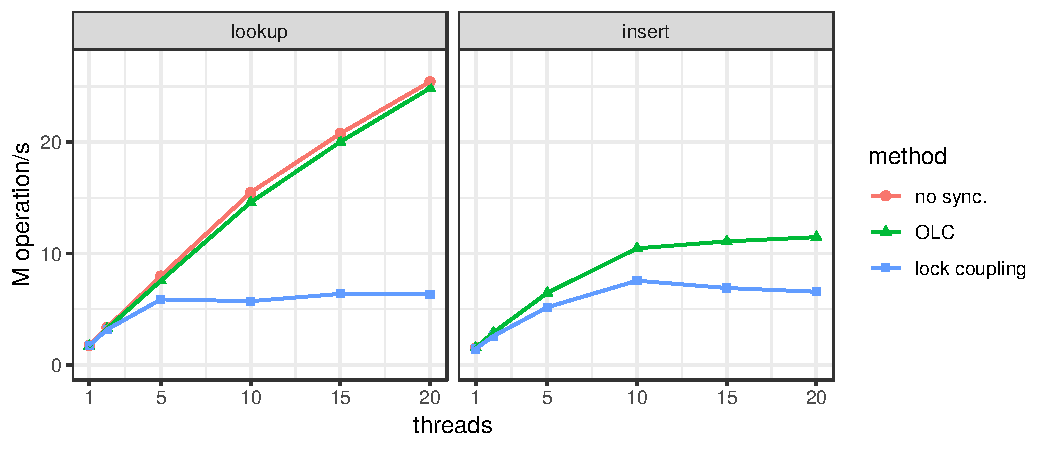
\includegraphics[width=\linewidth]{scale.pdf}
  \vspace{0.2cm}
  \caption{Scalability on 10-core system for B-tree operations (100M values).}
  \label{fig:scale}
\end{figure}

As Figure~\ref{fig:scale} shows, the results change dramatically once we use multiple threads.
For lookup, the scalability of OLC is near-linear up to 20 threads, even though the system has only 10 ``real cores''.
The OLC scalability for insert is also respectable (though not quite as linear because multi-threaded insertion approaches the memory bandwidth of our processor).
The figure also shows that the results of traditional lock coupling with read/write locks are significantly worse than OLC.
With 20 threads, lookup with OLC is 3.9$\times$ faster than traditional lock coupling.

\section{Summary}\label{sec:conc}

Optimistic Lock Coupling (OLC) is an effective synchronization method that combines the simplicity of traditional lock coupling with the superior scalability of lock-free approaches.
OLC is widely applicable and has already been successfully used to synchronize several data structures, including B-trees, binary search trees, and different trie variants.
These features make it highly attractive for modern database systems as well as performance-critical systems software in general.

\begin{thebibliography}{10}

\bibitem{DBLP:conf/spaa/BalmauGHZ16}
O.~Balmau, R.~Guerraoui, M.~Herlihy, and I.~Zablotchi.
\newblock Fast and robust memory reclamation for concurrent data structures.
\newblock In {\em SPAA}, 2016.

\bibitem{DBLP:journals/acta/BayerS77}
R.~Bayer and M.~Schkolnick.
\newblock Concurrency of operations on {B}-trees.
\newblock {\em Acta Informatica}, 9, 1977.

\bibitem{hot}
R.~Binna, E.~Zangerle, M.~Pichl, G.~Specht, and V.~Leis.
\newblock {HOT}: A height optimized trie index for main-memory database
  systems.
\newblock In {\em SIGMOD}, 2018.

\bibitem{DBLP:conf/ppopp/BronsonCCO10}
N.~G. Bronson, J.~Casper, H.~Chafi, and K.~Olukotun.
\newblock A practical concurrent binary search tree.
\newblock In {\em PPOPP}, 2010.

\bibitem{DBLP:conf/vldb/ChaHKK01}
S.~K. Cha, S.~Hwang, K.~Kim, and K.~Kwon.
\newblock Cache-conscious concurrency control of main-memory indexes on
  shared-memory multiprocessor systems.
\newblock In {\em VLDB}, 2001.

\bibitem{intel}
I.~Cutress.
\newblock {Intel} goes for 48-cores: {Cascade-AP} with multi-chip package
  coming soon.
\newblock
  \url{https://www.anandtech.com/show/13535/intel-goes-for-48cores-cascade-ap},
  2018 (accessed January, 2019).

\bibitem{DBLP:conf/cidr/FaleiroA17}
J.~M. Faleiro and D.~J. Abadi.
\newblock Latch-free synchronization in database systems: Silver bullet or
  fool's gold?
\newblock In {\em CIDR}, 2017.

\bibitem{DBLP:journals/ftdb/Graefe11}
G.~Graefe.
\newblock Modern {B}-tree techniques.
\newblock {\em Foundations and Trends in Databases}, 3(4), 2011.

\bibitem{DBLP:conf/hpca/KarnagelDRLLSL14}
T.~Karnagel, R.~Dementiev, R.~Rajwar, K.~Lai, T.~Legler, B.~Schlegel, and
  W.~Lehner.
\newblock Improving in-memory database index performance with
  {Intel}\({}^{\mbox{{\textregistered}}}\) transactional synchronization
  extensions.
\newblock In {\em HPCA}, 2014.

\bibitem{DBLP:journals/tods/LehmanY81}
P.~L. Lehman and S.~B. Yao.
\newblock Efficient locking for concurrent operations on {B}-trees.
\newblock {\em {ACM} Trans. Database Syst.}, 6(4), 1981.

\bibitem{leanstore}
V.~Leis, M.~Haubenschild, A.~Kemper, and T.~Neumann.
\newblock Leanstore: In-memory data management beyond main memory.
\newblock In {\em ICDE}, 2018.

\bibitem{art}
V.~Leis, A.~Kemper, and T.~Neumann.
\newblock The adaptive radix tree: {ARTful} indexing for main-memory databases.
\newblock In {\em ICDE}, 2013.

\bibitem{htmtkde}
V.~Leis, A.~Kemper, and T.~Neumann.
\newblock Scaling {HTM}-supported database transactions to many cores.
\newblock {\em {IEEE} Trans. Knowl. Data Eng.}, 28(2), 2016.

\bibitem{artsync}
V.~Leis, F.~Scheibner, A.~Kemper, and T.~Neumann.
\newblock The {ART} of practical synchronization.
\newblock In {\em DaMoN}, 2016.

\bibitem{DBLP:conf/icde/LevandoskiLS13a}
J.~J. Levandoski, D.~B. Lomet, and S.~Sengupta.
\newblock The {Bw}-tree: A {B}-tree for new hardware platforms.
\newblock In {\em ICDE}, 2013.

\bibitem{DBLP:journals/pvldb/MakreshanskiLS15}
D.~Makreshanski, J.~J. Levandoski, and R.~Stutsman.
\newblock To lock, swap, or elide: On the interplay of hardware transactional
  memory and lock-free indexing.
\newblock {\em {PVLDB}}, 8(11), 2015.

\bibitem{DBLP:dblp_conf/eurosys/MaoKM12}
Y.~Mao, E.~Kohler, and R.~T. Morris.
\newblock Cache craftiness for fast multicore key-value storage.
\newblock In {\em EuroSys}, 2012.

\bibitem{DBLP:journals/tpds/Michael04}
M.~M. Michael.
\newblock Hazard pointers: Safe memory reclamation for lock-free objects.
\newblock {\em {IEEE} Trans. Parallel Distrib. Syst.}, 15(6), 2004.

\bibitem{DBLP:journals/jacm/ShalevS06}
O.~Shalev and N.~Shavit.
\newblock Split-ordered lists: Lock-free extensible hash tables.
\newblock {\em J. {ACM}}, 53(3), 2006.

\bibitem{amd}
A.~Shilov.
\newblock {AMD} previews {EPYC} ‘{Rome}’ processor: Up to 64 {Zen} 2 cores.
\newblock
  \url{https://www.anandtech.com/show/13561/amd-previews-epyc-rome-processor-up-to-64-zen-2-cores},
  2018 (accessed January, 2019).

\bibitem{DBLP:conf/sosp/TuZKLM13}
S.~Tu, W.~Zheng, E.~Kohler, B.~Liskov, and S.~Madden.
\newblock Speedy transactions in multicore in-memory databases.
\newblock In {\em SOSP}, 2013.

\bibitem{buzzword}
Z.~Wang, A.~Pavlo, H.~Lim, V.~Leis, H.~Zhang, M.~Kaminsky, and D.~Andersen.
\newblock Building a {Bw}-tree takes more than just buzz words.
\newblock In {\em SIGMOD}, 2018.

\end{thebibliography}


%\bibliographystyle{abbrv}
%\bibliography{main}

\end{document}

\end{article}


\begin{article}
{Federated Truth Discovery for Mobile Crowdsensing with Privacy-Preserving Trustworthiness Assessment}
{Leye Wang, Guanghong Fan, and Xiao Han}
\documentclass[11pt]{article}


\title{Federated Truth Discovery for Mobile Crowdsensing with Privacy-Preserving Trustworthiness Assessment}

\author{Leye Wang$^{1,2}$, Guanghong Fan$^{1,2}$, Xiao Han$^{3,}$\footnote{Corresponding author} \\
 \small $^1$Key Lab of High Confidence Software Technologies (Peking University), Ministry of Education, China \\
\small$^2$School of Computer Science, Peking University, China\\
\small$^3$School of Information Management and Engineering, Shanghai University of Finance and Economics, China\\
\texttt{\small leyewang@pku.edu.cn, fgh@stu.pku.edu.cn, xiaohan@mail.shufe.edu.cn}
}

\begin{document}
	
\maketitle

\begin{abstract}
With the prevalence of smart mobile devices empowered by considerable sensing capabilities, crowdsensing has become one promising way to sense urban phenomena (e.g., traffic and environment) at a large scale. In crowdsensing, a fundamental issue is discovering the truth from participants' noisy sensed data. Traditionally, participants need to upload their raw sensed data with locations for truth discovery, but this may leak participants' private information such as home and work locations. In this paper, we propose a federated truth discovery method that can learn the truth without collecting participants' sensed data and locations. Our method ensures that the obtained truth quality has no performance loss compared to the original truth discovery method if all the participants keep online; even if some participants lose connections unpredictably, our method can still learn the truth based on rest participants' data.
Meanwhile, as participants' sensed data are unknown to the server, it is hard for the crowdsensing organizer to justify each participant's sensing trustworthiness. This brings difficulties to crowdsensing management such as participant recruitment and incentive allocation. We further propose a federated ranking mechanism to generate a leader-board for participants' trustworthiness, which can also tolerate participants' connection loss. Both theoretical analysis and real-data empirical evaluations have been done to verify the effectiveness of FedTruthFinder.

\end{abstract}


\section{Introduction}  
\label{s:intro}
The past decade has observed a surge in the design and deployment of 
decentralized systems. A key reason for this surge is the growing desire in 
the society to have self-governing democratic financial systems that are not 
under the control of a privileged set of entities. A central control often 
translates to a forced trust model with limited provision to support 
transparency and accountability. The adoption of Blockchain, for example, 
is a by-product of the ability to break away from the forced-central control 
in a trust-worthy fashion~\cite{blockchain-book}. The emerging blockchain 
platforms facilitate a reliable execution of any digital contracts 
(i.e., transactions) in a decentralized manner despite the existence of malicious 
actors. At the core of any blockchain platform is a Byzantine 
fault-tolerant (\BFT{}) consensus protocol and a tamper-proof replicated 
ledger~\cite{bedrock,blockchain-book,scalable-ledger}. The \BFT{} 
protocol helps to achieve {\em consensus} on the order of incoming client 
requests among all the replicas, while the ledger logs this agreement. 

Traditional \BFT{} protocols expect a {\em permissioned} system where the 
identities of all the replicas (i.e., participants) are known prior to any 
consensus as they rely on having a verifiable voting right in a democratic 
setting. These protocols rely on a {\em communication-oriented} consensus 
model, where all the participants exchange endorsements across multiple 
rounds before they can reach a decision~\cite{sharper,pbftj,ahl,poe,rcc,geobft,flexitrust,ringbft,mirbft,basil,hotstuff}.
In these protocols, a system of $\n{}$ replicas can reach a common decision 
if at most $\f{}$ of them are malicious, such that $\n{} \ge 3\f{}+1$. 
The $\n{}$ parties are said to reach a decision when at least a majority 
of honest parties agrees to that decision. This decision is logged by 
requiring all the agreeing parties to {\em sign} the decision. Hence, the 
reached decision is considered {\em tamper-proof} because it has support 
of a majority of honest participants.

Despite being around for more than two decades, traditional \BFT{} protocols 
did not see any major practical applications until the introduction of 
blockchain technology. We attribute {\em two} key factors for this lack of 
adoption. (i) To ensure that the malicious participants do not spawn multiple 
identities, these \BFT{} protocols need an authority (i.e., {\em a forced 
trust gateway}) to verify and register every participant to verify every 
vote~\cite{sybil-attack}; some participants may find this intrusive if they 
do not want to reveal their personal information. (ii) To overwrite the ledger, 
malicious participants just require access to the private keys of honest 
participants. In a sense, the proof of the validity of the ledger is not 
self-contained, and it operates on the assumption that the private-keys 
are kept safe externally indefinitely.

To resolve these challenges, initial blockchain platforms such as 
Bitcoin~\cite{bitcoin} and Ethereum~\cite{ether} offer a {\em permissionless} 
model of consensus. These systems employ the {\em Proof-of-Work} (\PoW{}) 
protocol~\cite{bitcoin,ether}, which follows a {\em computation-oriented} 
consensus model and requires all the participants to compete with each other 
and try to solve a complex puzzle. Whichever participant solves the puzzle 
first gets to add a new entry ({\em block}) to the ledger. As a result, 
\PoW{} protocol eliminates the three challenges seen by traditional \BFT{} 
protocols. (i) Malicious participants can spawn multiple identities, but what 
actually matters is the available compute power. (ii) Each block includes 
the hash of the previous block; overwriting the ledger requires recomputing 
all the blocks making it computationally infeasible. (iii) Since reaching the 
consensus is based on presenting the proof of work that is embedded on the 
ledger (i.e., self-contained), there is no longer any need for external 
safe-keeping of private keys to sign endorsements.

These properties offered by \PoW{} protocol help blockchain platforms to 
design a {\em decentralized economy}, where any person can participate in the 
consensus process, and the economy has a self-generating currency to monetize 
its participants. Monetizing the participants is necessary as the \PoW{} 
protocol expects the participants to spend their resources to solve a complex 
puzzle. Clients of the Bitcoin platform, create transactions that exchange 
Bitcoins and send them to the participants (miners) in the \PoW{} protocol. 
These miners check if the transaction is valid; the client has sufficient 
Bitcoins to transfer. If the transaction is valid, they run \PoW{} protocol to include 
this transaction in the ledger. The winning miner of \PoW{} gets a portion of 
the client's Bitcoin as {\em fees}, while the mining process (\PoW{}) mints  
new tokens to fund the economy. This new token is transferred to the winning 
miner's account and is recorded as a transaction in the block.

The key challenge with platforms like Bitcoin is their {\em practicality}. 
These platforms have abysmally low throughput in the order of $10$ transactions 
per second in part due to inadequate choice of small block sizes. Furthermore, as 
more miners join the network, the complexity of the puzzle has to be increased. 
For example, the complexity of the current Bitcoin puzzle is so high that the 
miners work in large groups to have any positive probability of creating the 
next winning block~\cite{blockchain-book}. Moreover, as miners are competing 
with each other, it leads to massive wastage of computational resources (energy) 
as only the winning miner's efforts are recorded and rewarded. This results in an unsustainable ecosystem~\cite{badcoin,badbadcoin}.

We observe these challenges in the designs of existing \BFT{} protocols and 
blockchain platforms and envision a \DualChain{} system that learns from these 
models and eliminates their key challenges. Essentially, we aim to establish a 
new research agenda; a new field of hybrid consensus protocols that depart from 
competitive consensus to a collaborative consensus that is both resilient and 
sustainable. Our \DualChain{} architecture takes a step in this direction by 
running two consensuses on each client transaction while ensuring there is no 
increase in the latency observed by the client. Each client request is first 
ordered through a state-of-the-art \BFT{} consensus protocol ({\em commitment}), 
subsequently, this ordered request is engraved into the ledger through the 
\PoW-style consensus ({\em settlement}). Specifically, \DualChain{} causes no 
increase in commitment latency while improving the settlement latency observed 
by existing protocols. Ordering the client transaction through a \BFT{} consensus 
protocol first allows our \DualChain{} system to guarantee the following benefits: 
(i) clients receive low-latency responses, and (ii) \PoW{} participants no longer 
need to compete, resulting in a high-throughput sustainable chain. As a result, 
instead of employing the \PoW{} for consensus, we design a novel protocol that 
allows miners to collaborate. We refer to this paradigm as 
{\em Power-of-Collaboration} (\PoC{}). 

Our \PoC{} protocol splits the complex puzzle into disjoint slices and requires 
each miner to work on a distinct slice. This slice distribution significantly 
reduces the resource wastage and provides each honest miner with a reward 
for each new transaction added to the ledger. As each ledger entry is added 
collaboratively, any malicious entity that wishes to overwrite the ledger 
needs to match the computational power of all the existing miners making it 
practically impossible. These features of our \DualChain{} system make it 
lucrative; its design is the bedrock for a secure and efficient decentralized 
economy.

\section{Preliminary: Truth Discovery}
\label{sec:preliminary}

\begin{figure}
	\centering
	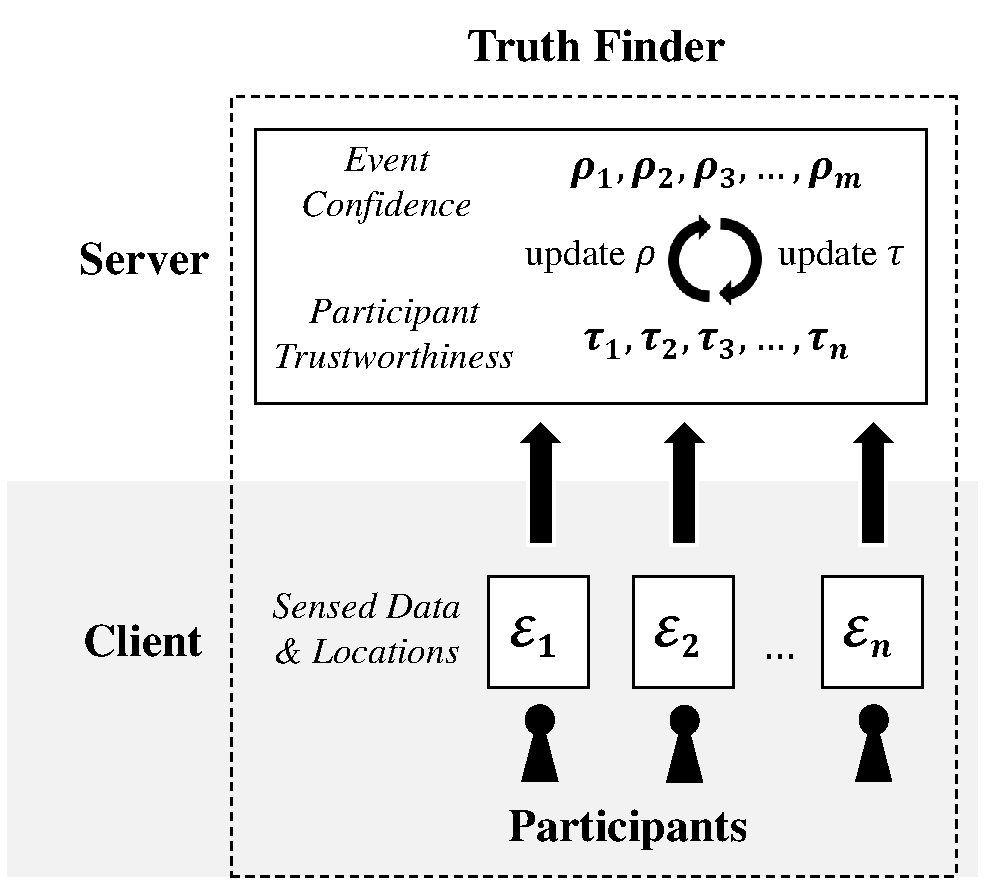
\includegraphics[width=.5\linewidth]{./fig/truthfinder.pdf}
	\caption{Overview of Iterative Truth Discovery}
	\label{fig:truthfinder}
	\vspace{-1em}
\end{figure}


Truth discovery algorithms usually follow an iterative method to calibrate user trustworthiness and data confidence alternatively until convergence \citep{yin2008truth}. Figure~\ref{fig:truthfinder} shows the framework of iterative truth discovery methods. In this paper, for clarity, we assume that sensed data is a binary spatial event. That is, for a specific location, the sensed data can be 1 or 0. Our method can be easily extended to multi-class and continuous-value events (see Appendix). 

As shown in Figure~\ref{fig:truthfinder}, first, participants upload all of their sensed data and locations $\mathcal E_i$  to the central server. The central server would assign an initial trustworthiness score $\tau_i$ to each participant $u_i$ (e.g., 0.9 by assuming that 90\% of the sensed data are accurate). Then, for each sensed event $e_j$, the truth discovery algorithm will calculate its confidence $\rho_j$ (i.e., the probability of $e_j = 1$) by considering the users who have sensed $e_j$ as:
\begin{equation}
\rho_j = F_\rho(\mathcal U_{j,1}, \mathcal U_{j,0})
\label{eq:event_confidence}
\end{equation}
where $\mathcal U_{j,k}$ is the users who have sensed the event $e_j$ with the reported data $k$; $F_\rho$ is an event confidence calculation function which we will elaborate on later. 

With $\rho_j$ for each event $e_j$, we can then update the trustworthiness score $\tau_i$ of each participant $u_i$ by:
\begin{equation}
\tau_i = F_\tau(\mathcal E_{i,1}, \mathcal E_{i,0})
\end{equation}
where $\mathcal E_{i,k}$ is the users' sensed event set with the reported data $k$; $F_\tau$ is a user trustworthiness calculation function which we will elaborate on later. 

Once $\tau_i$ is updated for each user $u_i$, we can continue updating $\rho_j$ for each event $e_j$ according to Eq.~\ref{eq:event_confidence}, and so on, leading to an alternative updating process for both $\tau_i$ and $\rho_j$. This process can be terminated after a fixed number of iterations or until convergence. Next, we elaborate on the common choices of $F_\rho$ and $F_\tau$ in literature.

\textbf{Sum Function}

An intuitive selection of the updating functions of $F_\rho$ and $F_\tau$ is the weighted sum:
\begin{equation}
\rho_j = F_\rho(\mathcal U_{j,1}, \mathcal U_{j,0}) = \frac{\sum_{u_i \in \mathcal U_{j,1}} \tau_i}{\sum_{u_i \in \mathcal U_{j,1}} \tau_i + \sum_{u_k \in \mathcal U_{j,0}} \tau_k}
\label{eq:rho_function_sum}
\end{equation}
\begin{equation}
\tau_i = F_\tau(\mathcal E_{i,1}, \mathcal E_{i,0}) = \frac{\sum_{e_j \in \mathcal E_{i,1}} \rho_j + \sum_{e_k \in \mathcal E_{i,0}} 1-\rho_k}{|\mathcal E_{i,1}|+|\mathcal E_{i,0}|}
\label{eq:tau_function}
\end{equation}

\textbf{Logistic Function}

Another widely used updating function is the Logistic function \citep{yin2008truth}. Its basic idea is seeing every user independently, so that the probability of event happening, i.e., $e_j=1$, can be formulated as:
\begin{equation}
	\rho_j = 1 - \prod_{u_i \in \mathcal U_{j,1}} (1-\tau_i)
\end{equation}
As $1-\tau_i$ may often be small and multiplying many of them may lead to underflow, prior studies proposed to use the logarithm to define a log-trustworthiness score of $u_i$ as \citep{yin2008truth}:
\begin{equation}
	\tau_i^* = - \ln(1-\tau_i)
\end{equation}
Similarly, a log-confidence score of event $e_j$ is defined as:
\begin{equation}
	\rho_j^* = - \ln(1-\rho_i)
\end{equation}
Then, we can infer 
\begin{equation}
	\rho_j^* = \sum_{u_i \in \mathcal U_{j,1}} \tau_i^*
\end{equation}
The above equation does not consider the users' trustworthiness who report $e_j=0$, and thus we refine it:
\begin{equation}
	\rho_j^* = \sum_{u_i \in \mathcal U_{j,1}} \tau_i^* - \sum_{u_k \in \mathcal U_{j,0}} \tau_k^*
\end{equation}
Finally, a logistic function is used to calculate the final confidence $\rho_j$ of event $e_j$ \citep{yin2008truth}:
\begin{equation}
	\rho_j = F_\rho(\mathcal U_{j,1}, \mathcal U_{j,0}) = (1+e^{-\rho_j^*})^{-1}
	\label{eq:rho_function_log}
\end{equation}
$\tau_i$ is updated same as Eq.~\ref{eq:tau_function}.
\section{Method}

Here we discuss the standard retrieve-and-rerank (R\&R) framework for IR (\S{\ref{sec:retrieve_and_rerank}}) and how our proposal fits into it (\S{\ref{sec:cross_encoder_feedback}}). While our approach can be applied to any R\&R framework, we consider a text-based retriever and reranker for simplicity while elaborating our method. A multi-modal R\&R framework is described in \S\ref{sec:multimodal_results}.


\subsection{Retrieve-and-Rerank}
\label{sec:retrieve_and_rerank}
R\&R for IR consists of a first-stage retriever and a second-stage reranker. Modern neural approaches typically use a dual-encoder model as the retriever and a cross-encoder for reranking.  

\paragraph{\textbf{The Retriever}:} The dual-encoder retriever model is based on a Siamese neural network \cite{chicco2021siamese}, containing separate Bert-based \cite{devlin2019bert} encoders $E_Q(.)$ and $E_P(.)$ for the query and the passage, respectively.
Given a query $q$ and a passage $p$, a separate representation is obtained for each, such as the \textsc{cls} output or a pooled representation of the individual token outputs from $E_Q(q)$ and $E_P(p)$. The question-passage similarity $sim(q,p)$ is computed as the dot product of their corresponding representations: query/passage.}
\begin{equation}
    Q_q = Pool(E_Q(q))
\end{equation}
\begin{equation}
    P_p = Pool(E_P(p))
\end{equation}
\begin{equation}\label{eq:sim}
   sim(q,p) = S(Q_q,P_p) = Q_q^TP_p
\end{equation}

Since Eq.~\ref{eq:sim} is decomposable, the representations of all passages in the retrieval corpus can be pre-computed and stored in a dense index \cite{johnson2019billion}. During inference, given a new query, the top $K$ most relevant passages are retrieved from the index via approximate nearest-neighbor search.

\paragraph{\textbf{The Reranker}:} The cross-encoder reranker model uses a Bert-based encoder $E_R(.)$, which takes the query $q$ and a corresponding retrieved passage $p$ together as input and outputs a similarity score. 
A feed-forward layer $F$ is used on top of the \textsc{cls} output from $E_R(.)$ to compute a single logit, which is used as the final reranker score $R(q,p)$. The top $K$ retrieved passages are then ranked based on their corresponding reranker scores.

\begin{equation}
   R(q,p) = F(CLS(E_R(q,p))
\end{equation}


\begin{algorithm}[t]
\caption{\textsc{\textbf{ReFIT}}}
\label{alg4}
\begin{flushleft}
\textbf{Input}: Query $q$ and its representation $Q_q$, retrieved passages $P$ and their representations $\hat{P}$.\newline
\textbf{Output}: Updated query representation $Q_{q,n}$
\end{flushleft}
\begin{algorithmic}[1]
    \State Initialize query vector $Q_{q,0}$ = $Q_q$
    \State Compute reranker distribution $D_{CE}(q,P)$ (Eq.~\ref{eq:d-ce})
    \For{\textit{i in 0 to n}}
        \State Compute retriever distribution $D_{Q_{q,i}}(\hat{P})$ (Eq.~\ref{eq:d-q})
        \State Compute loss $\mathcal{L}$ (Eq.~\ref{eq:loss})
        \State Update $Q_{q,i+1} = Q_{q,i} - \alpha \frac{\partial}{\partial Q_{q,i}}\mathcal{L}$
    \EndFor
    \State return $Q_{q,n}$
\end{algorithmic}
%\vspace{-0.4em}
\end{algorithm}

\subsection{Reranker Relevance Feedback}
\label{sec:cross_encoder_feedback}
The main idea underlying our proposal is to compute an improved query representation for the retriever using feedback from the more powerful reranker.
More specifically, we perform a lightweight inference-time distillation of the reranker's knowledge into a new query vector.

Given an input query $q$ during inference, we use the following output provided by the R\&R pipeline:
\begin{itemize}
   \item Query representation $Q_q$ from the retriever.
    \item Retrieved passages $P = \{p_1, p_2,  ..., p_K\}$ and their representations $\hat{P} = [P_{p_1}, P_{p_1},  ..., P_{p_K}]$ from the retriever. 
    \item The reranking scores $R(q,P) = [R(q,p_1),..., R(q,p_K)]$.
\end{itemize}
Note that $\hat{P}$ above is directly obtained from the passage index and is not computed during inference.

The proposed reranker feedback mechanism begins with using the reranking scores $R(q,P)$ to compute a cross-encoder ranking distribution $D_{CE}(q,P)$ over passages $P$ as follows:

\begin{equation}
D_{CE}(q,P)=\mathrm{softmax}([R(q,p_1), ..., R(q,p_K)])
\label{eq:d-ce}
\end{equation} 

The query and passage representations from the retriever are used to compute a similar distribution $D_{Q_q}(\hat{P})$ over $P$:

\begin{equation}
    D_{Q_q}(\hat{P}) = \mathrm{softmax}([Q_q^TP_{p_1}, ..., Q_q^TP_{p_K}])
    \label{eq:d-q}
\end{equation}

Next, we compute the loss as the KL-divergence between the retriever and reranker distributions:

\begin{equation}
    \mathcal{L} = D_{KL}(D_{CE}(q,P) || D_{Q_q}(\hat{P}))
    \label{eq:loss}
\end{equation}

which is then used to update the query vector via gradient descent. The query vector update process is repeated for $n$ times, where $n$ is a hyper-parameter. 
A schematic description of the process can be found in Algorithm \ref{alg4}. 

Finally, the updated query vector $Q_{q,n}$ is used for a second-stage retrieval from the passage index.  
From dual-encoder retrieval with the updated $Q_{q,n}$, we aim to achieve better recall than with the initial $Q_q$, while obtaining a ranking performance that is comparable with that of the reranker.







\section{Federated Trustworthiness Rank}
\label{sec:trust_ranking}

While FedTruthFinder learns the integrated event truth in a privacy-preserving manner, it brings a challenge in justifying participants' trustworthiness. For example, to incentivize the crowdsensing participants, it is a common strategy to pay the high-trustworthy participants (i.e., high-quality sensing results) with higher incentives. However, in FedTruthFinder, the sensing quality of each participant, i.e., the trustworthiness score $\tau_i$ is kept at each participant side and unknown to the server. Hence, how to assess participants' trustworthiness is required and challenging for FedTruthFinder.

In this section, we first illustrate a concrete case to describe that $\tau_i$ cannot be directly known to the server, otherwise the server may infer which event $u_i$ has sensed. As $\tau_i$ cannot be known to the server, we then design a secure ranking algorithm to let the server know every participant $u_i$'s ranking position of $\tau_i$ among all the participants without leaking $\tau_i$. Based on the ranked positions, the crowdsensing organizer can enable certain trustworthiness-aware incentive mechanisms, e.g., rewarding high-position participants with bonus, which can incentivize participants to compete with each other to get more high-quality sensed data \citep{Reddy2010ExaminingMF}.

\subsection{Privacy Leakage by Trustworthiness $\tau_i$}

Here, we illustrate an example to show the risk of revealing $\tau_i$ to the server for leaking participant $u_i$'s privacy.

Without the loss of generality, we assume that $u_1$'s $\tau_1 = 0.9$, and other $u_i$'s $\tau_i < 0.9\ (i\not=1)$. Suppose that one event $e_j$'s $\rho_j = 0.9$ after truth discovery, then we can easily infer that $u_1$ has sensed the event $e_j$ and the sensed result is $1$. This reveals the fact that $u_1$ has visited the location of $e_j$, leaking $u_1$'s location privacy.

Hence, participants cannot directly upload their $\tau_i$ to the server for incentive allocation. Next, we design a privacy-preserving method to enable trustworthiness-aware incentive allocation. 

\subsection{Secure Trustworthiness Leader-board}

While revealing $\tau_i$ may leak participants' private information, we propose a secure ranking algorithm to learn a  leader-board regarding participants' trustworthiness for facilitating trustworthiness-aware incentive allocation.

Secure ranking algorithms have been studied for decades; however, prior studies cannot be directly applied in our scenario for two reasons. First, the communication overheads are usually high. Second, prior studies mostly assume that all the network connections are stable for all the parties, but this is unrealistic for crowdsensing. 

Our secure ranking algorithm generally follows the design of \citet{tang2011secure}. However, the original design \citep{tang2011secure} cannot tolerate any participants to lose the network connections. We thus enhance it to ensure that the ranking algorithm can still work when certain participants lose connections.
The major steps of our federated trustworthiness leader-board generation mechanism are:

\textbf{Step 1}. First, we categorize all the participants into $(2t+1)$ groups, and thus each group includes $n/(2t+1)$ participants. We denote $gid(u)$ to refer to the group ID of participant $u$.

\textbf{Step 2}. For each user $u_i$, she shares $\tau_i$, $\tau_i^2$, ... , $\tau_i^{2t+1}$ with $(t+1, 2t+1)$-SSS to all the user groups. Specifically, a user $u_j$ will receive the share piece regarding $gid(u_j)$, denoted as $\tau_{i_1}(gid(u_j))$, $\tau_{i_2}(gid(u_j))$, ... $\tau_{i_{2t+1}}(gid(u_j))$ for $\tau_i$, $\tau_i^2$, ... , $\tau_i^{2t+1}$, respectively.

\textbf{Step 3}. For each user group $g_k$, it generates a random number $r_k (>0)$ and shares $r_k$ with $(t+1, 2t+1)$-SSS to all the user groups. That is, $u_j$ will receive $r_k$'s share regarding $gid(u_j)$, denoted as $r_k(gid(u_j))$.

\textbf{Step 4}. For each participant $u_j$, she calculates the following number with the $\tau_{i_k}(gid(u_j))$ received from $u_i$:
\begin{align}
h_{i}(gid(u_j)) &= \lambda(gid(u_j)) \sum_{k=1}^{2t+1} r_k(gid(u_j)) \tau_{i_k}(gid(u_j)) \\ &= \lambda(gid(u_j)) \gamma(gid(u_j))
\end{align}
where
\[
\left(\begin{array}{ccccc} 
	1 &    1 & 1^2 & ...  & 1^{2t} \\ 
	1 &    2 & 2^2 & ... & 2^{2t}\\
	... & ... & ... & ...& ...\\
	1 & 2t+1 & (2t+1)^2 & ... & (2t+1)^{2t}\\
\end{array}\right)^{-1} 
\]
\[
=\left(\begin{array}{ccccc} 
	\lambda(1) &   \lambda(2) & \lambda(3) & ...  & \lambda(2t+1) \\ 
	... & ... & ... & ...& ...\\
	... & ... & ... & ...& ...\\
	... & ... & ... & ...& ...
\end{array}\right) 
\]


\textbf{Step 5}. For each user group, we randomly select one participant $u_j$ to share $\{h_{i}(gid(u_j))| i \in [1,n]\}$ with $(t+1, n)$-SSS to all the $n$ participants. Each user $u_k$'s received shares from all the groups are denoted as $\{h_i(g, k)| i \in [1,n], g \in [1, 2t+1]\}$.

\textbf{Step 6}. For each participant $u_k$, she computes:
\begin{equation}
h'_i(k) = \sum_{g=1}^{2t+1} h_i(g, k), \quad \forall i \in [1,n]
\end{equation}
Each $u_k$ sends $\{h'_i(k)| i\in[1,n]\}$ to the server.

\textbf{Step 7}. After receiving at least $t+1$ participants' $\{h'_i(k)| i\in[1,n]\}$, the server can recover:
\begin{equation}
	h_i = \sum_{k=1}^{2t+1} r_k \tau_i^k, \quad \forall i \in [1,n]
\end{equation}

\textbf{Step 8}. The server ranks $u_i$ according to $h_i$ and the ranked list is the leader-board regarding trustworthiness $\tau_i$.

Note that same as $\rho$-computation, we do not need to establish the peer-to-peer communication channels between every two participant clients and can use the crowdsensing server for coordination. To avoid redundancy, readers can refer to Sec.~\ref{subsub:server_coordination} for details.

\textbf{Remark on our novelty}. The key improvement of our secure ranking algorithm compared to \citet{tang2011secure} is the enhanced robustness against participants' connection loss. In \citet{tang2011secure}, every participant holds a $r_i$ and we will randomly select $2t+1$ participants to share their $r_i$ (Step 3) and $h_i$ (Step 5). This process is easy to break if a selected online user (Step 3) loses the connection in Step 5. Our proposed algorithm first constructs user groups so that we only need at least one participant online in each group for both Step 3 and 5, reducing the failure possibility incurred by connection loss. It is worth noting that this algorithm can not only rank crowdsensing participants' trustworthiness, but also be applied to many other applications when privacy-preserving data ranking is needed under unstable network connections.

\textbf{Remark on the ranked measurements}. In the previous algorithm description, we suppose that $\tau_i$ needs to be ranked. In practice, crowdsensing organizers can use the same secure ranking mechanism to rank other key measurements of participants (e.g., the number of sensed events) to design better incentive mechanisms or participant recruitment strategies.

\subsection{Theoretical Analysis}
\label{sub:theoretical_analysis_2}

All the proofs are illustrated in Appendix.

\subsubsection{Correctness} We first prove the correctness of our algorithm.

\vspace{+.5em}
\textbf{Lemma 5.1}. $\sum_{k=1}^{2t+1} r_k(x)\tau_{i_k}(x)$ can be represented as:
$$h_{i}+a_{i1}x+a_{i2}x^2+...+a_{i2t}x^{2t}$$
where $h_i=\sum_{k=1}^{2t+1} r_k\tau_i^k$. \citep{tang2011secure}
 
\vspace{+.5em}
\textbf{Theorem 5.1}. With $t+1$ participants' $h'_i(k)$, we can recover $h_i$.

\begin{figure*}[t!]%[tbhp]
	\centering
		\begin{subfigure}[t]{.325\linewidth}
			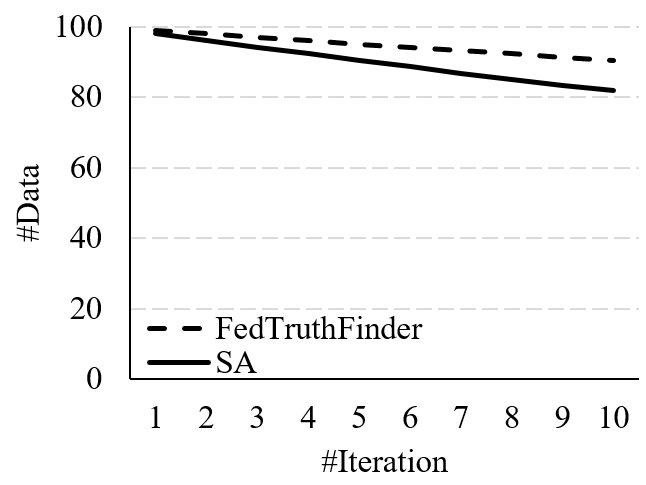
\includegraphics[width=1\linewidth]{./fig/data_num_cl0.01.PNG}
			\caption{$p_l=0.01$}
			\label{fig:cl0.01}
		\end{subfigure}
		\begin{subfigure}[t]{.325\linewidth}
			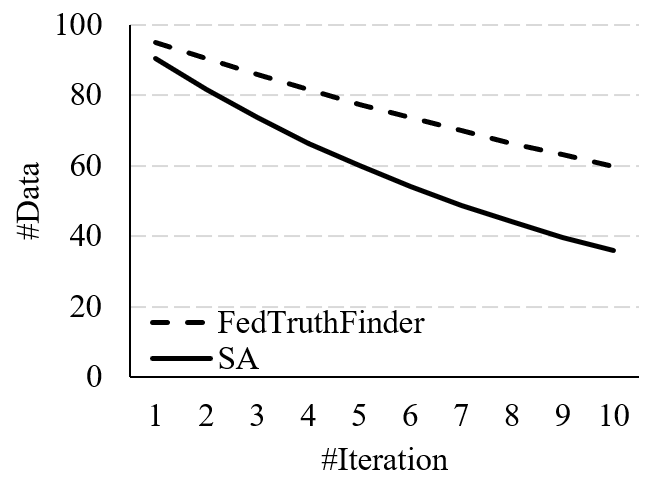
\includegraphics[width=1\linewidth]{./fig/data_num_cl0.05.PNG}
			\caption{$p_l=0.05$}
			\label{fig:chicago}
		\end{subfigure}
		\begin{subfigure}[t]{.325\linewidth}
			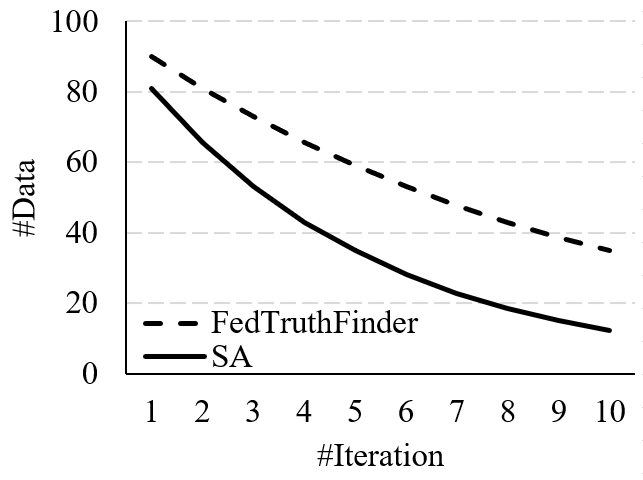
\includegraphics[width=1\linewidth]{./fig/data_num_cl0.1.PNG}
			\caption{$p_l=0.1$}
			\label{fig:dc}
		\end{subfigure}
		\caption{Number of data for each event's truth discovery by iterations.}
		\label{fig:num_sensed_data}
\end{figure*}

\begin{figure*}
	\centering
		\begin{subfigure}[t]{.3\linewidth}
			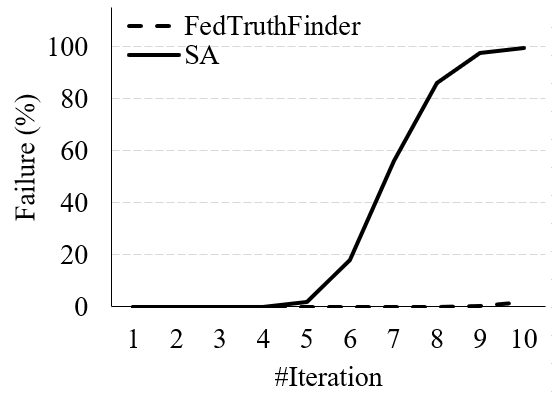
\includegraphics[width=1\linewidth]{./fig/failure_cl0.05.PNG}
			\caption{$p_l=0.05$}
		\end{subfigure}
		\begin{subfigure}[t]{.3\linewidth}
			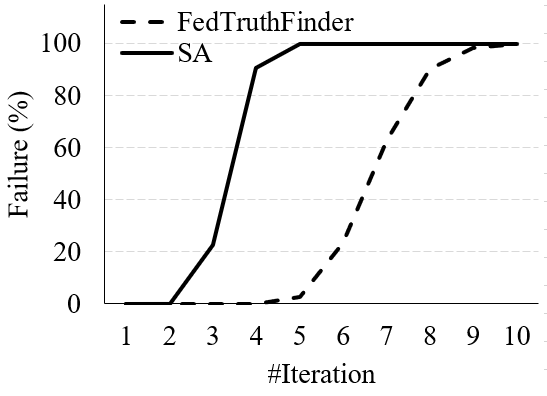
\includegraphics[width=1\linewidth]{./fig/failure_cl0.1.PNG}
			\caption{$p_l=0.1$}
		\end{subfigure}
		\caption{Failure probability of truth discovery.}
		\label{fig:failure}
\end{figure*}

\vspace{+.5em}
\textbf{Theorem 5.2}. Ranking $h_i$ is equivalent to ranking $\tau_i$.


\subsubsection{Robustness to Connection Loss} We analyze how our secure ranking algorithm can tolerate connection losses. We assume that before Step 2, there is no user connection loss.\footnote{If $u_i$ loses the connection in Step 2 and cannot share $\tau_i^k$ with SSS, then there is no way to rank $u_i$'s position because the server has no $u_i$'s information.}

\vspace{+.5em}
\textbf{Theorem 5.3}. To finish Step 3-5, there needs at least one user online for each group. Suppose that every user has $p_l$ probability to lose connection and there are $n$ users, the success probability $\ge (1-p_l^{\lfloor n/(2t+1) \rfloor})^{2t+1}$.


\vspace{+.5em}
\textbf{Theorem 5.4}. To finish Step 6-8, $\ge t+1$ users need to be online.



\subsubsection{Security} Here, we analyze the security of our mechanism.

\vspace{+.5em}
\textbf{Theorem 5.5} If there are no more than $t$ collusive participants, then these participants cannot recover all the other users' $\tau_i$.






\subsubsection{Complexity} We analyze the algorithm from communication and computation complexity perspectives for participant clients.

\textbf{Communication Complexity - $O(tn)$}. In Step 2, the communication overhead of one participant to send $\tau_i,\tau_i^2,...,\tau_i^{2t+1}$ is $O(t^2)$, while each user received data is $O(tn)$. In Step 3, the complexity is $O(t)$. In Step 5, for sending data, the complexity is $O(n)$; for receiving data, the complexity is $O(tn)$. In Step 7, the complexity is $O(n)$. Combing them together, the communication complexity of the whole process is $O(tn)$ as $t<n$.


\textbf{Computation Complexity - $O(tn)$}. The main computation processes of each client include (1) calculating secret shares for $\tau_i,\tau_i^2,...,\tau_i^{2t+1}$ with $(t+1, 2t+1)$-SSS in Step 2, which is $O(t^2)$, (2) calculating secret shares of $r_k$ in Step 3, which is $O(t)$, (3) computing  $h_i$ in Step 4, which is $O(tn)$, and (4) calculating $h_i'$ in Step 6, which is $O(tn)$. Hence, the final computation complexity is $O(tn)$.

\subsection{Experimental Setup}
In this section, we empirically evaluate the effectiveness and interpretability of the proposed~\dname~on both
simulation and real-world datasets.
For interpretability, we focus on whether the algorithm can uncover the causal relationships inherent in the knowledge graph.


\subsubsection{\textbf{Baselines}}
% The aim of this experiment was to evaluate both the effectiveness and interpretability of the existing methods and our approach.
% In this paper, we design a causal rule-based prediction algorithm mainly for application scenarios that require explainability.
To evaluate the interpretability of the algorithms, we select four rule-based methods
that can conduct link prediction and generate explainable rules.
To make a fair comparison, the inference rules, obtained from different algorithms, are used to conduct the link prediction task based on the same prediction equations.
This approach can also help us observe the impact of different rules on the link prediction task.
For a complete evaluation of the effectiveness of the proposed approach, we also compute the LP performance of TuckER\cite{balazevic2019tucker}, one representation-based method which has the best overall performance among the representation-based methods across different datasets\cite{rossi2021knowledge}.
All baselines are listed in the following:
\begin{itemize}
\item[1)] AMIE+\cite{galarraga2015fast}, an efficient  top-down method to discover the interpretable rules.
\item[2)] AnyBURL\cite{meilicke2019anytime}, a bottom-up approach to mine the logical rule.
\item[3)] Neural-LP\cite{yang2017differentiable}, an end-to-end differentiable model to learn the first-order logical rule.
\item[4)] RNNLogic\cite{qu2020rnnlogic}, an EM-based algorithm to learn the rule generator and the reasoning predictor iteratively.
\item[5)] TuckER\cite{balazevic2019tucker},  a linear model based on Tucker
decomposition of the binary tensor representation of knowledge graph triples.
\end{itemize}





\subsubsection{\textbf{Datasets}}
To quantitatively evaluate the effectiveness of the algorithm in discovering causal knowledge, we construct a simulation dataset owing to a lack of groundtruth of real datasets.
Douban and Hetionet~\cite{himmelstein2017systematic} are selected as our real datasets on which we perform two link prediction tasks, movie rating prediction and drug repurposing, respectively.
Here we provide more details for these datasets, and their statistics are shown in Table~\ref{tab:dataset_statistics}.

% \begin{figure}[t]
% \vspace{0cm}
% \centering
% 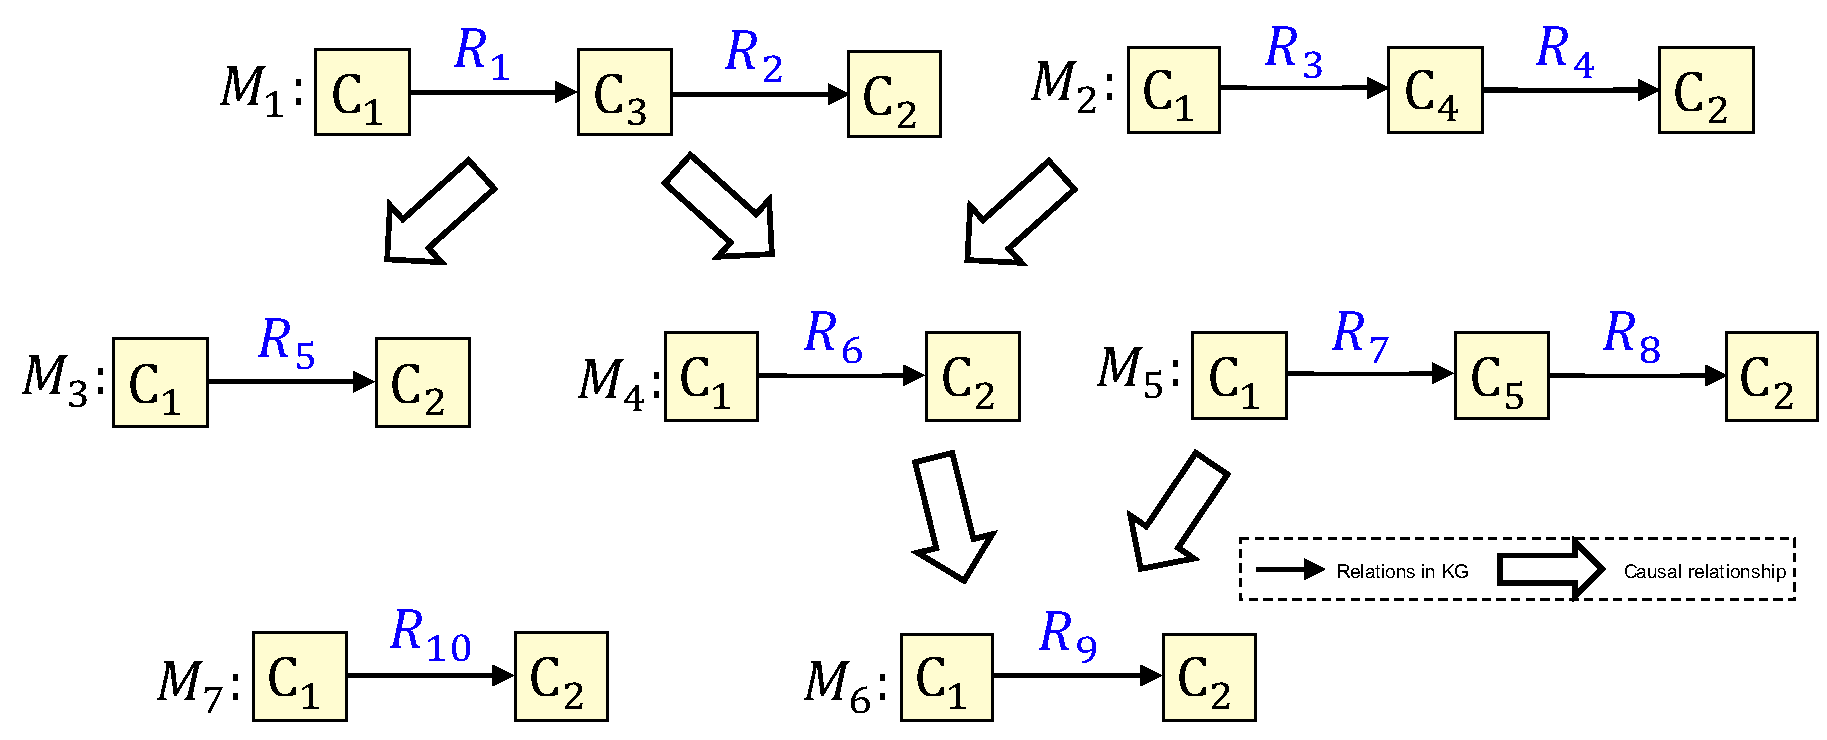
\includegraphics[width=8.5cm]{./figures/simulation.pdf}
% \caption{ The causal graph used to generate simulated knowledge graphs.}
% \label{fig:toy_example}
% \end{figure}

\begin{table}[t]
\centering
\caption{Dataset statistics of all the experiments.}
\label{tab:dataset_statistics}
% \vspace{-2pt}
\scalebox{1}{
\begin{tabular}{c|ccc}
\hline
   & \textbf{\#Triplets} & \textbf{\#Relations} & \textbf{\#Entities}  \\
\hline
\textbf{Simulation} & 6,095 & 5 & 1,590\\
\textbf{Douban Movie Rate} & 28,356 & 12 & 3,007 \\
\textbf{Hetionet} & 174,941 & 20 & 32,056 \\
\hline
\end{tabular}
}
\end{table}

\noindent
{\bf Simulation dataset.}
We generate simulated KGs based on a toy causal model specified in Fig.~\ref{fig:simulation}, which includes three concepts and five relations.
In particular, we design the causal mechanisms in KG via a probabilistic model.
The root nodes ($X_1$, $X_4$) in the causal graph are generated via Bernoulli distributions, whose probability mass function is $f_X(x)=p^x(1-p)^{1-x}$.
Moreover, the non-root nodes ($X_2$, $X_3$) are generated via the conditional probability distributions, which are Bernoulli distributions, given the parent node ($X_1$).
To maintain a stable causal mechanism, the parameters of conditional distributions are constant in training and testing, as shown in Table~\ref{tab:simulation_set}.
In the out-of-distribution paragraph, we will introduce the parameters of root nodes in training and testing.


\begin{figure}[h]
\centering
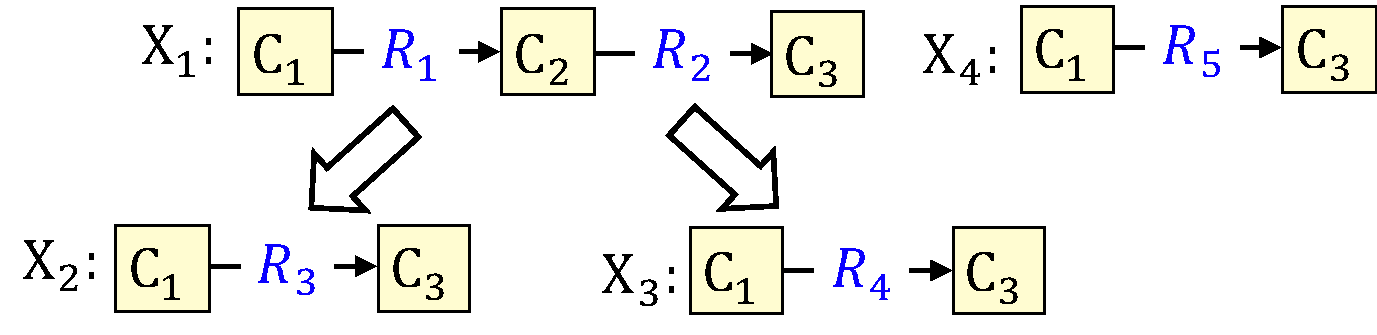
\includegraphics[width=7cm]{submissions/causal-meta-knowledge/figures/simulationv4.pdf}
\caption{The causal graph of relation paths, based on which the simulated KGs are generated .}
\label{fig:simulation}
% \vspace{-2pt}
\end{figure}

\begin{table}[h]
\caption{The parameters of conditional distributions.}
%\vspace{5pt}
\label{tab:simulation_set}
\centering
\scalebox{1}{
\begin{tabular}{c|cccc}
\hline
Conditions & $X_2|X_1=1$ & $X_2|X_1=0$ & $X_3|X_1=1$ & $X_3|X_1=0$ \\
\hline
Parameters & $p$=0.9 & $p$=0.1 & $p$=0.9 & $p$=0.1 \\
\hline
\end{tabular}}
% \vspace{-2pt}
\end{table}
% We generate simulated KGs based on a toy causal model specified in Fig.~\ref{fig:toy_example}, which includes five concepts and ten relations.
% More specifically, given $N$ entities for each concept, the facts containing the relations in the root nodes ($M_1$, $M_2$, $M_7$) of the causal graph are generated via Bernoulli distributions, whose probability mass function is $f(x)=p_r^x(1-p_r)^{1-x}$.
% For example, the entity pair $(e_1,e_3)$, where $e_1 \in \mathcal{E}_{C_1}$ and $e_3 \in \mathcal{E}_{C_3}$, the probability that the fact $<e_1,R_1,e_3> \in \mathcal{G}$ is $p_r$.
% % It means for any entity pair $(e_h,e_t)$, where $e_h \in \mathcal{E}_{C_h},\mathcal{E}_{C_t}$ and $R_i(C_h,C_t) \in \text{KG schema} \mathcal{S}$, the probability that the fact $R_i(e_h,e_t) \in \mathcal{T}$ is $p_r$.
% % we design the conditional  probabilistic distribution in SPRM based on which to sample the entity and facts in KG.
% And the facts in non-root nodes (e.g., $M_3$) are generated via the conditional probability distributions, which are Bernoulli distributions with parameter set $\mathbf{p}_{nr}$, given the facts information of parent node ($M_1$).
% For example, if there is a path instance of $M_1$ between $(e_1,e_3)$, then the probability of the existence of fact $<e_1,R_5,e_3>$ is $p_{M_1=1}$, otherwise is $p_{M_1=0}$.
% \yym{the value of all parameter of $p_nr$}

%


\noindent
{\bf Douban movie rating.}
Douban is a famous Chinese website for movie reviews, where users can rate and comment on any movie.
The rating range is from 1 to 5. A higher rating means that users like movies, while a lower rating means that users have negative feedback on movies.
We collect the real-world data from Douban\footnote{https://www.douban.com/} and construct a dataset (this dataset will be released), whose statistics are shown in Table~\ref{tab:dataset_statistics}.
Commonly, a movie with a score of 4 or 5 is identified as meeting the taste of users.
So we transform the original 5-level rating to a 2-level rating with a threshold of 4.
If the rating score is 4 or 5, the original relation \textit{Rate} is replaced by  \textit{HighRate}
We conduct the link prediction task on the relation \textit{HighRate}.
Because the raw data is too large and the relations between users and movies are very sparse, in this thesis, we first filter the 20 users who have made the most ratings and take the rating history of these users as the set of rating facts for our study.
The facts unrelated to the rating are also included in our experimental data.

\noindent
{\bf Hetionet}\cite{himmelstein2017systematic}
is a freely available knowledge database that integrates biomedical information from 29 prominent
bioinformatics resources.
Recently, Hetionet was successfully applied to drug repurposing tasks in terms of the link prediction task for relation \texttt{Treats}\cite{himmelstein2017systematic, ratajczak2022task}.

\textit{Why do we choose those two real datasets instead of other commonly used datasets, such as WN18, FB15k?}
In this paper, we focus on link prediction with the help of causal relationships between knowledge graph relations.
The core of causality lies in its asymmetry.
The commonly used KGs for link prediction algorithms contain many symmetrical relationships, e,g., \textit{hypernym} and \textit{hyponym} in WN18.
These symmetrical relationships may help with the link prediction task, but they go against the basic idea that causality is a one-way relationship.
We, therefore, chose datasets with specific application scenarios and rich causal semantics.

\subsubsection{\textbf{Metrics.}}
\textbf{For link prediction}, we employ the commonly used metrics mean reciprocal rank (MRR) and Hits@k~\cite{rossi2021knowledge,balazevic2019tucker,bordes2013translating}.
\begin{equation}
\label{eq:mrr}
\begin{aligned}
M R R=\frac{1}{|Q|} \sum_{q \in Q} \frac{1}{q}
\end{aligned}
\end{equation}

\begin{equation}
\label{eq:hitk}
\begin{aligned}
Hit@K=\frac{|\{q \in Q: q \leq K\}|}{|Q|}
\end{aligned}
\end{equation}
where $Q$ is the rank results, for each $q_i \in Q$ is the ranking of the desired results in the $i$-th query $(?,R_h,e_t)$.
In the case of ties in the calculation of $Q$, we use the mean rank to avoid misleading results\cite{rossi2021knowledge,ruffinelli2020you}.
% Common values for $K$ are 1, 3, 5, 10, we use $K=5$ in this paper.
Both MRR and His@k are the higher, the better.

\noindent
\textbf{The interpretability of causal rules} on the simulation dataset can be understood as the consistency between the mined causal rules and the actual causal structure.
Therefore, we evaluate baselines and our approach on the simulation dataset using precision, recall, and structural Hamming distance (SHD) as the evaluation metrics, which are commonly used evaluation metrics in causal structure discovery studies~\cite{zheng2018dags,zheng2020learning}.
% Since the performance of causal rule discovery is the foundation of our link prediction method.

\begin{equation}
\label{eq:precision}
\begin{aligned}
Precision=\frac{\# TFR}{\#FR};Recall=\frac{\# TFR}{\#ATR}
\end{aligned}
\end{equation}
Where $\#TFR$ is the number of right causal relationships discovered by an algorithm, $\#FR$ is the number of causal relationships discovered by an algorithm, and $\#ATR$ is the number of all causal relationships.
Both precision and recall are the higher, the better.
SHD calculates the difference between the learned graph and the ground truth graph by the number of edge insertions, deletions, or flips required to transform one graph into another.
The lower the SHD, the better.

\subsubsection{\textbf{Out-of-Distribution Link Prediction}}
Traditional machine learning methods are designed based on the assumption of independent and identically distributed (I.I.D) data.
This assumption means the training and test data come from the same distribution. However, the distribution of test data may alter due to changes in the test environment; such tasks are referred to as OoD tasks.
Traditional algorithms perform poorly on generalization problems due to the violation of I.I.D assumption.
Causality is seen as a stable inference mechanism in many research works on generalization problems.
So, in this work, we provide an out-of-distribution generalization task for the knowledge link prediction task for the first time.
On the one hand, the effect of causal metaknowledge on this task can be measured, and on the other, the performance of existing algorithms can be looked at.
We also evaluate the performance of the algorithms on I.I.D link prediction tasks.

In this paper, we design two OoD experimental scenarios.

\noindent
(1) \textit{Simulation dataset}:
We evaluate the link prediction performance under I.I.D and OoD settings, where the triples of root node $X_1$ are generated in testing under the same and different parameters with training.
In the training and I.I.D testing datasets, $p_{X_1}=0.5$.
In the OoD testing datasets, $p_{X_1} \in \{0.2,0.9\}$.
For $X_4$, $p_{X_4}$ maintains $0.9$ in training and testing.
The facts of the KGs are split into three parts:\textit{train}, \textit{test info}, and \textit{test}.
The facts in \textit{train} are used to learn the rule.
The effectiveness of the learned rule is assessed via the link prediction task on $R_3$.
The \textit{test info} part includes facts of new entities (did not appear in \textit{train}) on $R_1, R_2, R_4, R_5$, and \textit{test} part includes the queried facts on $R_3$.

\noindent
(2)\textit{Real datasets}:
It is impossible to explicitly change the data distribution since real data distribution is inaccessible for real datasets.
Recent research\cite{tang2020investigating,wu2021self} has suggested that graph models are biased towards nodes with larger degrees, which causes the bad performance of low-degree nodes in the test.
Therefore we construct the OoD datasets based on degree shift.
Specifically, given a query task $(?,R_h,e_t)$, we calculate the \textit{median} of degree\footnote{In this paper, we use the term "degree" to stand for the sum of in and out degrees} of known entities $e_t$ belonging to the triples $(e_h,R_h,e_t)$ in the training.
Then we bin the test queries by the degrees of the known entities $e_t$.
The degree range in each bucket is decided based on the sample size balance.
The test queries in the bucket, which the training median falls in, can be treated as the I.I.D test samples.
Others are the OoD samples.
The I.I.D bucket is labeled with $*$ in Table~\ref{tab:douban-mrr} and Table~\ref{tab:hetionet-mrr}.





\subsection{Performance of Link prediction task in Out-of-Distrition Settings}

\noindent
\textbf{Results on simulations.}
For the simulation dataset, we construct a OoD setting named as covariance shift, by changing the probability distribution of the root nodes in the test phase.
Table~\ref{tab:simulation_result} presents the methods in performance and demonstrates the effectiveness of the proposed \dname.
In particular, \dname~outperforms the baseline models under all metrics except the Hits@10 under I.I.D setting. This shows our method can give a stable and high-quality result, especially in the OOD setting.
Besides, compared with the baselines, the proposed \dname~ perform significantly better at the Hits@1 metric (at least 25\% absolute improvements that the second place under all settings), which suggests the our method are more suitable for scenarios with strict performance requirements, and this feature may achieved by the removal of association-based rules.

\begin{table}[h]
\caption{The results of link prediction on simulation datasets.}
\centering
\label{tab:simulation_result}
\scalebox{1.2}{
\begin{tabular}{c|c|l|cccc}
\hline
 \multirow{2}{*}{\textbf{Settings}}& \multirow{2}{*}{$\mathbf{p_{X_1}}$} & \multirow{2}{*}{\textbf{Method}} & \multirow{2}{*}{\textbf{MRR}} & \multicolumn{3}{c}{\textbf{Hits}} \\ \cline{5-7}
& & & &\textbf{@10} & \textbf{@3} & \textbf{@1} \\ \hline
\multirow{4}{*}{I.I.D} & \multirow{4}{*}{0.5}
& AMIE+ & 0.87 & \textbf{98.99} & 94.95 & 78.79\\
&  & AnyBURL & 0.87 &\textbf{98.99}&94.95 &78.79\\
&  & Neural-LP &  0.80 & \textbf{98.99} & 92.42& 66.16\\
& & RNNLogic & 0.87 & \textbf{98.99} & 94.95 & 78.79\\
&& \dname & \textbf{0.94} & 98.48&\textbf{97.98} &\textbf{90.91}\\

 \hline
\multirow{4}{*}{OOD} & \multirow{4}{*}{0.2}
& AMIE+ & 0.875 & 96.91 & 93.81 & 81.44 \\
&  & AnyBURL &  0.875 & 96.91&93.81 & 81.44\\
& & Neural-LP & 0.68 & 98.97 & 79.38 & 50.51\\
& & RNNLogic & 0.875 & 96.91 & 93.81 & 81.44 \\
&& \dname & \textbf{0.99} & \textbf{100}&\textbf{100} &\textbf{99.97}\\
 \hline
 \multirow{4}{*}{OOD} & \multirow{4}{*}{0.9}
& AMIE+ & 0.91 & \textbf{100} & 96.34 & 85.67 \\
&  & AnyBURL &  0.91 &\textbf{100} & 96.34 & 85.67\\
& & Neural-LP & 0.88 & \textbf{100} & 96.95 & 79.57\\
& & RNNLogic & 0.91 & \textbf{100} & 96.34 & 85.67 \\
&& \dname & \textbf{0.99} &  \textbf{100}& \textbf{99.70} & \textbf{99.09}\\
 \hline
\end{tabular}
}
\end{table}

% Also we considered the effect of different score functions on the link prediction performance.
% The results are shown in Tab.~\ref{tab:simulation_result}, and  can find that our method also works well for the simulated data, especially under OoD settings. Specifically, our model gets the best MRR and Hit@1 results, while AMIE+ and AnyBURL are the best methods for Hit@5 and Hit@10 for I.I.D setting. This may be because they tend to discover more rules, while our method aims to identity the causality more accurately, so fewer links are predicted.
% For OoD data, the proposed method surpasses all baseline models on all metrics, which fully support our motivation: building a link prediction algorithm with strong generalization ability.

% Overall, our method performs best for all three datasets. Also note although some baselines get the best results under some specific settings, they can not maintain a good performance for other settings or metrics. For example, TuckER gets the best MRR under 0-5 degree range, while performs worst with 30-60 degree range on Douban movie rating dataset. By contrast, the proposed CMLP can achieve best or competitive results for all settings.

% \yym{Prior systems for generating conjectures have either contributed genuinely useful research conjectures9 via methods that do not easily generalize to other mathematical areas10, or have dem- onstrated novel, general methods for finding conjectures11 that have not yet yielded mathematically valuable results.}


% \begin{table}[h]
% \caption{The results of link prediction on simulation datasets.}
% \centering
% \label{tab:simulation_result}
% \scalebox{1}{
% \begin{tabular}{c|c|l|cccc}
% \hline
%  \multirow{2}{*}{\textbf{Settings}}& \multirow{2}{*}{$\mathbf{p_{r}}$} & \multirow{2}{*}{\textbf{Method}} & \multirow{2}{*}{\textbf{MRR}} & \multicolumn{3}{c}{\textbf{Hits}} \\ \cline{5-7}
% & & & &\textbf{@1} & \textbf{@5} & \textbf{@10} \\ \hline
% \multirow{5}{*}{I.I.D} & \multirow{5}{*}{0.3}
% & AMIE+ & 0.734 & 0.589 & \textbf{0.948} & \textbf{1}\\
% &  & AnyBURL & 0.733 & 0.589 & \textbf{0.948} & \textbf{1}\\
% &  & Neural-LP &  0.58 & 0.41 & 0.743 & 0.769\\
% &  & RNNLogic &  0.603 & 0.461 & 0.666 & 0.666\\
% & & \dname & \textbf{0.785} & \textbf{0.692} & 0.897 & 0.897 \\

% %  \hline
% % \multirow{5}{*}{OOD} & \multirow{5}{*}{0.1}
% % & AMIE+ & 0.73 & 0.538 & \textbf{0.846} & \textbf{0.846} \\
% % &  & AnyBURL &  \textbf{0.782} & \textbf{0.615} & \textbf{0.846} & \textbf{0.846} \\
% % & & Neural-LP & 0.673 & 0.461 & 0.769 & 0.769\\
% % & & RNNLogic & 0.611 & 0.307 & 0.538 & 0.538\\
% % && \dname & 0.692 & 0.538 & 0.692 & 0.692\\
%  \hline
%  \multirow{5}{*}{OOD} & \multirow{5}{*}{0.8}
% & AMIE+ & 0.891 & 0.843 & \textbf{0.98} & \textbf{1} \\
% &  & AnyBURL &  0.893 & 0.843 & \textbf{0.98} & \textbf{1}\\
% & & Neural-LP & 0.885 & 0.843 & 0.941 & 0.98\\
% & & RNNLogic & 0.853 & 0.803 & 0.882 & 0.882\\
% && \dname & \textbf{0.909} &  \textbf{0.862} & \textbf{0.98} & \textbf{1}\\
%  \hline
% \end{tabular}
% }
% \end{table}
\noindent
\textbf{Results for Douban movie rating.}
Since we filtered the users of the Douban data, and the discrepancies of the degrees of experimental user nodes are close to each other.
Therefore, in this experiment, to construct the OoD scenario, we adopt the head prediction (? , HighRate, Movie), predicting the set of users who gave high ratings to movies.
Further, we bucketed the movie nodes in the test data according to their degree in the training data to observe the performance of the algorithm under different node prevalence.
The MRR and Hits@5 results shown in
Tab.~\ref{tab:douban-mrr} shows that the proposed CMLP get the best performance in the all OoD settings.
Especially, at least 25.8\% and 29.3 \% relative improvements that the second place on the MRR and Hits@5, respectively.
In the I.I.D setting, ~\dname~gets the second place on both MRR and Hits@5, lower than the representation-based method TuckER.
These results illustrate that for movie
rating datasets, the rules learned by our method can capture more general user preferences and give relatively accurate rating predictions for movies that are in different popularity.





% sum query head
\begin{table}[]
\centering
\caption{MRR (left) and Hits@5 (right) for Douban movie rating. The * marks columns that contain the I.I.D results. Other columns contain OoD results.}
\label{tab:douban-mrr}
\scalebox{1.2}{
\begin{tabular}{c|ccccc}
\hline
\multirow{2}{*}{\textbf{Methods}} & \multicolumn{4}{c}{\textbf{Degree Range}} \\ \cline{2-5}
          & \textbf{0-21*}   & \textbf{21-31}   & \textbf{31-39} & \textbf{39-60} \\ \hline
AMIE+     & 0.120 & 0.205 & 0.261 & 0.395 \\
AnyBURL   & 0.125 & 0.182  & 0.231 & 0.373 \\
Neural-LP & 0.078 & 0.097  & 0.126 & 0.217 \\
RNNLogic  & 0.072 & 0.086  & 0.097 & 0.161 \\
TuckER    & \textbf{0.287} & 0.186  &  0.186 & 0.149 \\
\dname      & 0.251 & \textbf{0.343}  & \textbf{0.392} & \textbf{0.497}\\ \hline
\end{tabular}
\quad
\begin{tabular}{c|ccccc}
\hline
\multirow{2}{*}{\textbf{Methods}} & \multicolumn{4}{c}{\textbf{Degree Range}} \\ \cline{2-5}
         & \textbf{0-21*}    & \textbf{21-31}   & \textbf{31-39} & \textbf{39-60}  \\ \hline
AMIE+        & 13.7 &30.7  & 39.4  & 68.3  \\
AnyBURL      & 15.1  & 26.0  & 33.2 & 64.6  \\
Neural-LP    & 0.1      & 0.6     & 3.4     & 60.0 \\
RNNLogic     & 1.6    & 4.7  & 7.2 & 13.5  \\
TuckER     & \textbf{50.3}   & 31.9   & 28.2  &  21.5 \\
\dname     & 40.9  & \textbf{60.0}  & \textbf{68.1} & \textbf{88.3}  \\ \hline
\end{tabular}}
\end{table}


% \begin{table}[]

% \caption{Hits@5 for Douban movie rating. The * marks columns that contain the I.I.D results. Other columns contain OoD results.}
% \label{tab:douban-hits1}
% \begin{tabular}{c|ccccc}
% \hline
% \multirow{2}{*}{\textbf{Methods}} & \multicolumn{4}{c}{\textbf{Degree Range}} \\ \cline{2-5}
%          & \textbf{0-21*}    & \textbf{21-31}   & \textbf{31-39} & \textbf{39-60}  \\ \hline
% AMIE+        & 13.7 &30.7  & 39.4  & 68.3  \\
% AnyBURL      & 15.1  & 26.0  & 33.2 & 64.6  \\
% Neural-LP    & 0.1      & 0.6     & 3.4     & 60.0 \\
% RNNLogic     & 1.6    & 4.7  & 7.2 & 13.5  \\
% TuckER     & \textbf{50.3}   & 31.9   & 28.2  &  21.5 \\
% \dname     & 40.9  & \textbf{60.0}  & \textbf{68.1} & \textbf{88.3}  \\ \hline
% \end{tabular}
% \end{table}

\noindent
\textbf{Results for drug repurposing on Hetionet.}
Consistent with the traditional setup of drug redirection, on Hetionet, we also use head predition (?, Treat, Disease), which is giving a Disease to predict new drugs. We also observe the performance of the algorithm under this task by bucketing for Disease node degrees.
Tab.~\ref{tab:hetionet-mrr} reports the MRR and Hits@5 on this dataset, and we can find that: our CMLP performs significantly better than other baselines on low-degree diseases (0-17), while AMIE+ and AnyBURL get better results on low-degree diseases (17-100).
These results indicate that our method can give more accurate drug discovery results for diseases with relatively low information.
And for diseases with richer information, the correlation-based inference rules give more accurate drug prediction.


\begin{table}[]
\centering
\caption{MRR(left) and Hits@5(right) for drug repurposing on Hetionet. The * marks columns that contain the I.I.D results. Other columns contain OoD results.}
\label{tab:hetionet-mrr}
\scalebox{1.2}{
\begin{tabular}{c|ccccc}
\hline
\multirow{2}{*}{\textbf{Methods}} & \multicolumn{4}{c}{\textbf{Degree Range}} \\ \cline{2-5}
    & \textbf{0-8*}    & \textbf{8-17}   & \textbf{17-31}  & \textbf{31-100} \\ \hline
AMIE+   & 0.103  & 0.085  & \textbf{0.132}  & 0.065 \\
AnyBURL  & 0.116   & 0.189  & 0.090  & \textbf{0.188} \\
Neural-LP & 0.027  & 0.014  & 0.009  & 0.009 \\
RNNLogic & 0.07  & 0.021  & 0.029  & 0.012 \\
TuckER  &  0.044  & 0.022    & 0.083   &  0.015 \\
\dname  & \textbf{0.248}  & \textbf{0.208}  & 0.095 & 0.093 \\ \hline
\end{tabular}
\quad
\begin{tabular}{c|cccc}
\hline
\multirow{2}{*}{\textbf{Methods}} & \multicolumn{4}{c}{\textbf{Degree Range}} \\ \cline{2-5}
  & \textbf{0-8*}    & \textbf{8-17}   & \textbf{17-31}  & \textbf{31-100} \\
  \hline
AMIE+      & 13.2  & 11.3  & \textbf{22.5} & 13.2  \\
AnyBURL     & 15.8  & \textbf{25.0}  & 9.6  & \textbf{23.7}   \\
Neural-LP   & 5.3      & 0     & 0      & 0      \\
RNNLogic  & 7.9  & 0  & 3.2      & 0      \\
TuckER    &  3.1   & 5.9  &  10.7  &  3.2   \\
\dname     & \textbf{26.31}  & \textbf{25.0} & 16.1 & 13.1  \\ \hline
\end{tabular}}
\end{table}

% \begin{table}[]

% \caption{MRR for drug repurposing on Hetionet. The * marks the range in which the mean of the training data falls.}
% \label{tab:hetionet-mrr}
% \begin{tabular}{c|ccccc}
% \hline
% \multirow{2}{*}{\textbf{Methods}} & \multicolumn{3}{c}{\textbf{Degree Range}} \\ \cline{2-4}
%     & \textbf{0-5}    & \textbf{5-15*}   & \textbf{15-30}   \\ \hline
% AMIE+   & 0.277  & 0.103  & 0.126   \\
% AnyBURL  & 0.28   & 0.177  & 0.134  \\
% Neural-LP & 0.036  & 0.016  & 0.011  \\
% RNNLogic & 0.149  & 0.038  & 0.023   \\
% TuckER  &  0.085  & 0.021    & 0.078    \\
% \dname  & \textbf{0.329}  & \textbf{0.327}  & \textbf{0.261} \\ \hline
% \end{tabular}
% \end{table}

% \begin{table}[]

% \caption{Hits@5 for drug repurposing on Hetionet. The * marks columns that contain the I.I.D results. Other columns contain OoD results.}
% \label{tab:hetionet-hits1}
% \begin{tabular}{c|cccc}
% \hline
% \multirow{2}{*}{\textbf{Methods}} & \multicolumn{4}{c}{\textbf{Degree Range}} \\ \cline{2-5}
%   & \textbf{0-8*}    & \textbf{8-17}   & \textbf{17-31}  & \textbf{31-100} \\
%   \hline
% AMIE+      & 13.2  & 11.3  & \textbf{22.5} & 13.2  \\
% AnyBURL     & 15.8  & \textbf{25.0}  & 9.6  & \textbf{23.7}   \\
% Neural-LP   & 5.3      & 0     & 0      & 0      \\
% RNNLogic  & 7.9  & 0  & 3.2      & 0      \\
% TuckER    &  3.1   & 5.9  &  10.7  &  3.2   \\
% \dname     & \textbf{26.31}  & \textbf{25.0} & 16.1 & 13.1  \\ \hline
% \end{tabular}
% \end{table}

% \begin{table}[]

% \caption{Hits@1 for drug repurposing on Hetionet. The * marks the range in which the mean of the training data falls.}
% \label{tab:hetionet-hits1}
% \begin{tabular}{c|cccc}
% \hline
% \multirow{2}{*}{\textbf{Methods}} & \multicolumn{3}{c}{\textbf{Degree Range}} \\ \cline{2-4}
%   & \textbf{0-5}    & \textbf{5-15*}  & \textbf{15-30}   \\ \hline
% AMIE+      & 0.111  & 0.02  & 0.027   \\
% AnyBURL     & 0.111  & 0.06  & 0.027     \\
% Neural-LP   & 0      & 0     & 0            \\
% RNNLogic  & 0.055  & 0.02  & 0          \\
% TuckER    &  0.071   & 0  &  0.064    \\
% \dname     & \textbf{0.166}  & \textbf{0.14}  & \textbf{0.138}   \\ \hline
% \end{tabular}
% \end{table}

\noindent


% \begin{table}[h]
% \caption{The results of link prediction on simulation datasets. The adopted score function is AVG.}
% \centering
% \label{tab:simulation_result2}
% \scalebox{1}{
% \begin{tabular}{c|c|l|cccc}
% \hline
%  \multirow{2}{*}{\textbf{Settings}}& \multirow{2}{*}{$\mathbf{p_{r}}$} & \multirow{2}{*}{\textbf{Method}} & \multirow{2}{*}{\textbf{MRR}} & \multicolumn{3}{c}{\textbf{Hits}} \\ \cline{5-7}
% & & & &\textbf{@1} & \textbf{@5} & \textbf{@10} \\ \hline
% \multirow{5}{*}{I.I.D} & \multirow{5}{*}{0.3}
% & AMIE+ & 0.829 & 0.717 & \textbf{0.974} & \textbf{1}\\
% &  & AnyBURL & 0.829 & 0.717 & \textbf{0.974} & \textbf{1}\\
% &  & Neural-LP &  0.619 & 0.435 & 0.769 & 0.769\\
% &  & RNNLogic &  0.684 & 0.589 & 0.666 & 0.666\\
% & & \dname & \textbf{0.868} & \textbf{0.82} & 0.897 & 0.897 \\

% %  \hline
% % \multirow{5}{*}{OOD} & \multirow{5}{*}{0.1}
% % & AMIE+ & \textbf{0.807} & \textbf{0.692} & \textbf{0.846} & \textbf{0.846} \\
% % &  & AnyBURL &  \textbf{0.807} & \textbf{0.692} & \textbf{0.846} & \textbf{0.846} \\
% % & & Neural-LP & 0.711 & 0.538 & 0.769 & 0.769\\
% % & & RNNLogic & 0.807 & 0.461 & 0.538 & 0.538\\
% % && \dname & 0.769 & \textbf{0.692} & 0.692 & 0.692\\
%  \hline
%  \multirow{5}{*}{OOD} & \multirow{5}{*}{0.8}
% & AMIE+ & 0.887 & 0.823 & \textbf{1} & \textbf{1} \\
% &  & AnyBURL &  0.887 & 0.823 & \textbf{1} & \textbf{1}\\
% & & Neural-LP & 0.85 & 0.784 & 0.98 & 0.98\\
% & & RNNLogic & 0.898 & 0.882 & 0.882 & 0.882\\
% && \dname & \textbf{1} &  \textbf{1} & \textbf{1} & \textbf{1}\\
%  \hline
% \end{tabular}
% }
% \end{table}

\subsection{Quality and Interpretability  of Causal Rules.}

As stated in Sec.~\ref{section:introduction}, the mined rules play a key role in our algorithm, and an important advantage of these rules is that they are well interpretable.
In this section, we will evaluate the quality and interpretability of rules mined by \dname~.


% % In this section, we explore the performance of~\dname~on causal rule mining.
% With the aid of simulation data, we can quantitatively evaluate the ability of different rule-based algorithms for the discovery of causal graph structure in Fig.~\ref{fig:toy_example}.
% In particular we introduce a classical algorithm PC\cite{abellan2006some}for causal discovery of propositional data as an additional baseline.
% The results are shown in Fig.\ref{fig:sim-graph}, and we can get the following observations:
% (i) The proposed show a good overall performs on all metrics, {\it i.e.} precision, recall, and SHD.
% (ii) The deep learning-based approaches, {\it i.e.} Neural-LP and RNNLogic, are hard to obtain good performances on these metrics. The low recall of them suggests that they have difficulty in mining interpretable rules.



% \begin{table*}[h]
% \caption{All rules whose head are $R_5$, $R_6$ and $R_9$, obtained by each algorithm learned on simulated dataset. The rules with red text are the wrong results which are not consistent with the generation process.\lsx{Why so few for CMLP}
% % The orange text denotes the weight of each rule with the form max-normalization(original weight)
% }.
% \label{tab:simulation_rule}
% \centering
% \scalebox{0.8}{
% \begin{tabular}{c|l|l|l}

% \hline
% \textbf{Method} & \textbf{Rules of $R_5$} & \textbf{Rules of $R_6$} & \textbf{Rules of $R_9$} \\

% \hline
% \multirow{3}{*}{\dname} &
% $R_5(C_1,C_2) \gets R_1(C_1,C_3), R_2(C_3,C_2)$ &
% $R_6(C_1,C_2) \gets R_3(C_1,C_4), R_4(C_4,C_2)$  &
% $R_9(C_1,C_2) \gets R_6(C_1,C_2)$ \\
% & & \color{red}{$R_6(C_1,C_2) \gets R_9(C_1,C_2)$} &
% $R_9(C_1,C_2) \gets R_7(C_1,C_5), R_8(C_5,C_2)$ \\
% & & $R_6(C_1,C_2) \gets R_1(C_1,C_3), R_2(C_3,C_2)$ &  \\
% \hline
% \multirow{6}{*}{AMIE+} &
% $R_5(C_1,C_2) \gets R_1(C_1,C_3), R_2(C_3,C_2)$ &
% $R_6(C_1,C_2) \gets R_3(C_1,C_4), R_4(C_4,C_2)$ &
% $R_9(C_1,C_2) \gets R_7(C_1,C_5), R_8(C_5,C_2)$ \\
% & \color{red}{$R_5(C_1,C_2) \gets R_6(C_1,C_2)$} &
% \color{red}{$R_6(C_1,C_2) \gets R_9(C_1,C_2)$} &
% $R_9(C_1,C_2) \gets R_6(C_1,C_2)$ \\
% & \color{red}{$R_5(C_1,C_2) \gets R_9(C_1,C_2)$} &
% $R_6(C_1,C_2) \gets R_1(C_1,C_3), R_2(C_3,C_2)$ &
% \color{red}{$R_9(C_1,C_2) \gets R_3(C_1,C_4), R_4(C_4,C_2)$} \\
% & \color{red}{$R_5(C_1,C_2) \gets R_7(C_1,C_5), R_8(C_5,C_2)$}
% & \color{red}{$R_6(C_1,C_2) \gets R_5(C_1,C_2)$} &
% \color{red}{$R_9(C_1,C_2) \gets R_{10}(C_1,C_2)$} \\
% & \color{red}{$R_5(C_1,C_2) \gets R_3(C_1,C_4), R_4(C_4,C_2)$} &
% \color{red}{$R_6(C_1,C_2) \gets R_{10}(C_1,C_2)$} &
% \color{red}{$R_9(C_1,C_2) \gets R_1(C_1,C_3), R_2(C_3,C_2)$} \\
% & \color{red}{$R_5(C_1,C_2) \gets R_{10}(C_1,C_2)$} &
% \color{red}{$R_6(C_1,C_2) \gets R_7(C_1,C_5), R_8(C_5,C_2)$} &
% \color{red}{$R_9(C_1,C_2) \gets R_5(C_1,C_2)$} \\

% \hline
% % $R_3(C_1,C_3) \gets R_1(C_1,C_2), R_2(C_2,C_3)$
% \multirow{6}{*}{AnyBURL} &
% $R_5(C_1,C_2) \gets R_1(C_1,C_3), R_2(C_3,C_2)$ &
% $R_6(C_1,C_2) \gets R_3(C_1,C_4), R_4(C_4,C_2)$ &
% $R_9(C_1,C_2) \gets R_7(C_1,C_5), R_8(C_5,C_2)$ \\ &
% $ \color{red}{R_5(C_1,C_2) \gets R_7(C_1,C_5), R_8(C_5,C_2)}$ &
% $ \color{red}{R_6(C_1,C_2) \gets R_9(C_1,C_2)}$ &
% $ R_9(C_1,C_2) \gets R_6(C_1,C_2)$ \\ &
% $ \color{red}{R_5(C_1,C_2) \gets R_{10}(C_1,C_2)}$ &
% $R_6(C_1,C_2) \gets R_1(C_1,C_3), R_2(C_3,C_2)$ &
% $ \color{red}{R_9(C_1,C_2) \gets R_{10}(C_1,C_2)}$ \\ &
% $ \color{red}{R_5(C_1,C_2) \gets R_6(C_1,C_2)}$ &
% $ \color{red}{R_6(C_1,C_2) \gets R_5(C_1,C_2)}$ &
% $ \color{red}{R_9(C_1,C_2) \gets R_3(C_1,C_4), R_4(C_4,C_2)}$ \\ &
% $ \color{red}{R_5(C_1,C_2) \gets R_9(C_1,C_2)}$ &
% $ \color{red}{R_6(C_1,C_2) \gets R_{10}(C_1,C_2)}$ &
% $ \color{red}{R_9(C_1,C_2) \gets R_1(C_1,C_3), R_2(C_3,C_2)}$ \\ &
% $ \color{red}{R_5(C_1,C_2) \gets R_3(C_1,C_4), R_4(C_4,C_2)}$ &
% $ \color{red}{R_6(C_1,C_2) \gets R_7(C_1,C_5), R_8(C_5,C_2)}$ &
% $ \color{red}{R_9(C_1,C_2) \gets R_5(C_1,C_2)}$ \\
% \hline

% \multirow{4}{*}{Neural-LP} &
% $ \color{red}{R_5(C_1,C_2) \gets R_6(C_1,C_2)}$ &
% $ \color{red}{R_6(C_1,C_2) \gets R_9(C_1,C_2)}$ &
% $ \color{red}{R_9(C_1,C_2) \gets R_{10}(C_1,C_2)}$ \\ &
% $ \color{red}{R_5(C_1,C_2) \gets R_9(C_1,C_2)}$ &
% $ \color{red}{R_6(C_1,C_2) \gets R_{10}(C_1,C_2)}$ &
% $ \color{red}{R_9(C_1,C_2) \gets R_5(C_1,C_2)}$ \\ &
% $ \color{red}{R_5(C_1,C_2) \gets R_{10}(C_1,C_2)}$ &
% $ \color{red}{R_6(C_1,C_2) \gets R_5(C_1,C_2)}$ &
% $R_9(C_1,C_2) \gets R_6(C_1,C_4)$ \\ &&&
% $ \color{red}{R_9(C_1,C_2) \gets R_9(C_1,C_2)}$ \\
% \hline

% \multirow{2}{*}{RNNLogic} &
% $ \color{red}{R_5(C_1,C_2) \gets R_6(C_1,C_2)}$ &
% $ \color{red}{R_6(C_1,C_2) \gets R_5(C_1,C_2)}$ &
% $R_9(C_1,C_2) \gets R_6(C_1,C_2)$ \\ &&
% $ \color{red}{R_6(C_1,C_2) \gets R_9(C_1,C_2)}$ &
% $ \color{red}{R_9(C_1,C_2) \gets R_{10}(C_1,C_2)}$ \\
% \hline
% % \tabucline[1pt]{-}
% \end{tabular}}
% \end{table*}


% \begin{figure*}[t]
%     \centering
%     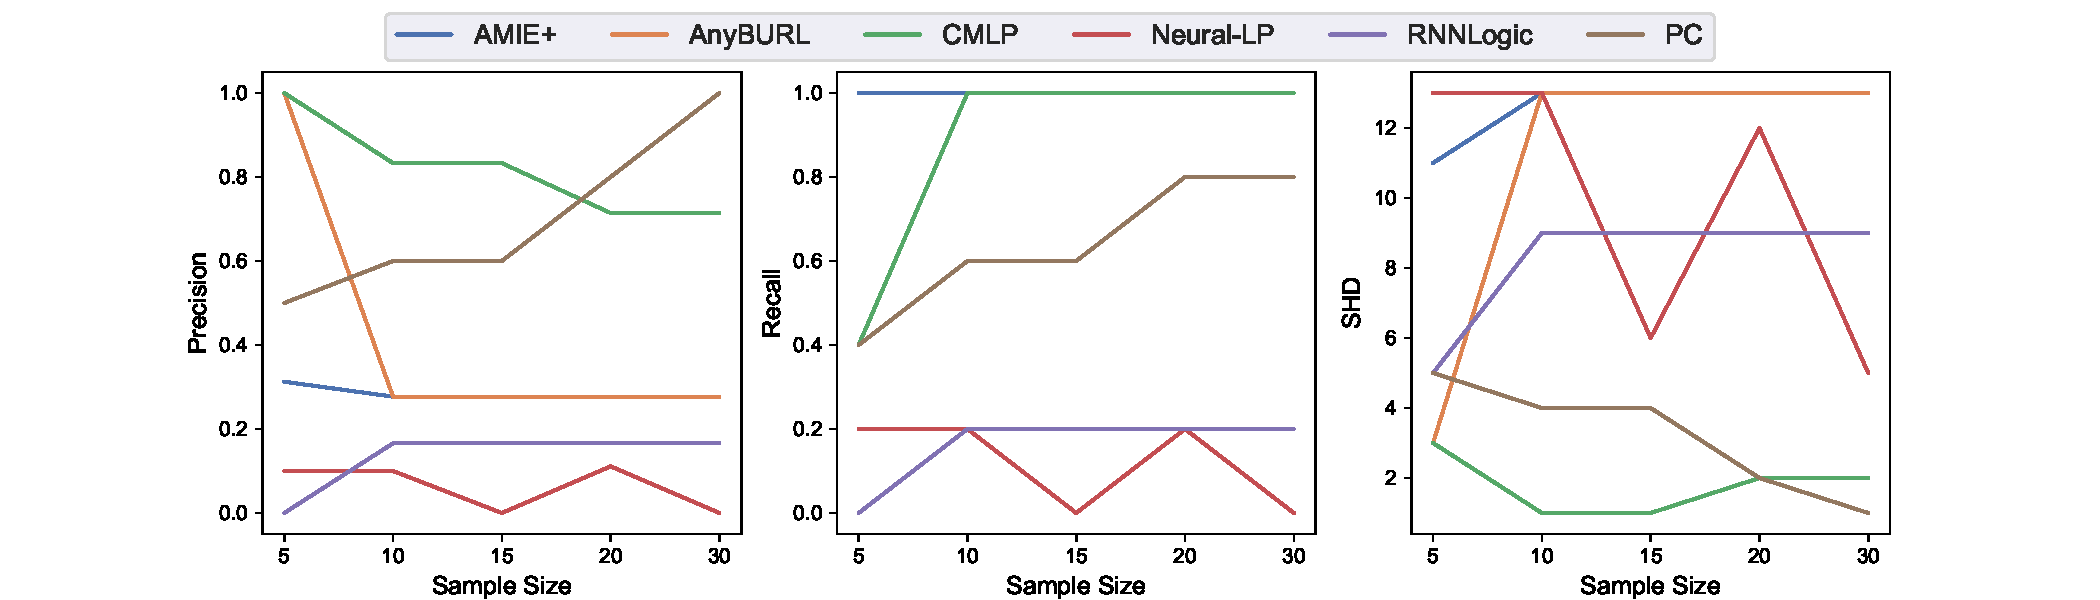
\includegraphics[trim=3cm 0cm 3cm 0cm, width=\linewidth, height=5cm]{figures/allin.pdf}
%     \caption{Precision, recall and SHD results on simulation datasets with differnet sample size. }
%     \label{fig:sim-graph}
% \end{figure*}
\noindent
\textbf{Quality of causal rules from simulations.}
The ground-truth causal graph of KGSs shown in Fig~\ref{fig:simulation}, and
Table~\ref{tab:simulation_rule_quality} shows the accuracy of estimated rules of different methods.
In particular, \dname~ accurately discovers two causal rules in Fig~\ref{fig:simulation} without any redundant rules.
In contrast, correlation-based methods report some non-causal rules.


\begin{table}[t]
\caption{Experimental results on simulation data with $p_{X_1}=0.5$, based on the metrics (precision, recall and SHD), which are commonly used to evaluate the estimated causal graph.}
%\vspace{5pt}
\label{tab:simulation_rule_quality}
\centering
\scalebox{1.2}{
\begin{tabular}{c|c|c|c}
\hline
\textbf{Method} & \textbf{Precision} $\uparrow$ & \textbf{Recall} $\uparrow$ & \textbf{SHD} $\downarrow$ \\
\hline
Neural-LP & 0 & 0& 10 \\
AMIE+ & 0.22 & \textbf{1.0}& 7 \\
RNNLogic & 0.22 & \textbf{1.0}& 7 \\
AnyBURL & 0.25 & \textbf{1.0}& 6 \\
\dname & \textbf{1.0} & \textbf{1.0} & \textbf{0} \\
\hline
\end{tabular}}
\vspace{-4pt}
\end{table}

\begin{table*}[h]
\caption{All rules whose head are $R_3$ and $R_5$, obtained by each algorithm learned on simulated dataset. The strikethroughs indicate the wrong results (there is no entities satisfying the rule).
The rules consistent with the generation process are in bold.
The orange text denotes the weight of each rule with the form max-normalization(original weight)}.

\label{tab:simulation_rule}
\centering
{\tiny
\scalebox{0.75}{
\begin{tabu}{c|l|l|l}
\tabucline[1pt]{-}
\textbf{Method} & \textbf{Rules of $R_3$ with $\mathbf{p_{X_1}=0.5}$} & \textbf{Rules of $R_3$ with $\mathbf{p_{X_1}=0.9}$} & \textbf{Rules of $R_5$}\\
\tabucline[1pt]{-}

\multirow{3}{*}{AMIE+} & \textcolor{orange}{1.00 (0.908)}   $\mathbf{R_3(C_1,C_3) \gets R_1(C_1,C_2), R_2(C_2,C_3)}$  & \textcolor{orange}{1.00 (0.900)}   $\mathbf{R_3(C_1,C_3) \gets R_1(C_1,C_2), R_2(C_2,C_3)}$ & \textcolor{orange}{1.00 (0.898)}   $R_5(C_1,C_3) \gets R_1(C_1,C_2), R_2(C_2,C_3)$\\

& \textcolor{orange}{0.91 (0.829)}   $R_3(C_1,C_3) \gets R_4(C_1,C_3)$ & \textcolor{orange}{0.99 (0.890)}   $R_3(C_1,C_3) \gets R_4(C_1,C_3)$ & \textcolor{orange}{0.99 (0.895)}   $R_5(C_1,C_3) \gets R_3(C_1,C_3)$ \\
&  \textcolor{orange}{0.55 (0.500)}   $R_3(C_1,C_3) \gets R_5(C_1,C_3)$  & \textcolor{orange}{0.91 (0.820)}   $R_3(C_1,C_3) \gets R_5(C_1,C_3)$ & \textcolor{orange}{0.99 (0.894)}   $R_5(C_1,C_3) \gets R_4(C_1,C_3)$\\
\hline
\multirow{3}{*}{AnyBURL}& \textcolor{orange}{1.00 (0.896)} $\mathbf{R_3(C_1,C_3) \gets R_1(C_1,C_2), R_2(C_2,C_3)}$ & \textcolor{orange}{1.00 (0.898)} $R_3(C_1,C_3) \gets R_4(C_1,C_3)$ & \textcolor{orange}{1.00 (0.907)} $R_5(C_1,C_3) \gets R_1(C_1,C_2), R_2(C_2,C_3)$\\
& \textcolor{orange}{0.92 (0.823)} $R_3(C_1,C_3) \gets R_4(C_1,C_3)$ &  \textcolor{orange}{0.99 (0.893)} $\mathbf{R_3(C_1,C_3) \gets R_1(C_1,C_2), R_2(C_2,C_3)}$ & \textcolor{orange}{0.99 (0.902)} $R_5(C_1,C_3) \gets R_3(C_1,C_3)$\\
& \textcolor{orange}{0.56 (0.501)} $R_3(C_1,C_3) \gets R_5(C_1,C_3)$ & \textcolor{orange}{0.91 (0.821)} $R_3(C_1,C_3) \gets R_5(C_1,C_3)$ & \textcolor{orange}{0.99 (0.897)} $R_5(C_1,C_3) \gets R_4(C_1,C_3)$ \\
\hline

\multirow{7}{*}{Neural-LP} & \textcolor{orange}{1.00 (0.318)}  \sout{$R_3(C_1,C_3) \gets R_4(C_1,C_2), R_4(C_2,C_3)$} & \textcolor{orange}{1.00 (0.757)}  \sout{$R_3(C_1,C_3) \gets R_1(C_1,C_2), R_1(C_2,C_3)$}  & \textcolor{orange}{1.00 (0.125)} \sout{$R_5(C_1,C_3) \gets R_4(C_1,C_2),R_3(C_2,C_3)$} \\
& \textcolor{orange}{0.99 (0.316)} \sout{$R_3(C_1,C_3) \gets R_4(C_1,C_2), R_5(C_2,C_3)$} & \textcolor{orange}{0.17 (0.128)} \sout{$R_3(C_1,C_3) \gets R_1(C_1,C_3)$} & \textcolor{orange}{0.78 (0.097)} \sout{$R_5(C_1,C_3) \gets R_3(C_1,C_2),R_3(C_2,C_3)$} \\
& \textcolor{orange}{0.31 (0.100)} \sout{$R_3(C_1,C_3) \gets R_5(C_1,C_2), R_4(C_2,C_3)$} & \textcolor{orange}{0.04 (0.056)} \sout{$R_3(C_1,C_3) \gets R_5(C_2,C_3), R_1(C_1,C_2)$} &\\
& \textcolor{orange}{0.31 (0.099)} \sout{$R_3(C_1,C_3) \gets R_5(C_1,C_2), R_5(C_2,C_3)$} & \textcolor{orange}{0.05 (0.035)} \sout{$R_3(C_1,C_3) \gets R_4(C_2,C_1), R_1(C_3,C_2)$} &\\
& \textcolor{orange}{0.23 (0.073)} $R_3(C_1,C_3) \gets R_4(C_1,C_3)$ & \textcolor{orange}{0.03 (0.025)} $\mathbf{R_3(C_1,C_3) \gets R_1(C_1,C_2), R_2(C_2,C_3)}$\\
& \textcolor{orange}{0.09 (0.028)} \sout{$R_3(C_1,C_3) \gets R_4(C_1,C_2), R_4(C_2,C_3)$} & \\
& \textcolor{orange}{0.07 (0.023)} $R_3(C_1,C_3) \gets R_5(C_1,C_3)$ &\\
\hline

\multirow{3}{*}{RNNLogic} & \textcolor{orange}{1.00 (0.076)}   $\mathbf{R_3(C_1,C_3) \gets R_1(C_1,C_2), R_2(C_2,C_3)}$  & \textcolor{orange}{1.00 (0.071
)}   $\mathbf{R_3(C_1,C_3) \gets R_1(C_1,C_2), R_2(C_2,C_3)}$ & \textcolor{orange}{1.00 (0.220)}   $R_5(C_1,C_3) \gets R_3(C_1,C_3)$\\

& \textcolor{orange}{0.58 (0.044)}   $R_3(C_1,C_3) \gets R_4(C_1,C_3)$ & \textcolor{orange}{0.49 (0.035)}   $R_3(C_1,C_3) \gets R_4(C_1,C_3)$ & \textcolor{orange}{0.28 (0.060)}   $R_5(C_1,C_3) \gets R_4(C_1,C_3)$ \\
&  \textcolor{orange}{0.13 (0.010)}   $R_3(C_1,C_3) \gets R_5(C_1,C_3)$  & \textcolor{orange}{0.14 (0.010)}   $R_3(C_1,C_3) \gets R_5(C_1,C_3)$ & \textcolor{orange}{0.20 (0.045)}   $R_5(C_1,C_3) \gets R_1(C_1,C_2), R_2(C_2,C_3)$\\
\hline


{\dname} & \textcolor{orange}{1.00 (122.797)} $\mathbf{R_3(C_1,C_3) \gets R_1(C_1,C_2), R_2(C_2,C_3)}$ & \textcolor{orange}{1.00 (20.061)} $\mathbf{R_3(C_1,C_3) \gets R_1(C_1,C_2), R_2(C_2,C_3)}$ & -\\

\tabucline[1pt]{-}
\end{tabu}}
}
\end{table*}

\noindent
\textbf{Interpretability of causal rules}
% For rules from the simulation, we analyze all methods' results, whose heads are $R_5$ and $R_6$, and $R_9$ and the results are shown in Table~\ref{tab:simulation_rule} .
% % The rules follow the causal mechanism are in bold.
% There is only one causal rule for $R_5$, which is $R_5(C_1,C_2) \gets R_1(C_1,C_3), R_2(C_3,C_2)$.
% AMIE+, AnyBURL, and \dname~find this causal rule.
% Besides this causal rule, the results of AMIE+ and AnyBURL also include other rules, such as $R_5(C_1,C_2) \gets R_6(C_1,C_2)$ and $R_5(C_1,C_2) \gets R_9(C_1,C_3)$.
% % Especially, for AMIE+ and AnyBURL, note that the weights of $R_3(C_1,C_3) \gets R_4(C_1,C_3)$ are very close to the weights of $R_3(C_1,C_3) \gets R_1(C_1,C_2)$, $ R_2(C_2,C_3)$.
% % It means the algorithms think these two rules have the similar interpretability for the head relation $R_3$.
% % With the change of root node $X_1$'s distribution(from $p_{X_1}=0.5$ to $p_{X_1}=0.9$), AnyBURL even report the higher weight for the rule $R_3(C_1,C_3) \gets R_5(C_1,C_3)$.
% % According to the generation mechanism, the existence of $R_3$ between entities $e_i$ and $e_j$ is independent with whether there is $R_4$ and $R_5$ between $e_i$ and $e_j$.
% % AMIE+ and AnyBURL still return these association rules with high weights, because they only consider whether $R_3$ and $R_4$ co-occur frequently, but not the reason of the co-occurrence.
% The end-to-end deep-model based method(Neural-LP and RNNLogic) fail to discover any correct rules for $R_5$.
Moreover, for the simulation dataset, we analyze all methods' results, whose heads are $R_3$ and $R_5$, and the results are shown in Table~\ref{tab:simulation_rule} (We omit results of $R_4$, since $R_3$ and $R_4$ are symmetric in the causal graph).
The rules follow the causal mechanism are in bold.
There is only one causal rule for $R_3$, which is $R_3(C_1,C_3) \gets R_1(C_1,C_2), R_2(C_2,C_3)$.
AMIE+, AnyBURL, RNNLogic and \dname~find this causal rule.
Besides this causal rule, the results of AMIE+, RNNLogic and AnyBURL also include other rules, such as $R_3(C_1,C_3) \gets R_4(C_1,C_3)$ and $R_3(C_1,C_3) \gets R_5(C_1,C_3)$.
Especially, for those three methods, note that the weights of $R_3(C_1,C_3) \gets R_4(C_1,C_3)$ are very close to the weights of $R_3(C_1,C_3) \gets R_1(C_1,C_2)$, $ R_2(C_2,C_3)$.
It means the algorithms think these two rules have the similar interpretability for the head relation $R_3$.
With the change of root node $X_1$'s distribution(from $p_{X_1}=0.5$ to $p_{X_1}=0.9$), AnyBURL even report the higher weight for the rule $R_3(C_1,C_3) \gets R_5(C_1,C_3)$.
According to the generation mechanism, the existence of $R_3$ between entities $e_i$ and $e_j$ is independent with whether there is $R_4$ and $R_5$ between $e_i$ and $e_j$.
AMIE+, AnyBURL and RNNLogic still return these association rules with high weights, because they only consider whether $R_3$ and $R_4$ co-occur frequently, but not the reason of the co-occurrence.
The end-to-end completion-oriented method, Neural-LP, also return some wrong results, such as the top 1 rule $R_3(C_1,C_3) \gets R_4(C_1,C_2), R_4(C_2,C_3)$, which can not be satisfied by any entities in KG.
The results in~\cite{sadeghian2019drum} show the same phenomenon.
The intermediate results of the completion-oriented method is incomprehensible sometimes.


Furthermore, We sort the rules generated by each algorithm based on their assigned weights and show the five top rules from Douban and Hetionet in Tab.~\ref{tab:rules_recom_result} and Tab.~\ref{tab:rule_hetionet}, respectively.
The results in Tab.~\ref{tab:rules_recom_result} suggests that the ratings for the target movie are highly related to other movies which share the same staff, such as writer, actors, director, etc.
According to the rating results, \dname~ finds a strong causal relationship between the rating of the movie and its editor than other pairs.
The top rules generated by AMIE+ and AnyBURL focus on other shared staffs, but the shared staff has different roles in the target movie and the movie in path.
Those rules of AMIE+ and AnyBURL are hard to be satisfied for most queries.
% By contrast, our mined rules suggest the ratings are determined by the subjective opinions of the users, while the mined rules from other algorithms, including AnyBURL, present the ratings are depended on others related events.
It is worth noting that RNNlogic report the `fan' rules  will impact the users' rating, but \dname~ excludes this kind of rules.
Our results suggest the working ability of the movie's stuff ({\it e.g.} actor or writer) should be the root cause of the users' rate, instead of the followers of the stuff.
From the rules from Hetionet, we can see
% Similar to the results on simulation dataset,
the learned rules are broadly divided into two classes, those in which the target drug and disease are connected by therapeutic information about the similar disease and drug, and those in which the target drug and disease are connected by commonly associated genes.
Further, we find that the rules mined by AnyBURL also contain rules for reasoning through shared side effects.



% Logically incorrect rules are highlighted by italic-red. This experiment shows two of the three top ranked rules generated by Neural LP are incorrect (for both head predicates wif e and son
\begin{table*}[t]
\centering
\caption{Top 5 Rules to infer HighRate(User, Movie) given by the methods. The strikethroughs indicate the wrong results (there is no entities satisfying the rule).
}
\label{tab:rules_recom_result}
\vspace{-1pt}
{\tiny
\begin{tabular}{c|l}
\hline
\textbf{Method} & \multicolumn{1}{c}{\textbf{ Top rules to infer HighRate(User, Movie)}} \\
\hline

\multirow{5}{*}{AMIE+} &
\textcolor{orange}{1.00 (0.565)} HighRate(User,Movie) $\gets$ HighRate(User,Movie1), Writer(Person,Movie1),Director(Person,Movie)\\
& \textcolor{orange}{0.98 (0.556)} HighRate(User,Movie) $\gets$ HighRate(User,Movie1), Director(Person,Movie1), Writer(Person,Movie)\\
& \textcolor{orange}{0.87 (0.489)} HighRate(User,Movie) $\gets$ HighRate(User,Movie1), Writer(Person,Movie1), Actress(Person,Movie)\\
& \textcolor{orange}{0.74 (0.417)} HighRate(User,Movie) $\gets$ HighRate(User,Movie1), Director(Person,Movie1), Actor(Person,Movie)\\
& \textcolor{orange}{0.72 (0.405)} HighRate(User,Movie) $\gets$ HighRate(User,Movie1), Actress(Person,Movie1), Writer(Person,Movie)\\
\hline

\multirow{5}{*}{AnyBURL} &
\textcolor{orange}{1.00 (0.400)} HighRate(User,Movie) $\gets$ HighRate(User,Movie1), Composer(Person,Movie1), Actor(Person,Movie)\\
& \textcolor{orange}{0.99(0.397)} HighRate(User,Movie) $\gets$ HighRate(User,Movie1), Producer(Person,Movie1), Director(Person,Movie)\\
& \textcolor{orange}{0.97 (0.386)} HighRate(User,Movie) $\gets$ HighRate(User,Movie1), Director(Person,Movie1), Actress(Person,Movie)\\
& \textcolor{orange}{0.89 (0.355)} HighRate(User,Movie) $\gets$ HighRate(User,Movie1), Writer(Person,Movie1), Actress(Person,Movie)\\
& \textcolor{orange}{0.85 (0.340)} HighRate(User,Movie) $\gets$ HighRate(User,Movie1), Editor(Person,Movie1), Editor(Person,Movie)\\
\hline



\multirow{2}{*}{Neural-LP}
& \textcolor{orange}{1.00 (0.120)} HighRate(User,Movie) $\gets$ HighRate(User,Movie1), HighRate(User1,Movie1), HighRate(User1,Movie)\\
& \textcolor{orange}{0.28 (0.034)} HighRate(User,Movie) $\gets$ HighRate(User,Movie1), MovieType(Movie1,Type), MovieType(Movie,Type)\\
\hline


\multirow{5}{*}{RNNLogic} &
\textcolor{orange}{1.00 (0.011)} HighRate(User,Movie) $\gets$ Fan(User,Person),Editor(Person,Movie)\\
&\textcolor{orange}{0.45 (0.005)} HighRate(User,Movie) $\gets$ Fan(User,Person),Actor(Person,Movie)\\
&\textcolor{orange}{0.36 (0.004)} HighRate(User,Movie) $\gets$ Fan(User,Person),Director(Person,Movie)\\
&\textcolor{orange}{0.36 (0.004)} HighRate(User,Movie) $\gets$ Fan(User,Person),Writer(Person,Movie)\\
&\textcolor{orange}{0.36 (0.004)} HighRate(User,Movie) $\gets$ Fan(User,Person),Composer(Person,Movie)\\
\hline

\multirow{5}{*}{\dname} &
\textcolor{orange}{1.00 (0.034)} HighRate(User,Movie) $\gets$ HighRate(User,Movie1), Editor(Person,Movie1), Editor(Person,Movie)\\

& \textcolor{orange}{0.12 (0.004)} HighRate(User,Movie1) $\gets$ HighRate(User,Movie1),Cinematographer(Person,Movie),Cinematographer(Person,Movie)
\\
& \textcolor{orange}{0.06 (0.002)} HighRate(User,Movie1) $\gets$ HighRate(User,Movie1),Writer(Person,Movie),Writer(Person,Movie)\\
& \textcolor{orange}{0.06 (0.002)} HighRate(User,Movie1) $\gets$ HighRate(User,Movie1),Actress(Person,Movie),Actress(Person,Movie)\\
& \textcolor{orange}{0.03 (0.001)} HighRate(User,Movie1) $\gets$ HighRate(User,Movie1),Director(Person,Movie),Actor(Person,Movie)\\
\hline
\end{tabular}
}
\end{table*}


\begin{table*}
\centering
\caption{Top 5 Rules to infer Treats(Compound, Disease) given by the methods. For brevity, we use `C' and `D' for compound and disease, respectively.}
\label{tab:rule_hetionet}
{\tiny
\begin{tabular}{c|l}
    \hline
    \textbf{Method} & \multicolumn{1}{c}{\textbf{ Top rules to infer Treats(Compound, Disease)}} \\ \hline
    \multirow{5}{*}{AMIE+} &
\textcolor{orange}{1.00 (0.393)}
Treats(C, D) $\gets$ Resembles(C,C1), Treats(C1, D)
    \\
& \textcolor{orange}{0.82 (0.322)}
Treats(C, D) $\gets$ Resembles(C1,C),Treats(C1, D)
\\
& \textcolor{orange}{0.42 (0.167)} Treats(C, D) $\gets$ Downregulates(C,Gene1), Associates(D,Gene1)
\\
& \textcolor{orange}{0.38 (0.151)} Treats(C, D) $\gets$ Downregulates(C,Gene1), Upregulates(D,Gene1)
 \\
& \textcolor{orange}{0.37 (0.144)} Treats(C, D) $\gets$ Binds(C,Gene1), Upregulates(D,Gene1)
\\


\hline
\multirow{5}{*}{AnyBURL} & \textcolor{orange}{1.00 (0.319)}
Treats(C, D) $\gets$ Includes(PharmacologicClass1,C),Includes(PharmacologicClass1,C1),Treats(C1, D)
 \\
& \textcolor{orange}{0.60 (0.192)}
Treats(C, D) $\gets$ Resembles(C1,C),Treats(C1, D)
 \\
& \textcolor{orange}{0.52 (0.166)}
Treats(C, D) $\gets$ Resembles(C1,C),Resembles(C1,C2),Treats(C2, D)
 \\
& \textcolor{orange}{0.31 (0.098)}
Treats(C, D) $\gets$ Resembles(C1,C),Resembles(C2,C1),Treats(C2, D)
 \\
& \textcolor{orange}{0.24 (0.077)}
Treats(C, D) $\gets$ Treats(C, D1), Resembles(D1,D)
 \\ \hline


\multirow{1}{*}{Neural-LP} &
\textcolor{orange}{1.00 (0.659)}
Treats(C, D) $\gets$ Treats(C, D1), Treats(C1, D1),Treats(C1, D)
\\ \hline



\multirow{2}{*}{RNNLogic} &
\textcolor{orange}{1.00 (0.00007)}
Treats(C, D) $\gets$ Resembles(C, C1),Treats(C1, D)
 \\
& \textcolor{orange}{1.00 (0.00007)}

Treats(C, D) $\gets$ Resembles(C, C1),
Resembles(C1, C2),Treats(C2, D)
\\ \hline


\multirow{5}{*}{\dname} &
\textcolor{orange}{1.00 (269.00))}
Treats(C, D) $\gets$ Treats(C, D1),Resembles(D1, D2),Resembles(D, D2)
 \\
    & \textcolor{orange}{0.85 (229.32))}
Treats(C, D) $\gets$ Includes(PharmacologicClass1, C),Includes(PharmacologicClass1, C1),Treats(C1, D)

\\
    & \textcolor{orange}{0.83 (224.37))}
Treats(C, D) $\gets$
Treats(C, D1),Resembles(D2, D1),Resembles(D2, D)
\\
    & \textcolor{orange}{0.58 (155.18))}
Treats(C, D) $\gets$ Treats(C, D1),Treats(C1, D1),Treats(C1, D)


\\
    & \textcolor{orange}{0.10 (26.52))}
 Treats(C, D) $\gets$
 Treats(C, D1),
 Resembles(D2,D1),
 Resembles(D,D1)

    \\ \hline

\end{tabular}
}
\end{table*}


% \begin{table*}
% \caption{Top Rules to infer $User\stackrel{Rate}{\longrightarrow}Movie$ given by the methods.}
% \label{tab:rule_douban}
% \begin{tabular}{c|l}
%     \hline
%     \textbf{Method} & \multicolumn{1}{c}{\textbf{ Top rules to infer $User\stackrel{Rate}{\longrightarrow}Movie$}} \\ \hline
%     \multirow{3}{*}{AMIE+} &
%     1. $User\stackrel{Fan}{\longrightarrow}Person\stackrel{Director}{\longrightarrow}Movie$ \\
%     & 2. $User\stackrel{Fan}{\longrightarrow}Person\stackrel{Writer}{\longrightarrow}Movie$ \\
%     & 3. $User\stackrel{Rate}{\longrightarrow}Movie1\stackrel{Director}{\longleftarrow}Person\stackrel{Director}{\longrightarrow}Movie$ \\ \hline
%     \multirow{3}{*}{AnyBURL} &  1. $User\stackrel{Rate}{\longrightarrow}Movie1\stackrel{Wish}{\longleftarrow}User1\stackrel{Rate}{\longrightarrow}Movie$ \\
%     & 2. $User\stackrel{Rate}{\longrightarrow}Movie1\stackrel{Director}{\longleftarrow}Person\stackrel{Actor}{\longrightarrow}Movie$ \\
%     & 3. $User\stackrel{Rate}{\longrightarrow}Movie1\stackrel{Producer}{\longleftarrow}Person\stackrel{Actor}{\longrightarrow}Movie$ \\ \hline
%     \multirow{3}{*}{Neural-LP} & 1. $User\stackrel{Rate}{\longrightarrow}Movie1\stackrel{Rate}{\longleftarrow}User1\stackrel{Rate}{\longrightarrow}Movie$ \\
%     & 2. $User\stackrel{Rate}{\longrightarrow}Movie1\stackrel{titleType}{\longleftarrow}MovieType\stackrel{titleType}{\longrightarrow}Movie$ \\
%     & 3. $User\stackrel{Wish}{\longrightarrow}Movie1\stackrel{archivesound}{\longleftarrow}Person\stackrel{archivesound}{\longrightarrow}Movie$ \\ \hline
%     \multirow{3}{*}{RNNLogic} & 1. $User\stackrel{Fan}{\longrightarrow}Person\stackrel{Actor}{\longrightarrow}Movie$ \\
%     & 2. $User\stackrel{Fan}{\longrightarrow}Person\stackrel{Director}{\longrightarrow}Movie$ \\
%     & 3. $User\stackrel{Fan}{\longrightarrow}Person\stackrel{Writer}{\longrightarrow}Movie$ \\ \hline
%     \multirow{3}{*}{\dname} & 1. $User\stackrel{Rate}{\longrightarrow}Movie1\stackrel{Writer}{\longleftarrow}Person\stackrel{Writer}{\longrightarrow}Movie$ \\
%     & 2. $User\stackrel{Rate}{\longrightarrow}Movie1\stackrel{Actress}{\longleftarrow}Person\stackrel{Actress}{\longrightarrow}Movie$ \\
%     & 3.$User\stackrel{Rate}{\longrightarrow}Movie1\stackrel{Director}{\longleftarrow}Person\stackrel{Actor}{\longrightarrow}Movie$ \\ \hline
% \end{tabular}
% \end{table*}

% \begin{table*}[t]
% \centering
% \caption{Top 3 Rules of HighRate given by the methods.The strikethroughs indicate the wrong results (there is no entities satisfying the rule).
% The orange text denotes the weight of each rule with the form max-normalization(original weight)}
% \label{tab:rules_recom_result}
% \vspace{-1pt}
% \begin{tabular}{c|l}
% \hline
% \textbf{Method} & \multicolumn{1}{c}{\textbf{Rules of HighRate}} \\
% \hline
% \multirow{3}{*}{Neural-LP} &
% \textcolor{orange}{1.00 (0.636)} \sout{HighRate(User,Movie) $\gets$ Saw(User1,Movie), Saw(User2,User1)}\\
%  &    \textcolor{orange}{0.50 (0.320)} \sout{HighRate(User,Movie) $\gets$ Saw(User1,Movie), Saw(User2,User1),Saw(User,User2)} \\
%   &  \textcolor{orange}{0.02(0.011)}  HighRate(User,Movie) $\gets$ Saw(User, Movie)\\
% \hline
% \multirow{3}{*}{AMIE+} &
% \textcolor{orange}{1.00 (0.662)} HighRate(User,Movie) $\gets$ Fan(User, Person), Director(Person,Movie) \\
% & \textcolor{orange}{0.99 (0.658)} HighRate(User,Movie) $\gets$ Fan(User, Person), Writer(Person,Movie) \\
% & \textcolor{orange}{0.85 (0.565)} HighRate(User,Movie) $\gets$ HighRate(User,Movie1), Writer(Person,Movie1),Director(Person,Movie)\\
% \hline
% \multirow{5}{*}{AnyBURL} &
% \textcolor{orange}{1.00 (0.286)} HighRate(User,Movie) $\gets$ HighRate(User,Movie1), Wish(User1,Movie1),HighRate(User1,Movie) \\
% & \textcolor{orange}{0.97 (0.276)} HighRate(User,Movie) $\gets$ HighRate(User,Movie1), Director(Person,Movie1),Actor(Person,Movie)
% \\
% & \textcolor{orange}{0.97 (0.276)} HighRate(User,Movie) $\gets$ HighRate(User,Movie1), Producer(Person,Movie1),Actor(Person,Movie)\\
% & $\dots$ \\
% & \textcolor{orange}{0.983 (0.236)} HighRate(User,Movie) $\gets$ Fan(User,Person), Director(Person,Movie) \\
% \hline
% \multirow{3}{*}{RNNLogic} &
% \textcolor{orange}{1.00 (0.0048)} HighRate(User,Movie) $\gets$ Fan(User,Person), Actor(Person,Movie) \\
% & \textcolor{orange}{0.875 (0.0042)} HighRate(User,Movie) $\gets$ Fan(User,Person), Director(Person,Movie) \\
% & \textcolor{orange}{0.85 (0.0041)} HighRate(User,Movie) $\gets$ Fan(User,Person), Writer(Person,Movie) \\

% \hline
% \multirow{3}{*}{\dname} &
% \textcolor{orange}{1.00 (0.035)} HighRate(User,Movie) $\gets$ HighRate(User,Movie1),Writer(Person,Movie1),Writer(Person,Movie) \\
% & \textcolor{orange}{0.06 (0.002)} HighRate(User,Movie1) $\gets$ HighRate(User,Movie1),Actress(Person,Movie),Actress(Person,Movie)
% \\
% & \textcolor{orange}{0.06 (0.002)} HighRate(User,Movie1) $\gets$ HighRate(User,Movie1),Director(Person,Movie),Actor(Person,Movie)\\
% \hline
% \end{tabular}
% \end{table*}

% We conducted an experimental study in which we investigated the performance of the learned causal rules in two aspects: the explainability to the KG and the usefulness for downstream task, such as link prediction.
% Our main goal is to provide insight into
% \begin{itemize}
%     \item the explainability of the learned causal rules to the KG.
%     \item the effectiveness of the learned causal rules or downstream task, such as link prediction.
%     \item the empirical conclusions for the hyper-parameters and alternative algorithms in our framework.
% \end{itemize}
% Furthermore, we briefly summarize the experiment designs to achieve the above-mentioned the goal under the available resources.

% Goal 1 	$\Rightarrow$ We use the simulation KG to quantitatively evaluate the learned causal rules from KG, since the causal relationships are inaccessible for real dataset\footnote{This is the most commonly used way for the evaluation of the causal discovery methods in both relational and propositional data\cite{zheng2018dags, lee2016learning}}.
% Meanwhile, the case study for real data will be introduced to qualitatively discuss the quality of mined rules.

% Goal 2 	$\Rightarrow$ 
%!TEX root = ../main.tex
\section{Related Works}
\label{sec:related}

\stitle{Retrieval Augmented Generation Question Answering.}
%
Large languaga models sometimes generate factually incorrect or misleading information, often due to a lack of real-time knowledge or limited access to external facts beyond their training data.
RAG-based Question Answering addresses this by integrating external knowledge retrieval into the generation process. By retrieving relevant document chunks through semantic search, RAG ensures that the model’s responses are grounded in accurate, real-world information, effectively reducing the likelihood of hallucinations.
Early approaches focused on jointly training the retriever and generator, ensuring that the retrieved content aligned with the generation model’s intent to provide more accurate answers~\cite{izacard2023atlas}. With the success of in-context learning, more recent work has treated the retriever as a separate module, directly providing retrieved information to the model via prompts~\cite{wang2023knowledgptenhancinglargelanguage}.
As retrieval technologies have advanced, RAG-based systems now support multimodal retrieval, enabling answers that draw from diverse data sources~\cite{chen2021open, chen-etal-2022-murag, luo-etal-2023-unifying}. 
%For example, OTT-QA~\cite{chen2021open}  retrieves both tables and text, MuRAG~\cite{chen-etal-2022-murag} integrates text and images, and MMQA~\cite{luo-etal-2023-unifying} combines text, tables, and images to handle complex queries.
% \yang{It's hard for us to compare Symphony with existing systems.}


\stitle{Trustworthiness of Large Language Models.}
%
The trustworthiness of LLMs is essential for their effective deployment in real-world applications. To assess LLM trustworthiness, researchers have proposed various approaches. For example, TrustLLM~\cite{huang2024trustllmtrustworthinesslargelanguage} provides a comprehensive framework for evaluating LLMs across different trust dimensions.
However, evaluating LLM trustworthiness remains challenging, with gaps in holistic assessment approaches. Some studies suggest that self-evaluation, where LLMs assess their confidence in the generated outputs, can help improve selective generation and mitigate inaccuracies~\cite{Ren2023SelfEvaluationIS}. Additionally, understanding the internal mechanisms of LLMs, such as the use of local intrinsic dimension (LID) for predicting truthfulness, has been proposed as a way to measure model reliability~\cite{Yin2024CharacterizingTI}.
In our work, we aim to improve the trustworthiness of LLMs through post-verification, ensuring that generated outputs are validated against reliable sources after generation to minimize inaccuracies and enhance their overall reliability.
\section{Concluding Remarks}
\label{sec:discussion}
In this paper, we reconcile efficiency and security for uplink communication in Federated Learning. 
We propose to adapt existing compression mechanisms such as scalar quantization and pruning to the secure aggregation protocol by imposing a linearity constraint on the decompression operator. 
Our experiments demonstrate that we can adapt both quantization and pruning mechanisms to obtain a high degree of uplink compression with minimal degradation in performance and higher security guarantees. For achieving the highest rates of compression, we introduce \SecInd, a variant of \SecAgg well-suited for TEE-based implementation that supports product quantization while maintaining a high security bar. 
%We plan to extend our work to other federated learning scenarios, such as asynchronous FL, and further investigate the interaction of compression and privacy.
%\section{Extensions} 
As mentioned in Section~\ref{sec:intro}, we {may want } both \SecAgg and Differential Privacy~\citep{abadi2016deep} to realize the full promise of FL as a privacy-enhancing technology. 
While our primary focus is on enabling efficient and secure uplink communication, we emphasize that the proposed approaches are compatible with user-level DP. 
For instance, {at the cost of increasing the complexity of the trusted computing base}, DP noise can be added natively by the TEE with our modified random pruning or scalar quantization approaches. 
For PQ  and \SecInd, {we can have the TEE to add noise in the assignment space (\ie outputting a noisy histogram), or to map the histogram to the codeword space and add noise there.
Each option offers a different tradeoff between privacy, trust, and accuracy; we leave detailed evaluation to future work.}




%\modif{\textbf{Compatibility with DP.} 
%\sout{it would require, however, to transfer the aggregation to TEE or to design a DP mechanism in the assignment space, since DP noise must be added by the TEE and not by the server.}}

%\modif{\textbf{Efficiency and Privacy.}} A separate line of work {aims} to combine communication efficiency and privacy. 
%For instance, \cite{triastcyn2021dprec} develop a method that unifies compressed communication and DP (where integration with \SecAgg is left as an open problem), while \cite{chaudhuri2022privacyaware} design a privacy-aware scalar compression mechanism within the \emph{local} differential privacy model.

%\graham{\sout{
%\modif{\textbf{Broader Social Impact. }} In this work, we propose to enhance the privacy of individuals who may contribute to training ML models and simultaneously enable more individuals to participate in private training, who might otherwise have been excluded due to resource constraints. }}
% Indeed, Federated Learning could enable a malicious server to access individual model updates that can leak personal information. Hence, we propose a secure way to communicate the individual model updates.

% - Generic and less data-dependent codebook
% - Model compression 
% - Compression and DP
% - Error correction

% There are multiple extensions of PQ, such as having multiple codebooks per matrix  (which increases the cost of storing the codebooks) or performing the assignments with other norms than the $L_2$ norm.



% As a side note, \cite{jia2022federated} propose to perform domain adaptation by fine-tuning a small fraction of the model parameters, which is naturally compatible with Secure Aggregation, but requires to start from a pretrained model. 





%%
%% The next two lines define the bibliography style to be used, and
%% the bibliography file.

\begin{thebibliography}{10}

\bibitem{Bonawitz2017PracticalSA}
K.~Bonawitz, V.~Ivanov, B.~Kreuter, A.~Marcedone, H.~McMahan, S.~Patel,
  D.~Ramage, A.~Segal, and K.~Seth.
\newblock Practical secure aggregation for privacy-preserving machine learning.
\newblock {\em CCS}, 2017.

\bibitem{chai2020secure}
D.~Chai, L.~Wang, K.~Chen, and Q.~Yang.
\newblock Secure federated matrix factorization.
\newblock {\em IEEE Intelligent Systems}, 2020.

\bibitem{ganti2011mobile}
R.~K. Ganti, F.~Ye, and H.~Lei.
\newblock Mobile crowdsensing: current state and future challenges.
\newblock {\em IEEE Communications Magazine}, 49(11):32--39, 2011.

\bibitem{han2021hidden}
X.~Han, L.~Wang, and W.~Fan.
\newblock Is hidden safe? location protection against machine-learning
  prediction attacks in social networks.
\newblock {\em MIS Quarterly}, 45(2):821--858, 2021.

\bibitem{konevcny2016federated}
J.~Kone{\v{c}}n{\`y}, H.~B. McMahan, F.~X. Yu, P.~Richt{\'a}rik, A.~T. Suresh,
  and D.~Bacon.
\newblock Federated learning: Strategies for improving communication
  efficiency.
\newblock {\em arXiv:1610.05492}, 2016.

\bibitem{li2014the}
H.~{Li}, B.~{Zhao}, and A.~{Fuxman}.
\newblock The wisdom of minority: discovering and targeting the right group of
  workers for crowdsourcing.
\newblock In {\em WWW}, pages 165--176, 2014.

\bibitem{li2016survey}
Y.~Li, J.~Gao, C.~Meng, Q.~Li, L.~Su, B.~Zhao, W.~Fan, and J.~Han.
\newblock A survey on truth discovery.
\newblock {\em SIGKDD Explor. Newsl.}, 17(2):1–16, Feb. 2016.

\bibitem{Li2018AnET}
Y.~Li, C.~Miao, L.~Su, J.~Gao, Q.~Li, B.~Ding, Z.~Qin, and K.~Ren.
\newblock An efficient two-layer mechanism for privacy-preserving truth
  discovery.
\newblock {\em KDD}, 2018.

\bibitem{Li2020TowardsDP}
Y.~Li, H.~Xiao, Z.~Qin, C.~Miao, L.~Su, J.~Gao, K.~Ren, and B.~Ding.
\newblock Towards differentially private truth discovery for crowd sensing
  systems.
\newblock {\em ICDCS}, pages 1156--1166, 2020.

\bibitem{liu2020secure}
Y.~{Liu}, Y.~{Kang}, C.~{Xing}, T.~{Chen}, and Q.~{Yang}.
\newblock A secure federated transfer learning framework.
\newblock {\em IEEE Intelligent Systems}, 35(4):70--82, 2020.

\bibitem{ma2014opportunities}
H.~Ma, D.~Zhao, and P.~Yuan.
\newblock Opportunities in mobile crowd sensing.
\newblock {\em IEEE Communications Magazine}, 52(8):29--35, 2014.

\bibitem{meng2015truth}
C.~Meng, W.~Jiang, Y.~Li, J.~Gao, L.~Su, H.~Ding, and Y.~Cheng.
\newblock Truth discovery on crowd sensing of correlated entities.
\newblock In {\em Proceedings of the 13th ACM Conference on Embedded Networked
  Sensor Systems}, pages 169--182, 2015.

\bibitem{Miao2015CloudEnabledPT}
C.~Miao, W.~Jiang, L.~Su, Y.~Li, S.~Guo, Z.~Qin, H.~Xiao, J.~Gao, and K.~Ren.
\newblock Cloud-enabled privacy-preserving truth discovery in crowd sensing
  systems.
\newblock In {\em SenSys}, 2015.

\bibitem{Miao2019PrivacyPreservingTD}
C.~Miao, W.~Jiang, L.~Su, Y.~Li, S.~Guo, Z.~Qin, H.~Xiao, J.~Gao, and K.~Ren.
\newblock Privacy-preserving truth discovery in crowd sensing systems.
\newblock {\em ACM Transactions on Sensor Networks}, 15:1 -- 32, 2019.

\bibitem{Miao2017ALP}
C.~Miao, L.~Su, W.~Jiang, Y.~Li, and M.~Tian.
\newblock A lightweight privacy-preserving truth discovery framework for mobile
  crowd sensing systems.
\newblock {\em INFOCOM}, pages 1--9, 2017.

\bibitem{ouyang2015truth}
R.~W. Ouyang, M.~Srivastava, A.~Toniolo, and T.~J. Norman.
\newblock Truth discovery in crowdsourced detection of spatial events.
\newblock {\em IEEE transactions on knowledge and data engineering},
  28(4):1047--1060, 2015.

\bibitem{Peng2018DataQG}
D.~Peng, F.~Wu, and G.~Chen.
\newblock Data quality guided incentive mechanism design for crowdsensing.
\newblock {\em IEEE Transactions on Mobile Computing}, 17:307--319, 2018.

\bibitem{epflmobility}
M.~Piorkowski, N.~Sarafijanovic-Djukic, and M.~Grossglauser.
\newblock {CRAWDAD} dataset epfl/mobility (v. 2009-02-24).
\newblock Downloaded from \url{https://crawdad.org/epfl/mobility/20090224},
  Feb. 2009.

\bibitem{Primault2019TheLR}
V.~Primault, A.~Boutet, S.~B. Mokhtar, and L.~Brunie.
\newblock The long road to computational location privacy: A survey.
\newblock {\em IEEE Communications Surveys \& Tutorials}, 21:2772--2793, 2019.

\bibitem{Reddy2010ExaminingMF}
S.~Reddy, D.~Estrin, M.~Hansen, and M.~Srivastava.
\newblock Examining micro-payments for participatory sensing data collections.
\newblock {\em UbiComp}, 2010.

\bibitem{shamir1979share}
A.~Shamir.
\newblock How to share a secret.
\newblock {\em Communications of the ACM}, 22(11):612--613, 1979.

\bibitem{tang2011secure}
C.~Tang, G.~Shi, and Z.~Yao.
\newblock Secure multi-party computation protocol for sequencing problem.
\newblock {\em SCIENTIA SINICA Informationis}, 41(7):789--797, 2011.

\bibitem{Tang2018NonInteractivePT}
X.~Tang, C.~Wang, X.~Yuan, and Q.~Wang.
\newblock Non-interactive privacy-preserving truth discovery in crowd sensing
  applications.
\newblock {\em INFOCOM}, pages 1988--1996, 2018.

\bibitem{Wang2014SurrogateMS}
D.~Wang, T.~Abdelzaher, and L.~M. Kaplan.
\newblock Surrogate mobile sensing.
\newblock {\em IEEE Communications Magazine}, 52:36--41, 2014.

\bibitem{wang2013credibility}
D.~Wang, L.~Kaplan, T.~Abdelzaher, and C.~C. Aggarwal.
\newblock On credibility estimation tradeoffs in assured social sensing.
\newblock {\em IEEE Journal on Selected Areas in Communications},
  31(6):1026--1037, 2013.

\bibitem{wang2012truth}
D.~Wang, L.~Kaplan, H.~Le, and T.~Abdelzaher.
\newblock On truth discovery in social sensing: A maximum likelihood estimation
  approach.
\newblock In {\em IPSN}, pages 233--244, 2012.

\bibitem{Wang2017LocationPT}
L.~Wang, D.~Yang, X.~Han, T.~Wang, D.~Zhang, and X.~Ma.
\newblock Location privacy-preserving task allocation for mobile crowdsensing
  with differential geo-obfuscation.
\newblock {\em WWW}, 2017.

\bibitem{Wang2019MobileCT}
L.~Wang, D.~Yang, X.~Han, D.~Zhang, and X.~Ma.
\newblock Mobile crowdsourcing task allocation with differential-and-distortion
  geo-obfuscation.
\newblock {\em IEEE Transactions on Dependable and Secure Computing},
  18:967--981, 2021.

\bibitem{Wang2020SparseMC}
L.~Wang, D.~Zhang, D.~Yang, B.~Y. Lim, X.~Han, and X.~Ma.
\newblock Sparse mobile crowdsensing with differential and distortion location
  privacy.
\newblock {\em IEEE Transactions on Information Forensics and Security},
  15:2735--2749, 2020.

\bibitem{wang2016differential}
L.~Wang, D.~Zhang, D.~Yang, B.~Y. Lim, and X.~Ma.
\newblock Differential location privacy for sparse mobile crowdsensing.
\newblock In {\em ICDM}, pages 1257--1262. IEEE, 2016.

\bibitem{Wang2021AST}
T.~Wang, C.~Lv, C.~Wang, F.~Chen, and Y.~Luo.
\newblock A secure truth discovery for data aggregation in mobile crowd
  sensing.
\newblock {\em Secur. Commun. Networks}, 2021:2296386:1--2296386:15, 2021.

\bibitem{Wang2019PersonalizedPT}
Z.~Wang, J.~Hu, R.~Lv, J.~Wei, Q.~Wang, D.~Yang, and H.~Qi.
\newblock Personalized privacy-preserving task allocation for mobile
  crowdsensing.
\newblock {\em IEEE Transactions on Mobile Computing}, 18:1330--1341, 2019.

\bibitem{Whitehill2009WhoseVS}
J.~Whitehill, P.~Ruvolo, T.~Wu, J.~Bergsma, and J.~Movellan.
\newblock Whose vote should count more: Optimal integration of labels from
  labelers of unknown expertise.
\newblock In {\em NeurIPS}, 2009.

\bibitem{Xu2019EfficientAP}
G.~Xu, H.~Li, S.~Liu, M.~Wen, and R.~Lu.
\newblock Efficient and privacy-preserving truth discovery in mobile crowd
  sensing systems.
\newblock {\em IEEE Transactions on Vehicular Technology}, 68:3854--3865, 2019.

\bibitem{yang2019federated}
Q.~Yang, Y.~Liu, T.~Chen, and Y.~Tong.
\newblock Federated machine learning: Concept and applications.
\newblock {\em ACM Transactions on Intelligent Systems and Technology},
  10(2):12, 2019.

\bibitem{yin2008truth}
X.~Yin, J.~Han, and S.~Y. Philip.
\newblock Truth discovery with multiple conflicting information providers on
  the web.
\newblock {\em IEEE Transactions on Knowledge and Data Engineering},
  20(6):796--808, 2008.

\bibitem{ZHANG2020101848}
C.~Zhang, C.~Xu, L.~Zhu, Y.~Li, C.~Zhang, and H.~Wu.
\newblock An efficient and privacy-preserving truth discovery scheme in
  crowdsensing applications.
\newblock {\em Computers \& Security}, 97:101848, 2020.

\bibitem{Zhang2021ReliableAP}
C.~Zhang, L.~Zhu, C.~Xu, X.~Liu, and K.~Sharif.
\newblock Reliable and privacy-preserving truth discovery for mobile
  crowdsensing systems.
\newblock {\em IEEE Transactions on Dependable and Secure Computing},
  18:1245--1260, 2021.

\bibitem{zhang20144w1h}
D.~Zhang, L.~Wang, H.~Xiong, and B.~Guo.
\newblock 4w1h in mobile crowd sensing.
\newblock {\em IEEE Communications Magazine}, 52(8):42--48, 2014.

\bibitem{Zheng2018LearningTT}
Y.~Zheng, H.~Duan, and C.~Wang.
\newblock Learning the truth privately and confidently: Encrypted
  confidence-aware truth discovery in mobile crowdsensing.
\newblock {\em IEEE Transactions on Information Forensics and Security},
  13:2475--2489, 2018.

\bibitem{Zheng2020PrivacyAwareAE}
Y.~Zheng, H.~Duan, X.~Yuan, and C.~Wang.
\newblock Privacy-aware and efficient mobile crowdsensing with truth discovery.
\newblock {\em IEEE Transactions on Dependable and Secure Computing},
  17:121--133, 2020.

\end{thebibliography}



\appendix

\section{Datasets for FEL}
\label{sec:datasets}
In this section we would like to provide more details about our experiments. We first provide details about each dataset that was used. We then provide details about the model architectures that we used for each dataset.  


\subsection{Production Dataset}
Production dataset is an internal dataset that captures whether a user installs a mobile application after being shown a relevant advertisement item. A few hundred features are used as an input (the exact number cannot be disclosed) to predict a binary label (install/not-install). All the input features are public. For training, we use advertisement data from a random sample of 35 million users over a period of one month. Randomly selected 15 million users from the following week were used for testing.  

%\subsection{Open-Source Datasets}

\subsection{Taobao CTR Dataset}
The Taobao dataset contains 26 million interactions (click/non-click when an Ad was shown) between 1.14 million users and 847 thousand items across an 8-day period. 
The dataset uses 9 user features (e.g., gender or occupation), 6 item features (e.g., price or brand), and two contextual features (e.g., the day of week), which we assume to be all public to the service provider. 

In the Taobao CTR dataset, 16 out of the 17 features are sparse, with a categorical value encoding instead of a continuous, floating point value.
%
While server-based recommendation models use large embedding tables to convert these sparse features into a floating point embedding~\cite{din, dlrm, wideanddeep}, training such embedding tables on device is complicated because of the large memory capacity requirement (e.g., in the order of GB to TB~\cite{zhao2020distributed,acun:2021:understandingtraining,wilkening:2021:recssd,lui:2021:capacity}) and can leak private information more easily through gradients~\cite{alibaba_fl}. %significantly~\cite{zhang2021wide}.
Thus, we assume an architecture where embedding tables are pre-trained with opt-in users and are hosted on the server, while the rest of the model is trained with FEL using sparse features translated through the pre-trained tables. We randomly selected 10\% of the users as opt-in.

Note that our setup cannot achieve the accuracy that can be reached when we fully train the embedding tables, as we pre-train the embedding table and fix their weight during FL.
However, our setup represents a practical FL setup where training embedding tables on-device is prohibitive, due to client resource limitations~\cite{nguyen2021federated} and privacy concerns~\cite{alibaba_fl}.




\subsection{CelebA Smile Prediction Dataset}
While FEL is originally designed for recommendation and ranking tasks, we study its generality to non-recommendation models with CelebFaces Attributes Dataset (CelebA)~\cite{liu2015deep}. CelebA consists of $200,288$ images belonging to $9,343$ unique celebrities. Each image has 40 binary facial attribute annotations (e.g., bald, long hair, attractive, etc) and covers large pose variations and backgrounds.
We defined distinguishing between smiling/non-smiling images as our target task.

The Taobao dataset contains 26 million interactions (click/non-click when an Ad was shown) between 1.14 million users and 847 thousand items across an 8-day period. 
The dataset uses 9 user features (e.g., gender or occupation), 6 item features (e.g., price or brand), and two contextual features (e.g., the day of week), which we assume to be all public to the service provider. The details on how we preprocess the  dataset can be found in the appendix. 




\subsection{Model Architectures}
{\bf Production/Taobao Dataset:}
For recommendation datasets (production/Taobao CTR), we use a model that consists of 3 fully-connected hidden layers. The number of units at each hidden layer is decreasing exponentially with a parameter K. For instance, if $K=4$ and the input layer has 512 features, our neural network would have  $[512, 128, 32, 8, 1]$ neurons. For each dataset, we tune K to obtain a resulting model of approximately $10$MB. By doing so, it allows us to train a neural network even on older, low-tier devices with more limited memory capacity. ReLu is used as an activation function after each layer apart from the last one, where Sigmoid and binary cross-entropy was used.

For both datasets, we use synchronous FL with FedAvg~\cite{mcmahan2017learning}. We used the following hyperparameters for the Taobao dataset from an extensive hyperparameter search: client batch size of 32, 5 local epochs, 4096 clients per round, and a learning rate of 0.579 with SGD. Clients are selected at random and each only participates once (1 global epoch). The production dataset used similar hyperparameters.

For Taobao dataset's server-side pre-trained embedding table, we use an embedding dimension of 32, and train it with the 10\% opt-in users for 1 epoch using AdaGrad optimizer with learning rate of 0.01.

{\bf CelebA Dataset:}
For CelebA, we follow the setup of prior work~\cite{nguyen2021federated} and use a four layer CNN with dropout rate of 0.1, stride of 1, and padding of 2. We preprocess all images in train/validation/test sets; each image is resized and cropped to 32$\times$32 pixels, then normalized by 0.5 mean and 0.5 standard deviation. We use asynchronous FL with a client batch size of 32 samples, 1 local epoch, 30 global epochs, and a learning rate of 0.899 with SGD.

\section{Evaluation Methodology}
\label{sec:appendix-b}
Our evaluation aims to answer the following questions:

\begin{itemize}
    \item Can FEL improve the model prediction quality over vanilla FL? [Section~\ref{sec:prediction-quality}]
    \item How do different ensemble aggregation methods affect the model accuracy? [Section~\ref{sec:prediction-quality}]
    \item How do different clustering methods affect the model accuracy? [Section~\ref{sec:prediction-quality-clustering}]
    \item How does FEL affect privacy compared to vanilla FL? [Section~\ref{sec:privacy-eval}]
\end{itemize}

To answer these questions we used the three datasets presented in Section~\ref{sec:datasets}. To study recommendation and ranking tasks, we used a production dataset and an open-source, Taobao's Click-Through-Rate (CTR) prediction dataset~\cite{li2021novel}.
To study the effect of FEL on non-recommendation use-cases, we additionally studied the LEAF CelebA Smile Prediction dataset~\cite{liu2015deep}. More details about these datasets and their associated model architecture can be found in Section~\ref{sec:datasets}.


Both the FL baseline and the FEL leaf models used the same set of hyperparameters. 
The FL baseline is trained using all the available client data. In FEL, the client data is clustered, and one leaf model is trained for each cluster. We vary the number of clusters from 3--10 and evaluate different clustering methods.
When training the over-arch NN layer, a small subset of opt-in users is used.


\begin{table}
\small
\centering
\caption{\label{tab:clusterconfig} Explanation of different cluster methods in Figure~\ref{fig:eval0} (right).}
\begin{tabular}{|l||l|l|c|}
\hline
Dataset & Config & Feature & \# clusters \\ \hline\hline
\multirow{4}{*}{Production} & Clustering 1 & Age & 5\\
 & Clustering 2 & App & 5\\
 & Clustering 3 & Location & 4\\
 & Clustering 4 & Click ratio & 10\\\hline
\multirow{3}{*}{Taobao~\cite{taobao}} & Clustering 1 & Age & 7\\
 & Clustering 2 & Consumption & 4\\
 & Clustering 3 & City level & 5\\\hline
\multirow{3}{*}{CelebA~\cite{liu2015deep}} & Clustering 1 & \# Attributes & 3\\
 & Clustering 2 & K-means & 3\\
 & Clustering 3 & K-means & 5\\\hline
\end{tabular}\\
\end{table}



\end{document}
\endinput
%%
%% End of file `sample-sigconf.tex'.

\end{article}

\begin{article}
{Federated Ensemble Learning: Increasing the Capacity of Label Private Recommendation Systems}
{Meisam Hejazinia, Dzmitry Huba, Ilias Leontiadis, Kiwan Maeng, Mani Malek, Luca Melis, Ilya Mironov, Milad Nasr, Kaikai Wang, and Carole-Jean Wu}
\pdfminorversion=5
\documentclass[11pt]{article}
\usepackage{deauthor,times,graphicx,caption,microtype}
\usepackage{hyperref}
\usepackage{listings}
\usepackage{booktabs}

\begin{document}

\title{Optimistic Lock Coupling: A Scalable and Efficient General-Purpose Synchronization Method}

\author{Viktor Leis, Michael Haubenschild\raisebox{0.9ex}{$\ast$}, Thomas Neumann\\ Technische Universit{\"a}t M{\"u}nchen \hspace{0.7cm} Tableau Software\raisebox{0.9ex}{$\ast$} \\ {\{leis,neumann\}{@}in.tum.de} \hspace{0.7cm} {mhaubenschild{@}tableau.com\raisebox{0.9ex}{$\ast$}}}

\maketitle

\begin{abstract}
As the number of cores on commodity processors continues to increase, scalability becomes more and more crucial for overall performance.
Scalable and efficient concurrent data structures are particularly important, as these are often the building blocks of parallel algorithms.
Unfortunately, traditional synchronization techniques based on fine-grained locking have been shown to be unscalable on modern multi-core CPUs.
Lock-free data structures, on the other hand, are extremely difficult to design and often incur significant overhead.

In this work, we make the case for Optimistic Lock Coupling as a practical alternative to both traditional locking and the lock-free approach.
We show that Optimistic Lock Coupling is highly scalable and almost as simple to implement as traditional lock coupling.
Another important advantage is that it is easily applicable to most tree-like data structures.
We therefore argue that Optimistic Lock Coupling, rather than a complex and error-prone custom synchronization protocol, should be the default choice for performance-critical data structures.
\end{abstract}

\section{Introduction}

% more and more cores
Today, Intel's commodity server processors have up to 28 cores and its upcoming microarchitecture will have up to 48 cores per socket~\cite{intel}.
Similarly, AMD currently stands at 32 cores and this number is expected to double in the next generation~\cite{amd}.
Since both platforms support simultaneous multithreading (also known as hyperthreading), affordable commodity servers (with up to two sockets) will soon routinely have between 100 and 200 hardware threads.

% data structure scalability is important
With such a high degree of hardware parallelism, efficient data processing crucially depends on how well concurrent data structures scale.
Internally, database systems use a plethora of data structures like table heaps, internal work queues, and, most importantly, index structures.
Any of these can easily become a scalability (and therefore overall performance) bottleneck on many-core CPUs.

% traditional synchronization: fine-grained locks, slow, cache invalidation
Traditionally, database systems synchronize internal data structures using fine-grained reader/writer locks\footnote{In this work, we focus on data structure synchronization rather than high-level transaction semantics and therefore use the term {\em lock} for what would typically be called {\em latch} in the database literature. We thus follow common computer science (rather than database) terminology.}.
Unfortunately, while fine-grained locking makes lock contention unlikely, it still results in bad scalability because lock acquisition and release require writing to shared memory.
Due to the way cache coherency is implemented on modern multi-core CPUs, these writes cause additional cache misses\footnote{The cache coherency protocol ensures that all copies of a cache line on other cores are invalidated before the write can proceed.} and the cache line containing the lock's internal data becomes a point of physical contention.
As a result, any frequently-accessed lock (e.g., the lock of the root node of a B-tree) severely limits scalability.

% lock-free bw-tree: no more latches, but indirections, extremely complex
Lock-free data structures like the Bw-tree~\cite{DBLP:conf/icde/LevandoskiLS13a} (a lock-free B-tree variant) or the Split-Ordered List~\cite{DBLP:journals/jacm/ShalevS06} (a lock-free hash table) do not acquire any locks and therefore generally scale much better than locking-based approaches (in particular for read-mostly workloads).
However, lock-free synchronization has other downsides:
First, it is very difficult and results in extremely complex and error-prone code (when compared to locking).
Second, because the functionality of atomic primitives provided by the hardware (e.g., atomically compare-and-swap 8 bytes) is limited, complex operations require additional indirections within the data structure.
For example, the Bw-tree requires an indirection table and the Split-Ordered List requires ``dummy nodes'', resulting in overhead due to additional cache misses.

% OLC for the win
In this paper we make the case for {\em Optimistic Lock Coupling (OLC)}, a synchronization method that combines some of the best properties of lock-based and lock-free synchronization.
OLC utilizes a special lock type that can be used in two modes:
The first mode is similar to a traditional mutex and excludes other threads by physically acquiring the underlying lock.
In the second mode, reads can proceed optimistically by validating a version counter that is embedded in the lock (similar to optimistic concurrency control).
The first mode is typically used by writers and the second mode by readers.
Besides this special lock type, OLC is based on the observation that optimistic lock validations can be interleaved/coupled---similar to the pair-wise interleaved lock acquisition of traditional lock coupling.
Hence, the name Optimistic Lock Coupling.

OLC has a number of desirable features:
\begin{itemize}
\item By reducing the number of writes to shared memory locations and thereby avoiding cache invalidations, it {\bf scales well} for most workloads.
\item In comparison to unsynchronized code, it requires few additional CPU instructions making it {\bf efficient}.
\item OLC is {\bf widely applicable} to different data structures. It has already been successfully used for synchronizing binary search trees~\cite{DBLP:conf/ppopp/BronsonCCO10}, tries~\cite{artsync}, trie/B-tree hybrids~\cite{DBLP:dblp_conf/eurosys/MaoKM12}, and B-trees~\cite{buzzword}.
\item In comparison to the lock-free paradigm, it is also {\bf easy to use} and requires few modifications to existing, single-threaded data structures.
\end{itemize}
Despite these positive features and its simplicity, OLC is not yet widely known.
The goal of this paper is therefore to popularize this simple idea and to make a case for it.
We argue that OLC deserves to be widely known.
It is a good default synchronization paradigm---more complex, data structure-specific protocols are seldom beneficial.

The rest of the paper is organized as follows.
Section~\ref{sec:related} discusses related work, tracing the history of OLC and its underlying ideas in the literature.
The core of the paper is Section~\ref{sec:olc}, which describes the ideas behind OLC and how it can be used to synchronize complex data structures.
In Section~\ref{sec:evaluation} we experimentally show that OLC has low overhead and scales well when used to synchronize an in-memory B-tree.
We summarize the paper in Section~\ref{sec:conc}.

\newpage
\section{Related Work}\label{sec:related}

Lock coupling has been proposed as a method for allowing concurrent operations on B-trees in 1977~\cite{DBLP:journals/acta/BayerS77}.
This traditional and still widely-used method, described in detail in Graefe's B-tree survey~\cite{DBLP:journals/ftdb/Graefe11}, is also called ``latch coupling'', ``hand-over-hand locking'', and ``crabbing''.
Because at most two locks are held at-a-time during tree traversal, this technique seemingly allows for a high degree of parallelism---in particular if read/write locks are used to enable inner nodes to be locked in shared mode.
However, as we show in Section~\ref{sec:evaluation}, on modern hardware lock acquisition (even in shared mode) results in suboptimal scalability.

An early alternative from 1981 is a B-tree variant called B-link tree~\cite{DBLP:journals/tods/LehmanY81}, which only holds a single lock at a time.
It is based on the observation that between the release of the parent lock and the acquisition of the child lock, the only ``dangerous'' thing that could have happened is the split of a child node (assuming one does not implement merge operations).
Thus, when a split happens, the key being searched might end up on a neighboring node to the right of the current child node.
A B-link tree traversal therefore detects this condition and, if needed, transparently proceeds to the neighboring node.
Releasing the parent lock early is highly beneficial when the child node needs to be fetched from disk.
For in-memory workloads, however, the B-link tree has the same scalability issues as lock coupling (it acquires just as many locks).

The next major advance, Optimistic Latch-Free Index Traversal (OLFIT)~\cite{DBLP:conf/vldb/ChaHKK01}, was proposed in 2001.
OLFIT introduced the idea of a combined lock/update counter, which we call {\em optimistic lock}. % , for lack of a better name,
Based on these per-node optimistic locks and the synchronization protocol of the B-link tree, OLFIT finally achieves good scalability on parallel processors.
The OLFIT protocol is fairly complex, as it requires both the non-trivial B-link protocol and optimistic locks.
Furthermore, like the B-link tree protocol, it does not support merging nodes, and is specific to B-trees (cannot easily be applied to other data structures).

In the following two decades, the growth of main-memory capacity led to much research into other data structures besides the venerable B-tree.
Particularly relevant for our discussion is Bronson et al.'s~\cite{DBLP:conf/ppopp/BronsonCCO10} concurrent binary search tree, which is based on optimistic version validation and has a sophisticated, data structure-specific synchronization protocol.
To the best of our knowledge, this 2010 paper is the first that, as part of its protocol, interleaves version validation across nodes---rather than validating each node separately like OLFIT.
In that paper, this idea is called ``hand-over-hand, optimistic validation'', while we prefer the term Optimistic Lock Coupling to highlight the close resemblance to traditional lock coupling.
Similarly, Mao et al.'s~\cite{DBLP:dblp_conf/eurosys/MaoKM12} Masstree (a concurrent hybrid trie/B-tree) is also based on the same ideas, but again uses them as part of a more complex protocol.

The Adaptive Radix Tree (ART)~\cite{art} is another recent in-memory data structure, which we proposed in 2013.
In contrast to the two data structures just mentioned, it was originally designed with single-threaded performance in mind without supporting concurrency.
To add support for concurrency, we initially started designing a custom protocol called Read-Optimized Write Exclusion (ROWEX)~\cite{artsync}, which turned out to be non-trivial and requires modifications of the underlying data structure\footnote{Note that ROWEX is already easier to apply to existing data structures than the lock-free approach. The difficulty depends on the data structure. Applying ROWEX is hard for B-trees with sorted keys and fairly easy for copy-on-write data structures like the Height Optimized Trie~\cite{hot}---with ART being somewhere in the middle.}.
However, fairly late in the project, we also realized, that OLC {\em alone} (rather than as part of a more complex protocol) is sufficient to synchronize ART.
No other changes to the data structure were necessary.
Both approaches were published and experimentally evaluated in a followup paper~\cite{artsync}, which shows that, despite its simplicity, OLC is efficient, scalable, and generally outperforms ROWEX.

Similar results were recently published regarding B-trees~\cite{buzzword}.
In this experimental study a simple OLC-based synchronization outperformed the Bw-tree~\cite{DBLP:conf/icde/LevandoskiLS13a}, a complex lock-free synchronization approach.
Another recent paper shows that for write-intensive workloads, locking often performs better than lock-free synchronization~\cite{DBLP:conf/cidr/FaleiroA17}.
These experiences indicate that OLC is a general-purpose synchronization paradigm and motivate the current paper.

%foster b-tree\cite{DBLP:journals/tods/GraefeKK12}
%Shasha theory~\cite{DBLP:journals/tods/ShashaG88}

\section{Optimistic Lock Coupling}\label{sec:olc}

% locks suck
The standard technique for inter-thread synchronization is mutual exclusion using fine-grained locks.
In a B-tree, for example, every node usually has its own associated lock, which is acquired before accessing that node.
The problem of locking on modern multi- and many-core processors is that lock acquisition and release require writing to the shared memory location that implements the lock.
This write causes exclusive ownership of the underlying cache line and invalidates copies of it on all other processor cores.
For hierarchical, tree-like data structures, the lock of the root node becomes a point of physical contention---even in read-only workloads and even when read/write locks are used.
Depending on the specific data structure, number of cores, cache coherency protocol implementation, cache topology, whether Non-Uniform Memory Access (NUMA) is used, locking can even result in multi-threaded performance that is worse than single-threaded execution.

% in b-trees this happens very much
The inherent pessimism of locking is particularly unfortunate for B-trees:
Despite the fact that logical modifications of the root node are very infrequent, every B-tree operation must lock the root node during tree traversal\footnote{To a lesser extent this obviously applies to all inner nodes, not just the root.}.
Even the vast majority of update operations (with the exception of splits and merges), only modify a single leaf node.
These observations indicate that a more optimistic approach, which does not require locking inner nodes, would be very beneficial for B-trees.

\subsection{Optimistic Locks}

% optimism to the rescue
As the name indicates, optimistic locks try to solve the scalability issues of traditional locks using an optimistic approach.
Instead of always physically acquiring locks, even for nodes that are unlikely to be modified simultaneously, after-the-fact validation is used to detect conflicts.
This is done by augmenting each lock with a version/update counter that is incremented on every modification.
Using this version counter, readers can optimistically proceed before validating that the version did not change to ensure that the read was safe.
If validation fails, the operation is restarted.

% details on opt locks
Using optimistic locks, a read-only node access (i.e., the majority of all operations in a B-tree) does not acquire the lock and does not increment the version counter.
Instead, it performs the following steps:
\begin{enumerate}
\item read lock version (restart if lock is not free)
\item access node
\item read the version again and validate that it has not changed in the meantime
\end{enumerate}
If the last step (the validation) fails, the operation has to be restarted.
Write operations, on the other hand, are more similar to traditional locking:
\begin{enumerate}
\item acquire lock (wait if necessary)
\item access/write to node
\item increment version and unlock node
\end{enumerate}
Writes can therefore protect a node from other writes.

% similar to locks
As we observed in an earlier paper~\cite{artsync}, because of similar semantics, optimistic locks can be hidden behind an API very similar to traditional read/write locks.
Both approaches have an exclusive lock mode, and acquiring a traditional lock in shared mode is analogous to optimistic version validation.
Furthermore, like with some implementations of traditional read/write locks, optimistic locks allow upgrading a shared lock to an exclusive lock.
Lock upgrades are, for example, used to avoid most B-tree update operations from having to lock inner nodes.
In our experience, the close resemblance of optimistic and traditional locks simplifies the reasoning about optimistic locks;
one can apply similar thinking as in traditional lock-based protocols.

\subsection{Lock Coupling with Optimistic Locks}

\begin{figure}
  \centering
  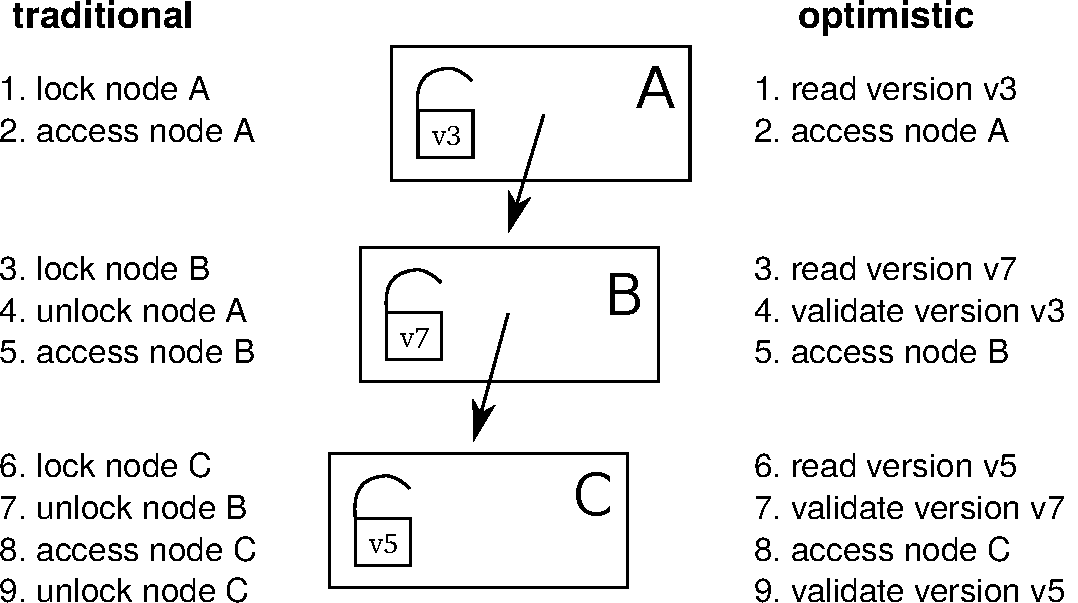
\includegraphics[width=0.65\linewidth]{olcall.pdf}
  \vspace{0.2cm}
  \caption{Comparison of a lookup operation in a 3-level tree using traditional lock coupling (left-hand side) vs.~optimistic lock coupling (right-hand side).}
  \label{fig:olc}
\end{figure}

The traditional and most common lock-based synchronization protocol for B-trees is lock coupling, which interleaves lock acquisitions while holding at most two locks at a time.
If, as we observed earlier, optimistic locks have similar semantics as traditional locks, it is natural to ask whether lock coupling can be combined with optimistic locks.
And indeed the answer is yes: One can almost mechanically translate traditional lock coupling code to optimistic lock coupling code.
This is illustrated in Figure~\ref{fig:olc}, which compares the traversal in a tree of height 3 using traditional and optimistic locks.
As the figure shows, the main difference is that locking is translated to reading the version and that unlocking becomes validation of the previously read version.
This simple change provides efficient lock-free tree traversal without the need to design a complex synchronization protocol.

It is important to emphasize the conceptual simplicity of OLC in comparison to data structures that use custom protocols like the Bw-tree~\cite{DBLP:conf/icde/LevandoskiLS13a}.
To implement lock-free access, the Bw-tree requires an indirection table, delta nodes, complex splitting and merging logic, retry logic, etc.
OLC, on the other hand, can directly be applied to B-trees mostly by adding the appropriate optimistic locking code and without modifying the node layout itself.
Therefore, OpenBw-Tree, an open source implementation of the Bw-tree, requires an order of magnitude more code than a B-tree based on OLC\footnote{Both implementations are available on GitHub: \url{https://github.com/wangziqi2016/index-microbench}}.
Given how difficult it is to develop, validate, and debug lock-free code, simplicity is obviously a major advantage.

\subsection{Correctness Aspects}

\begin{figure}
  % \centering
  %[basicstyle=\normalsize\ttfamily,showstringspaces=false,columns=fullflexible,breaklines=false,breakatwhitespace=true,numbers=none,numberstyle=\small,style=C,keepspaces=true]
\begin{lstlisting}[basicstyle=\ttfamily,language=C++,numbers=left,numberstyle=\small]
std::atomic<BTreeNode*> root;

// search for key in B+tree, returns payload in resultOut
bool lookup(Key key, Value& resultOut) {
   BTreeNode* node = root.load();
   uint64_t nodeVersion = node->readLockOrRestart();
   if (node != root.load()) // make sure the root is still the root
      restart();

   BTreeInner<Key>* parent = nullptr;
   uint64_t parentVersion = 0;

   while (node->isInner()) {
      auto inner = (BTreeInner*)node;

      // unlock parent and make current node the parent
      if (parent)
         parent->readUnlockOrRestart(parentVersion);
      parent = inner;
      parentVersion = nodeVersion;

      // search for next node
      node = inner->findChild(key);
      // validate 'inner' to ensure that 'node' pointer is valid
      inner->checkOrRestart(nodeVersion);
      // now it safe to dereference 'node' pointer (read its version)
      nodeVersion = node->readLockOrRestart();
   }

   // search in leaf and retrieve payload
   auto leaf = (BTreeLeaf*)node;
   bool success = leaf->findValue(key, resultOut);

   // unlock everything
   if (parent)
      parent->readUnlockOrRestart(parentVersion);
   node->readUnlockOrRestart(nodeVersion);

   return success;
}
\end{lstlisting}
  \vspace{0.2cm}
  \caption{B-tree lookup code using OLC. For simplicity, the restart logic is not shown.}
  \label{fig:lookup}
\end{figure}

So far, we have introduced the high-level ideas behind OLC and have stressed its similarity to traditional lock coupling.
Let us now discuss some cases where the close similarity between lock coupling and OLC breaks down.
To make this more concrete, we show the B-tree lookup code in Figure~\ref{fig:lookup}.
In the code, \texttt{readLockOrRestart} reads the lock version and \texttt{readUnlockOrRestart} validates that the read was correct.

One issue with OLC is that any pointer speculatively read from a node may point to invalid memory (if that node is modified concurrently).
Dereferencing such a pointer (e.g., to read its optimistic lock), may cause a segmentation fault or undefined behavior.
In the code shown in Figure~\ref{fig:lookup}, this problem is prevented by the extra check in line 25, which ensures that the read from the node containing the pointer was correct.
Without this additional validation, the code would in line 27 dereference the pointer speculatively read in line 23.
Note that the implementation of \texttt{checkOrRestart} is actually identical to \texttt{readUnlockOrRestart}.
We chose to give it a different name to highlight the fact that this extra check would not be necessary with read/write locks.

Another potential issue with optimistic locks is code that does not terminate.
Code that speculatively accesses a node, like an intra-node binary search, should be written in a way such that it always terminates---even in the presence of concurrent writes.
Otherwise, the validation code that detects the concurrent write will never run.
The binary search of a B-tree, for example, needs to be written in such a way that each comparison makes progress.
For some data structures that do not require loops in the traversal code (like ART) termination is trivially true.

\subsection{Implementation Details}

% implementation, efficiency
To implement an optimistic lock, one can combine the lock and the version counter into a single 64-bit\footnote{Even after subtracting one bit for the lock status, a back-of-the-envelope calculation can show that 63 bits are large enough to never overflow in practice.} word~\cite{artsync}.
A typical read operation will therefore merely consist of reading this version counter atomically.
In C++11 this can be implemented using the \texttt{std::atomic} type.

On x86, atomic reads are cheap because of x86's strong memory order guarantees.
No memory fences are required for sequentially-consistent loads, which are translated (by both GCC and clang) into standard \texttt{MOV} instructions.
Hence, the only effect of \texttt{std::atomic} for loads is preventing instruction re-ordering.
This makes version access and validation cheap.
Acquiring and releasing an optimistic lock in exclusive mode has comparable cost to a traditional lock:
A fairly expensive sequentially-consistent store is needed for acquiring a lock, while a standard \texttt{MOV} suffices for releasing it.
A simple sinlock-based implementation of optimistic locks can be found in the appendix of an earlier paper~\cite{artsync}.

OLC code must be able to handle restarts since validation or lock upgrade can fail due to concurrent writers.
Restarts can easily be implemented by wrapping the data structure operation in a loop (for simplicity not shown in Figure~\ref{fig:lookup}).
Such a loop also enables limiting the number of optimistic retry operations and falling back to pessimistic locking in cases of very heavy contention.
The ability to fall back to traditional locking is a major advantage of OLC in terms of robustness over lock-free approaches, which do not have this option.

In addition to the optimistic shared mode and the exclusive mode, optimistic locks also support a ``shared pessimistic'' mode, which physically acquires the lock in shared mode (allowing multiple concurrent readers but no writers).
This mode is useful for table (or range) scans that touch many tuples on a leaf page (which would otherwise easily abort).
Finally, let us mention that large range scans and table scans, should be broken up into several per-node traversals as is done in the LeanStore~\cite{leanstore} system.

Like all lock-free data structures, but unlike traditional locking and Hardware Transactional Memory~\cite{DBLP:conf/hpca/KarnagelDRLLSL14,DBLP:journals/pvldb/MakreshanskiLS15,htmtkde}, OLC requires care when deleting (and reusing) nodes.
The reason is that a deleting thread can never be sure that a node can be reclaimed because other threads might still be optimistically reading from that node.
Therefore, standard solutions like epoch-based reclamation~\cite{DBLP:conf/sosp/TuZKLM13}, hazard pointers~\cite{DBLP:journals/tpds/Michael04}, or optimized hazard pointers~\cite{DBLP:conf/spaa/BalmauGHZ16} need to be used.
These memory reclamation techniques are, however, largely orthogonal to the synchronization protocol itself.

%-lock-free is not a strong guarantee

\newpage
\section{Evaluation}\label{sec:evaluation}

Let us now experimentally evaluate the overhead and scalability of OLC.
For the experiments, we use an in-memory B+tree implemented in C++11 using templates, which is configured to use nodes of 4096 bytes, random 8 byte keys, and 8 byte payloads.
Based on this B-tree, we compare the following synchronization approaches:
\begin{itemize}
\item an OLC implementation\footnote{An almost identical OLC implementation is available on github: \url{https://github.com/wangziqi2016/index-microbench/tree/master/BTreeOLC}}
\item a variant based on traditional lock coupling and read/write locks
\item the unsynchronized B-tree, which obviously is only correct for read-only workloads but allows measuring the overhead of synchronization
\end{itemize}
Note that earlier work has compared the OLC implementation with a Bw-tree implementation~\cite{buzzword} and other state-of-the-art in-memory index structures.

We use a Haswell EP system with an Intel Xeon E5-2687W v3 CPU, which has 10 cores (20 ``Hyper-Threads'') and 25~MB of L3 cache.
The system is running Ubuntu 18.10 and we use GCC 8.2.0 to compile our code.
The CPU counters are obtained using the Linux perf API\footnote{We use the following convenience wrapper: \url{https://github.com/viktorleis/perfevent}}.

\begin{table}
  \caption{Performance and CPU counters for lookup and insert operations in a B-tree with 100M keys. We perform 100M operations and normalize the CPU counters by that number.}
  \label{tab:overhead}
  \centering
  \begin{tabular}{lrrrrrrr}\toprule
                    &         &        &        & instruc-  & L1     & L3     & branch \\
                    & threads & M op/s & cycles & tions & misses & misses & misses \\\midrule
lookup (no sync.)   & 1       & 1.72   & 2028   & 283     & 39.1   & 14.9   & 16.1   \\
lookup (OLC)        & 1       & 1.65   & 2107   & 370     & 43.9   & 15.1   & 16.7   \\
lookup (lock coup.) & 1       & 1.72   & 2078   & 365     & 42.3   & 16.9   & 15.7   \\\midrule
insert (no sync.)   & 1       & 1.51   & 2286   & 530     & 59.8   & 31.1   & 17.3   \\
insert (OLC)        & 1       & 1.50   & 2303   & 629     & 61.2   & 31.1   & 16.5   \\
insert (lock coup.) & 1       & 1.41   & 2473   & 644     & 61.0   & 31.0   & 17.2   \\\midrule
lookup (no sync.)   & 10      & 15.48  & 2058   & 283     & 38.6   & 15.5   & 16.0   \\
lookup (OLC)        & 10      & 14.60  & 2187   & 370     & 43.8   & 15.8   & 16.8   \\
lookup (lock coup.) & 10      & 5.71   & 5591   & 379     & 54.2   & 17.0   & 14.8   \\\midrule
insert (no sync.)   & 10      & -      & -      & -       & -      & -      & -      \\
insert (OLC)        & 10      & 10.46  & 2940   & 656     & 62.0   & 32.5   & 16.8   \\
insert (lock coup.) & 10      & 7.55   & 4161   & 667     & 75.0   & 28.6   & 16.2   \\
    \bottomrule
\end{tabular}
\end{table}

Table~\ref{tab:overhead} compares the performance and CPU counters for lookup and insert operations in a B-tree with 100M keys.
With {\em single-threaded} execution, we observe that all three approaches have very similar performance.
Adding traditional or optimistic locks to unsynchronized B-tree code results in up to 30\% of additional instructions without affecting single-threaded performance much.

\begin{figure}
  \centering
  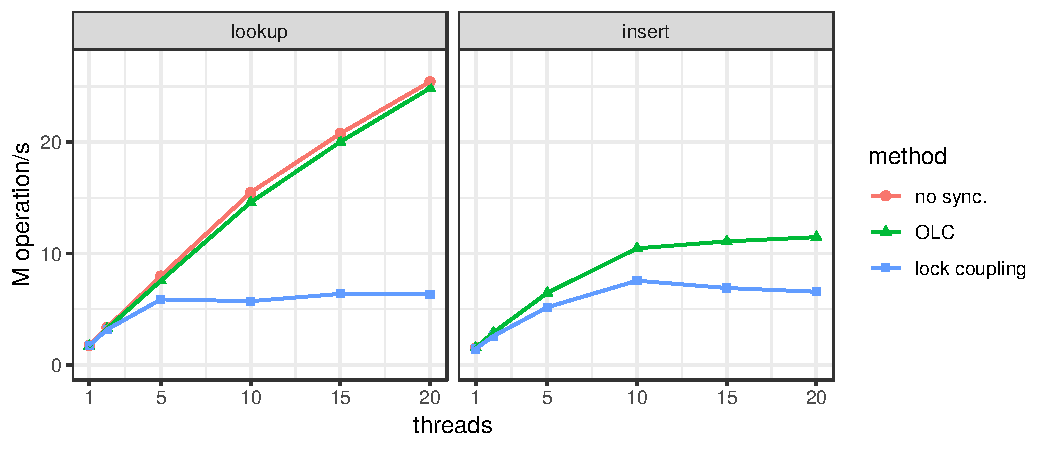
\includegraphics[width=\linewidth]{scale.pdf}
  \vspace{0.2cm}
  \caption{Scalability on 10-core system for B-tree operations (100M values).}
  \label{fig:scale}
\end{figure}

As Figure~\ref{fig:scale} shows, the results change dramatically once we use multiple threads.
For lookup, the scalability of OLC is near-linear up to 20 threads, even though the system has only 10 ``real cores''.
The OLC scalability for insert is also respectable (though not quite as linear because multi-threaded insertion approaches the memory bandwidth of our processor).
The figure also shows that the results of traditional lock coupling with read/write locks are significantly worse than OLC.
With 20 threads, lookup with OLC is 3.9$\times$ faster than traditional lock coupling.

\section{Summary}\label{sec:conc}

Optimistic Lock Coupling (OLC) is an effective synchronization method that combines the simplicity of traditional lock coupling with the superior scalability of lock-free approaches.
OLC is widely applicable and has already been successfully used to synchronize several data structures, including B-trees, binary search trees, and different trie variants.
These features make it highly attractive for modern database systems as well as performance-critical systems software in general.

\begin{thebibliography}{10}

\bibitem{DBLP:conf/spaa/BalmauGHZ16}
O.~Balmau, R.~Guerraoui, M.~Herlihy, and I.~Zablotchi.
\newblock Fast and robust memory reclamation for concurrent data structures.
\newblock In {\em SPAA}, 2016.

\bibitem{DBLP:journals/acta/BayerS77}
R.~Bayer and M.~Schkolnick.
\newblock Concurrency of operations on {B}-trees.
\newblock {\em Acta Informatica}, 9, 1977.

\bibitem{hot}
R.~Binna, E.~Zangerle, M.~Pichl, G.~Specht, and V.~Leis.
\newblock {HOT}: A height optimized trie index for main-memory database
  systems.
\newblock In {\em SIGMOD}, 2018.

\bibitem{DBLP:conf/ppopp/BronsonCCO10}
N.~G. Bronson, J.~Casper, H.~Chafi, and K.~Olukotun.
\newblock A practical concurrent binary search tree.
\newblock In {\em PPOPP}, 2010.

\bibitem{DBLP:conf/vldb/ChaHKK01}
S.~K. Cha, S.~Hwang, K.~Kim, and K.~Kwon.
\newblock Cache-conscious concurrency control of main-memory indexes on
  shared-memory multiprocessor systems.
\newblock In {\em VLDB}, 2001.

\bibitem{intel}
I.~Cutress.
\newblock {Intel} goes for 48-cores: {Cascade-AP} with multi-chip package
  coming soon.
\newblock
  \url{https://www.anandtech.com/show/13535/intel-goes-for-48cores-cascade-ap},
  2018 (accessed January, 2019).

\bibitem{DBLP:conf/cidr/FaleiroA17}
J.~M. Faleiro and D.~J. Abadi.
\newblock Latch-free synchronization in database systems: Silver bullet or
  fool's gold?
\newblock In {\em CIDR}, 2017.

\bibitem{DBLP:journals/ftdb/Graefe11}
G.~Graefe.
\newblock Modern {B}-tree techniques.
\newblock {\em Foundations and Trends in Databases}, 3(4), 2011.

\bibitem{DBLP:conf/hpca/KarnagelDRLLSL14}
T.~Karnagel, R.~Dementiev, R.~Rajwar, K.~Lai, T.~Legler, B.~Schlegel, and
  W.~Lehner.
\newblock Improving in-memory database index performance with
  {Intel}\({}^{\mbox{{\textregistered}}}\) transactional synchronization
  extensions.
\newblock In {\em HPCA}, 2014.

\bibitem{DBLP:journals/tods/LehmanY81}
P.~L. Lehman and S.~B. Yao.
\newblock Efficient locking for concurrent operations on {B}-trees.
\newblock {\em {ACM} Trans. Database Syst.}, 6(4), 1981.

\bibitem{leanstore}
V.~Leis, M.~Haubenschild, A.~Kemper, and T.~Neumann.
\newblock Leanstore: In-memory data management beyond main memory.
\newblock In {\em ICDE}, 2018.

\bibitem{art}
V.~Leis, A.~Kemper, and T.~Neumann.
\newblock The adaptive radix tree: {ARTful} indexing for main-memory databases.
\newblock In {\em ICDE}, 2013.

\bibitem{htmtkde}
V.~Leis, A.~Kemper, and T.~Neumann.
\newblock Scaling {HTM}-supported database transactions to many cores.
\newblock {\em {IEEE} Trans. Knowl. Data Eng.}, 28(2), 2016.

\bibitem{artsync}
V.~Leis, F.~Scheibner, A.~Kemper, and T.~Neumann.
\newblock The {ART} of practical synchronization.
\newblock In {\em DaMoN}, 2016.

\bibitem{DBLP:conf/icde/LevandoskiLS13a}
J.~J. Levandoski, D.~B. Lomet, and S.~Sengupta.
\newblock The {Bw}-tree: A {B}-tree for new hardware platforms.
\newblock In {\em ICDE}, 2013.

\bibitem{DBLP:journals/pvldb/MakreshanskiLS15}
D.~Makreshanski, J.~J. Levandoski, and R.~Stutsman.
\newblock To lock, swap, or elide: On the interplay of hardware transactional
  memory and lock-free indexing.
\newblock {\em {PVLDB}}, 8(11), 2015.

\bibitem{DBLP:dblp_conf/eurosys/MaoKM12}
Y.~Mao, E.~Kohler, and R.~T. Morris.
\newblock Cache craftiness for fast multicore key-value storage.
\newblock In {\em EuroSys}, 2012.

\bibitem{DBLP:journals/tpds/Michael04}
M.~M. Michael.
\newblock Hazard pointers: Safe memory reclamation for lock-free objects.
\newblock {\em {IEEE} Trans. Parallel Distrib. Syst.}, 15(6), 2004.

\bibitem{DBLP:journals/jacm/ShalevS06}
O.~Shalev and N.~Shavit.
\newblock Split-ordered lists: Lock-free extensible hash tables.
\newblock {\em J. {ACM}}, 53(3), 2006.

\bibitem{amd}
A.~Shilov.
\newblock {AMD} previews {EPYC} ‘{Rome}’ processor: Up to 64 {Zen} 2 cores.
\newblock
  \url{https://www.anandtech.com/show/13561/amd-previews-epyc-rome-processor-up-to-64-zen-2-cores},
  2018 (accessed January, 2019).

\bibitem{DBLP:conf/sosp/TuZKLM13}
S.~Tu, W.~Zheng, E.~Kohler, B.~Liskov, and S.~Madden.
\newblock Speedy transactions in multicore in-memory databases.
\newblock In {\em SOSP}, 2013.

\bibitem{buzzword}
Z.~Wang, A.~Pavlo, H.~Lim, V.~Leis, H.~Zhang, M.~Kaminsky, and D.~Andersen.
\newblock Building a {Bw}-tree takes more than just buzz words.
\newblock In {\em SIGMOD}, 2018.

\end{thebibliography}


%\bibliographystyle{abbrv}
%\bibliography{main}

\end{document}

\end{article}

\begin{article}
{Enhance Mono-modal Sentiment Classification with Federated Cross-modal Transfer}
{Xueyang Wu, Di Jiang, Yuanfeng Song, Qian Xu, and Qiang Yang}
\pdfminorversion=5
\documentclass[11pt]{article}
\usepackage{deauthor,times,graphicx,caption,microtype}
\usepackage{hyperref}
\usepackage{listings}
\usepackage{booktabs}

\begin{document}

\title{Optimistic Lock Coupling: A Scalable and Efficient General-Purpose Synchronization Method}

\author{Viktor Leis, Michael Haubenschild\raisebox{0.9ex}{$\ast$}, Thomas Neumann\\ Technische Universit{\"a}t M{\"u}nchen \hspace{0.7cm} Tableau Software\raisebox{0.9ex}{$\ast$} \\ {\{leis,neumann\}{@}in.tum.de} \hspace{0.7cm} {mhaubenschild{@}tableau.com\raisebox{0.9ex}{$\ast$}}}

\maketitle

\begin{abstract}
As the number of cores on commodity processors continues to increase, scalability becomes more and more crucial for overall performance.
Scalable and efficient concurrent data structures are particularly important, as these are often the building blocks of parallel algorithms.
Unfortunately, traditional synchronization techniques based on fine-grained locking have been shown to be unscalable on modern multi-core CPUs.
Lock-free data structures, on the other hand, are extremely difficult to design and often incur significant overhead.

In this work, we make the case for Optimistic Lock Coupling as a practical alternative to both traditional locking and the lock-free approach.
We show that Optimistic Lock Coupling is highly scalable and almost as simple to implement as traditional lock coupling.
Another important advantage is that it is easily applicable to most tree-like data structures.
We therefore argue that Optimistic Lock Coupling, rather than a complex and error-prone custom synchronization protocol, should be the default choice for performance-critical data structures.
\end{abstract}

\section{Introduction}

% more and more cores
Today, Intel's commodity server processors have up to 28 cores and its upcoming microarchitecture will have up to 48 cores per socket~\cite{intel}.
Similarly, AMD currently stands at 32 cores and this number is expected to double in the next generation~\cite{amd}.
Since both platforms support simultaneous multithreading (also known as hyperthreading), affordable commodity servers (with up to two sockets) will soon routinely have between 100 and 200 hardware threads.

% data structure scalability is important
With such a high degree of hardware parallelism, efficient data processing crucially depends on how well concurrent data structures scale.
Internally, database systems use a plethora of data structures like table heaps, internal work queues, and, most importantly, index structures.
Any of these can easily become a scalability (and therefore overall performance) bottleneck on many-core CPUs.

% traditional synchronization: fine-grained locks, slow, cache invalidation
Traditionally, database systems synchronize internal data structures using fine-grained reader/writer locks\footnote{In this work, we focus on data structure synchronization rather than high-level transaction semantics and therefore use the term {\em lock} for what would typically be called {\em latch} in the database literature. We thus follow common computer science (rather than database) terminology.}.
Unfortunately, while fine-grained locking makes lock contention unlikely, it still results in bad scalability because lock acquisition and release require writing to shared memory.
Due to the way cache coherency is implemented on modern multi-core CPUs, these writes cause additional cache misses\footnote{The cache coherency protocol ensures that all copies of a cache line on other cores are invalidated before the write can proceed.} and the cache line containing the lock's internal data becomes a point of physical contention.
As a result, any frequently-accessed lock (e.g., the lock of the root node of a B-tree) severely limits scalability.

% lock-free bw-tree: no more latches, but indirections, extremely complex
Lock-free data structures like the Bw-tree~\cite{DBLP:conf/icde/LevandoskiLS13a} (a lock-free B-tree variant) or the Split-Ordered List~\cite{DBLP:journals/jacm/ShalevS06} (a lock-free hash table) do not acquire any locks and therefore generally scale much better than locking-based approaches (in particular for read-mostly workloads).
However, lock-free synchronization has other downsides:
First, it is very difficult and results in extremely complex and error-prone code (when compared to locking).
Second, because the functionality of atomic primitives provided by the hardware (e.g., atomically compare-and-swap 8 bytes) is limited, complex operations require additional indirections within the data structure.
For example, the Bw-tree requires an indirection table and the Split-Ordered List requires ``dummy nodes'', resulting in overhead due to additional cache misses.

% OLC for the win
In this paper we make the case for {\em Optimistic Lock Coupling (OLC)}, a synchronization method that combines some of the best properties of lock-based and lock-free synchronization.
OLC utilizes a special lock type that can be used in two modes:
The first mode is similar to a traditional mutex and excludes other threads by physically acquiring the underlying lock.
In the second mode, reads can proceed optimistically by validating a version counter that is embedded in the lock (similar to optimistic concurrency control).
The first mode is typically used by writers and the second mode by readers.
Besides this special lock type, OLC is based on the observation that optimistic lock validations can be interleaved/coupled---similar to the pair-wise interleaved lock acquisition of traditional lock coupling.
Hence, the name Optimistic Lock Coupling.

OLC has a number of desirable features:
\begin{itemize}
\item By reducing the number of writes to shared memory locations and thereby avoiding cache invalidations, it {\bf scales well} for most workloads.
\item In comparison to unsynchronized code, it requires few additional CPU instructions making it {\bf efficient}.
\item OLC is {\bf widely applicable} to different data structures. It has already been successfully used for synchronizing binary search trees~\cite{DBLP:conf/ppopp/BronsonCCO10}, tries~\cite{artsync}, trie/B-tree hybrids~\cite{DBLP:dblp_conf/eurosys/MaoKM12}, and B-trees~\cite{buzzword}.
\item In comparison to the lock-free paradigm, it is also {\bf easy to use} and requires few modifications to existing, single-threaded data structures.
\end{itemize}
Despite these positive features and its simplicity, OLC is not yet widely known.
The goal of this paper is therefore to popularize this simple idea and to make a case for it.
We argue that OLC deserves to be widely known.
It is a good default synchronization paradigm---more complex, data structure-specific protocols are seldom beneficial.

The rest of the paper is organized as follows.
Section~\ref{sec:related} discusses related work, tracing the history of OLC and its underlying ideas in the literature.
The core of the paper is Section~\ref{sec:olc}, which describes the ideas behind OLC and how it can be used to synchronize complex data structures.
In Section~\ref{sec:evaluation} we experimentally show that OLC has low overhead and scales well when used to synchronize an in-memory B-tree.
We summarize the paper in Section~\ref{sec:conc}.

\newpage
\section{Related Work}\label{sec:related}

Lock coupling has been proposed as a method for allowing concurrent operations on B-trees in 1977~\cite{DBLP:journals/acta/BayerS77}.
This traditional and still widely-used method, described in detail in Graefe's B-tree survey~\cite{DBLP:journals/ftdb/Graefe11}, is also called ``latch coupling'', ``hand-over-hand locking'', and ``crabbing''.
Because at most two locks are held at-a-time during tree traversal, this technique seemingly allows for a high degree of parallelism---in particular if read/write locks are used to enable inner nodes to be locked in shared mode.
However, as we show in Section~\ref{sec:evaluation}, on modern hardware lock acquisition (even in shared mode) results in suboptimal scalability.

An early alternative from 1981 is a B-tree variant called B-link tree~\cite{DBLP:journals/tods/LehmanY81}, which only holds a single lock at a time.
It is based on the observation that between the release of the parent lock and the acquisition of the child lock, the only ``dangerous'' thing that could have happened is the split of a child node (assuming one does not implement merge operations).
Thus, when a split happens, the key being searched might end up on a neighboring node to the right of the current child node.
A B-link tree traversal therefore detects this condition and, if needed, transparently proceeds to the neighboring node.
Releasing the parent lock early is highly beneficial when the child node needs to be fetched from disk.
For in-memory workloads, however, the B-link tree has the same scalability issues as lock coupling (it acquires just as many locks).

The next major advance, Optimistic Latch-Free Index Traversal (OLFIT)~\cite{DBLP:conf/vldb/ChaHKK01}, was proposed in 2001.
OLFIT introduced the idea of a combined lock/update counter, which we call {\em optimistic lock}. % , for lack of a better name,
Based on these per-node optimistic locks and the synchronization protocol of the B-link tree, OLFIT finally achieves good scalability on parallel processors.
The OLFIT protocol is fairly complex, as it requires both the non-trivial B-link protocol and optimistic locks.
Furthermore, like the B-link tree protocol, it does not support merging nodes, and is specific to B-trees (cannot easily be applied to other data structures).

In the following two decades, the growth of main-memory capacity led to much research into other data structures besides the venerable B-tree.
Particularly relevant for our discussion is Bronson et al.'s~\cite{DBLP:conf/ppopp/BronsonCCO10} concurrent binary search tree, which is based on optimistic version validation and has a sophisticated, data structure-specific synchronization protocol.
To the best of our knowledge, this 2010 paper is the first that, as part of its protocol, interleaves version validation across nodes---rather than validating each node separately like OLFIT.
In that paper, this idea is called ``hand-over-hand, optimistic validation'', while we prefer the term Optimistic Lock Coupling to highlight the close resemblance to traditional lock coupling.
Similarly, Mao et al.'s~\cite{DBLP:dblp_conf/eurosys/MaoKM12} Masstree (a concurrent hybrid trie/B-tree) is also based on the same ideas, but again uses them as part of a more complex protocol.

The Adaptive Radix Tree (ART)~\cite{art} is another recent in-memory data structure, which we proposed in 2013.
In contrast to the two data structures just mentioned, it was originally designed with single-threaded performance in mind without supporting concurrency.
To add support for concurrency, we initially started designing a custom protocol called Read-Optimized Write Exclusion (ROWEX)~\cite{artsync}, which turned out to be non-trivial and requires modifications of the underlying data structure\footnote{Note that ROWEX is already easier to apply to existing data structures than the lock-free approach. The difficulty depends on the data structure. Applying ROWEX is hard for B-trees with sorted keys and fairly easy for copy-on-write data structures like the Height Optimized Trie~\cite{hot}---with ART being somewhere in the middle.}.
However, fairly late in the project, we also realized, that OLC {\em alone} (rather than as part of a more complex protocol) is sufficient to synchronize ART.
No other changes to the data structure were necessary.
Both approaches were published and experimentally evaluated in a followup paper~\cite{artsync}, which shows that, despite its simplicity, OLC is efficient, scalable, and generally outperforms ROWEX.

Similar results were recently published regarding B-trees~\cite{buzzword}.
In this experimental study a simple OLC-based synchronization outperformed the Bw-tree~\cite{DBLP:conf/icde/LevandoskiLS13a}, a complex lock-free synchronization approach.
Another recent paper shows that for write-intensive workloads, locking often performs better than lock-free synchronization~\cite{DBLP:conf/cidr/FaleiroA17}.
These experiences indicate that OLC is a general-purpose synchronization paradigm and motivate the current paper.

%foster b-tree\cite{DBLP:journals/tods/GraefeKK12}
%Shasha theory~\cite{DBLP:journals/tods/ShashaG88}

\section{Optimistic Lock Coupling}\label{sec:olc}

% locks suck
The standard technique for inter-thread synchronization is mutual exclusion using fine-grained locks.
In a B-tree, for example, every node usually has its own associated lock, which is acquired before accessing that node.
The problem of locking on modern multi- and many-core processors is that lock acquisition and release require writing to the shared memory location that implements the lock.
This write causes exclusive ownership of the underlying cache line and invalidates copies of it on all other processor cores.
For hierarchical, tree-like data structures, the lock of the root node becomes a point of physical contention---even in read-only workloads and even when read/write locks are used.
Depending on the specific data structure, number of cores, cache coherency protocol implementation, cache topology, whether Non-Uniform Memory Access (NUMA) is used, locking can even result in multi-threaded performance that is worse than single-threaded execution.

% in b-trees this happens very much
The inherent pessimism of locking is particularly unfortunate for B-trees:
Despite the fact that logical modifications of the root node are very infrequent, every B-tree operation must lock the root node during tree traversal\footnote{To a lesser extent this obviously applies to all inner nodes, not just the root.}.
Even the vast majority of update operations (with the exception of splits and merges), only modify a single leaf node.
These observations indicate that a more optimistic approach, which does not require locking inner nodes, would be very beneficial for B-trees.

\subsection{Optimistic Locks}

% optimism to the rescue
As the name indicates, optimistic locks try to solve the scalability issues of traditional locks using an optimistic approach.
Instead of always physically acquiring locks, even for nodes that are unlikely to be modified simultaneously, after-the-fact validation is used to detect conflicts.
This is done by augmenting each lock with a version/update counter that is incremented on every modification.
Using this version counter, readers can optimistically proceed before validating that the version did not change to ensure that the read was safe.
If validation fails, the operation is restarted.

% details on opt locks
Using optimistic locks, a read-only node access (i.e., the majority of all operations in a B-tree) does not acquire the lock and does not increment the version counter.
Instead, it performs the following steps:
\begin{enumerate}
\item read lock version (restart if lock is not free)
\item access node
\item read the version again and validate that it has not changed in the meantime
\end{enumerate}
If the last step (the validation) fails, the operation has to be restarted.
Write operations, on the other hand, are more similar to traditional locking:
\begin{enumerate}
\item acquire lock (wait if necessary)
\item access/write to node
\item increment version and unlock node
\end{enumerate}
Writes can therefore protect a node from other writes.

% similar to locks
As we observed in an earlier paper~\cite{artsync}, because of similar semantics, optimistic locks can be hidden behind an API very similar to traditional read/write locks.
Both approaches have an exclusive lock mode, and acquiring a traditional lock in shared mode is analogous to optimistic version validation.
Furthermore, like with some implementations of traditional read/write locks, optimistic locks allow upgrading a shared lock to an exclusive lock.
Lock upgrades are, for example, used to avoid most B-tree update operations from having to lock inner nodes.
In our experience, the close resemblance of optimistic and traditional locks simplifies the reasoning about optimistic locks;
one can apply similar thinking as in traditional lock-based protocols.

\subsection{Lock Coupling with Optimistic Locks}

\begin{figure}
  \centering
  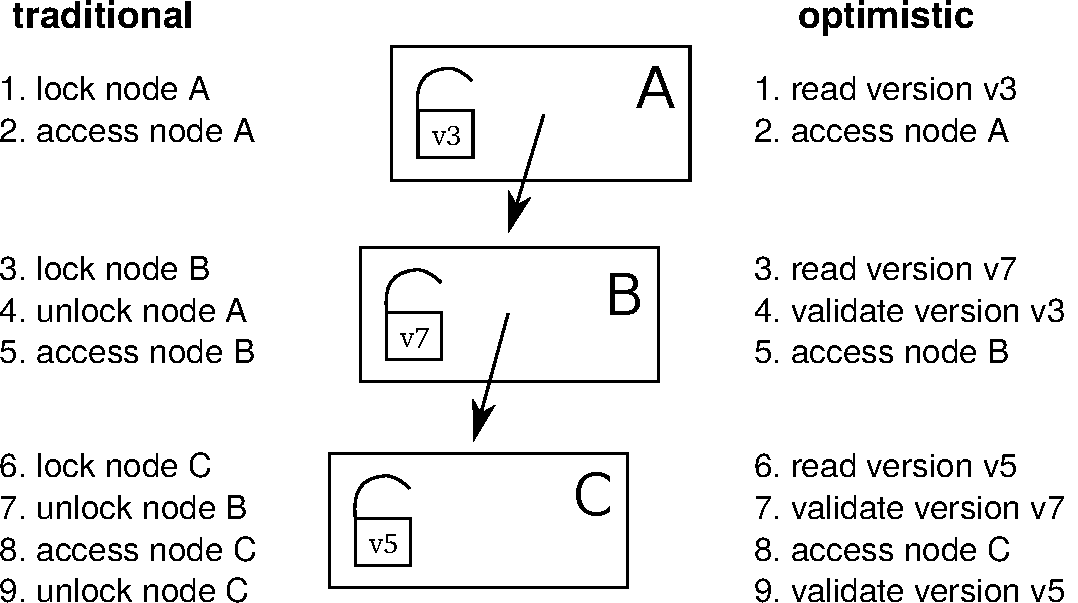
\includegraphics[width=0.65\linewidth]{olcall.pdf}
  \vspace{0.2cm}
  \caption{Comparison of a lookup operation in a 3-level tree using traditional lock coupling (left-hand side) vs.~optimistic lock coupling (right-hand side).}
  \label{fig:olc}
\end{figure}

The traditional and most common lock-based synchronization protocol for B-trees is lock coupling, which interleaves lock acquisitions while holding at most two locks at a time.
If, as we observed earlier, optimistic locks have similar semantics as traditional locks, it is natural to ask whether lock coupling can be combined with optimistic locks.
And indeed the answer is yes: One can almost mechanically translate traditional lock coupling code to optimistic lock coupling code.
This is illustrated in Figure~\ref{fig:olc}, which compares the traversal in a tree of height 3 using traditional and optimistic locks.
As the figure shows, the main difference is that locking is translated to reading the version and that unlocking becomes validation of the previously read version.
This simple change provides efficient lock-free tree traversal without the need to design a complex synchronization protocol.

It is important to emphasize the conceptual simplicity of OLC in comparison to data structures that use custom protocols like the Bw-tree~\cite{DBLP:conf/icde/LevandoskiLS13a}.
To implement lock-free access, the Bw-tree requires an indirection table, delta nodes, complex splitting and merging logic, retry logic, etc.
OLC, on the other hand, can directly be applied to B-trees mostly by adding the appropriate optimistic locking code and without modifying the node layout itself.
Therefore, OpenBw-Tree, an open source implementation of the Bw-tree, requires an order of magnitude more code than a B-tree based on OLC\footnote{Both implementations are available on GitHub: \url{https://github.com/wangziqi2016/index-microbench}}.
Given how difficult it is to develop, validate, and debug lock-free code, simplicity is obviously a major advantage.

\subsection{Correctness Aspects}

\begin{figure}
  % \centering
  %[basicstyle=\normalsize\ttfamily,showstringspaces=false,columns=fullflexible,breaklines=false,breakatwhitespace=true,numbers=none,numberstyle=\small,style=C,keepspaces=true]
\begin{lstlisting}[basicstyle=\ttfamily,language=C++,numbers=left,numberstyle=\small]
std::atomic<BTreeNode*> root;

// search for key in B+tree, returns payload in resultOut
bool lookup(Key key, Value& resultOut) {
   BTreeNode* node = root.load();
   uint64_t nodeVersion = node->readLockOrRestart();
   if (node != root.load()) // make sure the root is still the root
      restart();

   BTreeInner<Key>* parent = nullptr;
   uint64_t parentVersion = 0;

   while (node->isInner()) {
      auto inner = (BTreeInner*)node;

      // unlock parent and make current node the parent
      if (parent)
         parent->readUnlockOrRestart(parentVersion);
      parent = inner;
      parentVersion = nodeVersion;

      // search for next node
      node = inner->findChild(key);
      // validate 'inner' to ensure that 'node' pointer is valid
      inner->checkOrRestart(nodeVersion);
      // now it safe to dereference 'node' pointer (read its version)
      nodeVersion = node->readLockOrRestart();
   }

   // search in leaf and retrieve payload
   auto leaf = (BTreeLeaf*)node;
   bool success = leaf->findValue(key, resultOut);

   // unlock everything
   if (parent)
      parent->readUnlockOrRestart(parentVersion);
   node->readUnlockOrRestart(nodeVersion);

   return success;
}
\end{lstlisting}
  \vspace{0.2cm}
  \caption{B-tree lookup code using OLC. For simplicity, the restart logic is not shown.}
  \label{fig:lookup}
\end{figure}

So far, we have introduced the high-level ideas behind OLC and have stressed its similarity to traditional lock coupling.
Let us now discuss some cases where the close similarity between lock coupling and OLC breaks down.
To make this more concrete, we show the B-tree lookup code in Figure~\ref{fig:lookup}.
In the code, \texttt{readLockOrRestart} reads the lock version and \texttt{readUnlockOrRestart} validates that the read was correct.

One issue with OLC is that any pointer speculatively read from a node may point to invalid memory (if that node is modified concurrently).
Dereferencing such a pointer (e.g., to read its optimistic lock), may cause a segmentation fault or undefined behavior.
In the code shown in Figure~\ref{fig:lookup}, this problem is prevented by the extra check in line 25, which ensures that the read from the node containing the pointer was correct.
Without this additional validation, the code would in line 27 dereference the pointer speculatively read in line 23.
Note that the implementation of \texttt{checkOrRestart} is actually identical to \texttt{readUnlockOrRestart}.
We chose to give it a different name to highlight the fact that this extra check would not be necessary with read/write locks.

Another potential issue with optimistic locks is code that does not terminate.
Code that speculatively accesses a node, like an intra-node binary search, should be written in a way such that it always terminates---even in the presence of concurrent writes.
Otherwise, the validation code that detects the concurrent write will never run.
The binary search of a B-tree, for example, needs to be written in such a way that each comparison makes progress.
For some data structures that do not require loops in the traversal code (like ART) termination is trivially true.

\subsection{Implementation Details}

% implementation, efficiency
To implement an optimistic lock, one can combine the lock and the version counter into a single 64-bit\footnote{Even after subtracting one bit for the lock status, a back-of-the-envelope calculation can show that 63 bits are large enough to never overflow in practice.} word~\cite{artsync}.
A typical read operation will therefore merely consist of reading this version counter atomically.
In C++11 this can be implemented using the \texttt{std::atomic} type.

On x86, atomic reads are cheap because of x86's strong memory order guarantees.
No memory fences are required for sequentially-consistent loads, which are translated (by both GCC and clang) into standard \texttt{MOV} instructions.
Hence, the only effect of \texttt{std::atomic} for loads is preventing instruction re-ordering.
This makes version access and validation cheap.
Acquiring and releasing an optimistic lock in exclusive mode has comparable cost to a traditional lock:
A fairly expensive sequentially-consistent store is needed for acquiring a lock, while a standard \texttt{MOV} suffices for releasing it.
A simple sinlock-based implementation of optimistic locks can be found in the appendix of an earlier paper~\cite{artsync}.

OLC code must be able to handle restarts since validation or lock upgrade can fail due to concurrent writers.
Restarts can easily be implemented by wrapping the data structure operation in a loop (for simplicity not shown in Figure~\ref{fig:lookup}).
Such a loop also enables limiting the number of optimistic retry operations and falling back to pessimistic locking in cases of very heavy contention.
The ability to fall back to traditional locking is a major advantage of OLC in terms of robustness over lock-free approaches, which do not have this option.

In addition to the optimistic shared mode and the exclusive mode, optimistic locks also support a ``shared pessimistic'' mode, which physically acquires the lock in shared mode (allowing multiple concurrent readers but no writers).
This mode is useful for table (or range) scans that touch many tuples on a leaf page (which would otherwise easily abort).
Finally, let us mention that large range scans and table scans, should be broken up into several per-node traversals as is done in the LeanStore~\cite{leanstore} system.

Like all lock-free data structures, but unlike traditional locking and Hardware Transactional Memory~\cite{DBLP:conf/hpca/KarnagelDRLLSL14,DBLP:journals/pvldb/MakreshanskiLS15,htmtkde}, OLC requires care when deleting (and reusing) nodes.
The reason is that a deleting thread can never be sure that a node can be reclaimed because other threads might still be optimistically reading from that node.
Therefore, standard solutions like epoch-based reclamation~\cite{DBLP:conf/sosp/TuZKLM13}, hazard pointers~\cite{DBLP:journals/tpds/Michael04}, or optimized hazard pointers~\cite{DBLP:conf/spaa/BalmauGHZ16} need to be used.
These memory reclamation techniques are, however, largely orthogonal to the synchronization protocol itself.

%-lock-free is not a strong guarantee

\newpage
\section{Evaluation}\label{sec:evaluation}

Let us now experimentally evaluate the overhead and scalability of OLC.
For the experiments, we use an in-memory B+tree implemented in C++11 using templates, which is configured to use nodes of 4096 bytes, random 8 byte keys, and 8 byte payloads.
Based on this B-tree, we compare the following synchronization approaches:
\begin{itemize}
\item an OLC implementation\footnote{An almost identical OLC implementation is available on github: \url{https://github.com/wangziqi2016/index-microbench/tree/master/BTreeOLC}}
\item a variant based on traditional lock coupling and read/write locks
\item the unsynchronized B-tree, which obviously is only correct for read-only workloads but allows measuring the overhead of synchronization
\end{itemize}
Note that earlier work has compared the OLC implementation with a Bw-tree implementation~\cite{buzzword} and other state-of-the-art in-memory index structures.

We use a Haswell EP system with an Intel Xeon E5-2687W v3 CPU, which has 10 cores (20 ``Hyper-Threads'') and 25~MB of L3 cache.
The system is running Ubuntu 18.10 and we use GCC 8.2.0 to compile our code.
The CPU counters are obtained using the Linux perf API\footnote{We use the following convenience wrapper: \url{https://github.com/viktorleis/perfevent}}.

\begin{table}
  \caption{Performance and CPU counters for lookup and insert operations in a B-tree with 100M keys. We perform 100M operations and normalize the CPU counters by that number.}
  \label{tab:overhead}
  \centering
  \begin{tabular}{lrrrrrrr}\toprule
                    &         &        &        & instruc-  & L1     & L3     & branch \\
                    & threads & M op/s & cycles & tions & misses & misses & misses \\\midrule
lookup (no sync.)   & 1       & 1.72   & 2028   & 283     & 39.1   & 14.9   & 16.1   \\
lookup (OLC)        & 1       & 1.65   & 2107   & 370     & 43.9   & 15.1   & 16.7   \\
lookup (lock coup.) & 1       & 1.72   & 2078   & 365     & 42.3   & 16.9   & 15.7   \\\midrule
insert (no sync.)   & 1       & 1.51   & 2286   & 530     & 59.8   & 31.1   & 17.3   \\
insert (OLC)        & 1       & 1.50   & 2303   & 629     & 61.2   & 31.1   & 16.5   \\
insert (lock coup.) & 1       & 1.41   & 2473   & 644     & 61.0   & 31.0   & 17.2   \\\midrule
lookup (no sync.)   & 10      & 15.48  & 2058   & 283     & 38.6   & 15.5   & 16.0   \\
lookup (OLC)        & 10      & 14.60  & 2187   & 370     & 43.8   & 15.8   & 16.8   \\
lookup (lock coup.) & 10      & 5.71   & 5591   & 379     & 54.2   & 17.0   & 14.8   \\\midrule
insert (no sync.)   & 10      & -      & -      & -       & -      & -      & -      \\
insert (OLC)        & 10      & 10.46  & 2940   & 656     & 62.0   & 32.5   & 16.8   \\
insert (lock coup.) & 10      & 7.55   & 4161   & 667     & 75.0   & 28.6   & 16.2   \\
    \bottomrule
\end{tabular}
\end{table}

Table~\ref{tab:overhead} compares the performance and CPU counters for lookup and insert operations in a B-tree with 100M keys.
With {\em single-threaded} execution, we observe that all three approaches have very similar performance.
Adding traditional or optimistic locks to unsynchronized B-tree code results in up to 30\% of additional instructions without affecting single-threaded performance much.

\begin{figure}
  \centering
  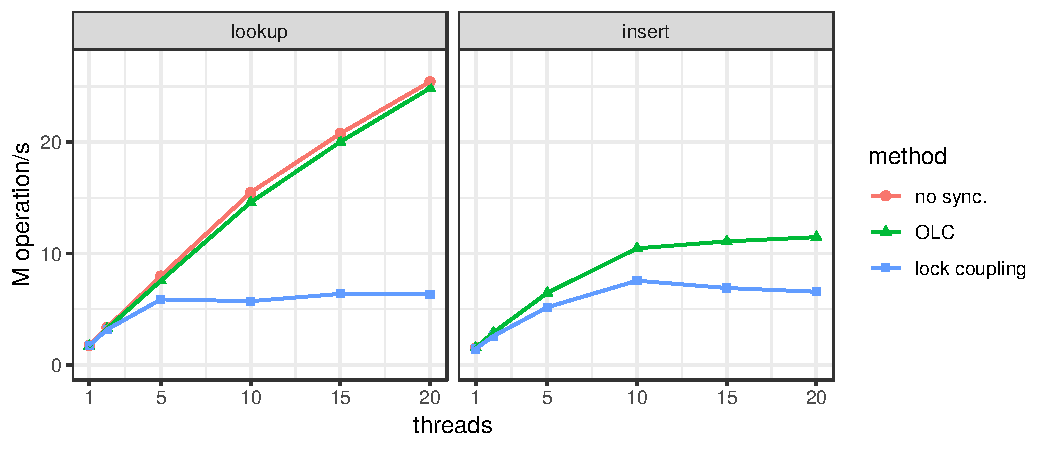
\includegraphics[width=\linewidth]{scale.pdf}
  \vspace{0.2cm}
  \caption{Scalability on 10-core system for B-tree operations (100M values).}
  \label{fig:scale}
\end{figure}

As Figure~\ref{fig:scale} shows, the results change dramatically once we use multiple threads.
For lookup, the scalability of OLC is near-linear up to 20 threads, even though the system has only 10 ``real cores''.
The OLC scalability for insert is also respectable (though not quite as linear because multi-threaded insertion approaches the memory bandwidth of our processor).
The figure also shows that the results of traditional lock coupling with read/write locks are significantly worse than OLC.
With 20 threads, lookup with OLC is 3.9$\times$ faster than traditional lock coupling.

\section{Summary}\label{sec:conc}

Optimistic Lock Coupling (OLC) is an effective synchronization method that combines the simplicity of traditional lock coupling with the superior scalability of lock-free approaches.
OLC is widely applicable and has already been successfully used to synchronize several data structures, including B-trees, binary search trees, and different trie variants.
These features make it highly attractive for modern database systems as well as performance-critical systems software in general.

\begin{thebibliography}{10}

\bibitem{DBLP:conf/spaa/BalmauGHZ16}
O.~Balmau, R.~Guerraoui, M.~Herlihy, and I.~Zablotchi.
\newblock Fast and robust memory reclamation for concurrent data structures.
\newblock In {\em SPAA}, 2016.

\bibitem{DBLP:journals/acta/BayerS77}
R.~Bayer and M.~Schkolnick.
\newblock Concurrency of operations on {B}-trees.
\newblock {\em Acta Informatica}, 9, 1977.

\bibitem{hot}
R.~Binna, E.~Zangerle, M.~Pichl, G.~Specht, and V.~Leis.
\newblock {HOT}: A height optimized trie index for main-memory database
  systems.
\newblock In {\em SIGMOD}, 2018.

\bibitem{DBLP:conf/ppopp/BronsonCCO10}
N.~G. Bronson, J.~Casper, H.~Chafi, and K.~Olukotun.
\newblock A practical concurrent binary search tree.
\newblock In {\em PPOPP}, 2010.

\bibitem{DBLP:conf/vldb/ChaHKK01}
S.~K. Cha, S.~Hwang, K.~Kim, and K.~Kwon.
\newblock Cache-conscious concurrency control of main-memory indexes on
  shared-memory multiprocessor systems.
\newblock In {\em VLDB}, 2001.

\bibitem{intel}
I.~Cutress.
\newblock {Intel} goes for 48-cores: {Cascade-AP} with multi-chip package
  coming soon.
\newblock
  \url{https://www.anandtech.com/show/13535/intel-goes-for-48cores-cascade-ap},
  2018 (accessed January, 2019).

\bibitem{DBLP:conf/cidr/FaleiroA17}
J.~M. Faleiro and D.~J. Abadi.
\newblock Latch-free synchronization in database systems: Silver bullet or
  fool's gold?
\newblock In {\em CIDR}, 2017.

\bibitem{DBLP:journals/ftdb/Graefe11}
G.~Graefe.
\newblock Modern {B}-tree techniques.
\newblock {\em Foundations and Trends in Databases}, 3(4), 2011.

\bibitem{DBLP:conf/hpca/KarnagelDRLLSL14}
T.~Karnagel, R.~Dementiev, R.~Rajwar, K.~Lai, T.~Legler, B.~Schlegel, and
  W.~Lehner.
\newblock Improving in-memory database index performance with
  {Intel}\({}^{\mbox{{\textregistered}}}\) transactional synchronization
  extensions.
\newblock In {\em HPCA}, 2014.

\bibitem{DBLP:journals/tods/LehmanY81}
P.~L. Lehman and S.~B. Yao.
\newblock Efficient locking for concurrent operations on {B}-trees.
\newblock {\em {ACM} Trans. Database Syst.}, 6(4), 1981.

\bibitem{leanstore}
V.~Leis, M.~Haubenschild, A.~Kemper, and T.~Neumann.
\newblock Leanstore: In-memory data management beyond main memory.
\newblock In {\em ICDE}, 2018.

\bibitem{art}
V.~Leis, A.~Kemper, and T.~Neumann.
\newblock The adaptive radix tree: {ARTful} indexing for main-memory databases.
\newblock In {\em ICDE}, 2013.

\bibitem{htmtkde}
V.~Leis, A.~Kemper, and T.~Neumann.
\newblock Scaling {HTM}-supported database transactions to many cores.
\newblock {\em {IEEE} Trans. Knowl. Data Eng.}, 28(2), 2016.

\bibitem{artsync}
V.~Leis, F.~Scheibner, A.~Kemper, and T.~Neumann.
\newblock The {ART} of practical synchronization.
\newblock In {\em DaMoN}, 2016.

\bibitem{DBLP:conf/icde/LevandoskiLS13a}
J.~J. Levandoski, D.~B. Lomet, and S.~Sengupta.
\newblock The {Bw}-tree: A {B}-tree for new hardware platforms.
\newblock In {\em ICDE}, 2013.

\bibitem{DBLP:journals/pvldb/MakreshanskiLS15}
D.~Makreshanski, J.~J. Levandoski, and R.~Stutsman.
\newblock To lock, swap, or elide: On the interplay of hardware transactional
  memory and lock-free indexing.
\newblock {\em {PVLDB}}, 8(11), 2015.

\bibitem{DBLP:dblp_conf/eurosys/MaoKM12}
Y.~Mao, E.~Kohler, and R.~T. Morris.
\newblock Cache craftiness for fast multicore key-value storage.
\newblock In {\em EuroSys}, 2012.

\bibitem{DBLP:journals/tpds/Michael04}
M.~M. Michael.
\newblock Hazard pointers: Safe memory reclamation for lock-free objects.
\newblock {\em {IEEE} Trans. Parallel Distrib. Syst.}, 15(6), 2004.

\bibitem{DBLP:journals/jacm/ShalevS06}
O.~Shalev and N.~Shavit.
\newblock Split-ordered lists: Lock-free extensible hash tables.
\newblock {\em J. {ACM}}, 53(3), 2006.

\bibitem{amd}
A.~Shilov.
\newblock {AMD} previews {EPYC} ‘{Rome}’ processor: Up to 64 {Zen} 2 cores.
\newblock
  \url{https://www.anandtech.com/show/13561/amd-previews-epyc-rome-processor-up-to-64-zen-2-cores},
  2018 (accessed January, 2019).

\bibitem{DBLP:conf/sosp/TuZKLM13}
S.~Tu, W.~Zheng, E.~Kohler, B.~Liskov, and S.~Madden.
\newblock Speedy transactions in multicore in-memory databases.
\newblock In {\em SOSP}, 2013.

\bibitem{buzzword}
Z.~Wang, A.~Pavlo, H.~Lim, V.~Leis, H.~Zhang, M.~Kaminsky, and D.~Andersen.
\newblock Building a {Bw}-tree takes more than just buzz words.
\newblock In {\em SIGMOD}, 2018.

\end{thebibliography}


%\bibliographystyle{abbrv}
%\bibliography{main}

\end{document}

\end{article}

\begin{article}
{Accelerated Federated Optimization with Quantization}
{Yeojoon Youn, Bhuvesh Kumar, and Jacob Abernethy}
\pdfminorversion=5
\documentclass[11pt]{article}
\usepackage{deauthor,times,graphicx,caption,microtype}
\usepackage{hyperref}
\usepackage{listings}
\usepackage{booktabs}

\begin{document}

\title{Optimistic Lock Coupling: A Scalable and Efficient General-Purpose Synchronization Method}

\author{Viktor Leis, Michael Haubenschild\raisebox{0.9ex}{$\ast$}, Thomas Neumann\\ Technische Universit{\"a}t M{\"u}nchen \hspace{0.7cm} Tableau Software\raisebox{0.9ex}{$\ast$} \\ {\{leis,neumann\}{@}in.tum.de} \hspace{0.7cm} {mhaubenschild{@}tableau.com\raisebox{0.9ex}{$\ast$}}}

\maketitle

\begin{abstract}
As the number of cores on commodity processors continues to increase, scalability becomes more and more crucial for overall performance.
Scalable and efficient concurrent data structures are particularly important, as these are often the building blocks of parallel algorithms.
Unfortunately, traditional synchronization techniques based on fine-grained locking have been shown to be unscalable on modern multi-core CPUs.
Lock-free data structures, on the other hand, are extremely difficult to design and often incur significant overhead.

In this work, we make the case for Optimistic Lock Coupling as a practical alternative to both traditional locking and the lock-free approach.
We show that Optimistic Lock Coupling is highly scalable and almost as simple to implement as traditional lock coupling.
Another important advantage is that it is easily applicable to most tree-like data structures.
We therefore argue that Optimistic Lock Coupling, rather than a complex and error-prone custom synchronization protocol, should be the default choice for performance-critical data structures.
\end{abstract}

\section{Introduction}

% more and more cores
Today, Intel's commodity server processors have up to 28 cores and its upcoming microarchitecture will have up to 48 cores per socket~\cite{intel}.
Similarly, AMD currently stands at 32 cores and this number is expected to double in the next generation~\cite{amd}.
Since both platforms support simultaneous multithreading (also known as hyperthreading), affordable commodity servers (with up to two sockets) will soon routinely have between 100 and 200 hardware threads.

% data structure scalability is important
With such a high degree of hardware parallelism, efficient data processing crucially depends on how well concurrent data structures scale.
Internally, database systems use a plethora of data structures like table heaps, internal work queues, and, most importantly, index structures.
Any of these can easily become a scalability (and therefore overall performance) bottleneck on many-core CPUs.

% traditional synchronization: fine-grained locks, slow, cache invalidation
Traditionally, database systems synchronize internal data structures using fine-grained reader/writer locks\footnote{In this work, we focus on data structure synchronization rather than high-level transaction semantics and therefore use the term {\em lock} for what would typically be called {\em latch} in the database literature. We thus follow common computer science (rather than database) terminology.}.
Unfortunately, while fine-grained locking makes lock contention unlikely, it still results in bad scalability because lock acquisition and release require writing to shared memory.
Due to the way cache coherency is implemented on modern multi-core CPUs, these writes cause additional cache misses\footnote{The cache coherency protocol ensures that all copies of a cache line on other cores are invalidated before the write can proceed.} and the cache line containing the lock's internal data becomes a point of physical contention.
As a result, any frequently-accessed lock (e.g., the lock of the root node of a B-tree) severely limits scalability.

% lock-free bw-tree: no more latches, but indirections, extremely complex
Lock-free data structures like the Bw-tree~\cite{DBLP:conf/icde/LevandoskiLS13a} (a lock-free B-tree variant) or the Split-Ordered List~\cite{DBLP:journals/jacm/ShalevS06} (a lock-free hash table) do not acquire any locks and therefore generally scale much better than locking-based approaches (in particular for read-mostly workloads).
However, lock-free synchronization has other downsides:
First, it is very difficult and results in extremely complex and error-prone code (when compared to locking).
Second, because the functionality of atomic primitives provided by the hardware (e.g., atomically compare-and-swap 8 bytes) is limited, complex operations require additional indirections within the data structure.
For example, the Bw-tree requires an indirection table and the Split-Ordered List requires ``dummy nodes'', resulting in overhead due to additional cache misses.

% OLC for the win
In this paper we make the case for {\em Optimistic Lock Coupling (OLC)}, a synchronization method that combines some of the best properties of lock-based and lock-free synchronization.
OLC utilizes a special lock type that can be used in two modes:
The first mode is similar to a traditional mutex and excludes other threads by physically acquiring the underlying lock.
In the second mode, reads can proceed optimistically by validating a version counter that is embedded in the lock (similar to optimistic concurrency control).
The first mode is typically used by writers and the second mode by readers.
Besides this special lock type, OLC is based on the observation that optimistic lock validations can be interleaved/coupled---similar to the pair-wise interleaved lock acquisition of traditional lock coupling.
Hence, the name Optimistic Lock Coupling.

OLC has a number of desirable features:
\begin{itemize}
\item By reducing the number of writes to shared memory locations and thereby avoiding cache invalidations, it {\bf scales well} for most workloads.
\item In comparison to unsynchronized code, it requires few additional CPU instructions making it {\bf efficient}.
\item OLC is {\bf widely applicable} to different data structures. It has already been successfully used for synchronizing binary search trees~\cite{DBLP:conf/ppopp/BronsonCCO10}, tries~\cite{artsync}, trie/B-tree hybrids~\cite{DBLP:dblp_conf/eurosys/MaoKM12}, and B-trees~\cite{buzzword}.
\item In comparison to the lock-free paradigm, it is also {\bf easy to use} and requires few modifications to existing, single-threaded data structures.
\end{itemize}
Despite these positive features and its simplicity, OLC is not yet widely known.
The goal of this paper is therefore to popularize this simple idea and to make a case for it.
We argue that OLC deserves to be widely known.
It is a good default synchronization paradigm---more complex, data structure-specific protocols are seldom beneficial.

The rest of the paper is organized as follows.
Section~\ref{sec:related} discusses related work, tracing the history of OLC and its underlying ideas in the literature.
The core of the paper is Section~\ref{sec:olc}, which describes the ideas behind OLC and how it can be used to synchronize complex data structures.
In Section~\ref{sec:evaluation} we experimentally show that OLC has low overhead and scales well when used to synchronize an in-memory B-tree.
We summarize the paper in Section~\ref{sec:conc}.

\newpage
\section{Related Work}\label{sec:related}

Lock coupling has been proposed as a method for allowing concurrent operations on B-trees in 1977~\cite{DBLP:journals/acta/BayerS77}.
This traditional and still widely-used method, described in detail in Graefe's B-tree survey~\cite{DBLP:journals/ftdb/Graefe11}, is also called ``latch coupling'', ``hand-over-hand locking'', and ``crabbing''.
Because at most two locks are held at-a-time during tree traversal, this technique seemingly allows for a high degree of parallelism---in particular if read/write locks are used to enable inner nodes to be locked in shared mode.
However, as we show in Section~\ref{sec:evaluation}, on modern hardware lock acquisition (even in shared mode) results in suboptimal scalability.

An early alternative from 1981 is a B-tree variant called B-link tree~\cite{DBLP:journals/tods/LehmanY81}, which only holds a single lock at a time.
It is based on the observation that between the release of the parent lock and the acquisition of the child lock, the only ``dangerous'' thing that could have happened is the split of a child node (assuming one does not implement merge operations).
Thus, when a split happens, the key being searched might end up on a neighboring node to the right of the current child node.
A B-link tree traversal therefore detects this condition and, if needed, transparently proceeds to the neighboring node.
Releasing the parent lock early is highly beneficial when the child node needs to be fetched from disk.
For in-memory workloads, however, the B-link tree has the same scalability issues as lock coupling (it acquires just as many locks).

The next major advance, Optimistic Latch-Free Index Traversal (OLFIT)~\cite{DBLP:conf/vldb/ChaHKK01}, was proposed in 2001.
OLFIT introduced the idea of a combined lock/update counter, which we call {\em optimistic lock}. % , for lack of a better name,
Based on these per-node optimistic locks and the synchronization protocol of the B-link tree, OLFIT finally achieves good scalability on parallel processors.
The OLFIT protocol is fairly complex, as it requires both the non-trivial B-link protocol and optimistic locks.
Furthermore, like the B-link tree protocol, it does not support merging nodes, and is specific to B-trees (cannot easily be applied to other data structures).

In the following two decades, the growth of main-memory capacity led to much research into other data structures besides the venerable B-tree.
Particularly relevant for our discussion is Bronson et al.'s~\cite{DBLP:conf/ppopp/BronsonCCO10} concurrent binary search tree, which is based on optimistic version validation and has a sophisticated, data structure-specific synchronization protocol.
To the best of our knowledge, this 2010 paper is the first that, as part of its protocol, interleaves version validation across nodes---rather than validating each node separately like OLFIT.
In that paper, this idea is called ``hand-over-hand, optimistic validation'', while we prefer the term Optimistic Lock Coupling to highlight the close resemblance to traditional lock coupling.
Similarly, Mao et al.'s~\cite{DBLP:dblp_conf/eurosys/MaoKM12} Masstree (a concurrent hybrid trie/B-tree) is also based on the same ideas, but again uses them as part of a more complex protocol.

The Adaptive Radix Tree (ART)~\cite{art} is another recent in-memory data structure, which we proposed in 2013.
In contrast to the two data structures just mentioned, it was originally designed with single-threaded performance in mind without supporting concurrency.
To add support for concurrency, we initially started designing a custom protocol called Read-Optimized Write Exclusion (ROWEX)~\cite{artsync}, which turned out to be non-trivial and requires modifications of the underlying data structure\footnote{Note that ROWEX is already easier to apply to existing data structures than the lock-free approach. The difficulty depends on the data structure. Applying ROWEX is hard for B-trees with sorted keys and fairly easy for copy-on-write data structures like the Height Optimized Trie~\cite{hot}---with ART being somewhere in the middle.}.
However, fairly late in the project, we also realized, that OLC {\em alone} (rather than as part of a more complex protocol) is sufficient to synchronize ART.
No other changes to the data structure were necessary.
Both approaches were published and experimentally evaluated in a followup paper~\cite{artsync}, which shows that, despite its simplicity, OLC is efficient, scalable, and generally outperforms ROWEX.

Similar results were recently published regarding B-trees~\cite{buzzword}.
In this experimental study a simple OLC-based synchronization outperformed the Bw-tree~\cite{DBLP:conf/icde/LevandoskiLS13a}, a complex lock-free synchronization approach.
Another recent paper shows that for write-intensive workloads, locking often performs better than lock-free synchronization~\cite{DBLP:conf/cidr/FaleiroA17}.
These experiences indicate that OLC is a general-purpose synchronization paradigm and motivate the current paper.

%foster b-tree\cite{DBLP:journals/tods/GraefeKK12}
%Shasha theory~\cite{DBLP:journals/tods/ShashaG88}

\section{Optimistic Lock Coupling}\label{sec:olc}

% locks suck
The standard technique for inter-thread synchronization is mutual exclusion using fine-grained locks.
In a B-tree, for example, every node usually has its own associated lock, which is acquired before accessing that node.
The problem of locking on modern multi- and many-core processors is that lock acquisition and release require writing to the shared memory location that implements the lock.
This write causes exclusive ownership of the underlying cache line and invalidates copies of it on all other processor cores.
For hierarchical, tree-like data structures, the lock of the root node becomes a point of physical contention---even in read-only workloads and even when read/write locks are used.
Depending on the specific data structure, number of cores, cache coherency protocol implementation, cache topology, whether Non-Uniform Memory Access (NUMA) is used, locking can even result in multi-threaded performance that is worse than single-threaded execution.

% in b-trees this happens very much
The inherent pessimism of locking is particularly unfortunate for B-trees:
Despite the fact that logical modifications of the root node are very infrequent, every B-tree operation must lock the root node during tree traversal\footnote{To a lesser extent this obviously applies to all inner nodes, not just the root.}.
Even the vast majority of update operations (with the exception of splits and merges), only modify a single leaf node.
These observations indicate that a more optimistic approach, which does not require locking inner nodes, would be very beneficial for B-trees.

\subsection{Optimistic Locks}

% optimism to the rescue
As the name indicates, optimistic locks try to solve the scalability issues of traditional locks using an optimistic approach.
Instead of always physically acquiring locks, even for nodes that are unlikely to be modified simultaneously, after-the-fact validation is used to detect conflicts.
This is done by augmenting each lock with a version/update counter that is incremented on every modification.
Using this version counter, readers can optimistically proceed before validating that the version did not change to ensure that the read was safe.
If validation fails, the operation is restarted.

% details on opt locks
Using optimistic locks, a read-only node access (i.e., the majority of all operations in a B-tree) does not acquire the lock and does not increment the version counter.
Instead, it performs the following steps:
\begin{enumerate}
\item read lock version (restart if lock is not free)
\item access node
\item read the version again and validate that it has not changed in the meantime
\end{enumerate}
If the last step (the validation) fails, the operation has to be restarted.
Write operations, on the other hand, are more similar to traditional locking:
\begin{enumerate}
\item acquire lock (wait if necessary)
\item access/write to node
\item increment version and unlock node
\end{enumerate}
Writes can therefore protect a node from other writes.

% similar to locks
As we observed in an earlier paper~\cite{artsync}, because of similar semantics, optimistic locks can be hidden behind an API very similar to traditional read/write locks.
Both approaches have an exclusive lock mode, and acquiring a traditional lock in shared mode is analogous to optimistic version validation.
Furthermore, like with some implementations of traditional read/write locks, optimistic locks allow upgrading a shared lock to an exclusive lock.
Lock upgrades are, for example, used to avoid most B-tree update operations from having to lock inner nodes.
In our experience, the close resemblance of optimistic and traditional locks simplifies the reasoning about optimistic locks;
one can apply similar thinking as in traditional lock-based protocols.

\subsection{Lock Coupling with Optimistic Locks}

\begin{figure}
  \centering
  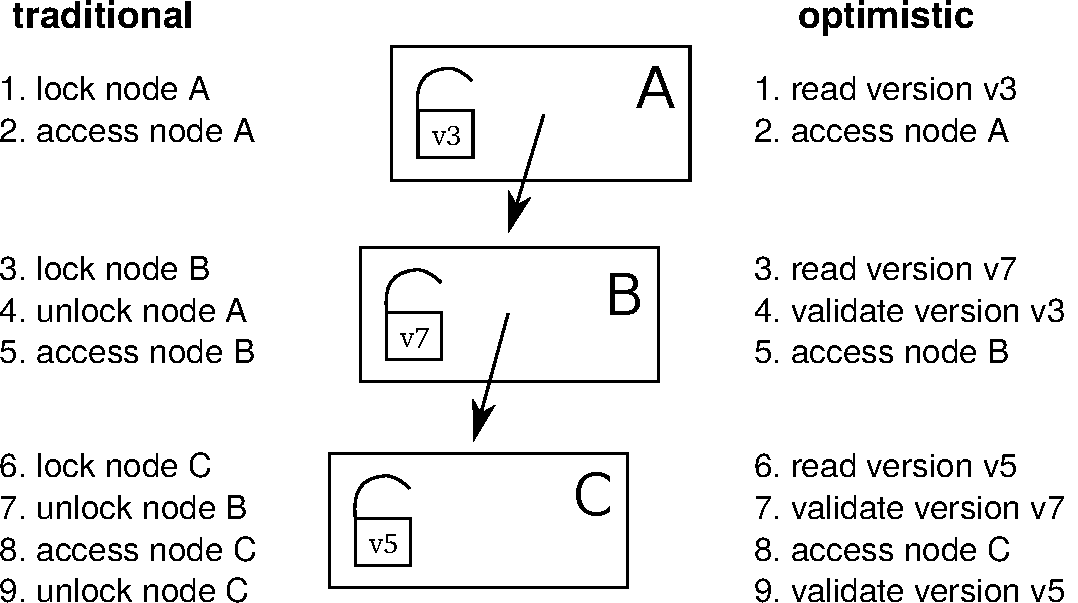
\includegraphics[width=0.65\linewidth]{olcall.pdf}
  \vspace{0.2cm}
  \caption{Comparison of a lookup operation in a 3-level tree using traditional lock coupling (left-hand side) vs.~optimistic lock coupling (right-hand side).}
  \label{fig:olc}
\end{figure}

The traditional and most common lock-based synchronization protocol for B-trees is lock coupling, which interleaves lock acquisitions while holding at most two locks at a time.
If, as we observed earlier, optimistic locks have similar semantics as traditional locks, it is natural to ask whether lock coupling can be combined with optimistic locks.
And indeed the answer is yes: One can almost mechanically translate traditional lock coupling code to optimistic lock coupling code.
This is illustrated in Figure~\ref{fig:olc}, which compares the traversal in a tree of height 3 using traditional and optimistic locks.
As the figure shows, the main difference is that locking is translated to reading the version and that unlocking becomes validation of the previously read version.
This simple change provides efficient lock-free tree traversal without the need to design a complex synchronization protocol.

It is important to emphasize the conceptual simplicity of OLC in comparison to data structures that use custom protocols like the Bw-tree~\cite{DBLP:conf/icde/LevandoskiLS13a}.
To implement lock-free access, the Bw-tree requires an indirection table, delta nodes, complex splitting and merging logic, retry logic, etc.
OLC, on the other hand, can directly be applied to B-trees mostly by adding the appropriate optimistic locking code and without modifying the node layout itself.
Therefore, OpenBw-Tree, an open source implementation of the Bw-tree, requires an order of magnitude more code than a B-tree based on OLC\footnote{Both implementations are available on GitHub: \url{https://github.com/wangziqi2016/index-microbench}}.
Given how difficult it is to develop, validate, and debug lock-free code, simplicity is obviously a major advantage.

\subsection{Correctness Aspects}

\begin{figure}
  % \centering
  %[basicstyle=\normalsize\ttfamily,showstringspaces=false,columns=fullflexible,breaklines=false,breakatwhitespace=true,numbers=none,numberstyle=\small,style=C,keepspaces=true]
\begin{lstlisting}[basicstyle=\ttfamily,language=C++,numbers=left,numberstyle=\small]
std::atomic<BTreeNode*> root;

// search for key in B+tree, returns payload in resultOut
bool lookup(Key key, Value& resultOut) {
   BTreeNode* node = root.load();
   uint64_t nodeVersion = node->readLockOrRestart();
   if (node != root.load()) // make sure the root is still the root
      restart();

   BTreeInner<Key>* parent = nullptr;
   uint64_t parentVersion = 0;

   while (node->isInner()) {
      auto inner = (BTreeInner*)node;

      // unlock parent and make current node the parent
      if (parent)
         parent->readUnlockOrRestart(parentVersion);
      parent = inner;
      parentVersion = nodeVersion;

      // search for next node
      node = inner->findChild(key);
      // validate 'inner' to ensure that 'node' pointer is valid
      inner->checkOrRestart(nodeVersion);
      // now it safe to dereference 'node' pointer (read its version)
      nodeVersion = node->readLockOrRestart();
   }

   // search in leaf and retrieve payload
   auto leaf = (BTreeLeaf*)node;
   bool success = leaf->findValue(key, resultOut);

   // unlock everything
   if (parent)
      parent->readUnlockOrRestart(parentVersion);
   node->readUnlockOrRestart(nodeVersion);

   return success;
}
\end{lstlisting}
  \vspace{0.2cm}
  \caption{B-tree lookup code using OLC. For simplicity, the restart logic is not shown.}
  \label{fig:lookup}
\end{figure}

So far, we have introduced the high-level ideas behind OLC and have stressed its similarity to traditional lock coupling.
Let us now discuss some cases where the close similarity between lock coupling and OLC breaks down.
To make this more concrete, we show the B-tree lookup code in Figure~\ref{fig:lookup}.
In the code, \texttt{readLockOrRestart} reads the lock version and \texttt{readUnlockOrRestart} validates that the read was correct.

One issue with OLC is that any pointer speculatively read from a node may point to invalid memory (if that node is modified concurrently).
Dereferencing such a pointer (e.g., to read its optimistic lock), may cause a segmentation fault or undefined behavior.
In the code shown in Figure~\ref{fig:lookup}, this problem is prevented by the extra check in line 25, which ensures that the read from the node containing the pointer was correct.
Without this additional validation, the code would in line 27 dereference the pointer speculatively read in line 23.
Note that the implementation of \texttt{checkOrRestart} is actually identical to \texttt{readUnlockOrRestart}.
We chose to give it a different name to highlight the fact that this extra check would not be necessary with read/write locks.

Another potential issue with optimistic locks is code that does not terminate.
Code that speculatively accesses a node, like an intra-node binary search, should be written in a way such that it always terminates---even in the presence of concurrent writes.
Otherwise, the validation code that detects the concurrent write will never run.
The binary search of a B-tree, for example, needs to be written in such a way that each comparison makes progress.
For some data structures that do not require loops in the traversal code (like ART) termination is trivially true.

\subsection{Implementation Details}

% implementation, efficiency
To implement an optimistic lock, one can combine the lock and the version counter into a single 64-bit\footnote{Even after subtracting one bit for the lock status, a back-of-the-envelope calculation can show that 63 bits are large enough to never overflow in practice.} word~\cite{artsync}.
A typical read operation will therefore merely consist of reading this version counter atomically.
In C++11 this can be implemented using the \texttt{std::atomic} type.

On x86, atomic reads are cheap because of x86's strong memory order guarantees.
No memory fences are required for sequentially-consistent loads, which are translated (by both GCC and clang) into standard \texttt{MOV} instructions.
Hence, the only effect of \texttt{std::atomic} for loads is preventing instruction re-ordering.
This makes version access and validation cheap.
Acquiring and releasing an optimistic lock in exclusive mode has comparable cost to a traditional lock:
A fairly expensive sequentially-consistent store is needed for acquiring a lock, while a standard \texttt{MOV} suffices for releasing it.
A simple sinlock-based implementation of optimistic locks can be found in the appendix of an earlier paper~\cite{artsync}.

OLC code must be able to handle restarts since validation or lock upgrade can fail due to concurrent writers.
Restarts can easily be implemented by wrapping the data structure operation in a loop (for simplicity not shown in Figure~\ref{fig:lookup}).
Such a loop also enables limiting the number of optimistic retry operations and falling back to pessimistic locking in cases of very heavy contention.
The ability to fall back to traditional locking is a major advantage of OLC in terms of robustness over lock-free approaches, which do not have this option.

In addition to the optimistic shared mode and the exclusive mode, optimistic locks also support a ``shared pessimistic'' mode, which physically acquires the lock in shared mode (allowing multiple concurrent readers but no writers).
This mode is useful for table (or range) scans that touch many tuples on a leaf page (which would otherwise easily abort).
Finally, let us mention that large range scans and table scans, should be broken up into several per-node traversals as is done in the LeanStore~\cite{leanstore} system.

Like all lock-free data structures, but unlike traditional locking and Hardware Transactional Memory~\cite{DBLP:conf/hpca/KarnagelDRLLSL14,DBLP:journals/pvldb/MakreshanskiLS15,htmtkde}, OLC requires care when deleting (and reusing) nodes.
The reason is that a deleting thread can never be sure that a node can be reclaimed because other threads might still be optimistically reading from that node.
Therefore, standard solutions like epoch-based reclamation~\cite{DBLP:conf/sosp/TuZKLM13}, hazard pointers~\cite{DBLP:journals/tpds/Michael04}, or optimized hazard pointers~\cite{DBLP:conf/spaa/BalmauGHZ16} need to be used.
These memory reclamation techniques are, however, largely orthogonal to the synchronization protocol itself.

%-lock-free is not a strong guarantee

\newpage
\section{Evaluation}\label{sec:evaluation}

Let us now experimentally evaluate the overhead and scalability of OLC.
For the experiments, we use an in-memory B+tree implemented in C++11 using templates, which is configured to use nodes of 4096 bytes, random 8 byte keys, and 8 byte payloads.
Based on this B-tree, we compare the following synchronization approaches:
\begin{itemize}
\item an OLC implementation\footnote{An almost identical OLC implementation is available on github: \url{https://github.com/wangziqi2016/index-microbench/tree/master/BTreeOLC}}
\item a variant based on traditional lock coupling and read/write locks
\item the unsynchronized B-tree, which obviously is only correct for read-only workloads but allows measuring the overhead of synchronization
\end{itemize}
Note that earlier work has compared the OLC implementation with a Bw-tree implementation~\cite{buzzword} and other state-of-the-art in-memory index structures.

We use a Haswell EP system with an Intel Xeon E5-2687W v3 CPU, which has 10 cores (20 ``Hyper-Threads'') and 25~MB of L3 cache.
The system is running Ubuntu 18.10 and we use GCC 8.2.0 to compile our code.
The CPU counters are obtained using the Linux perf API\footnote{We use the following convenience wrapper: \url{https://github.com/viktorleis/perfevent}}.

\begin{table}
  \caption{Performance and CPU counters for lookup and insert operations in a B-tree with 100M keys. We perform 100M operations and normalize the CPU counters by that number.}
  \label{tab:overhead}
  \centering
  \begin{tabular}{lrrrrrrr}\toprule
                    &         &        &        & instruc-  & L1     & L3     & branch \\
                    & threads & M op/s & cycles & tions & misses & misses & misses \\\midrule
lookup (no sync.)   & 1       & 1.72   & 2028   & 283     & 39.1   & 14.9   & 16.1   \\
lookup (OLC)        & 1       & 1.65   & 2107   & 370     & 43.9   & 15.1   & 16.7   \\
lookup (lock coup.) & 1       & 1.72   & 2078   & 365     & 42.3   & 16.9   & 15.7   \\\midrule
insert (no sync.)   & 1       & 1.51   & 2286   & 530     & 59.8   & 31.1   & 17.3   \\
insert (OLC)        & 1       & 1.50   & 2303   & 629     & 61.2   & 31.1   & 16.5   \\
insert (lock coup.) & 1       & 1.41   & 2473   & 644     & 61.0   & 31.0   & 17.2   \\\midrule
lookup (no sync.)   & 10      & 15.48  & 2058   & 283     & 38.6   & 15.5   & 16.0   \\
lookup (OLC)        & 10      & 14.60  & 2187   & 370     & 43.8   & 15.8   & 16.8   \\
lookup (lock coup.) & 10      & 5.71   & 5591   & 379     & 54.2   & 17.0   & 14.8   \\\midrule
insert (no sync.)   & 10      & -      & -      & -       & -      & -      & -      \\
insert (OLC)        & 10      & 10.46  & 2940   & 656     & 62.0   & 32.5   & 16.8   \\
insert (lock coup.) & 10      & 7.55   & 4161   & 667     & 75.0   & 28.6   & 16.2   \\
    \bottomrule
\end{tabular}
\end{table}

Table~\ref{tab:overhead} compares the performance and CPU counters for lookup and insert operations in a B-tree with 100M keys.
With {\em single-threaded} execution, we observe that all three approaches have very similar performance.
Adding traditional or optimistic locks to unsynchronized B-tree code results in up to 30\% of additional instructions without affecting single-threaded performance much.

\begin{figure}
  \centering
  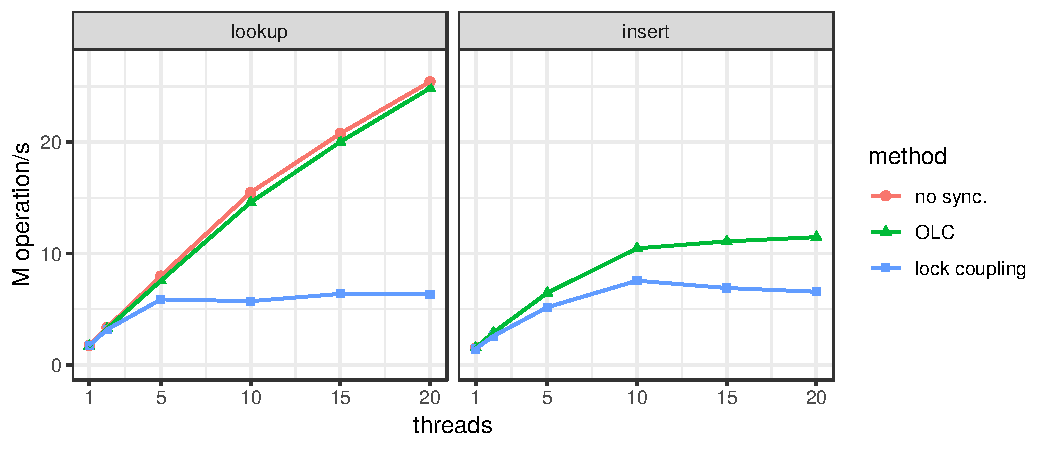
\includegraphics[width=\linewidth]{scale.pdf}
  \vspace{0.2cm}
  \caption{Scalability on 10-core system for B-tree operations (100M values).}
  \label{fig:scale}
\end{figure}

As Figure~\ref{fig:scale} shows, the results change dramatically once we use multiple threads.
For lookup, the scalability of OLC is near-linear up to 20 threads, even though the system has only 10 ``real cores''.
The OLC scalability for insert is also respectable (though not quite as linear because multi-threaded insertion approaches the memory bandwidth of our processor).
The figure also shows that the results of traditional lock coupling with read/write locks are significantly worse than OLC.
With 20 threads, lookup with OLC is 3.9$\times$ faster than traditional lock coupling.

\section{Summary}\label{sec:conc}

Optimistic Lock Coupling (OLC) is an effective synchronization method that combines the simplicity of traditional lock coupling with the superior scalability of lock-free approaches.
OLC is widely applicable and has already been successfully used to synchronize several data structures, including B-trees, binary search trees, and different trie variants.
These features make it highly attractive for modern database systems as well as performance-critical systems software in general.

\begin{thebibliography}{10}

\bibitem{DBLP:conf/spaa/BalmauGHZ16}
O.~Balmau, R.~Guerraoui, M.~Herlihy, and I.~Zablotchi.
\newblock Fast and robust memory reclamation for concurrent data structures.
\newblock In {\em SPAA}, 2016.

\bibitem{DBLP:journals/acta/BayerS77}
R.~Bayer and M.~Schkolnick.
\newblock Concurrency of operations on {B}-trees.
\newblock {\em Acta Informatica}, 9, 1977.

\bibitem{hot}
R.~Binna, E.~Zangerle, M.~Pichl, G.~Specht, and V.~Leis.
\newblock {HOT}: A height optimized trie index for main-memory database
  systems.
\newblock In {\em SIGMOD}, 2018.

\bibitem{DBLP:conf/ppopp/BronsonCCO10}
N.~G. Bronson, J.~Casper, H.~Chafi, and K.~Olukotun.
\newblock A practical concurrent binary search tree.
\newblock In {\em PPOPP}, 2010.

\bibitem{DBLP:conf/vldb/ChaHKK01}
S.~K. Cha, S.~Hwang, K.~Kim, and K.~Kwon.
\newblock Cache-conscious concurrency control of main-memory indexes on
  shared-memory multiprocessor systems.
\newblock In {\em VLDB}, 2001.

\bibitem{intel}
I.~Cutress.
\newblock {Intel} goes for 48-cores: {Cascade-AP} with multi-chip package
  coming soon.
\newblock
  \url{https://www.anandtech.com/show/13535/intel-goes-for-48cores-cascade-ap},
  2018 (accessed January, 2019).

\bibitem{DBLP:conf/cidr/FaleiroA17}
J.~M. Faleiro and D.~J. Abadi.
\newblock Latch-free synchronization in database systems: Silver bullet or
  fool's gold?
\newblock In {\em CIDR}, 2017.

\bibitem{DBLP:journals/ftdb/Graefe11}
G.~Graefe.
\newblock Modern {B}-tree techniques.
\newblock {\em Foundations and Trends in Databases}, 3(4), 2011.

\bibitem{DBLP:conf/hpca/KarnagelDRLLSL14}
T.~Karnagel, R.~Dementiev, R.~Rajwar, K.~Lai, T.~Legler, B.~Schlegel, and
  W.~Lehner.
\newblock Improving in-memory database index performance with
  {Intel}\({}^{\mbox{{\textregistered}}}\) transactional synchronization
  extensions.
\newblock In {\em HPCA}, 2014.

\bibitem{DBLP:journals/tods/LehmanY81}
P.~L. Lehman and S.~B. Yao.
\newblock Efficient locking for concurrent operations on {B}-trees.
\newblock {\em {ACM} Trans. Database Syst.}, 6(4), 1981.

\bibitem{leanstore}
V.~Leis, M.~Haubenschild, A.~Kemper, and T.~Neumann.
\newblock Leanstore: In-memory data management beyond main memory.
\newblock In {\em ICDE}, 2018.

\bibitem{art}
V.~Leis, A.~Kemper, and T.~Neumann.
\newblock The adaptive radix tree: {ARTful} indexing for main-memory databases.
\newblock In {\em ICDE}, 2013.

\bibitem{htmtkde}
V.~Leis, A.~Kemper, and T.~Neumann.
\newblock Scaling {HTM}-supported database transactions to many cores.
\newblock {\em {IEEE} Trans. Knowl. Data Eng.}, 28(2), 2016.

\bibitem{artsync}
V.~Leis, F.~Scheibner, A.~Kemper, and T.~Neumann.
\newblock The {ART} of practical synchronization.
\newblock In {\em DaMoN}, 2016.

\bibitem{DBLP:conf/icde/LevandoskiLS13a}
J.~J. Levandoski, D.~B. Lomet, and S.~Sengupta.
\newblock The {Bw}-tree: A {B}-tree for new hardware platforms.
\newblock In {\em ICDE}, 2013.

\bibitem{DBLP:journals/pvldb/MakreshanskiLS15}
D.~Makreshanski, J.~J. Levandoski, and R.~Stutsman.
\newblock To lock, swap, or elide: On the interplay of hardware transactional
  memory and lock-free indexing.
\newblock {\em {PVLDB}}, 8(11), 2015.

\bibitem{DBLP:dblp_conf/eurosys/MaoKM12}
Y.~Mao, E.~Kohler, and R.~T. Morris.
\newblock Cache craftiness for fast multicore key-value storage.
\newblock In {\em EuroSys}, 2012.

\bibitem{DBLP:journals/tpds/Michael04}
M.~M. Michael.
\newblock Hazard pointers: Safe memory reclamation for lock-free objects.
\newblock {\em {IEEE} Trans. Parallel Distrib. Syst.}, 15(6), 2004.

\bibitem{DBLP:journals/jacm/ShalevS06}
O.~Shalev and N.~Shavit.
\newblock Split-ordered lists: Lock-free extensible hash tables.
\newblock {\em J. {ACM}}, 53(3), 2006.

\bibitem{amd}
A.~Shilov.
\newblock {AMD} previews {EPYC} ‘{Rome}’ processor: Up to 64 {Zen} 2 cores.
\newblock
  \url{https://www.anandtech.com/show/13561/amd-previews-epyc-rome-processor-up-to-64-zen-2-cores},
  2018 (accessed January, 2019).

\bibitem{DBLP:conf/sosp/TuZKLM13}
S.~Tu, W.~Zheng, E.~Kohler, B.~Liskov, and S.~Madden.
\newblock Speedy transactions in multicore in-memory databases.
\newblock In {\em SOSP}, 2013.

\bibitem{buzzword}
Z.~Wang, A.~Pavlo, H.~Lim, V.~Leis, H.~Zhang, M.~Kaminsky, and D.~Andersen.
\newblock Building a {Bw}-tree takes more than just buzz words.
\newblock In {\em SIGMOD}, 2018.

\end{thebibliography}


%\bibliographystyle{abbrv}
%\bibliography{main}

\end{document}

\end{article}


\begin{article}
{Federated Learning without Full Labels: A Survey}
{Yilun Jin, Yang Liu, Kai Chen, and Qiang Yang}
\pdfminorversion=5
\documentclass[11pt]{article}
\usepackage{deauthor,times,graphicx,caption,microtype}
\usepackage{hyperref}
\usepackage{listings}
\usepackage{booktabs}

\begin{document}

\title{Optimistic Lock Coupling: A Scalable and Efficient General-Purpose Synchronization Method}

\author{Viktor Leis, Michael Haubenschild\raisebox{0.9ex}{$\ast$}, Thomas Neumann\\ Technische Universit{\"a}t M{\"u}nchen \hspace{0.7cm} Tableau Software\raisebox{0.9ex}{$\ast$} \\ {\{leis,neumann\}{@}in.tum.de} \hspace{0.7cm} {mhaubenschild{@}tableau.com\raisebox{0.9ex}{$\ast$}}}

\maketitle

\begin{abstract}
As the number of cores on commodity processors continues to increase, scalability becomes more and more crucial for overall performance.
Scalable and efficient concurrent data structures are particularly important, as these are often the building blocks of parallel algorithms.
Unfortunately, traditional synchronization techniques based on fine-grained locking have been shown to be unscalable on modern multi-core CPUs.
Lock-free data structures, on the other hand, are extremely difficult to design and often incur significant overhead.

In this work, we make the case for Optimistic Lock Coupling as a practical alternative to both traditional locking and the lock-free approach.
We show that Optimistic Lock Coupling is highly scalable and almost as simple to implement as traditional lock coupling.
Another important advantage is that it is easily applicable to most tree-like data structures.
We therefore argue that Optimistic Lock Coupling, rather than a complex and error-prone custom synchronization protocol, should be the default choice for performance-critical data structures.
\end{abstract}

\section{Introduction}

% more and more cores
Today, Intel's commodity server processors have up to 28 cores and its upcoming microarchitecture will have up to 48 cores per socket~\cite{intel}.
Similarly, AMD currently stands at 32 cores and this number is expected to double in the next generation~\cite{amd}.
Since both platforms support simultaneous multithreading (also known as hyperthreading), affordable commodity servers (with up to two sockets) will soon routinely have between 100 and 200 hardware threads.

% data structure scalability is important
With such a high degree of hardware parallelism, efficient data processing crucially depends on how well concurrent data structures scale.
Internally, database systems use a plethora of data structures like table heaps, internal work queues, and, most importantly, index structures.
Any of these can easily become a scalability (and therefore overall performance) bottleneck on many-core CPUs.

% traditional synchronization: fine-grained locks, slow, cache invalidation
Traditionally, database systems synchronize internal data structures using fine-grained reader/writer locks\footnote{In this work, we focus on data structure synchronization rather than high-level transaction semantics and therefore use the term {\em lock} for what would typically be called {\em latch} in the database literature. We thus follow common computer science (rather than database) terminology.}.
Unfortunately, while fine-grained locking makes lock contention unlikely, it still results in bad scalability because lock acquisition and release require writing to shared memory.
Due to the way cache coherency is implemented on modern multi-core CPUs, these writes cause additional cache misses\footnote{The cache coherency protocol ensures that all copies of a cache line on other cores are invalidated before the write can proceed.} and the cache line containing the lock's internal data becomes a point of physical contention.
As a result, any frequently-accessed lock (e.g., the lock of the root node of a B-tree) severely limits scalability.

% lock-free bw-tree: no more latches, but indirections, extremely complex
Lock-free data structures like the Bw-tree~\cite{DBLP:conf/icde/LevandoskiLS13a} (a lock-free B-tree variant) or the Split-Ordered List~\cite{DBLP:journals/jacm/ShalevS06} (a lock-free hash table) do not acquire any locks and therefore generally scale much better than locking-based approaches (in particular for read-mostly workloads).
However, lock-free synchronization has other downsides:
First, it is very difficult and results in extremely complex and error-prone code (when compared to locking).
Second, because the functionality of atomic primitives provided by the hardware (e.g., atomically compare-and-swap 8 bytes) is limited, complex operations require additional indirections within the data structure.
For example, the Bw-tree requires an indirection table and the Split-Ordered List requires ``dummy nodes'', resulting in overhead due to additional cache misses.

% OLC for the win
In this paper we make the case for {\em Optimistic Lock Coupling (OLC)}, a synchronization method that combines some of the best properties of lock-based and lock-free synchronization.
OLC utilizes a special lock type that can be used in two modes:
The first mode is similar to a traditional mutex and excludes other threads by physically acquiring the underlying lock.
In the second mode, reads can proceed optimistically by validating a version counter that is embedded in the lock (similar to optimistic concurrency control).
The first mode is typically used by writers and the second mode by readers.
Besides this special lock type, OLC is based on the observation that optimistic lock validations can be interleaved/coupled---similar to the pair-wise interleaved lock acquisition of traditional lock coupling.
Hence, the name Optimistic Lock Coupling.

OLC has a number of desirable features:
\begin{itemize}
\item By reducing the number of writes to shared memory locations and thereby avoiding cache invalidations, it {\bf scales well} for most workloads.
\item In comparison to unsynchronized code, it requires few additional CPU instructions making it {\bf efficient}.
\item OLC is {\bf widely applicable} to different data structures. It has already been successfully used for synchronizing binary search trees~\cite{DBLP:conf/ppopp/BronsonCCO10}, tries~\cite{artsync}, trie/B-tree hybrids~\cite{DBLP:dblp_conf/eurosys/MaoKM12}, and B-trees~\cite{buzzword}.
\item In comparison to the lock-free paradigm, it is also {\bf easy to use} and requires few modifications to existing, single-threaded data structures.
\end{itemize}
Despite these positive features and its simplicity, OLC is not yet widely known.
The goal of this paper is therefore to popularize this simple idea and to make a case for it.
We argue that OLC deserves to be widely known.
It is a good default synchronization paradigm---more complex, data structure-specific protocols are seldom beneficial.

The rest of the paper is organized as follows.
Section~\ref{sec:related} discusses related work, tracing the history of OLC and its underlying ideas in the literature.
The core of the paper is Section~\ref{sec:olc}, which describes the ideas behind OLC and how it can be used to synchronize complex data structures.
In Section~\ref{sec:evaluation} we experimentally show that OLC has low overhead and scales well when used to synchronize an in-memory B-tree.
We summarize the paper in Section~\ref{sec:conc}.

\newpage
\section{Related Work}\label{sec:related}

Lock coupling has been proposed as a method for allowing concurrent operations on B-trees in 1977~\cite{DBLP:journals/acta/BayerS77}.
This traditional and still widely-used method, described in detail in Graefe's B-tree survey~\cite{DBLP:journals/ftdb/Graefe11}, is also called ``latch coupling'', ``hand-over-hand locking'', and ``crabbing''.
Because at most two locks are held at-a-time during tree traversal, this technique seemingly allows for a high degree of parallelism---in particular if read/write locks are used to enable inner nodes to be locked in shared mode.
However, as we show in Section~\ref{sec:evaluation}, on modern hardware lock acquisition (even in shared mode) results in suboptimal scalability.

An early alternative from 1981 is a B-tree variant called B-link tree~\cite{DBLP:journals/tods/LehmanY81}, which only holds a single lock at a time.
It is based on the observation that between the release of the parent lock and the acquisition of the child lock, the only ``dangerous'' thing that could have happened is the split of a child node (assuming one does not implement merge operations).
Thus, when a split happens, the key being searched might end up on a neighboring node to the right of the current child node.
A B-link tree traversal therefore detects this condition and, if needed, transparently proceeds to the neighboring node.
Releasing the parent lock early is highly beneficial when the child node needs to be fetched from disk.
For in-memory workloads, however, the B-link tree has the same scalability issues as lock coupling (it acquires just as many locks).

The next major advance, Optimistic Latch-Free Index Traversal (OLFIT)~\cite{DBLP:conf/vldb/ChaHKK01}, was proposed in 2001.
OLFIT introduced the idea of a combined lock/update counter, which we call {\em optimistic lock}. % , for lack of a better name,
Based on these per-node optimistic locks and the synchronization protocol of the B-link tree, OLFIT finally achieves good scalability on parallel processors.
The OLFIT protocol is fairly complex, as it requires both the non-trivial B-link protocol and optimistic locks.
Furthermore, like the B-link tree protocol, it does not support merging nodes, and is specific to B-trees (cannot easily be applied to other data structures).

In the following two decades, the growth of main-memory capacity led to much research into other data structures besides the venerable B-tree.
Particularly relevant for our discussion is Bronson et al.'s~\cite{DBLP:conf/ppopp/BronsonCCO10} concurrent binary search tree, which is based on optimistic version validation and has a sophisticated, data structure-specific synchronization protocol.
To the best of our knowledge, this 2010 paper is the first that, as part of its protocol, interleaves version validation across nodes---rather than validating each node separately like OLFIT.
In that paper, this idea is called ``hand-over-hand, optimistic validation'', while we prefer the term Optimistic Lock Coupling to highlight the close resemblance to traditional lock coupling.
Similarly, Mao et al.'s~\cite{DBLP:dblp_conf/eurosys/MaoKM12} Masstree (a concurrent hybrid trie/B-tree) is also based on the same ideas, but again uses them as part of a more complex protocol.

The Adaptive Radix Tree (ART)~\cite{art} is another recent in-memory data structure, which we proposed in 2013.
In contrast to the two data structures just mentioned, it was originally designed with single-threaded performance in mind without supporting concurrency.
To add support for concurrency, we initially started designing a custom protocol called Read-Optimized Write Exclusion (ROWEX)~\cite{artsync}, which turned out to be non-trivial and requires modifications of the underlying data structure\footnote{Note that ROWEX is already easier to apply to existing data structures than the lock-free approach. The difficulty depends on the data structure. Applying ROWEX is hard for B-trees with sorted keys and fairly easy for copy-on-write data structures like the Height Optimized Trie~\cite{hot}---with ART being somewhere in the middle.}.
However, fairly late in the project, we also realized, that OLC {\em alone} (rather than as part of a more complex protocol) is sufficient to synchronize ART.
No other changes to the data structure were necessary.
Both approaches were published and experimentally evaluated in a followup paper~\cite{artsync}, which shows that, despite its simplicity, OLC is efficient, scalable, and generally outperforms ROWEX.

Similar results were recently published regarding B-trees~\cite{buzzword}.
In this experimental study a simple OLC-based synchronization outperformed the Bw-tree~\cite{DBLP:conf/icde/LevandoskiLS13a}, a complex lock-free synchronization approach.
Another recent paper shows that for write-intensive workloads, locking often performs better than lock-free synchronization~\cite{DBLP:conf/cidr/FaleiroA17}.
These experiences indicate that OLC is a general-purpose synchronization paradigm and motivate the current paper.

%foster b-tree\cite{DBLP:journals/tods/GraefeKK12}
%Shasha theory~\cite{DBLP:journals/tods/ShashaG88}

\section{Optimistic Lock Coupling}\label{sec:olc}

% locks suck
The standard technique for inter-thread synchronization is mutual exclusion using fine-grained locks.
In a B-tree, for example, every node usually has its own associated lock, which is acquired before accessing that node.
The problem of locking on modern multi- and many-core processors is that lock acquisition and release require writing to the shared memory location that implements the lock.
This write causes exclusive ownership of the underlying cache line and invalidates copies of it on all other processor cores.
For hierarchical, tree-like data structures, the lock of the root node becomes a point of physical contention---even in read-only workloads and even when read/write locks are used.
Depending on the specific data structure, number of cores, cache coherency protocol implementation, cache topology, whether Non-Uniform Memory Access (NUMA) is used, locking can even result in multi-threaded performance that is worse than single-threaded execution.

% in b-trees this happens very much
The inherent pessimism of locking is particularly unfortunate for B-trees:
Despite the fact that logical modifications of the root node are very infrequent, every B-tree operation must lock the root node during tree traversal\footnote{To a lesser extent this obviously applies to all inner nodes, not just the root.}.
Even the vast majority of update operations (with the exception of splits and merges), only modify a single leaf node.
These observations indicate that a more optimistic approach, which does not require locking inner nodes, would be very beneficial for B-trees.

\subsection{Optimistic Locks}

% optimism to the rescue
As the name indicates, optimistic locks try to solve the scalability issues of traditional locks using an optimistic approach.
Instead of always physically acquiring locks, even for nodes that are unlikely to be modified simultaneously, after-the-fact validation is used to detect conflicts.
This is done by augmenting each lock with a version/update counter that is incremented on every modification.
Using this version counter, readers can optimistically proceed before validating that the version did not change to ensure that the read was safe.
If validation fails, the operation is restarted.

% details on opt locks
Using optimistic locks, a read-only node access (i.e., the majority of all operations in a B-tree) does not acquire the lock and does not increment the version counter.
Instead, it performs the following steps:
\begin{enumerate}
\item read lock version (restart if lock is not free)
\item access node
\item read the version again and validate that it has not changed in the meantime
\end{enumerate}
If the last step (the validation) fails, the operation has to be restarted.
Write operations, on the other hand, are more similar to traditional locking:
\begin{enumerate}
\item acquire lock (wait if necessary)
\item access/write to node
\item increment version and unlock node
\end{enumerate}
Writes can therefore protect a node from other writes.

% similar to locks
As we observed in an earlier paper~\cite{artsync}, because of similar semantics, optimistic locks can be hidden behind an API very similar to traditional read/write locks.
Both approaches have an exclusive lock mode, and acquiring a traditional lock in shared mode is analogous to optimistic version validation.
Furthermore, like with some implementations of traditional read/write locks, optimistic locks allow upgrading a shared lock to an exclusive lock.
Lock upgrades are, for example, used to avoid most B-tree update operations from having to lock inner nodes.
In our experience, the close resemblance of optimistic and traditional locks simplifies the reasoning about optimistic locks;
one can apply similar thinking as in traditional lock-based protocols.

\subsection{Lock Coupling with Optimistic Locks}

\begin{figure}
  \centering
  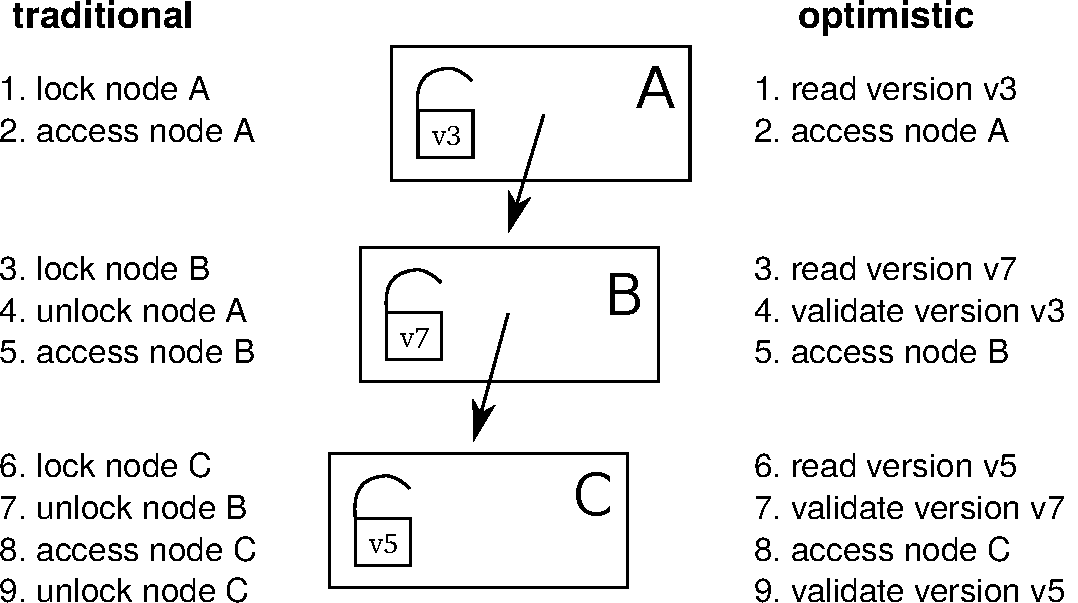
\includegraphics[width=0.65\linewidth]{olcall.pdf}
  \vspace{0.2cm}
  \caption{Comparison of a lookup operation in a 3-level tree using traditional lock coupling (left-hand side) vs.~optimistic lock coupling (right-hand side).}
  \label{fig:olc}
\end{figure}

The traditional and most common lock-based synchronization protocol for B-trees is lock coupling, which interleaves lock acquisitions while holding at most two locks at a time.
If, as we observed earlier, optimistic locks have similar semantics as traditional locks, it is natural to ask whether lock coupling can be combined with optimistic locks.
And indeed the answer is yes: One can almost mechanically translate traditional lock coupling code to optimistic lock coupling code.
This is illustrated in Figure~\ref{fig:olc}, which compares the traversal in a tree of height 3 using traditional and optimistic locks.
As the figure shows, the main difference is that locking is translated to reading the version and that unlocking becomes validation of the previously read version.
This simple change provides efficient lock-free tree traversal without the need to design a complex synchronization protocol.

It is important to emphasize the conceptual simplicity of OLC in comparison to data structures that use custom protocols like the Bw-tree~\cite{DBLP:conf/icde/LevandoskiLS13a}.
To implement lock-free access, the Bw-tree requires an indirection table, delta nodes, complex splitting and merging logic, retry logic, etc.
OLC, on the other hand, can directly be applied to B-trees mostly by adding the appropriate optimistic locking code and without modifying the node layout itself.
Therefore, OpenBw-Tree, an open source implementation of the Bw-tree, requires an order of magnitude more code than a B-tree based on OLC\footnote{Both implementations are available on GitHub: \url{https://github.com/wangziqi2016/index-microbench}}.
Given how difficult it is to develop, validate, and debug lock-free code, simplicity is obviously a major advantage.

\subsection{Correctness Aspects}

\begin{figure}
  % \centering
  %[basicstyle=\normalsize\ttfamily,showstringspaces=false,columns=fullflexible,breaklines=false,breakatwhitespace=true,numbers=none,numberstyle=\small,style=C,keepspaces=true]
\begin{lstlisting}[basicstyle=\ttfamily,language=C++,numbers=left,numberstyle=\small]
std::atomic<BTreeNode*> root;

// search for key in B+tree, returns payload in resultOut
bool lookup(Key key, Value& resultOut) {
   BTreeNode* node = root.load();
   uint64_t nodeVersion = node->readLockOrRestart();
   if (node != root.load()) // make sure the root is still the root
      restart();

   BTreeInner<Key>* parent = nullptr;
   uint64_t parentVersion = 0;

   while (node->isInner()) {
      auto inner = (BTreeInner*)node;

      // unlock parent and make current node the parent
      if (parent)
         parent->readUnlockOrRestart(parentVersion);
      parent = inner;
      parentVersion = nodeVersion;

      // search for next node
      node = inner->findChild(key);
      // validate 'inner' to ensure that 'node' pointer is valid
      inner->checkOrRestart(nodeVersion);
      // now it safe to dereference 'node' pointer (read its version)
      nodeVersion = node->readLockOrRestart();
   }

   // search in leaf and retrieve payload
   auto leaf = (BTreeLeaf*)node;
   bool success = leaf->findValue(key, resultOut);

   // unlock everything
   if (parent)
      parent->readUnlockOrRestart(parentVersion);
   node->readUnlockOrRestart(nodeVersion);

   return success;
}
\end{lstlisting}
  \vspace{0.2cm}
  \caption{B-tree lookup code using OLC. For simplicity, the restart logic is not shown.}
  \label{fig:lookup}
\end{figure}

So far, we have introduced the high-level ideas behind OLC and have stressed its similarity to traditional lock coupling.
Let us now discuss some cases where the close similarity between lock coupling and OLC breaks down.
To make this more concrete, we show the B-tree lookup code in Figure~\ref{fig:lookup}.
In the code, \texttt{readLockOrRestart} reads the lock version and \texttt{readUnlockOrRestart} validates that the read was correct.

One issue with OLC is that any pointer speculatively read from a node may point to invalid memory (if that node is modified concurrently).
Dereferencing such a pointer (e.g., to read its optimistic lock), may cause a segmentation fault or undefined behavior.
In the code shown in Figure~\ref{fig:lookup}, this problem is prevented by the extra check in line 25, which ensures that the read from the node containing the pointer was correct.
Without this additional validation, the code would in line 27 dereference the pointer speculatively read in line 23.
Note that the implementation of \texttt{checkOrRestart} is actually identical to \texttt{readUnlockOrRestart}.
We chose to give it a different name to highlight the fact that this extra check would not be necessary with read/write locks.

Another potential issue with optimistic locks is code that does not terminate.
Code that speculatively accesses a node, like an intra-node binary search, should be written in a way such that it always terminates---even in the presence of concurrent writes.
Otherwise, the validation code that detects the concurrent write will never run.
The binary search of a B-tree, for example, needs to be written in such a way that each comparison makes progress.
For some data structures that do not require loops in the traversal code (like ART) termination is trivially true.

\subsection{Implementation Details}

% implementation, efficiency
To implement an optimistic lock, one can combine the lock and the version counter into a single 64-bit\footnote{Even after subtracting one bit for the lock status, a back-of-the-envelope calculation can show that 63 bits are large enough to never overflow in practice.} word~\cite{artsync}.
A typical read operation will therefore merely consist of reading this version counter atomically.
In C++11 this can be implemented using the \texttt{std::atomic} type.

On x86, atomic reads are cheap because of x86's strong memory order guarantees.
No memory fences are required for sequentially-consistent loads, which are translated (by both GCC and clang) into standard \texttt{MOV} instructions.
Hence, the only effect of \texttt{std::atomic} for loads is preventing instruction re-ordering.
This makes version access and validation cheap.
Acquiring and releasing an optimistic lock in exclusive mode has comparable cost to a traditional lock:
A fairly expensive sequentially-consistent store is needed for acquiring a lock, while a standard \texttt{MOV} suffices for releasing it.
A simple sinlock-based implementation of optimistic locks can be found in the appendix of an earlier paper~\cite{artsync}.

OLC code must be able to handle restarts since validation or lock upgrade can fail due to concurrent writers.
Restarts can easily be implemented by wrapping the data structure operation in a loop (for simplicity not shown in Figure~\ref{fig:lookup}).
Such a loop also enables limiting the number of optimistic retry operations and falling back to pessimistic locking in cases of very heavy contention.
The ability to fall back to traditional locking is a major advantage of OLC in terms of robustness over lock-free approaches, which do not have this option.

In addition to the optimistic shared mode and the exclusive mode, optimistic locks also support a ``shared pessimistic'' mode, which physically acquires the lock in shared mode (allowing multiple concurrent readers but no writers).
This mode is useful for table (or range) scans that touch many tuples on a leaf page (which would otherwise easily abort).
Finally, let us mention that large range scans and table scans, should be broken up into several per-node traversals as is done in the LeanStore~\cite{leanstore} system.

Like all lock-free data structures, but unlike traditional locking and Hardware Transactional Memory~\cite{DBLP:conf/hpca/KarnagelDRLLSL14,DBLP:journals/pvldb/MakreshanskiLS15,htmtkde}, OLC requires care when deleting (and reusing) nodes.
The reason is that a deleting thread can never be sure that a node can be reclaimed because other threads might still be optimistically reading from that node.
Therefore, standard solutions like epoch-based reclamation~\cite{DBLP:conf/sosp/TuZKLM13}, hazard pointers~\cite{DBLP:journals/tpds/Michael04}, or optimized hazard pointers~\cite{DBLP:conf/spaa/BalmauGHZ16} need to be used.
These memory reclamation techniques are, however, largely orthogonal to the synchronization protocol itself.

%-lock-free is not a strong guarantee

\newpage
\section{Evaluation}\label{sec:evaluation}

Let us now experimentally evaluate the overhead and scalability of OLC.
For the experiments, we use an in-memory B+tree implemented in C++11 using templates, which is configured to use nodes of 4096 bytes, random 8 byte keys, and 8 byte payloads.
Based on this B-tree, we compare the following synchronization approaches:
\begin{itemize}
\item an OLC implementation\footnote{An almost identical OLC implementation is available on github: \url{https://github.com/wangziqi2016/index-microbench/tree/master/BTreeOLC}}
\item a variant based on traditional lock coupling and read/write locks
\item the unsynchronized B-tree, which obviously is only correct for read-only workloads but allows measuring the overhead of synchronization
\end{itemize}
Note that earlier work has compared the OLC implementation with a Bw-tree implementation~\cite{buzzword} and other state-of-the-art in-memory index structures.

We use a Haswell EP system with an Intel Xeon E5-2687W v3 CPU, which has 10 cores (20 ``Hyper-Threads'') and 25~MB of L3 cache.
The system is running Ubuntu 18.10 and we use GCC 8.2.0 to compile our code.
The CPU counters are obtained using the Linux perf API\footnote{We use the following convenience wrapper: \url{https://github.com/viktorleis/perfevent}}.

\begin{table}
  \caption{Performance and CPU counters for lookup and insert operations in a B-tree with 100M keys. We perform 100M operations and normalize the CPU counters by that number.}
  \label{tab:overhead}
  \centering
  \begin{tabular}{lrrrrrrr}\toprule
                    &         &        &        & instruc-  & L1     & L3     & branch \\
                    & threads & M op/s & cycles & tions & misses & misses & misses \\\midrule
lookup (no sync.)   & 1       & 1.72   & 2028   & 283     & 39.1   & 14.9   & 16.1   \\
lookup (OLC)        & 1       & 1.65   & 2107   & 370     & 43.9   & 15.1   & 16.7   \\
lookup (lock coup.) & 1       & 1.72   & 2078   & 365     & 42.3   & 16.9   & 15.7   \\\midrule
insert (no sync.)   & 1       & 1.51   & 2286   & 530     & 59.8   & 31.1   & 17.3   \\
insert (OLC)        & 1       & 1.50   & 2303   & 629     & 61.2   & 31.1   & 16.5   \\
insert (lock coup.) & 1       & 1.41   & 2473   & 644     & 61.0   & 31.0   & 17.2   \\\midrule
lookup (no sync.)   & 10      & 15.48  & 2058   & 283     & 38.6   & 15.5   & 16.0   \\
lookup (OLC)        & 10      & 14.60  & 2187   & 370     & 43.8   & 15.8   & 16.8   \\
lookup (lock coup.) & 10      & 5.71   & 5591   & 379     & 54.2   & 17.0   & 14.8   \\\midrule
insert (no sync.)   & 10      & -      & -      & -       & -      & -      & -      \\
insert (OLC)        & 10      & 10.46  & 2940   & 656     & 62.0   & 32.5   & 16.8   \\
insert (lock coup.) & 10      & 7.55   & 4161   & 667     & 75.0   & 28.6   & 16.2   \\
    \bottomrule
\end{tabular}
\end{table}

Table~\ref{tab:overhead} compares the performance and CPU counters for lookup and insert operations in a B-tree with 100M keys.
With {\em single-threaded} execution, we observe that all three approaches have very similar performance.
Adding traditional or optimistic locks to unsynchronized B-tree code results in up to 30\% of additional instructions without affecting single-threaded performance much.

\begin{figure}
  \centering
  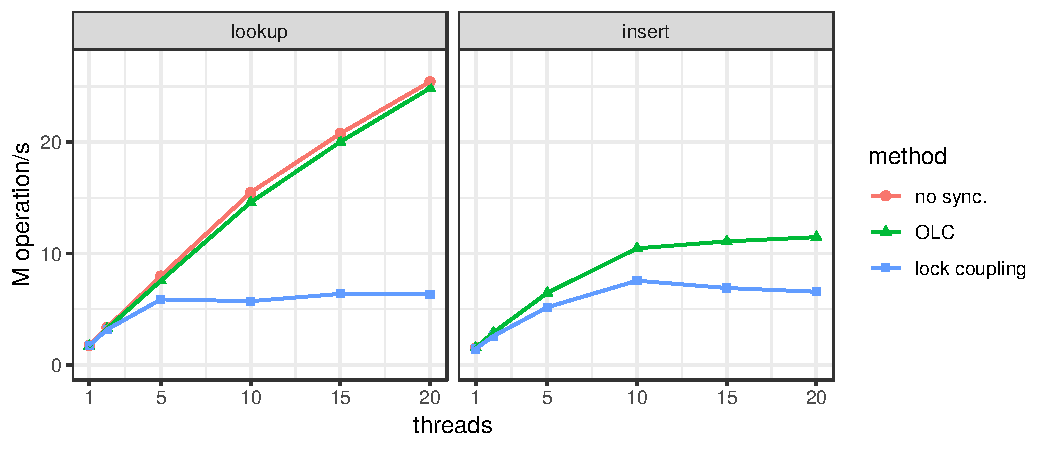
\includegraphics[width=\linewidth]{scale.pdf}
  \vspace{0.2cm}
  \caption{Scalability on 10-core system for B-tree operations (100M values).}
  \label{fig:scale}
\end{figure}

As Figure~\ref{fig:scale} shows, the results change dramatically once we use multiple threads.
For lookup, the scalability of OLC is near-linear up to 20 threads, even though the system has only 10 ``real cores''.
The OLC scalability for insert is also respectable (though not quite as linear because multi-threaded insertion approaches the memory bandwidth of our processor).
The figure also shows that the results of traditional lock coupling with read/write locks are significantly worse than OLC.
With 20 threads, lookup with OLC is 3.9$\times$ faster than traditional lock coupling.

\section{Summary}\label{sec:conc}

Optimistic Lock Coupling (OLC) is an effective synchronization method that combines the simplicity of traditional lock coupling with the superior scalability of lock-free approaches.
OLC is widely applicable and has already been successfully used to synchronize several data structures, including B-trees, binary search trees, and different trie variants.
These features make it highly attractive for modern database systems as well as performance-critical systems software in general.

\begin{thebibliography}{10}

\bibitem{DBLP:conf/spaa/BalmauGHZ16}
O.~Balmau, R.~Guerraoui, M.~Herlihy, and I.~Zablotchi.
\newblock Fast and robust memory reclamation for concurrent data structures.
\newblock In {\em SPAA}, 2016.

\bibitem{DBLP:journals/acta/BayerS77}
R.~Bayer and M.~Schkolnick.
\newblock Concurrency of operations on {B}-trees.
\newblock {\em Acta Informatica}, 9, 1977.

\bibitem{hot}
R.~Binna, E.~Zangerle, M.~Pichl, G.~Specht, and V.~Leis.
\newblock {HOT}: A height optimized trie index for main-memory database
  systems.
\newblock In {\em SIGMOD}, 2018.

\bibitem{DBLP:conf/ppopp/BronsonCCO10}
N.~G. Bronson, J.~Casper, H.~Chafi, and K.~Olukotun.
\newblock A practical concurrent binary search tree.
\newblock In {\em PPOPP}, 2010.

\bibitem{DBLP:conf/vldb/ChaHKK01}
S.~K. Cha, S.~Hwang, K.~Kim, and K.~Kwon.
\newblock Cache-conscious concurrency control of main-memory indexes on
  shared-memory multiprocessor systems.
\newblock In {\em VLDB}, 2001.

\bibitem{intel}
I.~Cutress.
\newblock {Intel} goes for 48-cores: {Cascade-AP} with multi-chip package
  coming soon.
\newblock
  \url{https://www.anandtech.com/show/13535/intel-goes-for-48cores-cascade-ap},
  2018 (accessed January, 2019).

\bibitem{DBLP:conf/cidr/FaleiroA17}
J.~M. Faleiro and D.~J. Abadi.
\newblock Latch-free synchronization in database systems: Silver bullet or
  fool's gold?
\newblock In {\em CIDR}, 2017.

\bibitem{DBLP:journals/ftdb/Graefe11}
G.~Graefe.
\newblock Modern {B}-tree techniques.
\newblock {\em Foundations and Trends in Databases}, 3(4), 2011.

\bibitem{DBLP:conf/hpca/KarnagelDRLLSL14}
T.~Karnagel, R.~Dementiev, R.~Rajwar, K.~Lai, T.~Legler, B.~Schlegel, and
  W.~Lehner.
\newblock Improving in-memory database index performance with
  {Intel}\({}^{\mbox{{\textregistered}}}\) transactional synchronization
  extensions.
\newblock In {\em HPCA}, 2014.

\bibitem{DBLP:journals/tods/LehmanY81}
P.~L. Lehman and S.~B. Yao.
\newblock Efficient locking for concurrent operations on {B}-trees.
\newblock {\em {ACM} Trans. Database Syst.}, 6(4), 1981.

\bibitem{leanstore}
V.~Leis, M.~Haubenschild, A.~Kemper, and T.~Neumann.
\newblock Leanstore: In-memory data management beyond main memory.
\newblock In {\em ICDE}, 2018.

\bibitem{art}
V.~Leis, A.~Kemper, and T.~Neumann.
\newblock The adaptive radix tree: {ARTful} indexing for main-memory databases.
\newblock In {\em ICDE}, 2013.

\bibitem{htmtkde}
V.~Leis, A.~Kemper, and T.~Neumann.
\newblock Scaling {HTM}-supported database transactions to many cores.
\newblock {\em {IEEE} Trans. Knowl. Data Eng.}, 28(2), 2016.

\bibitem{artsync}
V.~Leis, F.~Scheibner, A.~Kemper, and T.~Neumann.
\newblock The {ART} of practical synchronization.
\newblock In {\em DaMoN}, 2016.

\bibitem{DBLP:conf/icde/LevandoskiLS13a}
J.~J. Levandoski, D.~B. Lomet, and S.~Sengupta.
\newblock The {Bw}-tree: A {B}-tree for new hardware platforms.
\newblock In {\em ICDE}, 2013.

\bibitem{DBLP:journals/pvldb/MakreshanskiLS15}
D.~Makreshanski, J.~J. Levandoski, and R.~Stutsman.
\newblock To lock, swap, or elide: On the interplay of hardware transactional
  memory and lock-free indexing.
\newblock {\em {PVLDB}}, 8(11), 2015.

\bibitem{DBLP:dblp_conf/eurosys/MaoKM12}
Y.~Mao, E.~Kohler, and R.~T. Morris.
\newblock Cache craftiness for fast multicore key-value storage.
\newblock In {\em EuroSys}, 2012.

\bibitem{DBLP:journals/tpds/Michael04}
M.~M. Michael.
\newblock Hazard pointers: Safe memory reclamation for lock-free objects.
\newblock {\em {IEEE} Trans. Parallel Distrib. Syst.}, 15(6), 2004.

\bibitem{DBLP:journals/jacm/ShalevS06}
O.~Shalev and N.~Shavit.
\newblock Split-ordered lists: Lock-free extensible hash tables.
\newblock {\em J. {ACM}}, 53(3), 2006.

\bibitem{amd}
A.~Shilov.
\newblock {AMD} previews {EPYC} ‘{Rome}’ processor: Up to 64 {Zen} 2 cores.
\newblock
  \url{https://www.anandtech.com/show/13561/amd-previews-epyc-rome-processor-up-to-64-zen-2-cores},
  2018 (accessed January, 2019).

\bibitem{DBLP:conf/sosp/TuZKLM13}
S.~Tu, W.~Zheng, E.~Kohler, B.~Liskov, and S.~Madden.
\newblock Speedy transactions in multicore in-memory databases.
\newblock In {\em SOSP}, 2013.

\bibitem{buzzword}
Z.~Wang, A.~Pavlo, H.~Lim, V.~Leis, H.~Zhang, M.~Kaminsky, and D.~Andersen.
\newblock Building a {Bw}-tree takes more than just buzz words.
\newblock In {\em SIGMOD}, 2018.

\end{thebibliography}


%\bibliographystyle{abbrv}
%\bibliography{main}

\end{document}

\end{article}

\begin{article}
{Federated Computing: Query, Learning, and Beyond}
{Yongxin Tong, Yuxiang Zeng, Zimu Zhou, Boyi Liu, Yexuan Shi, Shuyuan Li, Ke Xu,and Weifeng Lv}
\pdfminorversion=5
\documentclass[11pt]{article}
\usepackage{deauthor,times,graphicx,caption,microtype}
\usepackage{hyperref}
\usepackage{listings}
\usepackage{booktabs}

\begin{document}

\title{Optimistic Lock Coupling: A Scalable and Efficient General-Purpose Synchronization Method}

\author{Viktor Leis, Michael Haubenschild\raisebox{0.9ex}{$\ast$}, Thomas Neumann\\ Technische Universit{\"a}t M{\"u}nchen \hspace{0.7cm} Tableau Software\raisebox{0.9ex}{$\ast$} \\ {\{leis,neumann\}{@}in.tum.de} \hspace{0.7cm} {mhaubenschild{@}tableau.com\raisebox{0.9ex}{$\ast$}}}

\maketitle

\begin{abstract}
As the number of cores on commodity processors continues to increase, scalability becomes more and more crucial for overall performance.
Scalable and efficient concurrent data structures are particularly important, as these are often the building blocks of parallel algorithms.
Unfortunately, traditional synchronization techniques based on fine-grained locking have been shown to be unscalable on modern multi-core CPUs.
Lock-free data structures, on the other hand, are extremely difficult to design and often incur significant overhead.

In this work, we make the case for Optimistic Lock Coupling as a practical alternative to both traditional locking and the lock-free approach.
We show that Optimistic Lock Coupling is highly scalable and almost as simple to implement as traditional lock coupling.
Another important advantage is that it is easily applicable to most tree-like data structures.
We therefore argue that Optimistic Lock Coupling, rather than a complex and error-prone custom synchronization protocol, should be the default choice for performance-critical data structures.
\end{abstract}

\section{Introduction}

% more and more cores
Today, Intel's commodity server processors have up to 28 cores and its upcoming microarchitecture will have up to 48 cores per socket~\cite{intel}.
Similarly, AMD currently stands at 32 cores and this number is expected to double in the next generation~\cite{amd}.
Since both platforms support simultaneous multithreading (also known as hyperthreading), affordable commodity servers (with up to two sockets) will soon routinely have between 100 and 200 hardware threads.

% data structure scalability is important
With such a high degree of hardware parallelism, efficient data processing crucially depends on how well concurrent data structures scale.
Internally, database systems use a plethora of data structures like table heaps, internal work queues, and, most importantly, index structures.
Any of these can easily become a scalability (and therefore overall performance) bottleneck on many-core CPUs.

% traditional synchronization: fine-grained locks, slow, cache invalidation
Traditionally, database systems synchronize internal data structures using fine-grained reader/writer locks\footnote{In this work, we focus on data structure synchronization rather than high-level transaction semantics and therefore use the term {\em lock} for what would typically be called {\em latch} in the database literature. We thus follow common computer science (rather than database) terminology.}.
Unfortunately, while fine-grained locking makes lock contention unlikely, it still results in bad scalability because lock acquisition and release require writing to shared memory.
Due to the way cache coherency is implemented on modern multi-core CPUs, these writes cause additional cache misses\footnote{The cache coherency protocol ensures that all copies of a cache line on other cores are invalidated before the write can proceed.} and the cache line containing the lock's internal data becomes a point of physical contention.
As a result, any frequently-accessed lock (e.g., the lock of the root node of a B-tree) severely limits scalability.

% lock-free bw-tree: no more latches, but indirections, extremely complex
Lock-free data structures like the Bw-tree~\cite{DBLP:conf/icde/LevandoskiLS13a} (a lock-free B-tree variant) or the Split-Ordered List~\cite{DBLP:journals/jacm/ShalevS06} (a lock-free hash table) do not acquire any locks and therefore generally scale much better than locking-based approaches (in particular for read-mostly workloads).
However, lock-free synchronization has other downsides:
First, it is very difficult and results in extremely complex and error-prone code (when compared to locking).
Second, because the functionality of atomic primitives provided by the hardware (e.g., atomically compare-and-swap 8 bytes) is limited, complex operations require additional indirections within the data structure.
For example, the Bw-tree requires an indirection table and the Split-Ordered List requires ``dummy nodes'', resulting in overhead due to additional cache misses.

% OLC for the win
In this paper we make the case for {\em Optimistic Lock Coupling (OLC)}, a synchronization method that combines some of the best properties of lock-based and lock-free synchronization.
OLC utilizes a special lock type that can be used in two modes:
The first mode is similar to a traditional mutex and excludes other threads by physically acquiring the underlying lock.
In the second mode, reads can proceed optimistically by validating a version counter that is embedded in the lock (similar to optimistic concurrency control).
The first mode is typically used by writers and the second mode by readers.
Besides this special lock type, OLC is based on the observation that optimistic lock validations can be interleaved/coupled---similar to the pair-wise interleaved lock acquisition of traditional lock coupling.
Hence, the name Optimistic Lock Coupling.

OLC has a number of desirable features:
\begin{itemize}
\item By reducing the number of writes to shared memory locations and thereby avoiding cache invalidations, it {\bf scales well} for most workloads.
\item In comparison to unsynchronized code, it requires few additional CPU instructions making it {\bf efficient}.
\item OLC is {\bf widely applicable} to different data structures. It has already been successfully used for synchronizing binary search trees~\cite{DBLP:conf/ppopp/BronsonCCO10}, tries~\cite{artsync}, trie/B-tree hybrids~\cite{DBLP:dblp_conf/eurosys/MaoKM12}, and B-trees~\cite{buzzword}.
\item In comparison to the lock-free paradigm, it is also {\bf easy to use} and requires few modifications to existing, single-threaded data structures.
\end{itemize}
Despite these positive features and its simplicity, OLC is not yet widely known.
The goal of this paper is therefore to popularize this simple idea and to make a case for it.
We argue that OLC deserves to be widely known.
It is a good default synchronization paradigm---more complex, data structure-specific protocols are seldom beneficial.

The rest of the paper is organized as follows.
Section~\ref{sec:related} discusses related work, tracing the history of OLC and its underlying ideas in the literature.
The core of the paper is Section~\ref{sec:olc}, which describes the ideas behind OLC and how it can be used to synchronize complex data structures.
In Section~\ref{sec:evaluation} we experimentally show that OLC has low overhead and scales well when used to synchronize an in-memory B-tree.
We summarize the paper in Section~\ref{sec:conc}.

\newpage
\section{Related Work}\label{sec:related}

Lock coupling has been proposed as a method for allowing concurrent operations on B-trees in 1977~\cite{DBLP:journals/acta/BayerS77}.
This traditional and still widely-used method, described in detail in Graefe's B-tree survey~\cite{DBLP:journals/ftdb/Graefe11}, is also called ``latch coupling'', ``hand-over-hand locking'', and ``crabbing''.
Because at most two locks are held at-a-time during tree traversal, this technique seemingly allows for a high degree of parallelism---in particular if read/write locks are used to enable inner nodes to be locked in shared mode.
However, as we show in Section~\ref{sec:evaluation}, on modern hardware lock acquisition (even in shared mode) results in suboptimal scalability.

An early alternative from 1981 is a B-tree variant called B-link tree~\cite{DBLP:journals/tods/LehmanY81}, which only holds a single lock at a time.
It is based on the observation that between the release of the parent lock and the acquisition of the child lock, the only ``dangerous'' thing that could have happened is the split of a child node (assuming one does not implement merge operations).
Thus, when a split happens, the key being searched might end up on a neighboring node to the right of the current child node.
A B-link tree traversal therefore detects this condition and, if needed, transparently proceeds to the neighboring node.
Releasing the parent lock early is highly beneficial when the child node needs to be fetched from disk.
For in-memory workloads, however, the B-link tree has the same scalability issues as lock coupling (it acquires just as many locks).

The next major advance, Optimistic Latch-Free Index Traversal (OLFIT)~\cite{DBLP:conf/vldb/ChaHKK01}, was proposed in 2001.
OLFIT introduced the idea of a combined lock/update counter, which we call {\em optimistic lock}. % , for lack of a better name,
Based on these per-node optimistic locks and the synchronization protocol of the B-link tree, OLFIT finally achieves good scalability on parallel processors.
The OLFIT protocol is fairly complex, as it requires both the non-trivial B-link protocol and optimistic locks.
Furthermore, like the B-link tree protocol, it does not support merging nodes, and is specific to B-trees (cannot easily be applied to other data structures).

In the following two decades, the growth of main-memory capacity led to much research into other data structures besides the venerable B-tree.
Particularly relevant for our discussion is Bronson et al.'s~\cite{DBLP:conf/ppopp/BronsonCCO10} concurrent binary search tree, which is based on optimistic version validation and has a sophisticated, data structure-specific synchronization protocol.
To the best of our knowledge, this 2010 paper is the first that, as part of its protocol, interleaves version validation across nodes---rather than validating each node separately like OLFIT.
In that paper, this idea is called ``hand-over-hand, optimistic validation'', while we prefer the term Optimistic Lock Coupling to highlight the close resemblance to traditional lock coupling.
Similarly, Mao et al.'s~\cite{DBLP:dblp_conf/eurosys/MaoKM12} Masstree (a concurrent hybrid trie/B-tree) is also based on the same ideas, but again uses them as part of a more complex protocol.

The Adaptive Radix Tree (ART)~\cite{art} is another recent in-memory data structure, which we proposed in 2013.
In contrast to the two data structures just mentioned, it was originally designed with single-threaded performance in mind without supporting concurrency.
To add support for concurrency, we initially started designing a custom protocol called Read-Optimized Write Exclusion (ROWEX)~\cite{artsync}, which turned out to be non-trivial and requires modifications of the underlying data structure\footnote{Note that ROWEX is already easier to apply to existing data structures than the lock-free approach. The difficulty depends on the data structure. Applying ROWEX is hard for B-trees with sorted keys and fairly easy for copy-on-write data structures like the Height Optimized Trie~\cite{hot}---with ART being somewhere in the middle.}.
However, fairly late in the project, we also realized, that OLC {\em alone} (rather than as part of a more complex protocol) is sufficient to synchronize ART.
No other changes to the data structure were necessary.
Both approaches were published and experimentally evaluated in a followup paper~\cite{artsync}, which shows that, despite its simplicity, OLC is efficient, scalable, and generally outperforms ROWEX.

Similar results were recently published regarding B-trees~\cite{buzzword}.
In this experimental study a simple OLC-based synchronization outperformed the Bw-tree~\cite{DBLP:conf/icde/LevandoskiLS13a}, a complex lock-free synchronization approach.
Another recent paper shows that for write-intensive workloads, locking often performs better than lock-free synchronization~\cite{DBLP:conf/cidr/FaleiroA17}.
These experiences indicate that OLC is a general-purpose synchronization paradigm and motivate the current paper.

%foster b-tree\cite{DBLP:journals/tods/GraefeKK12}
%Shasha theory~\cite{DBLP:journals/tods/ShashaG88}

\section{Optimistic Lock Coupling}\label{sec:olc}

% locks suck
The standard technique for inter-thread synchronization is mutual exclusion using fine-grained locks.
In a B-tree, for example, every node usually has its own associated lock, which is acquired before accessing that node.
The problem of locking on modern multi- and many-core processors is that lock acquisition and release require writing to the shared memory location that implements the lock.
This write causes exclusive ownership of the underlying cache line and invalidates copies of it on all other processor cores.
For hierarchical, tree-like data structures, the lock of the root node becomes a point of physical contention---even in read-only workloads and even when read/write locks are used.
Depending on the specific data structure, number of cores, cache coherency protocol implementation, cache topology, whether Non-Uniform Memory Access (NUMA) is used, locking can even result in multi-threaded performance that is worse than single-threaded execution.

% in b-trees this happens very much
The inherent pessimism of locking is particularly unfortunate for B-trees:
Despite the fact that logical modifications of the root node are very infrequent, every B-tree operation must lock the root node during tree traversal\footnote{To a lesser extent this obviously applies to all inner nodes, not just the root.}.
Even the vast majority of update operations (with the exception of splits and merges), only modify a single leaf node.
These observations indicate that a more optimistic approach, which does not require locking inner nodes, would be very beneficial for B-trees.

\subsection{Optimistic Locks}

% optimism to the rescue
As the name indicates, optimistic locks try to solve the scalability issues of traditional locks using an optimistic approach.
Instead of always physically acquiring locks, even for nodes that are unlikely to be modified simultaneously, after-the-fact validation is used to detect conflicts.
This is done by augmenting each lock with a version/update counter that is incremented on every modification.
Using this version counter, readers can optimistically proceed before validating that the version did not change to ensure that the read was safe.
If validation fails, the operation is restarted.

% details on opt locks
Using optimistic locks, a read-only node access (i.e., the majority of all operations in a B-tree) does not acquire the lock and does not increment the version counter.
Instead, it performs the following steps:
\begin{enumerate}
\item read lock version (restart if lock is not free)
\item access node
\item read the version again and validate that it has not changed in the meantime
\end{enumerate}
If the last step (the validation) fails, the operation has to be restarted.
Write operations, on the other hand, are more similar to traditional locking:
\begin{enumerate}
\item acquire lock (wait if necessary)
\item access/write to node
\item increment version and unlock node
\end{enumerate}
Writes can therefore protect a node from other writes.

% similar to locks
As we observed in an earlier paper~\cite{artsync}, because of similar semantics, optimistic locks can be hidden behind an API very similar to traditional read/write locks.
Both approaches have an exclusive lock mode, and acquiring a traditional lock in shared mode is analogous to optimistic version validation.
Furthermore, like with some implementations of traditional read/write locks, optimistic locks allow upgrading a shared lock to an exclusive lock.
Lock upgrades are, for example, used to avoid most B-tree update operations from having to lock inner nodes.
In our experience, the close resemblance of optimistic and traditional locks simplifies the reasoning about optimistic locks;
one can apply similar thinking as in traditional lock-based protocols.

\subsection{Lock Coupling with Optimistic Locks}

\begin{figure}
  \centering
  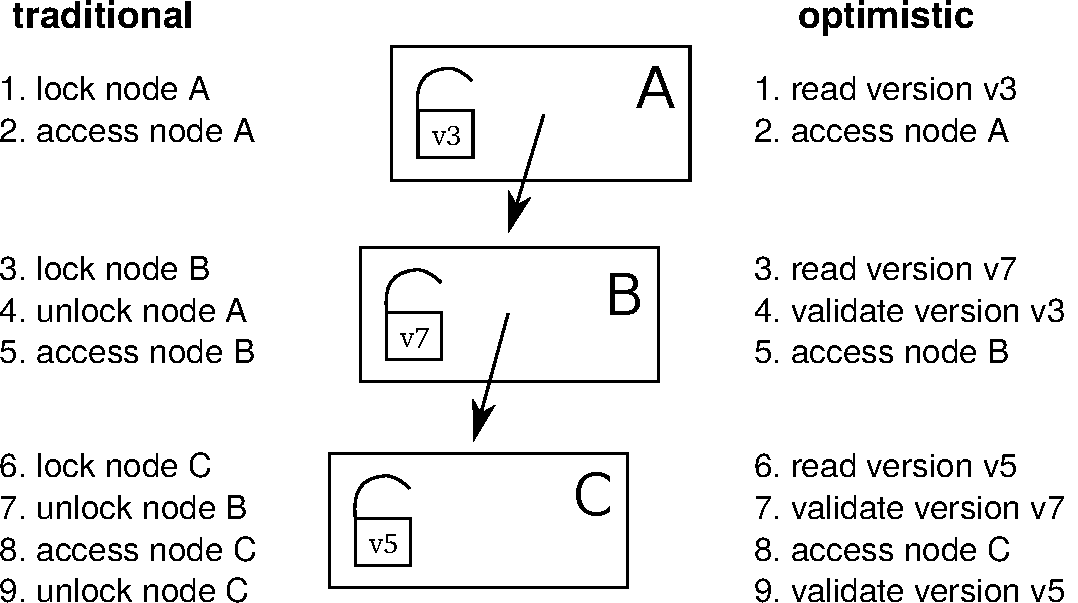
\includegraphics[width=0.65\linewidth]{olcall.pdf}
  \vspace{0.2cm}
  \caption{Comparison of a lookup operation in a 3-level tree using traditional lock coupling (left-hand side) vs.~optimistic lock coupling (right-hand side).}
  \label{fig:olc}
\end{figure}

The traditional and most common lock-based synchronization protocol for B-trees is lock coupling, which interleaves lock acquisitions while holding at most two locks at a time.
If, as we observed earlier, optimistic locks have similar semantics as traditional locks, it is natural to ask whether lock coupling can be combined with optimistic locks.
And indeed the answer is yes: One can almost mechanically translate traditional lock coupling code to optimistic lock coupling code.
This is illustrated in Figure~\ref{fig:olc}, which compares the traversal in a tree of height 3 using traditional and optimistic locks.
As the figure shows, the main difference is that locking is translated to reading the version and that unlocking becomes validation of the previously read version.
This simple change provides efficient lock-free tree traversal without the need to design a complex synchronization protocol.

It is important to emphasize the conceptual simplicity of OLC in comparison to data structures that use custom protocols like the Bw-tree~\cite{DBLP:conf/icde/LevandoskiLS13a}.
To implement lock-free access, the Bw-tree requires an indirection table, delta nodes, complex splitting and merging logic, retry logic, etc.
OLC, on the other hand, can directly be applied to B-trees mostly by adding the appropriate optimistic locking code and without modifying the node layout itself.
Therefore, OpenBw-Tree, an open source implementation of the Bw-tree, requires an order of magnitude more code than a B-tree based on OLC\footnote{Both implementations are available on GitHub: \url{https://github.com/wangziqi2016/index-microbench}}.
Given how difficult it is to develop, validate, and debug lock-free code, simplicity is obviously a major advantage.

\subsection{Correctness Aspects}

\begin{figure}
  % \centering
  %[basicstyle=\normalsize\ttfamily,showstringspaces=false,columns=fullflexible,breaklines=false,breakatwhitespace=true,numbers=none,numberstyle=\small,style=C,keepspaces=true]
\begin{lstlisting}[basicstyle=\ttfamily,language=C++,numbers=left,numberstyle=\small]
std::atomic<BTreeNode*> root;

// search for key in B+tree, returns payload in resultOut
bool lookup(Key key, Value& resultOut) {
   BTreeNode* node = root.load();
   uint64_t nodeVersion = node->readLockOrRestart();
   if (node != root.load()) // make sure the root is still the root
      restart();

   BTreeInner<Key>* parent = nullptr;
   uint64_t parentVersion = 0;

   while (node->isInner()) {
      auto inner = (BTreeInner*)node;

      // unlock parent and make current node the parent
      if (parent)
         parent->readUnlockOrRestart(parentVersion);
      parent = inner;
      parentVersion = nodeVersion;

      // search for next node
      node = inner->findChild(key);
      // validate 'inner' to ensure that 'node' pointer is valid
      inner->checkOrRestart(nodeVersion);
      // now it safe to dereference 'node' pointer (read its version)
      nodeVersion = node->readLockOrRestart();
   }

   // search in leaf and retrieve payload
   auto leaf = (BTreeLeaf*)node;
   bool success = leaf->findValue(key, resultOut);

   // unlock everything
   if (parent)
      parent->readUnlockOrRestart(parentVersion);
   node->readUnlockOrRestart(nodeVersion);

   return success;
}
\end{lstlisting}
  \vspace{0.2cm}
  \caption{B-tree lookup code using OLC. For simplicity, the restart logic is not shown.}
  \label{fig:lookup}
\end{figure}

So far, we have introduced the high-level ideas behind OLC and have stressed its similarity to traditional lock coupling.
Let us now discuss some cases where the close similarity between lock coupling and OLC breaks down.
To make this more concrete, we show the B-tree lookup code in Figure~\ref{fig:lookup}.
In the code, \texttt{readLockOrRestart} reads the lock version and \texttt{readUnlockOrRestart} validates that the read was correct.

One issue with OLC is that any pointer speculatively read from a node may point to invalid memory (if that node is modified concurrently).
Dereferencing such a pointer (e.g., to read its optimistic lock), may cause a segmentation fault or undefined behavior.
In the code shown in Figure~\ref{fig:lookup}, this problem is prevented by the extra check in line 25, which ensures that the read from the node containing the pointer was correct.
Without this additional validation, the code would in line 27 dereference the pointer speculatively read in line 23.
Note that the implementation of \texttt{checkOrRestart} is actually identical to \texttt{readUnlockOrRestart}.
We chose to give it a different name to highlight the fact that this extra check would not be necessary with read/write locks.

Another potential issue with optimistic locks is code that does not terminate.
Code that speculatively accesses a node, like an intra-node binary search, should be written in a way such that it always terminates---even in the presence of concurrent writes.
Otherwise, the validation code that detects the concurrent write will never run.
The binary search of a B-tree, for example, needs to be written in such a way that each comparison makes progress.
For some data structures that do not require loops in the traversal code (like ART) termination is trivially true.

\subsection{Implementation Details}

% implementation, efficiency
To implement an optimistic lock, one can combine the lock and the version counter into a single 64-bit\footnote{Even after subtracting one bit for the lock status, a back-of-the-envelope calculation can show that 63 bits are large enough to never overflow in practice.} word~\cite{artsync}.
A typical read operation will therefore merely consist of reading this version counter atomically.
In C++11 this can be implemented using the \texttt{std::atomic} type.

On x86, atomic reads are cheap because of x86's strong memory order guarantees.
No memory fences are required for sequentially-consistent loads, which are translated (by both GCC and clang) into standard \texttt{MOV} instructions.
Hence, the only effect of \texttt{std::atomic} for loads is preventing instruction re-ordering.
This makes version access and validation cheap.
Acquiring and releasing an optimistic lock in exclusive mode has comparable cost to a traditional lock:
A fairly expensive sequentially-consistent store is needed for acquiring a lock, while a standard \texttt{MOV} suffices for releasing it.
A simple sinlock-based implementation of optimistic locks can be found in the appendix of an earlier paper~\cite{artsync}.

OLC code must be able to handle restarts since validation or lock upgrade can fail due to concurrent writers.
Restarts can easily be implemented by wrapping the data structure operation in a loop (for simplicity not shown in Figure~\ref{fig:lookup}).
Such a loop also enables limiting the number of optimistic retry operations and falling back to pessimistic locking in cases of very heavy contention.
The ability to fall back to traditional locking is a major advantage of OLC in terms of robustness over lock-free approaches, which do not have this option.

In addition to the optimistic shared mode and the exclusive mode, optimistic locks also support a ``shared pessimistic'' mode, which physically acquires the lock in shared mode (allowing multiple concurrent readers but no writers).
This mode is useful for table (or range) scans that touch many tuples on a leaf page (which would otherwise easily abort).
Finally, let us mention that large range scans and table scans, should be broken up into several per-node traversals as is done in the LeanStore~\cite{leanstore} system.

Like all lock-free data structures, but unlike traditional locking and Hardware Transactional Memory~\cite{DBLP:conf/hpca/KarnagelDRLLSL14,DBLP:journals/pvldb/MakreshanskiLS15,htmtkde}, OLC requires care when deleting (and reusing) nodes.
The reason is that a deleting thread can never be sure that a node can be reclaimed because other threads might still be optimistically reading from that node.
Therefore, standard solutions like epoch-based reclamation~\cite{DBLP:conf/sosp/TuZKLM13}, hazard pointers~\cite{DBLP:journals/tpds/Michael04}, or optimized hazard pointers~\cite{DBLP:conf/spaa/BalmauGHZ16} need to be used.
These memory reclamation techniques are, however, largely orthogonal to the synchronization protocol itself.

%-lock-free is not a strong guarantee

\newpage
\section{Evaluation}\label{sec:evaluation}

Let us now experimentally evaluate the overhead and scalability of OLC.
For the experiments, we use an in-memory B+tree implemented in C++11 using templates, which is configured to use nodes of 4096 bytes, random 8 byte keys, and 8 byte payloads.
Based on this B-tree, we compare the following synchronization approaches:
\begin{itemize}
\item an OLC implementation\footnote{An almost identical OLC implementation is available on github: \url{https://github.com/wangziqi2016/index-microbench/tree/master/BTreeOLC}}
\item a variant based on traditional lock coupling and read/write locks
\item the unsynchronized B-tree, which obviously is only correct for read-only workloads but allows measuring the overhead of synchronization
\end{itemize}
Note that earlier work has compared the OLC implementation with a Bw-tree implementation~\cite{buzzword} and other state-of-the-art in-memory index structures.

We use a Haswell EP system with an Intel Xeon E5-2687W v3 CPU, which has 10 cores (20 ``Hyper-Threads'') and 25~MB of L3 cache.
The system is running Ubuntu 18.10 and we use GCC 8.2.0 to compile our code.
The CPU counters are obtained using the Linux perf API\footnote{We use the following convenience wrapper: \url{https://github.com/viktorleis/perfevent}}.

\begin{table}
  \caption{Performance and CPU counters for lookup and insert operations in a B-tree with 100M keys. We perform 100M operations and normalize the CPU counters by that number.}
  \label{tab:overhead}
  \centering
  \begin{tabular}{lrrrrrrr}\toprule
                    &         &        &        & instruc-  & L1     & L3     & branch \\
                    & threads & M op/s & cycles & tions & misses & misses & misses \\\midrule
lookup (no sync.)   & 1       & 1.72   & 2028   & 283     & 39.1   & 14.9   & 16.1   \\
lookup (OLC)        & 1       & 1.65   & 2107   & 370     & 43.9   & 15.1   & 16.7   \\
lookup (lock coup.) & 1       & 1.72   & 2078   & 365     & 42.3   & 16.9   & 15.7   \\\midrule
insert (no sync.)   & 1       & 1.51   & 2286   & 530     & 59.8   & 31.1   & 17.3   \\
insert (OLC)        & 1       & 1.50   & 2303   & 629     & 61.2   & 31.1   & 16.5   \\
insert (lock coup.) & 1       & 1.41   & 2473   & 644     & 61.0   & 31.0   & 17.2   \\\midrule
lookup (no sync.)   & 10      & 15.48  & 2058   & 283     & 38.6   & 15.5   & 16.0   \\
lookup (OLC)        & 10      & 14.60  & 2187   & 370     & 43.8   & 15.8   & 16.8   \\
lookup (lock coup.) & 10      & 5.71   & 5591   & 379     & 54.2   & 17.0   & 14.8   \\\midrule
insert (no sync.)   & 10      & -      & -      & -       & -      & -      & -      \\
insert (OLC)        & 10      & 10.46  & 2940   & 656     & 62.0   & 32.5   & 16.8   \\
insert (lock coup.) & 10      & 7.55   & 4161   & 667     & 75.0   & 28.6   & 16.2   \\
    \bottomrule
\end{tabular}
\end{table}

Table~\ref{tab:overhead} compares the performance and CPU counters for lookup and insert operations in a B-tree with 100M keys.
With {\em single-threaded} execution, we observe that all three approaches have very similar performance.
Adding traditional or optimistic locks to unsynchronized B-tree code results in up to 30\% of additional instructions without affecting single-threaded performance much.

\begin{figure}
  \centering
  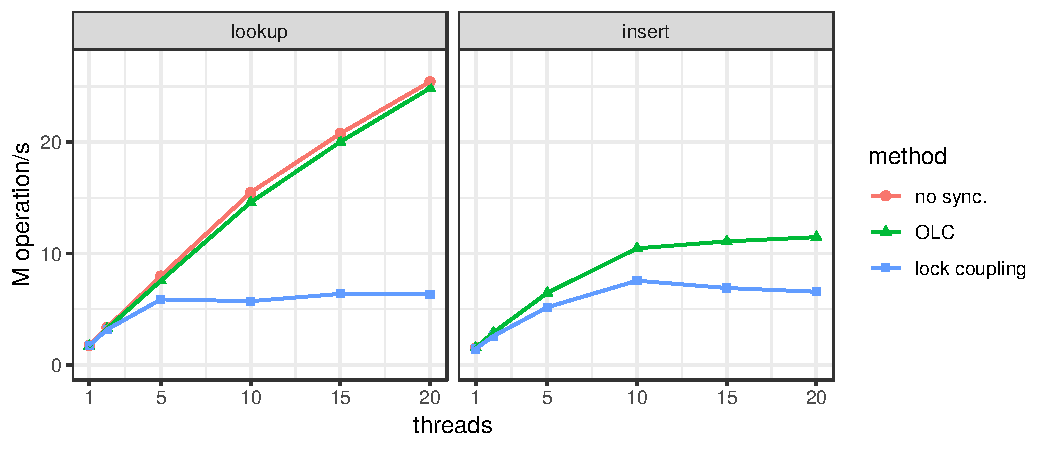
\includegraphics[width=\linewidth]{scale.pdf}
  \vspace{0.2cm}
  \caption{Scalability on 10-core system for B-tree operations (100M values).}
  \label{fig:scale}
\end{figure}

As Figure~\ref{fig:scale} shows, the results change dramatically once we use multiple threads.
For lookup, the scalability of OLC is near-linear up to 20 threads, even though the system has only 10 ``real cores''.
The OLC scalability for insert is also respectable (though not quite as linear because multi-threaded insertion approaches the memory bandwidth of our processor).
The figure also shows that the results of traditional lock coupling with read/write locks are significantly worse than OLC.
With 20 threads, lookup with OLC is 3.9$\times$ faster than traditional lock coupling.

\section{Summary}\label{sec:conc}

Optimistic Lock Coupling (OLC) is an effective synchronization method that combines the simplicity of traditional lock coupling with the superior scalability of lock-free approaches.
OLC is widely applicable and has already been successfully used to synchronize several data structures, including B-trees, binary search trees, and different trie variants.
These features make it highly attractive for modern database systems as well as performance-critical systems software in general.

\begin{thebibliography}{10}

\bibitem{DBLP:conf/spaa/BalmauGHZ16}
O.~Balmau, R.~Guerraoui, M.~Herlihy, and I.~Zablotchi.
\newblock Fast and robust memory reclamation for concurrent data structures.
\newblock In {\em SPAA}, 2016.

\bibitem{DBLP:journals/acta/BayerS77}
R.~Bayer and M.~Schkolnick.
\newblock Concurrency of operations on {B}-trees.
\newblock {\em Acta Informatica}, 9, 1977.

\bibitem{hot}
R.~Binna, E.~Zangerle, M.~Pichl, G.~Specht, and V.~Leis.
\newblock {HOT}: A height optimized trie index for main-memory database
  systems.
\newblock In {\em SIGMOD}, 2018.

\bibitem{DBLP:conf/ppopp/BronsonCCO10}
N.~G. Bronson, J.~Casper, H.~Chafi, and K.~Olukotun.
\newblock A practical concurrent binary search tree.
\newblock In {\em PPOPP}, 2010.

\bibitem{DBLP:conf/vldb/ChaHKK01}
S.~K. Cha, S.~Hwang, K.~Kim, and K.~Kwon.
\newblock Cache-conscious concurrency control of main-memory indexes on
  shared-memory multiprocessor systems.
\newblock In {\em VLDB}, 2001.

\bibitem{intel}
I.~Cutress.
\newblock {Intel} goes for 48-cores: {Cascade-AP} with multi-chip package
  coming soon.
\newblock
  \url{https://www.anandtech.com/show/13535/intel-goes-for-48cores-cascade-ap},
  2018 (accessed January, 2019).

\bibitem{DBLP:conf/cidr/FaleiroA17}
J.~M. Faleiro and D.~J. Abadi.
\newblock Latch-free synchronization in database systems: Silver bullet or
  fool's gold?
\newblock In {\em CIDR}, 2017.

\bibitem{DBLP:journals/ftdb/Graefe11}
G.~Graefe.
\newblock Modern {B}-tree techniques.
\newblock {\em Foundations and Trends in Databases}, 3(4), 2011.

\bibitem{DBLP:conf/hpca/KarnagelDRLLSL14}
T.~Karnagel, R.~Dementiev, R.~Rajwar, K.~Lai, T.~Legler, B.~Schlegel, and
  W.~Lehner.
\newblock Improving in-memory database index performance with
  {Intel}\({}^{\mbox{{\textregistered}}}\) transactional synchronization
  extensions.
\newblock In {\em HPCA}, 2014.

\bibitem{DBLP:journals/tods/LehmanY81}
P.~L. Lehman and S.~B. Yao.
\newblock Efficient locking for concurrent operations on {B}-trees.
\newblock {\em {ACM} Trans. Database Syst.}, 6(4), 1981.

\bibitem{leanstore}
V.~Leis, M.~Haubenschild, A.~Kemper, and T.~Neumann.
\newblock Leanstore: In-memory data management beyond main memory.
\newblock In {\em ICDE}, 2018.

\bibitem{art}
V.~Leis, A.~Kemper, and T.~Neumann.
\newblock The adaptive radix tree: {ARTful} indexing for main-memory databases.
\newblock In {\em ICDE}, 2013.

\bibitem{htmtkde}
V.~Leis, A.~Kemper, and T.~Neumann.
\newblock Scaling {HTM}-supported database transactions to many cores.
\newblock {\em {IEEE} Trans. Knowl. Data Eng.}, 28(2), 2016.

\bibitem{artsync}
V.~Leis, F.~Scheibner, A.~Kemper, and T.~Neumann.
\newblock The {ART} of practical synchronization.
\newblock In {\em DaMoN}, 2016.

\bibitem{DBLP:conf/icde/LevandoskiLS13a}
J.~J. Levandoski, D.~B. Lomet, and S.~Sengupta.
\newblock The {Bw}-tree: A {B}-tree for new hardware platforms.
\newblock In {\em ICDE}, 2013.

\bibitem{DBLP:journals/pvldb/MakreshanskiLS15}
D.~Makreshanski, J.~J. Levandoski, and R.~Stutsman.
\newblock To lock, swap, or elide: On the interplay of hardware transactional
  memory and lock-free indexing.
\newblock {\em {PVLDB}}, 8(11), 2015.

\bibitem{DBLP:dblp_conf/eurosys/MaoKM12}
Y.~Mao, E.~Kohler, and R.~T. Morris.
\newblock Cache craftiness for fast multicore key-value storage.
\newblock In {\em EuroSys}, 2012.

\bibitem{DBLP:journals/tpds/Michael04}
M.~M. Michael.
\newblock Hazard pointers: Safe memory reclamation for lock-free objects.
\newblock {\em {IEEE} Trans. Parallel Distrib. Syst.}, 15(6), 2004.

\bibitem{DBLP:journals/jacm/ShalevS06}
O.~Shalev and N.~Shavit.
\newblock Split-ordered lists: Lock-free extensible hash tables.
\newblock {\em J. {ACM}}, 53(3), 2006.

\bibitem{amd}
A.~Shilov.
\newblock {AMD} previews {EPYC} ‘{Rome}’ processor: Up to 64 {Zen} 2 cores.
\newblock
  \url{https://www.anandtech.com/show/13561/amd-previews-epyc-rome-processor-up-to-64-zen-2-cores},
  2018 (accessed January, 2019).

\bibitem{DBLP:conf/sosp/TuZKLM13}
S.~Tu, W.~Zheng, E.~Kohler, B.~Liskov, and S.~Madden.
\newblock Speedy transactions in multicore in-memory databases.
\newblock In {\em SOSP}, 2013.

\bibitem{buzzword}
Z.~Wang, A.~Pavlo, H.~Lim, V.~Leis, H.~Zhang, M.~Kaminsky, and D.~Andersen.
\newblock Building a {Bw}-tree takes more than just buzz words.
\newblock In {\em SIGMOD}, 2018.

\end{thebibliography}


%\bibliographystyle{abbrv}
%\bibliography{main}

\end{document}

\end{article}



\end{articlesection}

% put the news items below- there can be multiple news sections
% each with its own title
% news will usually have an author as well as a title,
% e.g. TCDE elections
% news articles are in the same format as letters
% typically, news articles will be stored in a directory called "news"

%\begin{newssection}{News headline}

% insert news items here; news will typically have authors
% see the Sept. 2018 issue for an example

%\begin{news}{news item title}
%{author name}{author affiliation}
%\input{news/news-article.tex}
%\end{news}
%
%\newpage


%\end{newssection}

\begin{callsection}

%  This section will be empty for your version
%
%  Calls for papers section.  Use the callsection environment.
%  Each call for papers is contained in an call environment, where the single
%  required options to \begin{call} is the name of the conference.
% typically calls are stored in a "calls" directory
%
%\begin{call}{name of conference}
%\centerline{\includegraphics[width=\textwidth, bb= 0 0 590 760]{calls/conference-name.pdf}}
%\end{call}
%\begin{call}{ICDE 2019 Conference}
%\centerline{\includegraphics[width=\textwidth, bb= 0 0 610 790] {../Dec-2018/calls/icde19.pdf}}
%\centerline{\includegraphics[width=\textwidth, bb= 0 0 590 760] {calls/icde19.pdf}}
%\end{call}
\begin{call}{TCDE Membership Form}
%\centerline{\includegraphics[width=\textwidth, bb= 0 0 610 790]
%\centerline{
\includegraphics[width=\textwidth, bb= 0 0 590 760] {../Dec-2018/calls/tcde.pdf}}
\centerline{
\includegraphics[width=\textwidth, bb= 0 0 590 760] {../2020-09/calls/tcde.pdf}}
\end{call}

\end{callsection}

\end{bulletin}
\end{document}
